\documentclass{article}
\pdfoutput=1

%%% Packages %%%

% Graphics
\usepackage{graphicx}
\usepackage[caption=false,font=footnotesize]{subfig}

% Formatting
\usepackage{color}
\usepackage{amsmath}
\usepackage{amsfonts}
\usepackage{bbm}

\usepackage[scaled]{helvet}
\renewcommand*\familydefault{\sfdefault} %% Only if the base font of the document is to be sans serif
\usepackage[T1]{fontenc}

% Environments
\usepackage{IEEEtrantools}
\usepackage{algorithm}
\usepackage{algorithmic}

% Logic
\usepackage{ifthen}
\usepackage{etoolbox}

% References
\usepackage{natbib}

% Drawing
\usepackage{tikz}
\usepackage{pgfplots}
 \usetikzlibrary{plotmarks}
 \pgfplotsset{compat=newest}
 \pgfplotsset{plot coordinates/math parser=false}
 \usepgfplotslibrary{external}
 \tikzexternalize[prefix=tikz/]

\graphicspath{{figures/}}

%%% Macros %%%
%%% Theorem environments %%%
\newtheorem{theorem}{Theorem}[section]
\newtheorem{lemma}[theorem]{Lemma}
\newtheorem{proposition}[theorem]{Proposition}
\newtheorem{corollary}[theorem]{Corollary}
\newtheorem{model}[theorem]{Model}

\newenvironment{proof}[1][Proof]{\begin{trivlist}
\item[\hskip \labelsep {\bfseries #1}]}{\end{trivlist}}
\newenvironment{definition}[1][Definition]{\begin{trivlist}
\item[\hskip \labelsep {\bfseries #1}]}{\end{trivlist}}
\newenvironment{example}[1][Example]{\begin{trivlist}
\item[\hskip \labelsep {\bfseries #1}]}{\end{trivlist}}
\newenvironment{remark}[1][Remark]{\begin{trivlist}
\item[\hskip \labelsep {\bfseries #1}]}{\end{trivlist}}

\newcommand{\qed}{\nobreak \ifvmode \relax \else
      \ifdim\lastskip<1.5em \hskip-\lastskip
      \hskip1.5em plus0em minus0.5em \fi \nobreak
      \vrule height0.75em width0.5em depth0.25em\fi}
%%%%%%%%%%%%%%%%%%%%%%%%%%%%%%


\newcommand{\real}{\mathbb{R}}

\newcommand{\lhood}{l}
\newcommand{\nconst}[1]{K_{#1}}

\newcommand{\lsspace}{\mathcal{X}}
\newcommand{\lsdim}{{d_{\ls{}}}}
\newcommand{\priorden}{p}
\newcommand{\postden}{\pi}
\newcommand{\seqden}[1]{\pi_{#1}}
\newcommand{\seqdenapprox}[1]{\hat{\pi}_{#1}}
\newcommand{\impden}{q}
\newcommand{\incimpden}[1]{q_{#1}}

\newcommand{\logprior}{M}
\newcommand{\loglhood}{L}
\newcommand{\logseqden}[1]{\Xi_{#1}}
\newcommand{\logseqdenapprox}[1]{\hat{\Xi}_{#1}}

\newcommand{\sn}[1]{z_{#1}}
\newcommand{\snchange}[1]{\xi_{#1}}

\newcommand{\lsmnapprox}[1]{\hat{m}_{#1}}
\newcommand{\lsvrapprox}[1]{\hat{P}_{#1}}


% Particle flow
\newcommand{\flowbm}[1]{\epsilon_{#1}}          % Particle flow Brownian motion
\newcommand{\flowdrift}[1]{\zeta_{#1}}          % Particle flow drift
\newcommand{\flowdiffuse}[1]{\eta_{#1}}         % Particle flow diffusion
\newcommand{\flowcov}[1]{D_{#1}}                % Particle flow "Covariance" matrix
\newcommand{\dsf}{\gamma}                % Particle flow diffusion scale factor

\newcommand{\lgmomapprox}[1]{\hat{\lgmom}_{#1}}       % Linear observation matrix formed by differentiation of the observation function
\newcommand{\obapprox}[1]{\hat{y}_{#1}}

\newcommand{\flowdriftapprox}[1]{\hat{\zeta}_{#1}}      % Approximate (actual) particle flow drift
\newcommand{\flowdiffuseapprox}[1]{\hat{\eta}_{#1}}     % Approximate (actual) particle flow diffu






%%% Basic maths stuff %%%
\newcommand{\zmatrix}{\mathsf{0}}
\newcommand{\idmatrix}{\mathsf{I}}
\newcommand{\half}{\frac{1}{2}}

%%% Functions and operators %%%
\newcommand{\minv}{^{-1}}
\newcommand{\determ}[1]{\left|#1\right|}
\newcommand{\magn}[1]{\left|#1\right|}
\newcommand{\pd}[3]{\left.\frac{\partial #1}{\partial #2}\right|_{#3}}
\newcommand{\npd}[4]{\left.\frac{\partial^{#1} #2}{\partial #3}\right|_{#4}}
\newcommand{\expect}[1]{\mathbb{E}_{#1}}
\newcommand{\variance}[1]{\mathbb{V}_{#1}}
\newcommand{\bigo}[1]{\mathcal{O}\left(#1\right)}
\newcommand{\prob}{P}
\newcommand{\indic}[1]{\mathbbm{1}_{#1}}
\DeclareMathOperator{\sinc}{sinc}
\DeclareMathOperator{\trace}{Tr}
\newcommand{\degr}{^{\circ}}
\newcommand{\rightasconverge}{\stackrel{a.s.}{\rightarrow}}
\newcommand{\leftasconverge}{\stackrel{a.s.}{\leftarrow}}

%%% Probability spaces %%%
\newcommand{\reals}{\mathbb{R}}

%%% Time, indexes, etc. %%%
\newcommand{\ti}{n}
\newcommand{\dct}[1]{t_{#1}}
\newcommand{\timax}{N}

%%% States, observations, etc. %%%
\newcommand{\ls}[1]{x_{#1}}
\newcommand{\ob}[1]{y_{#1}}
\newcommand{\rls}[1]{u_{#1}}
\newcommand{\mls}[1]{z_{#1}}

%%% Distributions %%%
\newcommand{\normalden}[3]{\mathcal{N}\left(#1\left|\vphantom{#1}#2,#3\right.\right)}
\newcommand{\uniformden}[2]{\mathcal{U}\left(\left[#1,#2\right]\right)}
\newcommand{\dirac}[1]{\delta_{#1}}
\newcommand{\gammaden}[3]{\mathcal{G}\left(#1\left|#2,#3\right.\right)}
\newcommand{\studenttden}[4]{\mathcal{ST}\left(#1|#2,#3,#4\right)}


%%% Particle things %%%
\newcommand{\pss}[1]{^{(#1)}}

%%% Densities %%%
\newcommand{\den}{p}
\newcommand{\pden}{\hat{p}}
%\newcommand{\priorden}{\varpi}
\newcommand{\transden}{f}
\newcommand{\obsden}{g}
%\newcommand{\loglhood}{\mathcal{L}}

%%% Particle filter things %%%
%\newcommand{\impden}[1]{q_{#1}}
\newcommand{\partden}[1]{\eta_{#1}}
\newcommand{\pw}[1]{w_{#1}}
\newcommand{\npw}[1]{\bar{w}_{#1}}
\newcommand{\predpw}[1]{\hat{w}_{#1}}
\newcommand{\naw}[1]{\bar{v}_{#1}}
\newcommand{\respw}[1]{\tilde{w}_{#1}}
\newcommand{\anc}[2]{a_{#1}^{(#2)}}
\newcommand{\replic}[2]{R_{#1}^{(#2)}}
\newcommand{\ess}[1]{\mathbf{N}_{\text{EFF},#1}}
\newcommand{\lsrm}[1]{\tilde{x}_{#1}}

%%% MCMC things %%%
\newcommand{\mhkernel}{K}
\newcommand{\mhaccept}{\alpha}
\newcommand{\nummhsteps}{M}

%%% Monte Carlo things %%%
\newcommand{\numpart}{\mathbf{N}}
\newcommand{\testfunc}{\zeta}
\newcommand{\unnormden}{\gamma}

%%% State space models %%%
\newcommand{\transfun}{\phi}
\newcommand{\obsfun}{\psi}
\newcommand{\transinnov}[1]{u_{#1}}
\newcommand{\obsinnov}[1]{v_{#1}}

%%% Linear Gaussian model %%%
\newcommand{\lgmtm}{F}
\newcommand{\lgmtnm}{G}
\newcommand{\lgmtv}{Q}
\newcommand{\lgmom}{H}
\newcommand{\lgmov}{R}


%%% MACROS FOR MATHEMATICAL NOTATION IN COMPOSITE PROPOSAL PAPER %%%

% Functions and operators
\newcommand{\magdet}[1]{\left| #1 \right|}         % Magnitude of the determinant
\newcommand{\normal}[3]{\mathcal{N}\left(#1\left|#2,#3\right.\right)}       % Normal density
\newcommand{\studentt}[4]{\mathcal{ST}\left(#1|#2,#3,#4\right)} % Student-t density
% \newcommand{\npd}[4]{\left.\frac{\partial^{#1} #2}{\partial #3^{#1}}\right|_{#4}}
\newcommand{\pdv}[2]{\frac{\partial #1}{\partial #2}}
\newcommand{\ppdv}[2]{\frac{\partial^2 #1}{\partial #2^2}}
\newcommand{\mpdv}[3]{\frac{\partial^2 #1}{\partial #2 \partial #3}}
\newcommand{\npdv}[3]{\frac{\partial^{#1} #2}{\partial #3^{#1}}}
\newcommand{\nmpdv}[5]{\frac{\partial^{#1} #3}{\partial^{#2} #4 \partial #5}}

% Basics
% \newcommand{\rt}{t}                             % Real time
\newcommand{\pt}{\lambda}                       % Pseudo-time
\newcommand{\dpt}{\delta\lambda}                % A little bit of pseudo-time
% \newcommand{\ls}[1]{x_{#1}}                     % Latent state
\newcommand{\dls}{\delta x}                     % A little bit of latent state
% \newcommand{\ob}[1]{y_{#1}}                     % Observation
\newcommand{\mix}[1]{\xi_{#1}}                  % Mixing auxiliary variable
\newcommand{\els}[1]{u_{#1}}                    % Extra latent state

% % Particle shizzle
% \newcommand{\pss}[2][]{^{(#2)#1}}               % Particle superscript
% \newcommand{\pw}[1]{w_{#1}}                     % Particle weight
% \newcommand{\predpw}[1]{\hat{w}_{#1}}           % Predictive particle weight
% \newcommand{\npw}[1]{\bar{w}_{#1}}              % Normalised particle weight
% \newcommand{\naw}[1]{\bar{v}_{#1}}              % Normalised auxiliary weight
% \newcommand{\anc}[1]{a_{#1}}                    % Particle ancestor

% Densities
% \newcommand{\transden}{f}                       % Transition density
% \newcommand{\obsden}{g}                         % Observation density
% \newcommand{\impden}{q}                         % Importance density
% \newcommand{\partden}{\eta}                     % Unweighted particle distribution
% \newcommand{\artden}{\rho}                      % Artificial conditional density
\newcommand{\oiden}[1]{\pi_{#1}}                % Optimal importance density
% % \newcommand{\logoiden}[1]{\Xi_{#1}}             % Log of the optimal importance density
% \newcommand{\logoidenapprox}[1]{\hat{\Xi}_{#1}} % Approximation of the log of the optimal importance density
\newcommand{\approxoiden}[2]{\hat{\pi}_{#1|#2}} % Approximation of the optimal importance density
\newcommand{\ctapproxoiden}[1]{\hat{\pi}_{#1}}
\newcommand{\augfiltden}[1]{\tilde{\pi}_{#1}}   % Augmented filtering density
\newcommand{\oinorm}[1]{K_{#1}}                 % Normalising constant for the optimal importance density
\newcommand{\augfiltnorm}[1]{\tilde{K}_{#1}}    % Normalising constant for the augmented filtering density

% Numbers
% \newcommand{\numpart}{N_F}                      % Number of filter particles
% \newcommand{\ess}[1]{N_{E,#1}}                  % Effective sample size

% Models
% \newcommand{\transfun}{\phi}                    % Transition function
% \newcommand{\obsfun}{h}                         % Observation function
% \newcommand{\transcov}{Q}                       % Transition covariance
% \newcommand{\obscov}{R}                         % Observation covariance
% \newcommand{\transmat}{F}                       % Linear transition matrix
% \newcommand{\obsmat}{H}                         % Linear observation matrix
% \newcommand{\transmean}{m}                      % Mean of the transition density (i.e. f(x_{t-1}))
\newcommand{\dof}{\nu}                          % Degrees of freedom of something student-t-ish

% Linear Gaussian things
% \newcommand{\lgoimean}[1]{\mu_{#1}}             % Linear Gaussian optimal importance density mean
% \newcommand{\lgoicov}[1]{\Sigma_{#1}}           % Linear Gaussian optimal importance density covariance
% \newcommand{\stdnorm}[1]{z_{#1}}                % Standard normal R.V.
% \newcommand{\obmn}[1]{\nu_{#1}}
% \newcommand{\obvr}[1]{S_{#1}}
% \newcommand{\obcvr}[1]{C_{#1}}
\newcommand{\obmnapprox}[1]{\hat{\mu}_{#1}}
\newcommand{\obvrapprox}[1]{\hat{\Sigma}_{#1}}
\newcommand{\obcvrapprox}[1]{\hat{C}_{#1}}

% Gaussian Transformation
\newcommand{\lgdecayfunc}{a}                    % Linear Gaussian decay function for OID transformation
\newcommand{\lgexpsf}{\gamma}                   % Linear Gaussian exponential scale factor for OID transformation
\newcommand{\lgupdmeanmat}[1]{\Gamma_{#1}}      % Mean mapping matrix for the OID transformation
\newcommand{\lgupdcov}[1]{\Omega_{#1}}          % Covariance matrix for the OID transformation
\newcommand{\lginfbm}[1]{\epsilon_{#1}}         % Brownian motion for the infinitesimal form of the OID transformation

% Linear Gaussian approximations
%\newcommand{\lgoimeanapprox}[2]{\hat{\mu}_{#1}(#2)}     % Mean of the Gaussian approximation to the OID at time #1 and state #2
%\newcommand{\lgoicovapprox}[2]{\hat{\Sigma}_{#1}(#2)}   % Covariance of the Gaussian approximation to the OID at time #1 and state #2
\newcommand{\lgoimnapprox}[2]{\hat{m}_{#1|#2}}      % Mean of the Gaussian approximation to the OID at time #1 and state #2
\newcommand{\lgoivrapprox}[2]{\hat{P}_{#1|#2}}    % Covariance of the Gaussian approximation to the OID at time #1 and state #2
\newcommand{\ctlgoimnapprox}[1]{\hat{m}_{#1}}
\newcommand{\ctlgoivrapprox}[1]{\hat{P}_{#1}}
%\newcommand{\lgoimeanapprox}[2][]{\ifstrempty{#1}{\hat{\mu}_{#2}}{\hat{\mu}_{#1|#2}}}
%\newcommand{\lgoicovapprox}[2][]{\ifstrempty{#1}{\hat{\Sigma}_{#2}}{\hat{\Sigma}_{#1|#2}}}

\newcommand{\transmeanapprox}[1]{\hat{\transfun}_{#1}} % Approximate transition mean
\newcommand{\lgmtvapprox}[1]{\hat{\lgmtv}_{#1}}   % Approximate transition covariance
\newcommand{\lgmovapprox}[1]{\hat{\lgmov}_{#1}}       % Approximate observation covariance
\newcommand{\lsfixed}{\ls{}^*}                          % Latent state around which we linearise
\newcommand{\logtrans}{M}                               % Log of the transition density
\newcommand{\logobs}{L}                                 % Log of the observation density

% State evolution SDE
\newcommand{\oudrift}[1]{A_{#1}}                % General O-U process drift term
\newcommand{\oudiffuse}[1]{B_{#1}}              % General O-U process diffusion term
\newcommand{\lserror}[2]{e_{#1|#2}}             % State error due to finite sampling



\newcommand{\flowtd}{\alpha}                    % Flow dervation transition density
\newcommand{\flowod}{\mathcal{L}}               % Flow derivation observation density
%\newcommand{\flowdriftapprox}[2]{\hat{\zeta}_{#1|#2}}      % Approximate (actual) particle flow drift
%\newcommand{\flowdiffuseapprox}[2]{\hat{\eta}_{#1|#2}}     % Approximate (actual) particle flow diffusion

% Simulation models - tracking
\newcommand{\pos}[1]{p_{#1}}           % Position
\newcommand{\vel}[1]{v_{#1}}           % Velocity
\newcommand{\bng}[1]{b_{#1}}               % Bearing
\newcommand{\ele}[1]{\eta_{#1}}                 % Elevation
\newcommand{\rng}[1]{r_{#1}}                    % Range
\newcommand{\hei}[1]{h_{#1}}                    % Height
\newcommand{\rngrt}[1]{s_{#1}}                  % Range rate
\newcommand{\terrain}{T}                        % Terrain height

% Simulation models - heartbeats
\newcommand{\amp}[1]{A_{#1}}                    % Amplitude
\newcommand{\wid}[1]{W_{#1}}                    % Width
\newcommand{\del}[1]{\tau_{#1}}                 % Delay
\newcommand{\freq}[1]{\omega_{#1}}              % Width
\newcommand{\pha}[1]{\psi_{#1}}                 % Phase
\newcommand{\bias}[1]{B_{#1}}                   % Bias





%%% Importance Densities %%%
\newcommand{\lgoimn}[1]{m_{#1}}
\newcommand{\lgoivr}[1]{P_{#1}}
\newcommand{\logoiden}[1]{\Xi_{#1}}
\newcommand{\logoidenapprox}[1]{\hat{\Xi}_{#1}}



\newcommand{\stdnorm}[1]{z_{#1}}
\newcommand{\artden}[1]{\rho_{#1}}
\newcommand{\fixed}{^*}


%%% Gaussian filter parameters %%%
\newcommand{\lsmn}[1]{m_{#1}}
\newcommand{\lsvr}[1]{P_{#1}}
\newcommand{\lspredmn}[1]{\hat{m}_{#1}}
\newcommand{\lspredvr}[1]{\hat{P}_{#1}}
\newcommand{\obmn}[1]{\mu_{#1}}
\newcommand{\obvr}[1]{\Sigma_{#1}}
\newcommand{\obcvr}[1]{C_{#1}}




%%% Environments %%%
\newenvironment{meta}[0]{\color{red} \em}{}



%%% Titles and stuff %%%
%\address{Cambridge University Engineering Department,Cambridge,UK.}
%\email{pb404@cam.ac.uk}
\title{Approximations of the Optimal Importance Density using Gaussian Particle Flow Importance Sampling}
\author{Pete Bunch and Simon Godsill}
\date{}



%%% DOCUMENT %%%

\begin{document}

\maketitle

\begin{abstract}
The crucial step in designing a particle filter for a particular application is the choice of importance density. The optimal scheme is to use the conditional posterior density of the state, but this cannot be sampled or calculated analytically in most case. In practice, approximations of this density are used, particularly Gaussian densities based on linearisation or the unscented transform. For many highly nonlinear or non-Gaussian models, these approximations can be poor, leading to degeneracy of the particle approximation or even complete divergence of the filter. In this paper, we study particle flow methods for sampling from probability densities, and in particular the analytically tractable ``Gaussian flow''. Particle flow methods work by first sampling from the prior and then moving particles continuously such that the evolution of their density corresponds to the progressive introduction of the likelihood. With nonlinear and non-Gaussian models, by performing a series of small state updates, each using a local Gaussian approximation, samples distributed approximately according to the posterior may be generated. The discrepancy between this approximation and the true density may be accommodated using a importance sampling. This Gaussian flow scheme is used to sample from the optimal importance density in a particle filter and shown to yield improvements in error and effective sample size.
\end{abstract}



%\keywords{particle filter, sequential Monte Carlo, optimal importance distribution}



\section{Introduction}

The particle filter is an algorithm used for sequential inference of a filtering distribution associated with a state-space model. A set of samples is advanced through time, drawn approximately from the filtering distribution. This is achieved by sampling at each time step from an importance distribution and then weighting the particles to account for the discrepancy between filtering and importance distributions. For a comprehensive introduction, see for example \citep{Cappe2007,Doucet2009}.

The principal challenge when designing a particle filter is the selection of the importance density. The simplest choice is often to sample from the transition model, resulting in the ``bootstrap filter'' of \citep{Gordon1993}. In many cases, such bootstrap proposals result in poor filter performance due to a mismatch in the areas of high probability between the prior and posterior densities.

Amongst others, \citet{Doucet2000a} demonstrated that the ideal choice of importance density for each particle is the conditional posterior given both the previous state and the new observation, dubbed the ``optimal importance density'' (OID). In all but a few cases, this cannot be calculated analytically. A popular solution is to use linearisation or the unscented transform to select a Gaussian importance density which approximates the OID for each particle \citep{Doucet2000a,Merwe2000}. However, such schemes can fail when the model is highly nonlinear or non-Gaussian, as the approximation is poor.

The effect of using a bad importance density (i.e. one which is not ``close'' to the OID) is that the variance of the importance weights is high, resulting in a degeneracy of the filter. In the worst cases, there may be no particles at all proposed in regions of high posterior probability, causing the filter to fail entirely. This problem is especially pronounced when the dimensionality of the state space is high --- there is simply more space for the particles to cover.

A common enhancement to the basic particle filter, which helps to alleviate the problems of degeneracy, is to include Markov chain Monte Carlo (MCMC) steps in order to rejuvenate a degenerate set of particles, a method named ``resample-move'' by \citet{Gilks2001}. When the importance sampling step has resulted in only a few useful particles in high probability areas, MCMC steps allow copies of these to be perturbed, so that they become better spread over the state space while still maintaining the correct distribution. While resample-move can often provide a useful fix for a struggling particle filter, it would be preferable to improve the initial importance sampling step so that such a fix is not required. There is, after all, a limit to what resample-move can practically achieve; if the importance sampling fails to put any particles in the right areas then a very large number of MCMC steps may be needed to get them there. In addition, an MCMC stage introduces new algorithm parameters which need to be tuned for effective operation, e.g. the number of MCMC steps per particle, and the proposal distribution.

Another way in which degeneracy may be mitigated is by introducing the effect of each observation gradually, so that particles may be progressively drawn towards peaks in the likelihood. This can be achieved by using a discrete set of bridging distributions which transition smoothly between the prior and posterior. Each one is targeted in turn using importance sampling and particle diversity is maintained using Metropolis-Hastings moves. Such ``annealing'' schemes have been suggested by, amongst others, \citet{Neal2001} (using MCMC) and \citet{DelMoral2006} (using Sequential Monte Carlo (SMC) samplers) for static inference problems, and by \citet{Godsill2001b,Gall2007,Deutscher2000,Oudjane2000} for particle filters.

It is possible to take the idea of bridging distributions to a limit and define a continuous sequence of distributions between the prior and the posterior. This device was used by \citet{Gelman1998} for the related task of simulating normalising constants, and has been used to design sophisticated assumed density filters \citep{Hanebeck2003a,Hanebeck2012,Hagmar2011}. More recently, particle filters have appeared which exploit the same principle, including the \emph{particle flow} methods described in series of papers including \citep{Daum2008,Daum2011d}, and the \emph{optimal transport} methods of \cite{Reich2011,Reich2012a}. A particle is first sampled from the prior (i.e. the transition) density, and then moved continuously according to some differential equation over an interval of \emph{pseudo-time}, such that the evolution in the density corresponds to the progressive introduction of the likelihood.

Although theoretically elegant and powerful, practical implementation of optimal transport or particle flow methods require a host of approximations to be made. First, even if the prior density were known, it would be often necessary to make approximations in order to find an appropriate flow. Second, when applying particle flow to the a filtering density, the prior is generally not known analytically, and must itself be approximated. Third, once an appropriate flow has been identified, it must usually then be integrated numerically.

In this paper we choose to move the particles according to a Gaussian flow, which is optimal for a linear Gaussian model, and which requires no numerical integration. Furthermore, it is possible to calculate pointwise the density associated with each particle trajectory. Rather than using this density directly as an approximation to the posterior, it is treated as the importance density to an importance sampler. Thus, we are able to correct for the discrepancies introduced by approximating the flow. Finally, we apply this particle flow proposal method to the OID of a particle filter, rather than to the filtering density itself. This allows the particle flow to be applied within the standard framework for particle filtering, and also avoids the need to use approximations of the predictive density.

We demonstrate the efficacy of Gaussian flow importance sampling for particle filtering with simulations on a number of challenging nonlinear models. Significant performance improvements are observed in error and effective sample size statistics. The new method delivers the greatest advantage when the prior and likelihood models have a Gaussian form, but the observation function is highly nonlinear.



\section{Importance Sampling and Particle Flows}

Consider the problem of sampling from a Bayesian posterior distribution over a hidden state variable $\ls{} \in \lsspace = \real^\lsdim$,
%
\begin{IEEEeqnarray}{rCl}
 \postden(\ls{}) & = & \frac{ \priorden(\ls{}) \lhood(\ls{}) }{ \nconst{} } \\
 \nconst{} & = & \int \priorden(\ls{}) \lhood(\ls{}) d\ls{}      .
\end{IEEEeqnarray}
%
in which $\priorden$ and $\postden$ are the prior and posterior densities respectively, which are assumed to exist, $\lhood$ is the likelihood and $\nconst{}$ is a normalising constant. We assume that this constant cannot be evaluated, and hence the posterior density is only available up to a constant of proportionality. Importance sampling may be used to draw from such posterior distributions \citep{Geweke1989,Liu2001a}. A set of $\numpart$ i.i.d. samples (or \emph{particles}, the two terms are used interchangeably throughout) is generated according to some importance distribution with density $\impden(\ls{})$ and each is assigned a weight,
%
\begin{IEEEeqnarray}{rCl}
 \pw{}\pss{i}  & = & \frac{ \priorden(\ls{}\pss{i}) \lhood(\ls{}\pss{i}) }{ \impden(\ls{}\pss{i}) } \nonumber \\
 \npw{}\pss{i} & = & \frac{ \pw{}\pss{i} }{ \sum_j \pw{}\pss{j} }     .
\end{IEEEeqnarray}
%
An estimator of a posterior expectation may then be written as a finite sum over this set of weighted samples, and it may be shown that this estimate converges almost surely to its true value as the number of particles becomes large \citep{Liu2001a},
%
\begin{IEEEeqnarray}{rCl}
 \sum_{i=1}^{\numpart} \npw{\ti}\pss{i} \phi(\ls{}\pss{i}) & \rightasconverge & \int \postden(\ls{}) \phi(\ls{}) d\ls{}     \nonumber       .
\end{IEEEeqnarray}

The effectiveness of such an importance sampler depends crucially on the choice of importance density. In general, the closer $\impden(\ls{})$ is to $\postden(\ls{})$, the better the estimates will be. Selecting a good importance density is therefore a foremost priority, but often proves challenging. One common approach is to use the prior as the importance density, meaning that,
%
\begin{IEEEeqnarray}{rCl}
 \impden(\ls{}) & = & \priorden(\ls{}) \nonumber \\
 \pw{}\pss{i}   & = & \lhood(\ls{}\pss{i})    .
\end{IEEEeqnarray}
%
This scheme has the advantage of simplicity and generality. The only requirement is that it should be possible to sample from the prior. However, it is inefficient, especially when the variance of the prior is much greater than that of the posterior, i.e. the likelihood is highly informative about the state. In this situation, the samples are widely spread over the state space, and only a few fall in the region of high likelihood. The consequence is that many have very low weight and posterior estimates are based on only a few significant particles; the resulting estimators are poor, having a high Monte Carlo variance. This is a fundamental difficulty for importance samplers. Good posterior sampling relies on having a good approximation of the posterior to begin with!

Particle flow and optimal transport methods are an alternative mechanism for generating posterior samples. They have been applied to Bayesian filtering and data assimilation problems by \cite{Daum2008,Daum2011d,Daum2013,Reich2011,Reich2012a}. The general principle is to begin with samples from the prior, then to move these according to some dynamics over an interval of pseudo-time such that the final values are distributed according to the posterior. One suitable way to achieve this is to define the following geometric density sequence over the interval $\pt \in \left[0,1\right]$,
%
\begin{IEEEeqnarray}{rCl}
 \seqden{\pt}(\ls{\pt}) & = & \frac{ \priorden(\ls{\pt}) \lhood(\ls{\pt})^{\pt} }{ \nconst{\pt} } \label{eq:density_sequence} \\
 \nconst{\pt}           & = & \int \priorden(\ls{}) \lhood(\ls{})^{\pt} d\ls{}      .
\end{IEEEeqnarray}
%
Since $\seqden{0} = \priorden$, initial particles may be sampled from the prior. These are then moved according to an ordinary (ODE) or stochastic (SDE) differential equation such that at every instant in pseudo-time each one is distributed according to the appropriate density in this sequence,
%
\begin{IEEEeqnarray}{rCl}
 \ls{\pt}\pss{i} & \sim & \seqden{\pt}(\ls{\pt})      .
\end{IEEEeqnarray}
%
At the end, since $\seqden{1} = \postden$, the final particles are distributed according to the posterior. Using the basic properties of Monte Carlo sampling, posterior expectations may now be approximated as a finite sum using this unweighted set of samples, and it may be shown again that this estimate converges almost surely to its true value as the number of particles becomes large,
%
\begin{IEEEeqnarray}{rCl}
 \frac{1}{\numpart} \sum_{i=1}^{\numpart} \phi(\ls{1}\pss{i}) & \rightasconverge & \int \postden(\ls{}) \phi(\ls{}) d\ls{}     \nonumber       .
\end{IEEEeqnarray}

The challenge in applying such a particle flow sampler comes in finding suitable dynamics with which to move the particles such that the correct density is maintained throughout. In general, this cannot be achieved analytically, and approximations are called for (see aforesaid references). While these may be effective, they result in the loss of asymptotic consistency, and the introduction of bias which is not easily quantified.

The approach adopted in this paper, suggested by \cite{Reich2012}, is to combine particle flow with importance sampling, by using a particle flow approximation of the posterior as an importance density; thus we retain asymptotic consistency of posterior estimators. The pseudo-time interval is divided up into many small increments, and for each one the particles are moved according to a \emph{Gaussian flow} approximation of the exact flow (i.e. that corresponding to \eqref{eq:density_sequence} precisely). This Gaussian flow defines an analytically tractable dynamical system which allows the density associated with the resulting particle trajectories to be evaluated pointwise. The state values generated in this manner are treated as proposals within an importance sampler, and each is assigned an appropriate weight.



\section{Sampling with Gaussian Flows}

\subsection{Gaussian Flows for Linear Gaussian Models}

A difficulty in employing particle flow methods, encountered by both \cite{Daum2011d,Reich2011}, is the need for numerical integration. Particle dynamics corresponding to the density sequence \eqref{eq:density_sequence} are derived in the form of an ODE or SDE, which must then be solved numerically in order to find the new particle locations. Simple solvers may be unstable and more complex solvers very expensive to use. In addition, this numerical integration will introduce errors into the sampling procedure and hence alter the final particle distribution. We can avoid numerical integration by using approximations based on a Gaussian flow.

When the model used is linear and Gaussian, the exact flow for particle motion may be derived analytically. Suppose the likelihood takes the form of an observation $\ob{}\in\obspace = \real^{\obdim}$ which is linearly dependent on the state with Gaussian noise, and that the prior is also Gaussian.
%
\begin{model} \label{mod:linear_gaussian}
\begin{IEEEeqnarray}{rCl}
 \priorden(\ls{}) & = & \normalden{\ls{}}{\lsmn{0}}{\lsvr{0}} \\
 \lhood(\ls{})    & = & \normalden{\ob{}}{\lgmom\ls{}}{\lgmov}
\end{IEEEeqnarray}
$\lsvr{0}$ and $\lgmov$ are positive definite covariance matrices.
\end{model}
%
For this model, the following properties may be established.
%
\begin{proposition} \label{prop:linear_gaussian_density_sequence}
The density sequence may be calculated analytically,
%
\begin{IEEEeqnarray}{rCl}
 \seqden{\pt} & = & \normalden{\ls{\pt}}{\lsmn{\pt}}{\lsvr{\pt}} \label{eq:linear_gaussian_density_sequence} \\
 \lsvr{\pt} & = & \left(\lsvr{0}^{-1} + \pt \lgmom^T \lgmov^{-1} \lgmom\right)^{-1} \nonumber \\
 & = & \lsvr{0} - \lsvr{0} \lgmom^T \left( \lgmom \lsvr{0} \lgmom^T + \frac{\lgmov}{\pt} \right)^{-1} \lgmom \lsvr{0} \nonumber \\
 \lsmn{\pt} & = & \lsvr{\pt} \left[ \lsvr{0}^{-1} \lsmn{0} + \pt \lgmom^T \lgmov^{-1} \ob{} \right] \nonumber \\
 & = &\lsmn{0} + \lsvr{0} \lgmom^T \left( \lgmom \lsvr{0} \lgmom^T + \frac{\lgmov}{\pt} \right)^{-1} \left( \ob{} - \lgmom \lsmn{0} \right) \nonumber      .
\end{IEEEeqnarray}
\end{proposition}

\begin{proof}
The proof is straightforward using standard identities for Gaussian densities and the Woodbury formula. \qed
\end{proof}

\begin{theorem} \label{theo:gaussian_flow}
With the linear Gaussian model \ref{mod:linear_gaussian}, if a particle is initialised with a draw from the prior $\ls{0}\sim\priorden(\ls{})$, then it will continue to be distributed as $\ls{\pt}\sim\seqden{\pt}(\ls{\pt})$ as defined in proposition \ref{prop:linear_gaussian_density_sequence} when moved according to the following SDE,
%
\begin{IEEEeqnarray}{rCl}
 d\ls{\pt} & = & \flowdrift{\pt}(\ls{\pt}) d\pt + \flowdiffuse{\pt} d\flowbm{\pt} \label{eq:state_sde} \\
 \flowdrift{\pt}(\ls{\pt}) & = & \lsvr{\pt} \lgmom^T \lgmov^{-1} \left( \left(\ob{} - \lgmom \ls{\pt} \right) + \half \lgmom (\ls{\pt}-\lsmn{\pt}) \right) - \half \dsf (\ls{\pt}-\lsmn{\pt}) \nonumber \\
 \flowdiffuse{\pt}         & = & \dsf^{\half} \lsvr{\pt}^{\half} \nonumber      ,
\end{IEEEeqnarray}
%
where $\dsf > 0$ is a design parameter of the flow.
%
For a finite interval $\left[\pt_0,\pt_1\right]$, the corresponding change in state is,
%
\begin{IEEEeqnarray}{rCl}
 \ls{\pt_1} & = & \lsmn{\pt_1} + \lgupdmeanmat{\pt_0,\pt_1}(\ls{\pt_0}-\lsmn{\pt_0}) + \lgupdcov{\pt_0,\pt_1}^{\half} \snchange{\pt_0,\pt_1} \label{eq:state_update} \\
 \lgupdmeanmat{\pt_0,\pt_1} & = & \exp\left\{-\half\dsf(\pt_1-\pt_0)\right\} \lsvr{\pt_1}^{\half}\lsvr{\pt_0}^{-\half} \nonumber \\
 \lgupdcov{\pt_0,\pt_1}     & = & \left[1-\exp\left\{-\dsf(\pt_1-\pt_0)\right\}\right] \lsvr{\pt_1} \nonumber \\
 \snchange{\pt_0,\pt_1} & = & \frac{ \int_{\pt_0}^{\pt_1} \dsf^{\half}\exp\left\{ -\half \dsf (\pt_1-\pt_0) \right\} d\flowbm{\pt} }{ \left[1-\exp\left\{-\dsf(\pt_1-\pt_0)\right\}\right]^{\half} } \nonumber \\
 & \sim & \normalden{\cdot}{0}{I} \nonumber       .
\end{IEEEeqnarray}
\end{theorem}

\begin{proof}
Any Gaussian random vector may be written as a linear transformation of an underlying standard Gaussian vector (zero mean, identity covariance); therefore,
%
\begin{IEEEeqnarray}{rCl}
 \ls{\pt} & = & \lsmn{\pt} + \lsvr{\pt}^{\half} \sn{\pt} \label{eq:gaussian_decomposition} \\
 \sn{\pt} & \sim & \normal{\sn{\pt}}{0}{I} \nonumber      ,
\end{IEEEeqnarray}
%
where $\lsvr{\pt}^{\half}$ is the principal matrix square root of the covariance matrix. This simplifies our task. Now, rather than finding an SDE or ODE which maintains the particle density $\seqden{\pt}(\ls{\pt}) = \normalden{\ls{\pt}}{\lsmn{\pt}}{\lsvr{\pt}}$, we merely need to maintain a standard Gaussian for all $\pt$. It is straightforward to verify that the following Ornstein-Uhlenbeck (OU) process has this required stationary distribution,
%
\begin{IEEEeqnarray}{rCl}
 d\sn{\pt} & = & -\half \dsf \sn{\pt} d\pt + \dsf^{\half} d\flowbm{\pt} \label{eq:standard_normal_sde}      .
\end{IEEEeqnarray}
%
More general OU processes also possess this stationary distribution, but these have non-isotropic volatility which is intuitively unappealing and have thus not been considered further.

To reach the SDE for $\ls{\pt}$, differentiate \eqref{eq:gaussian_decomposition} using It\={o}'s Lemma and substitute \eqref{eq:standard_normal_sde},
%
\begin{IEEEeqnarray}{rCl}
 d\ls{\pt} & = & \pdv{\lsmn{\pt}}{\pt} d\pt + \half \pdv{\lsvr{\pt}}{\pt} \lsvr{\pt}^{-\half} \sn{\pt} d\pt + \lsvr{\pt}^{\half} d\sn{\pt} \nonumber \\
 & = & \pdv{\lsmn{\pt}}{\pt} d\pt + \half \pdv{\lsvr{\pt}}{\pt} \lsvr{\pt}^{-1} \left(\ls{\pt}-\lsmn{\pt}\right) d\pt \nonumber \\
 &   & \qquad \qquad + \: \lsvr{\pt}^{\half} \left[ -\half \dsf \lsvr{\pt}^{-\half} \left(\ls{\pt}-\lsmn{\pt}\right) d\pt + \dsf^{\half} d\flowbm{\pt} \right] \nonumber \\
 & = & \left[ \pdv{\lsmn{\pt}}{\pt} + \half \left( \pdv{\lsvr{\pt}}{\pt} \lsvr{\pt}^{-1} - \dsf I \right) (\ls{\pt}-\lsmn{\pt}) \right] d\pt + \dsf^{\half} \lsvr{\pt}^{\half} d\flowbm{\pt}      .
\end{IEEEeqnarray}

Now differentiating $\lsmn{\pt}$ and $\lsvr{\pt}$ from \eqref{eq:linear_gaussian_density_sequence},
%
\begin{IEEEeqnarray}{rCl}
 \pdv{\lsvr{\pt}}{\pt} & = & -\lsvr{\pt} \lgmom^T \lgmov^{-1} \lgmom \lsvr{\pt} \nonumber \\
 \pdv{\lsmn{\pt}}{\pt} & = & \lsvr{\pt} \lgmom^T \lgmov^{-1}(\ob{\ti}-\lgmom\lsmn{\pt}) \nonumber       .
\end{IEEEeqnarray}
%
Substituting this in, the flow SDE becomes,
%
\begin{IEEEeqnarray}{rCl}
 d\ls{\pt} & = & \left[ \lsvr{\pt} \lgmom^T \lgmov^{-1} \left( (\ob{\ti}-\lgmom\lsmn{\pt}) - \half \lgmom (\ls{\pt}-\lsmn{\pt}) \right) - \half \dsf (\ls{\pt}-\lsmn{\pt}) \right] d\pt + \dsf^{\half} \lsvr{\pt}^{\half} d\flowbm{\pt} \nonumber       .
\end{IEEEeqnarray}

\vspace{0.5cm}

To solve this SDE, consider applying It\={o}'s lemma to the function $\exp\left\{\half\dsf\pt\right\}\sn{\pt}$ and then substituting for $d\sn{\pt}$ from \eqref{eq:standard_normal_sde},
%
\begin{IEEEeqnarray}{rCl}
 d\left[\exp\left\{\half\dsf\pt\right\}\sn{\pt}\right] & = & \half \dsf \exp\left\{\half\dsf\pt\right\}\sn{\pt} d\pt + \exp\left\{\half\dsf\pt\right\} d\sn{\pt} \nonumber \\
 & = & \exp\left\{\half\dsf\pt\right\} \left[ d\sn{\pt} + \half \dsf \sn{\pt} d\pt \right] \nonumber \\
 & = & \dsf^{\half} \exp\left\{\half\dsf\pt\right\} d\flowbm{\pt} \nonumber     .
\end{IEEEeqnarray}
%
Integrating the left hand side then leads to,
%
\begin{IEEEeqnarray}{rCl}
 \int_{\pt_0}^{\pt_1} d\left[\exp\left\{\half\dsf\pt\right\}\sn{\pt}\right] & = & \left[\exp\left\{\half\dsf\pt\right\}\sn{\pt}\right]_{\pt_0}^{\pt_1} \nonumber \\
 & = & \exp\left\{\half\dsf\pt_1\right\} \stdnorm{\pt_1} - \exp\left\{\half\lgexpsf\pt_0\right\} \stdnorm{\pt_0} \nonumber      .
\end{IEEEeqnarray}
%
Meanwhile on the right hand side we have,
%
\begin{IEEEeqnarray}{rCl}
 \int_{\pt_0}^{\pt_1} \dsf^{\half} \exp\left\{\half\dsf\pt\right\} d\flowbm{\pt} \nonumber      .
\end{IEEEeqnarray}
%
Since the integrand is a deterministic function, this stochastic integral is a Gaussian random variable, and the mean and covariance may be shown to be $0$ and $\left[ \exp\left\{\lgexpsf\pt_1\right\} - \exp\left\{\lgexpsf\pt_0\right\} \right]I$ respectively. Hence, with some algebra, we can write the update for $\sn{\pt}$ as follows,
%
\begin{IEEEeqnarray}{rCl}
 \stdnorm{\pt_1} & = & \exp\left\{ -\half \lgexpsf (\pt_1-\pt_0) \right\} \stdnorm{\pt_0} + \left[ 1 - \exp\left\{ - \lgexpsf (\pt_1-\pt_0) \right\} \right]^{\half} \snchange{\pt_0,\pt_1} \nonumber       ,
\end{IEEEeqnarray}
%
where
%
\begin{IEEEeqnarray}{rCl}
 \snchange{\pt_0,\pt_1} & = & \frac{ \int_{\pt_0}^{\pt_1} \dsf^{\half}\exp\left\{ -\half \dsf (\pt_1-\pt_0) \right\} d\flowbm{\pt} }{ \left[ 1-\exp\left\{-\dsf(\pt_1-\pt_0)\right\}\right]^{\half} } \nonumber \\
 & \sim & \normalden{\cdot}{0}{I} \label{eq:stdnorm_update}       .
\end{IEEEeqnarray}

Finally, combining \eqref{eq:stdnorm_update} and \eqref{eq:gaussian_decomposition}, we reach the state update formula \eqref{eq:state_update}.\qed
\end{proof}

The behaviour of the state dynamics is controlled through the choice of $\dsf$. When $\dsf=0$, the particle motion is deterministic; when $\dsf>0$, stochastic. Using equation~\eqref{eq:state_update}, it is possible to calculate or sample the state at any point in pseudo-time given the state at some earlier point in pseudo-time. An example is shown in figure~\ref{fig:gaussian_flow_example}.

\begin{figure}
\centering
\subfloat[]{ % This file was created by matlab2tikz v0.4.4 running on MATLAB 7.13.
% Copyright (c) 2008--2013, Nico Schlömer <nico.schloemer@gmail.com>
% All rights reserved.
% 
% The latest updates can be retrieved from
%   http://www.mathworks.com/matlabcentral/fileexchange/22022-matlab2tikz
% where you can also make suggestions and rate matlab2tikz.
% 
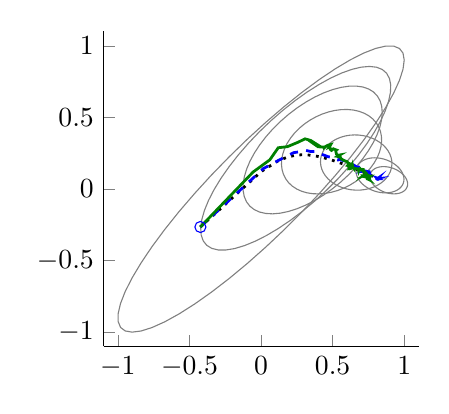
\begin{tikzpicture}

\begin{axis}[%
width=4cm,
height=4cm,
scale only axis,
xmin=-1.1,
xmax=1.1,
ymin=-1.1,
ymax=1.1,
axis x line*=bottom,
axis y line*=left
]
\addplot [
color=gray,
solid,
forget plot
]
table[row sep=crcr]{
-0.223606797749979 0.223606797749979\\
-0.0971317493977469 0.3464102286651\\
0.0309381995942439 0.463525613202567\\
0.15850014420423 0.573029919986106\\
0.283459520828355 0.67312509132574\\
0.403764499957141 0.762167567275353\\
0.517439677159302 0.838695272841565\\
0.6226185091679 0.9014516252147\\
0.717573962469178 0.949406166823786\\
0.800746871145116 0.981771485421374\\
0.870771538334692 0.998016143370882\\
0.926498160938592 0.997873403837886\\
0.967011709354304 0.98134561060157\\
0.991646952236901 0.948704149569941\\
0.999999379579327 0.900484992630715\\
0.991931844755535 0.837479897007744\\
0.967576816464294 0.760723404629287\\
0.927334203596814 0.671475854978151\\
0.871864788743812 0.571202690352226\\
0.80207937816364 0.461550393342469\\
0.719123846368702 0.344319451634276\\
0.624360320897642 0.221434794049475\\
0.519344816218816 0.0949141832682765\\
0.405801684015738 -0.0331649157781435\\
0.285595299380116 -0.16069944782438\\
0.16069944782438 -0.285595299380116\\
0.0331649157781437 -0.405801684015738\\
-0.0949141832682758 -0.519344816218815\\
-0.221434794049475 -0.624360320897642\\
-0.344319451634276 -0.719123846368702\\
-0.461550393342468 -0.80207937816364\\
-0.571202690352226 -0.871864788743812\\
-0.671475854978151 -0.927334203596814\\
-0.760723404629287 -0.967576816464294\\
-0.837479897007744 -0.991931844755535\\
-0.900484992630715 -0.999999379579327\\
-0.948704149569941 -0.991646952236901\\
-0.98134561060157 -0.967011709354304\\
-0.997873403837885 -0.926498160938592\\
-0.998016143370882 -0.870771538334693\\
-0.981771485421374 -0.800746871145116\\
-0.949406166823786 -0.717573962469179\\
-0.9014516252147 -0.6226185091679\\
-0.838695272841565 -0.517439677159303\\
-0.762167567275354 -0.403764499957142\\
-0.67312509132574 -0.283459520828355\\
-0.573029919986107 -0.15850014420423\\
-0.463525613202568 -0.030938199594244\\
-0.3464102286651 0.0971317493977463\\
-0.223606797749979 0.223606797749979\\
};
\addplot [
color=gray,
solid,
forget plot
]
table[row sep=crcr]{
0.456644734974626 -0.00969667801110813\\
0.374525791747298 -0.0847524663966239\\
0.29023584064942 -0.154897876594885\\
0.205158920347698 -0.218981122909709\\
0.120691991521408 -0.275949960208286\\
0.0382219988066626 -0.32486896175716\\
-0.0408969027961669 -0.364934878903337\\
-0.115365583110123 -0.395489830394961\\
-0.183961268463248 -0.416032104773275\\
-0.245557619598473 -0.426224398460909\\
-0.299143226133082 -0.425899354277293\\
-0.34383821388923 -0.415062309438937\\
-0.378908692403621 -0.39389120792248\\
-0.403778805388624 -0.362733678629514\\
-0.418040186276597 -0.322101327329635\\
-0.421458663587637 -0.272661336107845\\
-0.413978106018804 -0.215225508253162\\
-0.395721344118569 -0.150736938471062\\
-0.366988153412597 -0.0802545272944838\\
-0.32825033209791 -0.00493559396635573\\
-0.280143954129528 0.0739831267103794\\
-0.22345892490372 0.155205791524035\\
-0.159126011033233 0.237398726563892\\
-0.0882015571852386 0.319212326108943\\
-0.0118501409311103 0.399303213116517\\
0.0686745495851089 0.476356297436182\\
0.152050301171367 0.549106369553656\\
0.236908086291666 0.616358875296055\\
0.321854542460349 0.677009530378385\\
0.405494851215599 0.730062452720971\\
0.486455641000016 0.774646514805675\\
0.563407537883621 0.810029647565661\\
0.635086993847036 0.835630860939227\\
0.700317034205027 0.851029783710564\\
0.758026583498297 0.855973565993492\\
0.807268052522917 0.850381031019605\\
0.847232897718858 0.834344008058559\\
0.877264897432889 0.808125824584009\\
0.896870927059986 0.772156982443763\\
0.90572905613571 0.727028089031354\\
0.903693834425533 0.673480159528957\\
0.89079868021367 0.61239244945859\\
0.867255331575774 0.544768017330746\\
0.833450369645588 0.471717254451388\\
0.789938870963417 0.394439652327396\\
0.737435293134682 0.314204107049191\\
0.676801743455792 0.232328084052011\\
0.609033823136167 0.150155985369885\\
0.535244279553913 0.0690370745914021\\
0.456644734974626 -0.00969667801110799\\
};
\addplot [
color=gray,
solid,
forget plot
]
table[row sep=crcr]{
0.555425913311706 0.0472716755806835\\
0.496875664164754 -0.000161114180422195\\
0.436082271470401 -0.0431122116313219\\
0.374043961055967 -0.080876360939319\\
0.311779400263313 -0.112833475816823\\
0.250310971459259 -0.138458821321046\\
0.19064798454538 -0.157331629987261\\
0.133770104117331 -0.169142010818935\\
0.0806112633992654 -0.173696037689328\\
0.0320443290861189 -0.17091893360313\\
-0.011133231103392 -0.160856298532661\\
-0.0482124428246635 -0.14367336066758\\
-0.0785844664463428 -0.119652263372584\\
-0.101750594180242 -0.0891874324011575\\
-0.117330438849432 -0.0527790994356063\\
-0.125068179835172 -0.0110250882966617\\
-0.1248367636444 0.0353890013071266\\
-0.116639990124569 0.0857010513076516\\
-0.100612450070262 0.139084939234856\\
-0.0770173152460673 0.194664103124852\\
-0.0462420171134739 0.251525934643136\\
-0.00879188521699059 0.308736764088206\\
0.0347181503130071 0.365357191222255\\
0.0835736558960169 0.420457510197096\\
0.136972425481049 0.473132975298494\\
0.194037652747805 0.522518656845776\\
0.25383232824222 0.567803643313276\\
0.315374625045786 0.608244356475168\\
0.37765402034642 0.643176760939379\\
0.43964788819509 0.672027267590364\\
0.500338290995636 0.69432215190653\\
0.558728694011948 0.70969533250378\\
0.613860328440789 0.717894382181722\\
0.664827934369033 0.718784672771319\\
0.710794625116414 0.712351585725704\\
0.751005628891678 0.698700752156313\\
0.784800682124529 0.678056318372958\\
0.811624870975197 0.650757265407615\\
0.831037743004349 0.617251842955253\\
0.842720539389965 0.578090209126232\\
0.84648142893838 0.533915396865341\\
0.842258657947186 0.485452755368628\\
0.830121564199313 0.433498039869645\\
0.810269438438553 0.37890434536052\\
0.783028252021056 0.32256809879577\\
0.748845304474674 0.265414339786486\\
0.70828187885308 0.208381531475502\\
0.662004025483545 0.152406150998526\\
0.610771625438975 0.0984073125554682\\
0.555425913311706 0.0472716755806835\\
};
\addplot [
color=gray,
solid,
forget plot
]
table[row sep=crcr]{
0.622566809757817 0.028178664915152\\
0.57997101017793 0.00683114875754098\\
0.535938700569085 -0.0103515278383001\\
0.49119289023772 -0.0230872257977082\\
0.446468304152411 -0.0311668253122872\\
0.402499318780202 -0.0344576595813803\\
0.360007903645315 -0.0329056931972691\\
0.319691766609527 -0.0265364094050742\\
0.282212897528365 -0.0154543916685752\\
0.248186698395984 0.000158393587373684\\
0.218171878461432 0.0200455848605084\\
0.192661280238229 0.0438806350199351\\
0.172073787043923 0.0712721732009917\\
0.156747444947591 0.101770431104025\\
0.146933912062736 0.134874628177437\\
0.142794326328017 0.170041194420498\\
0.144396659626754 0.206692695787728\\
0.15171460169048 0.244227315639963\\
0.164627992112824 0.28202873655693\\
0.182924793380061 0.319476260252249\\
0.206304572521226 0.355954999422136\\
0.234383434209189 0.390865974177929\\
0.266700324311316 0.423635947279306\\
0.30272460038558 0.453726836673916\\
0.341864744814784 0.480644550789807\\
0.38347807750949 0.503947101505377\\
0.426881308697314 0.523251861582109\\
0.471361758522097 0.538241847393254\\
0.516189059227446 0.548670923786212\\
0.560627147775096 0.554367845614938\\
0.603946351979653 0.555239069580505\\
0.645435371705701 0.551270290209484\\
0.684412958396364 0.542526674749424\\
0.720239101155777 0.52915179312445\\
0.752325535710295 0.511365260521075\\
0.780145403691611 0.489459131312911\\
0.803241903636595 0.463793103535929\\
0.821235791654686 0.43478861265665\\
0.833831608602094 0.402921911613442\\
0.840822531512776 0.368716250756429\\
0.84209376962581 0.332733286091218\\
0.837624449246526 0.295563856902809\\
0.827487956491991 0.257818284190871\\
0.811850732292997 0.220116349215802\\
0.790969539438576 0.183077116707566\\
0.765187246538105 0.147308769839943\\
0.734927198128222 0.113398623879631\\
0.700686263367232 0.0819034824858006\\
0.663026677457268 0.0533404950094091\\
0.622566809757817 0.0281786649151521\\
};
\addplot [
color=gray,
solid,
forget plot
]
table[row sep=crcr]{
0.914082088679572 0.169354942779576\\
0.913540227303751 0.19408814269724\\
0.908912819009833 0.218665696555725\\
0.900275845714073 0.242684041600158\\
0.887771126279205 0.265748797268932\\
0.871603987852639 0.287481240911626\\
0.852039894400373 0.307524526404453\\
0.829400087796016 0.325549543553746\\
0.8040563130381 0.341260322076243\\
0.776424714207483 0.354398891422953\\
0.746959001393047 0.364749516648437\\
0.716143000784581 0.372142240772653\\
0.684482710260123 0.376455675469862\\
0.652497990914788 0.377618994261588\\
0.620714030955961 0.375613095485434\\
0.589652722127451 0.370470915943846\\
0.559824090261486 0.362276890082735\\
0.531717920668648 0.351165563580205\\
0.505795715876614 0.337319384110237\\
0.482483117771412 0.32096570555693\\
0.462162918569417 0.302373054870007\\
0.445168775379744 0.281846722859727\\
0.431779731563739 0.259723751330217\\
0.422215634850701 0.236367398862369\\
0.416633527444244 0.212161176117984\\
0.415125067393656 0.187502548605307\\
0.417715023571264 0.162796410306372\\
0.424360868968236 0.13844843532901\\
0.434953478986887 0.114858416749212\\
0.449318923263559 0.0924137020198785\\
0.467221321600384 0.0714828327363465\\
0.48836671711161 0.0524094931935867\\
0.512407902987538 0.0355068670995803\\
0.53895012362074 0.0210524951074926\\
0.567557556482218 0.00928371760582095\\
0.597760468315282 0.000393777595777522\\
0.629062928142637 -0.00547135235344862\\
0.660950950439322 -0.00821536697024131\\
0.692900934760816 -0.00779320961045532\\
0.724388263247867 -0.00421181208626706\\
0.75489591483723 0.00247001915398939\\
0.783922954733238 0.0121425686260781\\
0.810992759743295 0.0246470133350796\\
0.83566084441752 0.0397780306445759\\
0.857522159487549 0.0572871696686647\\
0.87621774276432 0.0768869308286371\\
0.891440613287296 0.0982554865881104\\
0.902940811943349 0.12104196585228\\
0.910529505788486 0.144872215261594\\
0.914082088679572 0.169354942779576\\
};
\addplot [
color=gray,
solid,
forget plot
]
table[row sep=crcr]{
0.795978184921688 -0.015786231265185\\
0.775374058911572 -0.00823025761854718\\
0.755687875383625 0.00102425255066693\\
0.737242880927121 0.0118253404413336\\
0.720341941841098 0.0239956524889001\\
0.705262571078097 0.0373353525060121\\
0.692252371489153 0.0516254029871843\\
0.681524970191831 0.0666311616985858\\
0.673256510818858 0.0821062344970318\\
0.667582761244544 0.0977965211150035\\
0.664596884280041 0.113444387480015\\
0.664347907942556 0.128792896058962\\
0.666839920416667 0.143590024765309\\
0.672032002926446 0.157592805154789\\
0.679838901620624 0.170571311960532\\
0.690132427438476 0.182312438459599\\
0.702743560970654 0.192623395679477\\
0.717465227753211 0.201334877987676\\
0.734055698424582 0.208303843085539\\
0.752242557915011 0.213415860758825\\
0.771727178494467 0.216586991818668\\
0.792189623231717 0.217765166380737\\
0.813293899349891 0.216931038851295\\
0.834693475218588 0.214098305581314\\
0.856036970393665 0.209313479972772\\
0.876973925274423 0.202655128729879\\
0.897160555640551 0.194232581795962\\
0.916265397579528 0.184184137158822\\
0.933974750114897 0.172674790001598\\
0.949997826167629 0.159893523486416\\
0.964071527271921 0.146050205656101\\
0.975964763644727 0.131372143406705\\
0.985482248673613 0.116100350114568\\
0.992467705517531 0.100485588203335\\
0.996806433168224 0.0847842516318938\\
0.998427189837622 0.0692541559126621\\
0.997303362746019 0.0541503047879964\\
0.99345340510319 0.0397207030757953\\
0.986940533107192 0.0262022844372453\\
0.977871687936142 0.0138170209326543\\
0.966395779777027 0.00276827824635879\\
0.952701242724551 -0.00676252357219119\\
0.937012940698509 -0.0146188890206284\\
0.919588475184443 -0.0206718167954904\\
0.900713955424368 -0.0248219179900562\\
0.880699300510929 -0.0270010480574468\\
0.859873150524472 -0.0271734257422009\\
0.838577470272004 -0.0253362206075004\\
0.817161934234519 -0.0215195995108649\\
0.795978184921688 -0.015786231265185\\
};
\addplot [
color=gray,
solid,
forget plot
]
table[row sep=crcr]{
1.0205476199241 0.0146304111508795\\
1.02334270847121 0.0256309088856638\\
1.02398659147348 0.037213622368035\\
1.02246869638982 0.0491883637628339\\
1.01881394701554 0.0613585081474175\\
1.01308235423431 0.0735242220874528\\
1.00536803064115 0.0854857448963837\\
0.995797645216192 0.0970466687003816\\
0.984528343423516 0.108017163450204\\
0.971745166887005 0.118217093925354\\
0.957658015011978 0.127478977549423\\
0.942498198442762 0.135650734449362\\
0.926514640948309 0.142598184602794\\
0.909969792100788 0.148207251070272\\
0.893135317860868 0.152385833135472\\
0.876287639830155 0.155065318596405\\
0.859703396416133 0.156201710375883\\
0.843654900437165 0.155776348952303\\
0.828405667753541 0.15379621874848\\
0.814206090344339 0.150293833447618\\
0.801289324878047 0.145326702119528\\
0.789867464286521 0.138976384923294\\
0.780128055204899 0.131347153891713\\
0.772231018461039 0.122564280787404\\
0.766306023179952 0.112771980143922\\
0.762450357620347 0.102131041267112\\
0.760727331704116 0.0908161880791451\\
0.761165237469171 0.0790132101565527\\
0.763756884514953 0.0669159120705125\\
0.768459718068622 0.0547229311211495\\
0.775196517733244 0.042634475718559\\
0.783856665444573 0.0308490379662483\\
0.794297961816613 0.0195601344262841\\
0.806348961051601 0.00895312858269419\\
0.819811786075265 -0.000797812821816249\\
0.834465377672916 -0.00953257959896436\\
0.850069124275642 -0.0171077471197552\\
0.866366812795615 -0.0233989313429241\\
0.883090835637911 -0.0283028311974558\\
0.89996658480982 -0.0317389247833146\\
0.916716960976494 -0.0336507915388166\\
0.933066923424366 -0.0340070386646928\\
0.94874800622206 -0.0328018165929853\\
0.963502726423567 -0.0300549150367915\\
0.977088811931092 -0.0258114380437218\\
0.98928317959621 -0.0201410633886851\\
0.999885598238992 -0.0131368984667513\\
1.00872197643844 -0.00491395147229781\\
1.01564722110882 0.00439275703236196\\
1.0205476199241 0.0146304111508795\\
};
\addplot [
color=blue,
only marks,
mark=o,
mark options={solid},
forget plot
]
table[row sep=crcr]{
-0.423658160306465 -0.265544277298046\\
};
\addplot [
color=black,
dotted,
line width=1.0pt,
forget plot
]
table[row sep=crcr]{
-0.423658160306465 -0.265544277298046\\
0.00242150590264467 0.122787079650492\\
0.119860995112355 0.196913937568555\\
0.188006844724955 0.22385638260482\\
0.237332543640276 0.234725527504476\\
0.276755147380961 0.238387931243253\\
0.309972822367975 0.238350330890813\\
0.33885921377211 0.236269678518997\\
0.364498667373003 0.233020943752307\\
0.387581375752828 0.22910191644929\\
0.408578923000339 0.224810830155441\\
0.427831457028349 0.220332911490062\\
0.445594872292462 0.215786008549946\\
0.462068175600546 0.211246163927359\\
0.477410287840286 0.206762662475913\\
0.491750864135096 0.202367241766044\\
0.505197550439098 0.198079914846599\\
0.517841022558555 0.193912751104659\\
0.52975859203918 0.189872386452409\\
0.541016854716125 0.185961720987173\\
0.551673680834573 0.18218108483713\\
0.561779740466219 0.178529048868203\\
0.571379693321013 0.175002994085654\\
0.58051313116453 0.171599514599526\\
0.589215334487547 0.16831470429785\\
0.597517887398241 0.165144361355447\\
0.605449182685881 0.162084134138763\\
0.613034840664175 0.159129624978834\\
0.620298059508905 0.156276463458587\\
0.627259910569584 0.153520357530856\\
0.633939589044394 0.150857128457993\\
0.640354628120062 0.148282733921915\\
0.646521082962575 0.145793282482559\\
0.652453689642047 0.143385041720243\\
0.658166003074998 0.141054441786378\\
0.663670517291457 0.138798075640508\\
0.668978770726548 0.136612696923383\\
0.674101438755884 0.13449521617294\\
0.679048415311284 0.132442695909547\\
0.683828885105843 0.130452344982138\\
0.688451387748645 0.128521512465838\\
0.692923874826822 0.126647681325779\\
0.697253760866618 0.124828462004642\\
0.70144796894823 0.123061586048288\\
0.705512971635701 0.121344899851306\\
0.709454827788602 0.119676358579702\\
0.713279215743047 0.118054020309453\\
0.716991463282974 0.116476040405716\\
0.720596574766369 0.114940666157084\\
0.724099255723382 0.113446231671519\\
0.727503935202617 0.111991153034902\\
0.73081478610719 0.110573923729004\\
0.734035743732302 0.109193110302682\\
0.737170522690515 0.107847348288089\\
0.740222632388734 0.106535338352286\\
0.743195391201804 0.105255842673812\\
0.746091939470981 0.104007681533272\\
0.748915251441087 0.102789730106862\\
0.751668146237511 0.101600915451779\\
0.754353297973212 0.100440213672642\\
0.756973245066157 0.0993066472583866\\
0.75953039883915 0.0981992825794537\\
0.762027051466476 0.0971172275355389\\
0.764465383325214 0.0960596293446205\\
0.766847469803174 0.0950256724644703\\
0.769175287610265 0.0940145766383234\\
0.771450720635486 0.0930255950568635\\
0.773675565387618 0.0920580126291417\\
0.775851536054101 0.0911111443554959\\
0.777980269209262 0.0901843337959739\\
0.780063328200204 0.0892769516281689\\
0.782102207236029 0.0883883942887737\\
0.784098335203756 0.0875180826935251\\
0.786053079232178 0.0866654610305641\\
0.787967748023034 0.0858299956225609\\
0.789843594967175 0.0850111738532671\\
0.791681821061853 0.0842085031544414\\
0.793483577643902 0.0834215100493708\\
0.795249968952332 0.0826497392494552\\
0.7969820545327 0.0818927528005651\\
0.798680851494636 0.0811501292760977\\
0.800347336632936 0.080421463013864\\
0.801982448421829 0.0797063633941279\\
0.803587088891209 0.0790044541562991\\
0.805162125392979 0.0783153727519431\\
0.806708392264973 0.0776387697319298\\
0.80822669239937 0.0769743081656825\\
0.809717798721966 0.0763216630906227\\
0.811182455588192 0.0756805209900316\\
0.812621380101344 0.0750505792976646\\
0.814035263358031 0.07443154592756\\
0.81542477162554 0.0738231388275862\\
0.816790547455432 0.0732250855553643\\
0.81813321073739 0.0726371228752879\\
0.819453359697028 0.0720589963754441\\
0.820751571841154 0.0714904601033156\\
0.822028404853678 0.070931276219213\\
0.823284397445168 0.0703812146664506\\
0.824520070158853 0.0698400528573428\\
0.825735926135646 0.0693075753741537\\
0.826932451840631 0.0687835736841832\\
};
\addplot [
color=blue,
dashed,
line width=1.0pt,
forget plot
]
table[row sep=crcr]{
-0.423658160306465 -0.265544277298046\\
0.0150764734847799 0.141713645028666\\
0.128266448251792 0.203061419228372\\
0.22669657170916 0.253535394239362\\
0.276984522465355 0.261006022043223\\
0.314160741859687 0.269650622899764\\
0.347821518442704 0.261207424958875\\
0.378195026465508 0.262517933514043\\
0.403124906907465 0.25388294243401\\
0.418451275881427 0.244472637319418\\
0.439771613306922 0.236075699622215\\
0.457446033461072 0.229817673462225\\
0.470032041223307 0.224368357039128\\
0.491317179742705 0.223780708510906\\
0.500003115472698 0.214399545231926\\
0.510240222954932 0.210945973885522\\
0.518283740368447 0.206410615746778\\
0.537532706535306 0.202242328096033\\
0.544284701549024 0.205948198993329\\
0.554302655300813 0.204588987811089\\
0.558552231168685 0.202072651240517\\
0.574335222619425 0.198786965164456\\
0.580249746446143 0.197109623497662\\
0.590174871682169 0.189637286960168\\
0.601160310406428 0.193743972514359\\
0.609171759818325 0.184341134243007\\
0.620281677824765 0.178174882673582\\
0.628884799103075 0.173126404023472\\
0.642402014841729 0.169133561500065\\
0.654311318750228 0.162843724927911\\
0.666329303265718 0.154246854556376\\
0.682765042033113 0.153180031510408\\
0.686800080206799 0.149885830747641\\
0.695221437779026 0.141711532082627\\
0.694804262768244 0.141000393817934\\
0.695013585666167 0.141902583100789\\
0.700129999401421 0.138936953160248\\
0.702333756902603 0.134448150740603\\
0.700009325319683 0.135249005050468\\
0.704666564242927 0.131218554528193\\
0.706390968286814 0.132734911121016\\
0.709946020328424 0.128802249694482\\
0.719419507674847 0.127246315289755\\
0.722642272155939 0.127345774869413\\
0.721809839856199 0.126715450299851\\
0.725148241023072 0.125431226578078\\
0.724449245144119 0.125139770483216\\
0.729507139516062 0.125706382584547\\
0.735055750532655 0.123736664050632\\
0.737503370711441 0.122274940478969\\
0.745300490304115 0.121349546245666\\
0.749295460965084 0.117506133931847\\
0.752634599553002 0.117132929282051\\
0.755183319264509 0.115425050709325\\
0.755655853464857 0.113227657699763\\
0.758028539676943 0.111343587244499\\
0.757295116784256 0.113715590494597\\
0.755826792170151 0.111888078748728\\
0.757662841985657 0.111615130214658\\
0.757822207564221 0.109098462894216\\
0.761292304123277 0.10167333198567\\
0.760586903991302 0.102740448720043\\
0.764023718942325 0.0984064214066678\\
0.766719011053783 0.0973923522181611\\
0.76961536445881 0.0971315362800118\\
0.778073805626339 0.0910693389405452\\
0.783473762085921 0.0865437273795604\\
0.787238214973759 0.0822323217366929\\
0.789343424791777 0.08259015816049\\
0.794259185396647 0.0801776890521058\\
0.792512714679819 0.081463090579629\\
0.796719722610988 0.0814962705039133\\
0.801003635406211 0.0808568021145043\\
0.806411873120944 0.0766775287254546\\
0.810618242255894 0.0772197090558023\\
0.805839159499941 0.0782065097389542\\
0.808065627761535 0.0756642096008819\\
0.812156222221671 0.0734156369277934\\
0.815770119780439 0.0734435499205703\\
0.816756666417879 0.0745972461736448\\
0.815294717032733 0.0735464680265237\\
0.814494774658996 0.0722875185100304\\
0.816703929578228 0.0722415452207195\\
0.812692778557632 0.0741879839787607\\
0.814002603911476 0.0710724194508479\\
0.820501093627315 0.0718321762859395\\
0.818647899243582 0.0711293118976905\\
0.819011976553334 0.0733112266091904\\
0.82200990231907 0.0726475207041034\\
0.82202669626064 0.0691426478181728\\
0.82349899646827 0.0694836750869472\\
0.823783637607849 0.0688108694594397\\
0.826880909090058 0.0685441765496974\\
0.827545452125074 0.0679062463922276\\
0.826943669030874 0.0674114110356461\\
0.82745608819192 0.0675230320209754\\
0.834046637327064 0.0679194615839197\\
0.832375493903718 0.0707538789032289\\
0.831490871272005 0.0709659999278264\\
0.831660602192682 0.0689006934969698\\
0.828829415415717 0.0698164321398679\\
};
\addplot [
color=green!50!black,
solid,
line width=1.0pt,
forget plot
]
table[row sep=crcr]{
-0.423658160306465 -0.265544277298046\\
-0.0549619814773591 0.118905560965915\\
0.0611900825861636 0.203436753119323\\
0.120109030303461 0.287894077984681\\
0.184914785888709 0.295752039420244\\
0.258056733824465 0.32631445172747\\
0.307562099907215 0.350034232288437\\
0.346474534696256 0.339153890567492\\
0.383539193743067 0.315737286050682\\
0.355931520963756 0.324350689858913\\
0.397483596186667 0.295193766511885\\
0.42160539285663 0.292692105062653\\
0.436539752075579 0.293636432715814\\
0.439240287549775 0.28734870752013\\
0.45483391205266 0.299050655909251\\
0.465827688634448 0.305178168644249\\
0.487123661934733 0.310835883476853\\
0.478326164058298 0.295864544264346\\
0.48179786392265 0.29777218887497\\
0.483240802146808 0.277043008568191\\
0.49222239974003 0.269592894710355\\
0.505132748333046 0.280406737967897\\
0.526241657930929 0.272337269125332\\
0.521063838650468 0.268730671114344\\
0.521929060573914 0.26595276421186\\
0.526455207115231 0.24452964915957\\
0.536813902515015 0.235196942231384\\
0.550790212208966 0.237689137012003\\
0.533795508169064 0.227429084719918\\
0.553130903549037 0.22426921659041\\
0.559228100048614 0.210245915387877\\
0.583184021124399 0.196892370434251\\
0.602789764235752 0.190688210814037\\
0.605910075020372 0.181043904535424\\
0.615367888791609 0.178347559098766\\
0.625524290857247 0.172944316175946\\
0.61252301838854 0.169359695785367\\
0.606335949811397 0.163513821824845\\
0.617714299649339 0.160639287931992\\
0.634139790657078 0.156547337341809\\
0.637526304424482 0.149979800156245\\
0.629034318689475 0.168177836518465\\
0.621918753545596 0.160401808334733\\
0.615350304501684 0.14191045391587\\
0.623998664699659 0.14312609088017\\
0.623413471042154 0.148054993164301\\
0.620078683167653 0.144487005575743\\
0.612786167829917 0.152775245792342\\
0.615782667214696 0.149574545211305\\
0.620183039053663 0.153644365832568\\
0.622117976017808 0.156453812622943\\
0.635256479971316 0.156014726760737\\
0.642712610390725 0.147535027230091\\
0.640339563568981 0.157877258361172\\
0.638736857164934 0.148794419678204\\
0.657020679494355 0.1441900339601\\
0.672262214796502 0.140033157968078\\
0.674158209282595 0.140499702518238\\
0.682265172645078 0.130439010286057\\
0.68136474498082 0.127410439357832\\
0.679543455406662 0.134539893519713\\
0.685954363558128 0.13267623202126\\
0.686999377926314 0.141661895787656\\
0.683750391259635 0.140709003931584\\
0.683837737346897 0.138175699198264\\
0.705805494997607 0.137005164528778\\
0.703856483125101 0.134476368547535\\
0.711762564385371 0.125299162432966\\
0.716320152850343 0.130460221181414\\
0.721973251206943 0.123262838037093\\
0.724617414621529 0.121780762986902\\
0.728972169917787 0.127867252699477\\
0.726321971162613 0.123417117163446\\
0.730291169468817 0.110756619933168\\
0.732778540569512 0.109336727810331\\
0.71939922351489 0.09666849140913\\
0.724571867219492 0.0993930159422993\\
0.7304649705255 0.0987085850835294\\
0.74004773871398 0.0963032494376266\\
0.725864838562941 0.0944192197513796\\
0.732554899407043 0.0977490672468534\\
0.736100629131383 0.0951499722647115\\
0.731167153556259 0.0941590842633866\\
0.729505787845459 0.0871793520300228\\
0.732001511005409 0.0833510725177911\\
0.714569519023427 0.0872609151851703\\
0.717406851231904 0.0905376992739934\\
0.715648115959882 0.0920291538214647\\
0.724208891560132 0.0923151040681435\\
0.740820704133793 0.0867245380769161\\
0.744416546861374 0.0810664401026933\\
0.758115927612689 0.0745443682255588\\
0.759110081304389 0.0685067070430162\\
0.749894291964036 0.0702345639255953\\
0.754982717939339 0.0646159279017507\\
0.742460324108607 0.0711199205373331\\
0.741651052874918 0.0730930395131353\\
0.749651747703426 0.0758540715647245\\
0.747658963283614 0.0741493804225888\\
0.743074704301771 0.0732882500238929\\
0.743427204107473 0.0764487169924193\\
};
\end{axis}
\end{tikzpicture}% }
\subfloat[]{ % This file was created by matlab2tikz v0.4.4 running on MATLAB 7.13.
% Copyright (c) 2008--2013, Nico Schlömer <nico.schloemer@gmail.com>
% All rights reserved.
% 
% The latest updates can be retrieved from
%   http://www.mathworks.com/matlabcentral/fileexchange/22022-matlab2tikz
% where you can also make suggestions and rate matlab2tikz.
% 
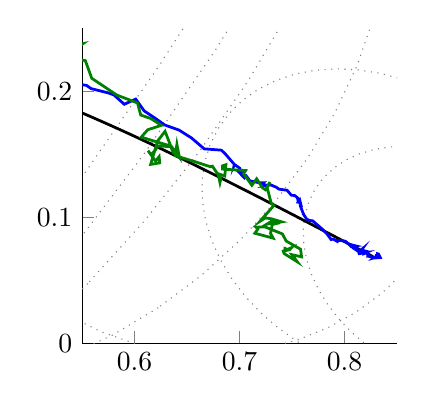
\begin{tikzpicture}

\begin{axis}[%
width=4cm,
height=4cm,
scale only axis,
xmin=0.55,
xmax=0.85,
ymin=0,
ymax=0.25,
axis x line*=bottom,
axis y line*=left
]
\addplot [
color=gray,
dotted,
forget plot
]
table[row sep=crcr]{
-0.223606797749979 0.223606797749979\\
-0.0971317493977469 0.3464102286651\\
0.0309381995942439 0.463525613202567\\
0.15850014420423 0.573029919986106\\
0.283459520828355 0.67312509132574\\
0.403764499957141 0.762167567275353\\
0.517439677159302 0.838695272841565\\
0.6226185091679 0.9014516252147\\
0.717573962469178 0.949406166823786\\
0.800746871145116 0.981771485421374\\
0.870771538334692 0.998016143370882\\
0.926498160938592 0.997873403837886\\
0.967011709354304 0.98134561060157\\
0.991646952236901 0.948704149569941\\
0.999999379579327 0.900484992630715\\
0.991931844755535 0.837479897007744\\
0.967576816464294 0.760723404629287\\
0.927334203596814 0.671475854978151\\
0.871864788743812 0.571202690352226\\
0.80207937816364 0.461550393342469\\
0.719123846368702 0.344319451634276\\
0.624360320897642 0.221434794049475\\
0.519344816218816 0.0949141832682765\\
0.405801684015738 -0.0331649157781435\\
0.285595299380116 -0.16069944782438\\
0.16069944782438 -0.285595299380116\\
0.0331649157781437 -0.405801684015738\\
-0.0949141832682758 -0.519344816218815\\
-0.221434794049475 -0.624360320897642\\
-0.344319451634276 -0.719123846368702\\
-0.461550393342468 -0.80207937816364\\
-0.571202690352226 -0.871864788743812\\
-0.671475854978151 -0.927334203596814\\
-0.760723404629287 -0.967576816464294\\
-0.837479897007744 -0.991931844755535\\
-0.900484992630715 -0.999999379579327\\
-0.948704149569941 -0.991646952236901\\
-0.98134561060157 -0.967011709354304\\
-0.997873403837885 -0.926498160938592\\
-0.998016143370882 -0.870771538334693\\
-0.981771485421374 -0.800746871145116\\
-0.949406166823786 -0.717573962469179\\
-0.9014516252147 -0.6226185091679\\
-0.838695272841565 -0.517439677159303\\
-0.762167567275354 -0.403764499957142\\
-0.67312509132574 -0.283459520828355\\
-0.573029919986107 -0.15850014420423\\
-0.463525613202568 -0.030938199594244\\
-0.3464102286651 0.0971317493977463\\
-0.223606797749979 0.223606797749979\\
};
\addplot [
color=gray,
dotted,
forget plot
]
table[row sep=crcr]{
0.456644734974626 -0.00969667801110813\\
0.374525791747298 -0.0847524663966239\\
0.29023584064942 -0.154897876594885\\
0.205158920347698 -0.218981122909709\\
0.120691991521408 -0.275949960208286\\
0.0382219988066626 -0.32486896175716\\
-0.0408969027961669 -0.364934878903337\\
-0.115365583110123 -0.395489830394961\\
-0.183961268463248 -0.416032104773275\\
-0.245557619598473 -0.426224398460909\\
-0.299143226133082 -0.425899354277293\\
-0.34383821388923 -0.415062309438937\\
-0.378908692403621 -0.39389120792248\\
-0.403778805388624 -0.362733678629514\\
-0.418040186276597 -0.322101327329635\\
-0.421458663587637 -0.272661336107845\\
-0.413978106018804 -0.215225508253162\\
-0.395721344118569 -0.150736938471062\\
-0.366988153412597 -0.0802545272944838\\
-0.32825033209791 -0.00493559396635573\\
-0.280143954129528 0.0739831267103794\\
-0.22345892490372 0.155205791524035\\
-0.159126011033233 0.237398726563892\\
-0.0882015571852386 0.319212326108943\\
-0.0118501409311103 0.399303213116517\\
0.0686745495851089 0.476356297436182\\
0.152050301171367 0.549106369553656\\
0.236908086291666 0.616358875296055\\
0.321854542460349 0.677009530378385\\
0.405494851215599 0.730062452720971\\
0.486455641000016 0.774646514805675\\
0.563407537883621 0.810029647565661\\
0.635086993847036 0.835630860939227\\
0.700317034205027 0.851029783710564\\
0.758026583498297 0.855973565993492\\
0.807268052522917 0.850381031019605\\
0.847232897718858 0.834344008058559\\
0.877264897432889 0.808125824584009\\
0.896870927059986 0.772156982443763\\
0.90572905613571 0.727028089031354\\
0.903693834425533 0.673480159528957\\
0.89079868021367 0.61239244945859\\
0.867255331575774 0.544768017330746\\
0.833450369645588 0.471717254451388\\
0.789938870963417 0.394439652327396\\
0.737435293134682 0.314204107049191\\
0.676801743455792 0.232328084052011\\
0.609033823136167 0.150155985369885\\
0.535244279553913 0.0690370745914021\\
0.456644734974626 -0.00969667801110799\\
};
\addplot [
color=gray,
dotted,
forget plot
]
table[row sep=crcr]{
0.555425913311706 0.0472716755806835\\
0.496875664164754 -0.000161114180422195\\
0.436082271470401 -0.0431122116313219\\
0.374043961055967 -0.080876360939319\\
0.311779400263313 -0.112833475816823\\
0.250310971459259 -0.138458821321046\\
0.19064798454538 -0.157331629987261\\
0.133770104117331 -0.169142010818935\\
0.0806112633992654 -0.173696037689328\\
0.0320443290861189 -0.17091893360313\\
-0.011133231103392 -0.160856298532661\\
-0.0482124428246635 -0.14367336066758\\
-0.0785844664463428 -0.119652263372584\\
-0.101750594180242 -0.0891874324011575\\
-0.117330438849432 -0.0527790994356063\\
-0.125068179835172 -0.0110250882966617\\
-0.1248367636444 0.0353890013071266\\
-0.116639990124569 0.0857010513076516\\
-0.100612450070262 0.139084939234856\\
-0.0770173152460673 0.194664103124852\\
-0.0462420171134739 0.251525934643136\\
-0.00879188521699059 0.308736764088206\\
0.0347181503130071 0.365357191222255\\
0.0835736558960169 0.420457510197096\\
0.136972425481049 0.473132975298494\\
0.194037652747805 0.522518656845776\\
0.25383232824222 0.567803643313276\\
0.315374625045786 0.608244356475168\\
0.37765402034642 0.643176760939379\\
0.43964788819509 0.672027267590364\\
0.500338290995636 0.69432215190653\\
0.558728694011948 0.70969533250378\\
0.613860328440789 0.717894382181722\\
0.664827934369033 0.718784672771319\\
0.710794625116414 0.712351585725704\\
0.751005628891678 0.698700752156313\\
0.784800682124529 0.678056318372958\\
0.811624870975197 0.650757265407615\\
0.831037743004349 0.617251842955253\\
0.842720539389965 0.578090209126232\\
0.84648142893838 0.533915396865341\\
0.842258657947186 0.485452755368628\\
0.830121564199313 0.433498039869645\\
0.810269438438553 0.37890434536052\\
0.783028252021056 0.32256809879577\\
0.748845304474674 0.265414339786486\\
0.70828187885308 0.208381531475502\\
0.662004025483545 0.152406150998526\\
0.610771625438975 0.0984073125554682\\
0.555425913311706 0.0472716755806835\\
};
\addplot [
color=gray,
dotted,
forget plot
]
table[row sep=crcr]{
0.622566809757817 0.028178664915152\\
0.57997101017793 0.00683114875754098\\
0.535938700569085 -0.0103515278383001\\
0.49119289023772 -0.0230872257977082\\
0.446468304152411 -0.0311668253122872\\
0.402499318780202 -0.0344576595813803\\
0.360007903645315 -0.0329056931972691\\
0.319691766609527 -0.0265364094050742\\
0.282212897528365 -0.0154543916685752\\
0.248186698395984 0.000158393587373684\\
0.218171878461432 0.0200455848605084\\
0.192661280238229 0.0438806350199351\\
0.172073787043923 0.0712721732009917\\
0.156747444947591 0.101770431104025\\
0.146933912062736 0.134874628177437\\
0.142794326328017 0.170041194420498\\
0.144396659626754 0.206692695787728\\
0.15171460169048 0.244227315639963\\
0.164627992112824 0.28202873655693\\
0.182924793380061 0.319476260252249\\
0.206304572521226 0.355954999422136\\
0.234383434209189 0.390865974177929\\
0.266700324311316 0.423635947279306\\
0.30272460038558 0.453726836673916\\
0.341864744814784 0.480644550789807\\
0.38347807750949 0.503947101505377\\
0.426881308697314 0.523251861582109\\
0.471361758522097 0.538241847393254\\
0.516189059227446 0.548670923786212\\
0.560627147775096 0.554367845614938\\
0.603946351979653 0.555239069580505\\
0.645435371705701 0.551270290209484\\
0.684412958396364 0.542526674749424\\
0.720239101155777 0.52915179312445\\
0.752325535710295 0.511365260521075\\
0.780145403691611 0.489459131312911\\
0.803241903636595 0.463793103535929\\
0.821235791654686 0.43478861265665\\
0.833831608602094 0.402921911613442\\
0.840822531512776 0.368716250756429\\
0.84209376962581 0.332733286091218\\
0.837624449246526 0.295563856902809\\
0.827487956491991 0.257818284190871\\
0.811850732292997 0.220116349215802\\
0.790969539438576 0.183077116707566\\
0.765187246538105 0.147308769839943\\
0.734927198128222 0.113398623879631\\
0.700686263367232 0.0819034824858006\\
0.663026677457268 0.0533404950094091\\
0.622566809757817 0.0281786649151521\\
};
\addplot [
color=gray,
dotted,
forget plot
]
table[row sep=crcr]{
0.914082088679572 0.169354942779576\\
0.913540227303751 0.19408814269724\\
0.908912819009833 0.218665696555725\\
0.900275845714073 0.242684041600158\\
0.887771126279205 0.265748797268932\\
0.871603987852639 0.287481240911626\\
0.852039894400373 0.307524526404453\\
0.829400087796016 0.325549543553746\\
0.8040563130381 0.341260322076243\\
0.776424714207483 0.354398891422953\\
0.746959001393047 0.364749516648437\\
0.716143000784581 0.372142240772653\\
0.684482710260123 0.376455675469862\\
0.652497990914788 0.377618994261588\\
0.620714030955961 0.375613095485434\\
0.589652722127451 0.370470915943846\\
0.559824090261486 0.362276890082735\\
0.531717920668648 0.351165563580205\\
0.505795715876614 0.337319384110237\\
0.482483117771412 0.32096570555693\\
0.462162918569417 0.302373054870007\\
0.445168775379744 0.281846722859727\\
0.431779731563739 0.259723751330217\\
0.422215634850701 0.236367398862369\\
0.416633527444244 0.212161176117984\\
0.415125067393656 0.187502548605307\\
0.417715023571264 0.162796410306372\\
0.424360868968236 0.13844843532901\\
0.434953478986887 0.114858416749212\\
0.449318923263559 0.0924137020198785\\
0.467221321600384 0.0714828327363465\\
0.48836671711161 0.0524094931935867\\
0.512407902987538 0.0355068670995803\\
0.53895012362074 0.0210524951074926\\
0.567557556482218 0.00928371760582095\\
0.597760468315282 0.000393777595777522\\
0.629062928142637 -0.00547135235344862\\
0.660950950439322 -0.00821536697024131\\
0.692900934760816 -0.00779320961045532\\
0.724388263247867 -0.00421181208626706\\
0.75489591483723 0.00247001915398939\\
0.783922954733238 0.0121425686260781\\
0.810992759743295 0.0246470133350796\\
0.83566084441752 0.0397780306445759\\
0.857522159487549 0.0572871696686647\\
0.87621774276432 0.0768869308286371\\
0.891440613287296 0.0982554865881104\\
0.902940811943349 0.12104196585228\\
0.910529505788486 0.144872215261594\\
0.914082088679572 0.169354942779576\\
};
\addplot [
color=gray,
dotted,
forget plot
]
table[row sep=crcr]{
0.795978184921688 -0.015786231265185\\
0.775374058911572 -0.00823025761854718\\
0.755687875383625 0.00102425255066693\\
0.737242880927121 0.0118253404413336\\
0.720341941841098 0.0239956524889001\\
0.705262571078097 0.0373353525060121\\
0.692252371489153 0.0516254029871843\\
0.681524970191831 0.0666311616985858\\
0.673256510818858 0.0821062344970318\\
0.667582761244544 0.0977965211150035\\
0.664596884280041 0.113444387480015\\
0.664347907942556 0.128792896058962\\
0.666839920416667 0.143590024765309\\
0.672032002926446 0.157592805154789\\
0.679838901620624 0.170571311960532\\
0.690132427438476 0.182312438459599\\
0.702743560970654 0.192623395679477\\
0.717465227753211 0.201334877987676\\
0.734055698424582 0.208303843085539\\
0.752242557915011 0.213415860758825\\
0.771727178494467 0.216586991818668\\
0.792189623231717 0.217765166380737\\
0.813293899349891 0.216931038851295\\
0.834693475218588 0.214098305581314\\
0.856036970393665 0.209313479972772\\
0.876973925274423 0.202655128729879\\
0.897160555640551 0.194232581795962\\
0.916265397579528 0.184184137158822\\
0.933974750114897 0.172674790001598\\
0.949997826167629 0.159893523486416\\
0.964071527271921 0.146050205656101\\
0.975964763644727 0.131372143406705\\
0.985482248673613 0.116100350114568\\
0.992467705517531 0.100485588203335\\
0.996806433168224 0.0847842516318938\\
0.998427189837622 0.0692541559126621\\
0.997303362746019 0.0541503047879964\\
0.99345340510319 0.0397207030757953\\
0.986940533107192 0.0262022844372453\\
0.977871687936142 0.0138170209326543\\
0.966395779777027 0.00276827824635879\\
0.952701242724551 -0.00676252357219119\\
0.937012940698509 -0.0146188890206284\\
0.919588475184443 -0.0206718167954904\\
0.900713955424368 -0.0248219179900562\\
0.880699300510929 -0.0270010480574468\\
0.859873150524472 -0.0271734257422009\\
0.838577470272004 -0.0253362206075004\\
0.817161934234519 -0.0215195995108649\\
0.795978184921688 -0.015786231265185\\
};
\addplot [
color=gray,
dotted,
forget plot
]
table[row sep=crcr]{
1.0205476199241 0.0146304111508795\\
1.02334270847121 0.0256309088856638\\
1.02398659147348 0.037213622368035\\
1.02246869638982 0.0491883637628339\\
1.01881394701554 0.0613585081474175\\
1.01308235423431 0.0735242220874528\\
1.00536803064115 0.0854857448963837\\
0.995797645216192 0.0970466687003816\\
0.984528343423516 0.108017163450204\\
0.971745166887005 0.118217093925354\\
0.957658015011978 0.127478977549423\\
0.942498198442762 0.135650734449362\\
0.926514640948309 0.142598184602794\\
0.909969792100788 0.148207251070272\\
0.893135317860868 0.152385833135472\\
0.876287639830155 0.155065318596405\\
0.859703396416133 0.156201710375883\\
0.843654900437165 0.155776348952303\\
0.828405667753541 0.15379621874848\\
0.814206090344339 0.150293833447618\\
0.801289324878047 0.145326702119528\\
0.789867464286521 0.138976384923294\\
0.780128055204899 0.131347153891713\\
0.772231018461039 0.122564280787404\\
0.766306023179952 0.112771980143922\\
0.762450357620347 0.102131041267112\\
0.760727331704116 0.0908161880791451\\
0.761165237469171 0.0790132101565527\\
0.763756884514953 0.0669159120705125\\
0.768459718068622 0.0547229311211495\\
0.775196517733244 0.042634475718559\\
0.783856665444573 0.0308490379662483\\
0.794297961816613 0.0195601344262841\\
0.806348961051601 0.00895312858269419\\
0.819811786075265 -0.000797812821816249\\
0.834465377672916 -0.00953257959896436\\
0.850069124275642 -0.0171077471197552\\
0.866366812795615 -0.0233989313429241\\
0.883090835637911 -0.0283028311974558\\
0.89996658480982 -0.0317389247833146\\
0.916716960976494 -0.0336507915388166\\
0.933066923424366 -0.0340070386646928\\
0.94874800622206 -0.0328018165929853\\
0.963502726423567 -0.0300549150367915\\
0.977088811931092 -0.0258114380437218\\
0.98928317959621 -0.0201410633886851\\
0.999885598238992 -0.0131368984667513\\
1.00872197643844 -0.00491395147229781\\
1.01564722110882 0.00439275703236196\\
1.0205476199241 0.0146304111508795\\
};
\addplot [
color=black,
solid,
line width=1.0pt,
forget plot
]
table[row sep=crcr]{
-0.423658160306465 -0.265544277298046\\
0.00242150590264467 0.122787079650492\\
0.119860995112355 0.196913937568555\\
0.188006844724955 0.22385638260482\\
0.237332543640276 0.234725527504476\\
0.276755147380961 0.238387931243253\\
0.309972822367975 0.238350330890813\\
0.33885921377211 0.236269678518997\\
0.364498667373003 0.233020943752307\\
0.387581375752828 0.22910191644929\\
0.408578923000339 0.224810830155441\\
0.427831457028349 0.220332911490062\\
0.445594872292462 0.215786008549946\\
0.462068175600546 0.211246163927359\\
0.477410287840286 0.206762662475913\\
0.491750864135096 0.202367241766044\\
0.505197550439098 0.198079914846599\\
0.517841022558555 0.193912751104659\\
0.52975859203918 0.189872386452409\\
0.541016854716125 0.185961720987173\\
0.551673680834573 0.18218108483713\\
0.561779740466219 0.178529048868203\\
0.571379693321013 0.175002994085654\\
0.58051313116453 0.171599514599526\\
0.589215334487547 0.16831470429785\\
0.597517887398241 0.165144361355447\\
0.605449182685881 0.162084134138763\\
0.613034840664175 0.159129624978834\\
0.620298059508905 0.156276463458587\\
0.627259910569584 0.153520357530856\\
0.633939589044394 0.150857128457993\\
0.640354628120062 0.148282733921915\\
0.646521082962575 0.145793282482559\\
0.652453689642047 0.143385041720243\\
0.658166003074998 0.141054441786378\\
0.663670517291457 0.138798075640508\\
0.668978770726548 0.136612696923383\\
0.674101438755884 0.13449521617294\\
0.679048415311284 0.132442695909547\\
0.683828885105843 0.130452344982138\\
0.688451387748645 0.128521512465838\\
0.692923874826822 0.126647681325779\\
0.697253760866618 0.124828462004642\\
0.70144796894823 0.123061586048288\\
0.705512971635701 0.121344899851306\\
0.709454827788602 0.119676358579702\\
0.713279215743047 0.118054020309453\\
0.716991463282974 0.116476040405716\\
0.720596574766369 0.114940666157084\\
0.724099255723382 0.113446231671519\\
0.727503935202617 0.111991153034902\\
0.73081478610719 0.110573923729004\\
0.734035743732302 0.109193110302682\\
0.737170522690515 0.107847348288089\\
0.740222632388734 0.106535338352286\\
0.743195391201804 0.105255842673812\\
0.746091939470981 0.104007681533272\\
0.748915251441087 0.102789730106862\\
0.751668146237511 0.101600915451779\\
0.754353297973212 0.100440213672642\\
0.756973245066157 0.0993066472583866\\
0.75953039883915 0.0981992825794537\\
0.762027051466476 0.0971172275355389\\
0.764465383325214 0.0960596293446205\\
0.766847469803174 0.0950256724644703\\
0.769175287610265 0.0940145766383234\\
0.771450720635486 0.0930255950568635\\
0.773675565387618 0.0920580126291417\\
0.775851536054101 0.0911111443554959\\
0.777980269209262 0.0901843337959739\\
0.780063328200204 0.0892769516281689\\
0.782102207236029 0.0883883942887737\\
0.784098335203756 0.0875180826935251\\
0.786053079232178 0.0866654610305641\\
0.787967748023034 0.0858299956225609\\
0.789843594967175 0.0850111738532671\\
0.791681821061853 0.0842085031544414\\
0.793483577643902 0.0834215100493708\\
0.795249968952332 0.0826497392494552\\
0.7969820545327 0.0818927528005651\\
0.798680851494636 0.0811501292760977\\
0.800347336632936 0.080421463013864\\
0.801982448421829 0.0797063633941279\\
0.803587088891209 0.0790044541562991\\
0.805162125392979 0.0783153727519431\\
0.806708392264973 0.0776387697319298\\
0.80822669239937 0.0769743081656825\\
0.809717798721966 0.0763216630906227\\
0.811182455588192 0.0756805209900316\\
0.812621380101344 0.0750505792976646\\
0.814035263358031 0.07443154592756\\
0.81542477162554 0.0738231388275862\\
0.816790547455432 0.0732250855553643\\
0.81813321073739 0.0726371228752879\\
0.819453359697028 0.0720589963754441\\
0.820751571841154 0.0714904601033156\\
0.822028404853678 0.070931276219213\\
0.823284397445168 0.0703812146664506\\
0.824520070158853 0.0698400528573428\\
0.825735926135646 0.0693075753741537\\
0.826932451840631 0.0687835736841832\\
};
\addplot [
color=blue,
solid,
line width=1.0pt,
forget plot
]
table[row sep=crcr]{
-0.423658160306465 -0.265544277298046\\
0.0150764734847799 0.141713645028666\\
0.128266448251792 0.203061419228372\\
0.22669657170916 0.253535394239362\\
0.276984522465355 0.261006022043223\\
0.314160741859687 0.269650622899764\\
0.347821518442704 0.261207424958875\\
0.378195026465508 0.262517933514043\\
0.403124906907465 0.25388294243401\\
0.418451275881427 0.244472637319418\\
0.439771613306922 0.236075699622215\\
0.457446033461072 0.229817673462225\\
0.470032041223307 0.224368357039128\\
0.491317179742705 0.223780708510906\\
0.500003115472698 0.214399545231926\\
0.510240222954932 0.210945973885522\\
0.518283740368447 0.206410615746778\\
0.537532706535306 0.202242328096033\\
0.544284701549024 0.205948198993329\\
0.554302655300813 0.204588987811089\\
0.558552231168685 0.202072651240517\\
0.574335222619425 0.198786965164456\\
0.580249746446143 0.197109623497662\\
0.590174871682169 0.189637286960168\\
0.601160310406428 0.193743972514359\\
0.609171759818325 0.184341134243007\\
0.620281677824765 0.178174882673582\\
0.628884799103075 0.173126404023472\\
0.642402014841729 0.169133561500065\\
0.654311318750228 0.162843724927911\\
0.666329303265718 0.154246854556376\\
0.682765042033113 0.153180031510408\\
0.686800080206799 0.149885830747641\\
0.695221437779026 0.141711532082627\\
0.694804262768244 0.141000393817934\\
0.695013585666167 0.141902583100789\\
0.700129999401421 0.138936953160248\\
0.702333756902603 0.134448150740603\\
0.700009325319683 0.135249005050468\\
0.704666564242927 0.131218554528193\\
0.706390968286814 0.132734911121016\\
0.709946020328424 0.128802249694482\\
0.719419507674847 0.127246315289755\\
0.722642272155939 0.127345774869413\\
0.721809839856199 0.126715450299851\\
0.725148241023072 0.125431226578078\\
0.724449245144119 0.125139770483216\\
0.729507139516062 0.125706382584547\\
0.735055750532655 0.123736664050632\\
0.737503370711441 0.122274940478969\\
0.745300490304115 0.121349546245666\\
0.749295460965084 0.117506133931847\\
0.752634599553002 0.117132929282051\\
0.755183319264509 0.115425050709325\\
0.755655853464857 0.113227657699763\\
0.758028539676943 0.111343587244499\\
0.757295116784256 0.113715590494597\\
0.755826792170151 0.111888078748728\\
0.757662841985657 0.111615130214658\\
0.757822207564221 0.109098462894216\\
0.761292304123277 0.10167333198567\\
0.760586903991302 0.102740448720043\\
0.764023718942325 0.0984064214066678\\
0.766719011053783 0.0973923522181611\\
0.76961536445881 0.0971315362800118\\
0.778073805626339 0.0910693389405452\\
0.783473762085921 0.0865437273795604\\
0.787238214973759 0.0822323217366929\\
0.789343424791777 0.08259015816049\\
0.794259185396647 0.0801776890521058\\
0.792512714679819 0.081463090579629\\
0.796719722610988 0.0814962705039133\\
0.801003635406211 0.0808568021145043\\
0.806411873120944 0.0766775287254546\\
0.810618242255894 0.0772197090558023\\
0.805839159499941 0.0782065097389542\\
0.808065627761535 0.0756642096008819\\
0.812156222221671 0.0734156369277934\\
0.815770119780439 0.0734435499205703\\
0.816756666417879 0.0745972461736448\\
0.815294717032733 0.0735464680265237\\
0.814494774658996 0.0722875185100304\\
0.816703929578228 0.0722415452207195\\
0.812692778557632 0.0741879839787607\\
0.814002603911476 0.0710724194508479\\
0.820501093627315 0.0718321762859395\\
0.818647899243582 0.0711293118976905\\
0.819011976553334 0.0733112266091904\\
0.82200990231907 0.0726475207041034\\
0.82202669626064 0.0691426478181728\\
0.82349899646827 0.0694836750869472\\
0.823783637607849 0.0688108694594397\\
0.826880909090058 0.0685441765496974\\
0.827545452125074 0.0679062463922276\\
0.826943669030874 0.0674114110356461\\
0.82745608819192 0.0675230320209754\\
0.834046637327064 0.0679194615839197\\
0.832375493903718 0.0707538789032289\\
0.831490871272005 0.0709659999278264\\
0.831660602192682 0.0689006934969698\\
0.828829415415717 0.0698164321398679\\
};
\addplot [
color=green!50!black,
solid,
line width=1.0pt,
forget plot
]
table[row sep=crcr]{
-0.423658160306465 -0.265544277298046\\
-0.0549619814773591 0.118905560965915\\
0.0611900825861636 0.203436753119323\\
0.120109030303461 0.287894077984681\\
0.184914785888709 0.295752039420244\\
0.258056733824465 0.32631445172747\\
0.307562099907215 0.350034232288437\\
0.346474534696256 0.339153890567492\\
0.383539193743067 0.315737286050682\\
0.355931520963756 0.324350689858913\\
0.397483596186667 0.295193766511885\\
0.42160539285663 0.292692105062653\\
0.436539752075579 0.293636432715814\\
0.439240287549775 0.28734870752013\\
0.45483391205266 0.299050655909251\\
0.465827688634448 0.305178168644249\\
0.487123661934733 0.310835883476853\\
0.478326164058298 0.295864544264346\\
0.48179786392265 0.29777218887497\\
0.483240802146808 0.277043008568191\\
0.49222239974003 0.269592894710355\\
0.505132748333046 0.280406737967897\\
0.526241657930929 0.272337269125332\\
0.521063838650468 0.268730671114344\\
0.521929060573914 0.26595276421186\\
0.526455207115231 0.24452964915957\\
0.536813902515015 0.235196942231384\\
0.550790212208966 0.237689137012003\\
0.533795508169064 0.227429084719918\\
0.553130903549037 0.22426921659041\\
0.559228100048614 0.210245915387877\\
0.583184021124399 0.196892370434251\\
0.602789764235752 0.190688210814037\\
0.605910075020372 0.181043904535424\\
0.615367888791609 0.178347559098766\\
0.625524290857247 0.172944316175946\\
0.61252301838854 0.169359695785367\\
0.606335949811397 0.163513821824845\\
0.617714299649339 0.160639287931992\\
0.634139790657078 0.156547337341809\\
0.637526304424482 0.149979800156245\\
0.629034318689475 0.168177836518465\\
0.621918753545596 0.160401808334733\\
0.615350304501684 0.14191045391587\\
0.623998664699659 0.14312609088017\\
0.623413471042154 0.148054993164301\\
0.620078683167653 0.144487005575743\\
0.612786167829917 0.152775245792342\\
0.615782667214696 0.149574545211305\\
0.620183039053663 0.153644365832568\\
0.622117976017808 0.156453812622943\\
0.635256479971316 0.156014726760737\\
0.642712610390725 0.147535027230091\\
0.640339563568981 0.157877258361172\\
0.638736857164934 0.148794419678204\\
0.657020679494355 0.1441900339601\\
0.672262214796502 0.140033157968078\\
0.674158209282595 0.140499702518238\\
0.682265172645078 0.130439010286057\\
0.68136474498082 0.127410439357832\\
0.679543455406662 0.134539893519713\\
0.685954363558128 0.13267623202126\\
0.686999377926314 0.141661895787656\\
0.683750391259635 0.140709003931584\\
0.683837737346897 0.138175699198264\\
0.705805494997607 0.137005164528778\\
0.703856483125101 0.134476368547535\\
0.711762564385371 0.125299162432966\\
0.716320152850343 0.130460221181414\\
0.721973251206943 0.123262838037093\\
0.724617414621529 0.121780762986902\\
0.728972169917787 0.127867252699477\\
0.726321971162613 0.123417117163446\\
0.730291169468817 0.110756619933168\\
0.732778540569512 0.109336727810331\\
0.71939922351489 0.09666849140913\\
0.724571867219492 0.0993930159422993\\
0.7304649705255 0.0987085850835294\\
0.74004773871398 0.0963032494376266\\
0.725864838562941 0.0944192197513796\\
0.732554899407043 0.0977490672468534\\
0.736100629131383 0.0951499722647115\\
0.731167153556259 0.0941590842633866\\
0.729505787845459 0.0871793520300228\\
0.732001511005409 0.0833510725177911\\
0.714569519023427 0.0872609151851703\\
0.717406851231904 0.0905376992739934\\
0.715648115959882 0.0920291538214647\\
0.724208891560132 0.0923151040681435\\
0.740820704133793 0.0867245380769161\\
0.744416546861374 0.0810664401026933\\
0.758115927612689 0.0745443682255588\\
0.759110081304389 0.0685067070430162\\
0.749894291964036 0.0702345639255953\\
0.754982717939339 0.0646159279017507\\
0.742460324108607 0.0711199205373331\\
0.741651052874918 0.0730930395131353\\
0.749651747703426 0.0758540715647245\\
0.747658963283614 0.0741493804225888\\
0.743074704301771 0.0732882500238929\\
0.743427204107473 0.0764487169924193\\
};
\end{axis}
\end{tikzpicture}%
 }
\caption{An illustration of a Gaussian flow for a linear Gaussian model. The ellipses are 1 standard deviation contours of a selection of the sequence densities. The paths show the evolution of three particles from the same starting state using $\dsf=0$ (black), $\dsf=0.03$ (blue) and $\dsf=0.3$ (green). The second panel shows a detailed view of the final stages of the trajectories.}
\label{fig:gaussian_flow_example}
\end{figure}

We comment briefly on the use of the principal matrix square root $\lsvr{\pt}^{\half}$, rather than any other choice, e.g. Cholesky. All other matrix square roots can be written in the form $\Theta_{\pt} \lsvr{\pt}^{\half}$ where $\Theta_{\pt}$ is a time-varying orthogonal matrix. When differentiated, this will add an extra drift term to the state SDE \eqref{eq:state_sde} causing the state to rotate around its mean. When using the Gaussian flow approximation this behaviour is undesirable as it increases the expected distance travelled in each step and thus exacerbates the effect of the approximation.


\subsection{Gaussian Flow Approximations for Nonlinear Models}

For the linear Gaussian models of the previous section, sampling using a particle flow is clearly of no practical use. The posterior distribution may be analytically calculated and sampled directly. The value of the Gaussian flow is through its use as an approximation for less tractable models. Consider the class of models with Gaussian densities but with a nonlinear dependence of the observation on the state.
%
\begin{model} \label{mod:nonlinear_gaussian}
\begin{IEEEeqnarray}{rCl}
 \priorden(\ls{}) & = & \normalden{\ls{}}{\lsmn{0}}{\lsvr{0}} \\
 \lhood(\ls{})    & = & \normalden{\ob{}}{\obsfun(\ls{})}{\lgmov}
\end{IEEEeqnarray}
$\obsfun$ is twice differentiable.
\end{model}

\subsubsection{Approximately Optimal State Updates using Gaussian Flow}

For such models, the density sequence is not available analytically, nor is there a closed form expression for the particle flow. However, we can initialise the flow exactly with a sample from the Gaussian prior, and then approximate the optimal dynamics using the Gaussian flow defined in theorem~\ref{theo:gaussian_flow}. Suppose we have a sample distributed approximately according to $\seqden{\pt_0}$. The density sequence for a short time after is,
%
\begin{IEEEeqnarray}{rCl}
 \seqden{\pt}(\ls{}) & \propto & \seqden{\pt_0}(\ls{}) \lhood(\ls{})^{\pt-\pt_0} \nonumber \\
 & \propto & \seqden{\pt_0}(\ls{}) \normalden{\ob{}}{\obsfun(\ls{})}{\lgmov}^{\pt-\pt_0} \nonumber \\
 & \propto & \seqden{\pt_0}(\ls{}) \normalden{\ob{}}{\obsfun(\ls{})}{\frac{\lgmov}{\pt-\pt_0}} \nonumber      .
\end{IEEEeqnarray}
%
In order to apply the Gaussian flow we make two approximations. First, of the sampled density,
%
\begin{IEEEeqnarray}{rCl}
 \seqden{\pt_0}(\ls{}) & \approx & \seqdenapprox{\pt_0}(\ls{}) \nonumber \\
 & = & \normalden{\ls{}}{\lsmnapprox{\pt_0}}{\lsvrapprox{\pt_0}}     .
\end{IEEEeqnarray}
%
Second, using a truncated Taylor expansion of the nonlinear observation function around the current state,
%
\begin{IEEEeqnarray}{rCl}
 \obsfun(\ls{}) & \approx & \obsfun(\ls{\pt_0}) + \lgmomapprox{\pt_0} (\ls{}-\ls{\pt_0}) \\
 \lgmomapprox{\pt_0} & = & \pd{\obsfun}{\ls{}}{\ls{\pt_0}}     .
\end{IEEEeqnarray}
%
Using these, and by a straightforward comparison with the linear Gaussian case, the resulting approximation for the density sequence over the short pseudo-time interval $\left[\pt_0,\pt_1\right]$ is,
%
\begin{IEEEeqnarray}{rCl}
 \seqdenapprox{\pt}(\ls{}) & \propto & \normalden{\ls{}}{\lsmnapprox{\pt_0}}{\lsvrapprox{\pt_0}} \normalden{\obapprox{\pt_0}}{\lgmomapprox{\pt_0}\ls{}}{\frac{\lgmov}{\pt-\pt_0}} \\
 & = & \normalden{\ls{}}{\lsmnapprox{\pt}}{\lsvrapprox{\pt}} \label{eq:gaussian_oid_approximation}
\end{IEEEeqnarray}
%
where,
%
\begin{IEEEeqnarray}{rCl}
 \lgmomapprox{\pt_0} & = & \pd{\obsfun}{\ls{}}{\ls{\pt_0}} \\
 \obapprox{\pt_0} & = & \ob{} - \obsfun(\ls{\pt_0}) + \lgmomapprox{\pt_0} \ls{\pt_0} \\
 \lsmnapprox{\pt} & = & \lsmnapprox{\pt_0} + \lsvrapprox{\pt_0} \lgmomapprox{\pt_0}^T \left( \lgmomapprox{\pt_0} \lsvrapprox{0} \lgmomapprox{\pt_0}^T + \frac{\lgmov}{\pt-\pt_0} \right)^{-1} \left( \obapprox{\pt_0} - \lgmomapprox{\pt_0} \lsmnapprox{\pt_0} \right) \label{eq:approx_mean_update} \\
 \lsvrapprox{\pt} & = & \lsvrapprox{0} - \lsvrapprox{0} \lgmomapprox{\pt_0}^T \left( \lgmomapprox{\pt_0} \lsvrapprox{0} \lgmomapprox{\pt_0}^T + \frac{\lgmov}{\pt-\pt_0} \right)^{-1} \lgmomapprox{\pt_0} \lsvrapprox{0} \label{eq:approx_variance_update}      .
\end{IEEEeqnarray}
%
The Gaussian flow dynamics defined by \eqref{eq:state_sde} and \eqref{eq:state_update} may now be applied in order to update the state (either by calculation or sampling, depending on $\dsf$) with $\lgmom$, $\ob{}$, $\lsmn{\pt}$ and $\lsvr{\pt}$ replaced by their approximations. For the interval $\left[\pt_0,\pt_1\right]$, the state update is,
%
\begin{IEEEeqnarray}{rCl}
 \ls{\pt_1} & = & \lsmnapprox{\pt_1} + \lgupdmeanmat{\pt_0,\pt_1}(\ls{\pt_0}-\lsmnapprox{\pt_0}) + \lgupdcov{\pt_0,\pt_1}^{\half} \snchange{} \label{eq:approx_state_update} \\
 \lgupdmeanmat{\pt_0,\pt_1} & = & \exp\left\{-\half\dsf(\pt_1-\pt_0)\right\} \lsvrapprox{\pt_1}^{\half}\lsvrapprox{\pt_0}^{-\half} \nonumber \\
 \lgupdcov{\pt_0,\pt_1} & = & \left[1-\exp\left\{-\dsf(\pt_1-\pt_0)\right\}\right]\lsvrapprox{\pt_1} \nonumber        .
\end{IEEEeqnarray}
%
The SDE followed by the state over this interval is,
%
\begin{IEEEeqnarray}{rCl}
 d\ls{\pt} & = & \flowdriftapprox{\pt}(\ls{\pt}) d\pt + \flowdiffuseapprox{\pt} d\flowbm{\pt} \label{eq:approx_state_sde} \\
 \flowdriftapprox{\pt}(\ls{\pt}) & = & \lsvrapprox{\pt} \lgmomapprox{\pt_0}^T \lgmov^{-1} \left( \left(\obapprox{\pt_0} - \lgmomapprox{\pt_0} \ls{\pt} \right) + \half \lgmomapprox{\pt_0} (\ls{\pt}-\lsmnapprox{\pt}) \right) - \half \dsf (\ls{\pt}-\lsmnapprox{\pt}) \nonumber \\
 \flowdiffuseapprox{\pt}         & = & \dsf^{\half} \lsvrapprox{\pt}^{\half} \nonumber      .
\end{IEEEeqnarray}

Using these equations, the state is updated from $\pt_0$ to $\pt_1$. At the new pseudo-time, the mean and variance of the Gaussian approximation are updated using \eqref{eq:approx_mean_update} and \eqref{eq:approx_variance_update}, and the process repeats. An illustration of this process is shown in figure~\ref{approx_gaussian_flow_example}

\begin{figure}
\centering
\subfloat[]{ % This file was created by matlab2tikz v0.4.4 running on MATLAB 7.13.
% Copyright (c) 2008--2013, Nico Schlömer <nico.schloemer@gmail.com>
% All rights reserved.
% 
% The latest updates can be retrieved from
%   http://www.mathworks.com/matlabcentral/fileexchange/22022-matlab2tikz
% where you can also make suggestions and rate matlab2tikz.
% 
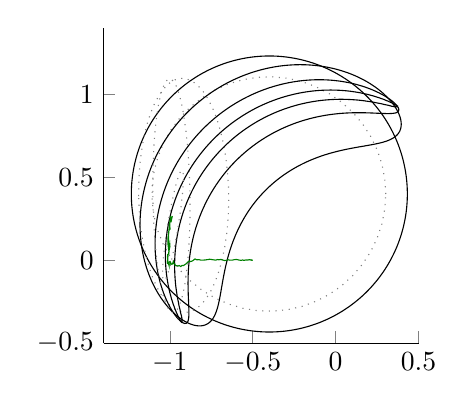
\begin{tikzpicture}

\begin{axis}[%
width=4cm,
height=4cm,
colormap={mymap}{[1pt] rgb(0pt)=(0,0,0); rgb(1pt)=(0,0,0)},
unbounded coords=jump,
scale only axis,
xmin=-1.4,
xmax=0.5,
ymin=-0.5,
ymax=1.4,
axis x line*=bottom,
axis y line*=left
]

\addplot[area legend,solid,draw=black,forget plot]
table[row sep=crcr]{
x y\\
-1.23 0.46490355595815 \\
-1.22960150659877 0.47 \\
-1.22869862032926 0.48 \\
-1.22767371065223 0.49 \\
-1.22652615959779 0.5 \\
-1.22525527442296 0.51 \\
-1.22386028691466 0.52 \\
-1.22234035261571 0.53 \\
-1.22069454997284 0.54 \\
-1.22 0.543925012252854 \\
-1.21892640279752 0.55 \\
-1.21703375996655 0.56 \\
-1.21501255351594 0.57 \\
-1.21286154858517 0.58 \\
-1.21057942808711 0.59 \\
-1.21 0.592406769213231 \\
-1.20817185045267 0.6 \\
-1.20563301512456 0.61 \\
-1.20295912720575 0.62 \\
-1.2001485327529 0.63 \\
-1.2 0.630505916752702 \\
-1.19720927177399 0.64 \\
-1.19413073501926 0.65 \\
-1.19091048235894 0.66 \\
-1.19 0.662717034143122 \\
-1.18755419286408 0.67 \\
-1.1840553713141 0.68 \\
-1.18040895669849 0.69 \\
-1.18 0.691082930921102 \\
-1.1766220430266 0.7 \\
-1.17268437715587 0.71 \\
-1.17 0.716574164360218 \\
-1.16859570678079 0.72 \\
-1.16435686868754 0.73 \\
-1.16 0.739906655398264 \\
-1.15995875610125 0.74 \\
-1.15540766506219 0.75 \\
-1.15069176174176 0.76 \\
-1.15 0.76142534514183 \\
-1.14581495754822 0.77 \\
-1.14076851906906 0.78 \\
-1.14 0.781481800290595 \\
-1.13555370431776 0.79 \\
-1.13016256518617 0.8 \\
-1.13 0.800294055571771 \\
-1.12459541368304 0.81 \\
-1.12 0.818003330802316 \\
-1.11884457213804 0.82 \\
-1.11290789864718 0.83 \\
-1.11 0.834766310779763 \\
-1.1067794262609 0.84 \\
-1.10045499989146 0.85 \\
-1.1 0.85070324293253 \\
-1.09392825155636 0.86 \\
-1.09 0.86585779537492 \\
-1.08719432959242 0.87 \\
-1.0802478170049 0.88 \\
-1.08 0.880349311626938 \\
-1.07307898957916 0.89 \\
-1.07 0.894191086141864 \\
-1.06568343026022 0.9 \\
-1.06 0.907472179329761 \\
-1.0580539964072 0.91 \\
-1.05018227493588 0.92 \\
-1.05 0.920227114822055 \\
-1.0420548844932 0.93 \\
-1.04 0.932474665837886 \\
-1.0336661072561 0.94 \\
-1.03 0.944267684379233 \\
-1.02500542583447 0.95 \\
-1.02 0.955632804221174 \\
-1.01606124067785 0.96 \\
-1.01 0.96659434215035 \\
-1.00682078403302 0.97 \\
-1 0.977174502586599 \\
-0.997270024404195 0.98 \\
-0.99 0.987393560386835 \\
-0.987393560386835 0.99 \\
-0.98 0.997270024404194 \\
-0.977174502586599 1 \\
-0.97 1.00682078403302 \\
-0.96659434215035 1.01 \\
-0.96 1.01606124067785 \\
-0.955632804221174 1.02 \\
-0.95 1.02500542583447 \\
-0.944267684379233 1.03 \\
-0.94 1.0336661072561 \\
-0.932474665837887 1.04 \\
-0.93 1.0420548844932 \\
-0.920227114822055 1.05 \\
-0.92 1.05018227493588 \\
-0.91 1.0580539964072 \\
-0.90747217932976 1.06 \\
-0.9 1.06568343026022 \\
-0.894191086141864 1.07 \\
-0.89 1.07307898957916 \\
-0.880349311626938 1.08 \\
-0.88 1.0802478170049 \\
-0.87 1.08719432959242 \\
-0.86585779537492 1.09 \\
-0.86 1.09392825155636 \\
-0.85070324293253 1.1 \\
-0.85 1.10045499989146 \\
-0.84 1.1067794262609 \\
-0.834766310779763 1.11 \\
-0.83 1.11290789864718 \\
-0.82 1.11884457213804 \\
-0.818003330802316 1.12 \\
-0.81 1.12459541368304 \\
-0.800294055571771 1.13 \\
-0.8 1.13016256518617 \\
-0.79 1.13555370431776 \\
-0.781481800290595 1.14 \\
-0.78 1.14076851906906 \\
-0.77 1.14581495754822 \\
-0.76142534514183 1.15 \\
-0.76 1.15069176174176 \\
-0.75 1.15540766506219 \\
-0.74 1.15995875610125 \\
-0.739906655398264 1.16 \\
-0.73 1.16435686868754 \\
-0.72 1.16859570678079 \\
-0.716574164360217 1.17 \\
-0.71 1.17268437715587 \\
-0.7 1.1766220430266 \\
-0.691082930921101 1.18 \\
-0.69 1.18040895669849 \\
-0.68 1.1840553713141 \\
-0.67 1.18755419286408 \\
-0.662717034143123 1.19 \\
-0.66 1.19091048235894 \\
-0.65 1.19413073501926 \\
-0.64 1.19720927177399 \\
-0.630505916752703 1.2 \\
-0.63 1.2001485327529 \\
-0.62 1.20295912720575 \\
-0.61 1.20563301512456 \\
-0.6 1.20817185045267 \\
-0.592406769213231 1.21 \\
-0.59 1.21057942808711 \\
-0.58 1.21286154858517 \\
-0.57 1.21501255351594 \\
-0.56 1.21703375996655 \\
-0.55 1.21892640279752 \\
-0.543925012252854 1.22 \\
-0.54 1.22069454997284 \\
-0.53 1.22234035261571 \\
-0.52 1.22386028691466 \\
-0.51 1.22525527442296 \\
-0.5 1.22652615959779 \\
-0.49 1.22767371065223 \\
-0.48 1.22869862032926 \\
-0.47 1.22960150659877 \\
-0.46490355595815 1.23 \\
-0.46 1.23038466003635 \\
-0.45 1.23104806991097 \\
-0.44 1.23159031728077 \\
-0.43 1.23201172796599 \\
-0.42 1.23231255504488 \\
-0.41 1.23249297910695 \\
-0.4 1.2325531084337 \\
-0.39 1.23249297910695 \\
-0.38 1.23231255504488 \\
-0.37 1.23201172796599 \\
-0.36 1.23159031728077 \\
-0.35 1.23104806991097 \\
-0.34 1.23038466003635 \\
-0.335096444041851 1.23 \\
-0.33 1.22960150659877 \\
-0.32 1.22869862032926 \\
-0.31 1.22767371065223 \\
-0.3 1.22652615959779 \\
-0.29 1.22525527442296 \\
-0.28 1.22386028691466 \\
-0.27 1.22234035261571 \\
-0.26 1.22069454997284 \\
-0.256074987747147 1.22 \\
-0.25 1.21892640279752 \\
-0.24 1.21703375996655 \\
-0.23 1.21501255351594 \\
-0.22 1.21286154858517 \\
-0.21 1.21057942808711 \\
-0.207593230786769 1.21 \\
-0.2 1.20817185045267 \\
-0.19 1.20563301512456 \\
-0.18 1.20295912720575 \\
-0.17 1.2001485327529 \\
-0.169494083247298 1.2 \\
-0.16 1.19720927177399 \\
-0.15 1.19413073501926 \\
-0.14 1.19091048235894 \\
-0.137282965856877 1.19 \\
-0.13 1.18755419286408 \\
-0.12 1.1840553713141 \\
-0.11 1.18040895669849 \\
-0.108917069078899 1.18 \\
-0.0999999999999999 1.1766220430266 \\
-0.0899999999999999 1.17268437715587 \\
-0.0834258356397825 1.17 \\
-0.0800000000000001 1.16859570678079 \\
-0.0700000000000001 1.16435686868754 \\
-0.0600933446017362 1.16 \\
-0.0600000000000001 1.15995875610125 \\
-0.05 1.15540766506219 \\
-0.04 1.15069176174176 \\
-0.0385746548581699 1.15 \\
-0.03 1.14581495754822 \\
-0.02 1.14076851906906 \\
-0.0185181997094054 1.14 \\
-0.01 1.13555370431776 \\
0 1.13016256518617 \\
0.000294055571771424 1.13 \\
0.01 1.12459541368304 \\
0.0180033308023158 1.12 \\
0.02 1.11884457213804 \\
0.03 1.11290789864718 \\
0.0347663107797624 1.11 \\
0.04 1.1067794262609 \\
0.05 1.10045499989146 \\
0.0507032429325301 1.1 \\
0.0600000000000001 1.09392825155636 \\
0.0658577953749194 1.09 \\
0.0700000000000001 1.08719432959242 \\
0.0800000000000001 1.0802478170049 \\
0.0803493116269377 1.08 \\
0.0899999999999999 1.07307898957916 \\
0.0941910861418636 1.07 \\
0.0999999999999999 1.06568343026022 \\
0.10747217932976 1.06 \\
0.11 1.0580539964072 \\
0.12 1.05018227493588 \\
0.120227114822055 1.05 \\
0.13 1.0420548844932 \\
0.132474665837886 1.04 \\
0.14 1.0336661072561 \\
0.144267684379233 1.03 \\
0.15 1.02500542583447 \\
0.155632804221174 1.02 \\
0.16 1.01606124067785 \\
0.16659434215035 1.01 \\
0.17 1.00682078403302 \\
0.1771745025866 1 \\
0.18 0.997270024404194 \\
0.187393560386835 0.99 \\
0.19 0.987393560386835 \\
0.197270024404195 0.98 \\
0.2 0.977174502586599 \\
0.206820784033018 0.97 \\
0.21 0.96659434215035 \\
0.216061240677853 0.96 \\
0.22 0.955632804221174 \\
0.225005425834474 0.95 \\
0.23 0.944267684379233 \\
0.233666107256098 0.94 \\
0.24 0.932474665837886 \\
0.242054884493204 0.93 \\
0.25 0.920227114822055 \\
0.250182274935881 0.92 \\
0.258053996407202 0.91 \\
0.26 0.907472179329761 \\
0.265683430260224 0.9 \\
0.27 0.894191086141863 \\
0.273078989579159 0.89 \\
0.28 0.880349311626938 \\
0.280247817004903 0.88 \\
0.287194329592418 0.87 \\
0.29 0.865857795374919 \\
0.293928251556358 0.86 \\
0.3 0.85070324293253 \\
0.300454999891464 0.85 \\
0.306779426260899 0.84 \\
0.31 0.834766310779762 \\
0.312907898647181 0.83 \\
0.318844572138043 0.82 \\
0.32 0.818003330802316 \\
0.324595413683044 0.81 \\
0.33 0.800294055571771 \\
0.330162565186173 0.8 \\
0.335553704317761 0.79 \\
0.34 0.781481800290595 \\
0.340768519069056 0.78 \\
0.345814957548218 0.77 \\
0.35 0.76142534514183 \\
0.350691761741762 0.76 \\
0.355407665062195 0.75 \\
0.359958756101252 0.74 \\
0.36 0.739906655398264 \\
0.364356868687543 0.73 \\
0.368595706780788 0.72 \\
0.37 0.716574164360218 \\
0.372684377155872 0.71 \\
0.376622043026596 0.7 \\
0.38 0.691082930921102 \\
0.380408956698492 0.69 \\
0.384055371314095 0.68 \\
0.387554192864077 0.67 \\
0.39 0.662717034143122 \\
0.390910482358941 0.66 \\
0.394130735019259 0.65 \\
0.397209271773994 0.64 \\
0.4 0.630505916752702 \\
0.400148532752897 0.63 \\
0.402959127205753 0.62 \\
0.405633015124562 0.61 \\
0.408171850452672 0.6 \\
0.41 0.592406769213231 \\
0.410579428087114 0.59 \\
0.41286154858517 0.58 \\
0.415012553515935 0.57 \\
0.417033759966547 0.56 \\
0.418926402797516 0.55 \\
0.42 0.543925012252854 \\
0.420694549972838 0.54 \\
0.422340352615714 0.53 \\
0.423860286914664 0.52 \\
0.425255274422965 0.51 \\
0.426526159597789 0.5 \\
0.427673710652226 0.49 \\
0.428698620329256 0.48 \\
0.429601506598767 0.47 \\
0.43 0.46490355595815 \\
0.430384660036347 0.46 \\
0.431048069910975 0.45 \\
0.431590317280767 0.44 \\
0.432011727965991 0.43 \\
0.432312555044877 0.42 \\
0.432492979106945 0.41 \\
0.432553108433699 0.4 \\
0.432492979106945 0.39 \\
0.432312555044877 0.38 \\
0.432011727965991 0.37 \\
0.431590317280767 0.36 \\
0.431048069910975 0.35 \\
0.430384660036347 0.34 \\
0.43 0.335096444041851 \\
0.429601506598767 0.33 \\
0.428698620329256 0.32 \\
0.427673710652226 0.31 \\
0.426526159597789 0.3 \\
0.425255274422965 0.29 \\
0.423860286914664 0.28 \\
0.422340352615714 0.27 \\
0.420694549972838 0.26 \\
0.42 0.256074987747147 \\
0.418926402797516 0.25 \\
0.417033759966547 0.24 \\
0.415012553515935 0.23 \\
0.41286154858517 0.22 \\
0.410579428087114 0.21 \\
0.41 0.207593230786769 \\
0.408171850452672 0.2 \\
0.405633015124562 0.19 \\
0.402959127205753 0.18 \\
0.400148532752897 0.17 \\
0.4 0.169494083247298 \\
0.397209271773994 0.16 \\
0.394130735019258 0.15 \\
0.390910482358941 0.14 \\
0.39 0.137282965856877 \\
0.387554192864077 0.13 \\
0.384055371314095 0.12 \\
0.380408956698492 0.11 \\
0.38 0.108917069078899 \\
0.376622043026596 0.0999999999999999 \\
0.372684377155872 0.0899999999999999 \\
0.37 0.0834258356397825 \\
0.368595706780788 0.0800000000000001 \\
0.364356868687543 0.0700000000000001 \\
0.36 0.0600933446017357 \\
0.359958756101252 0.0600000000000001 \\
0.355407665062195 0.05 \\
0.350691761741762 0.04 \\
0.35 0.0385746548581699 \\
0.345814957548218 0.03 \\
0.340768519069056 0.02 \\
0.34 0.0185181997094054 \\
0.335553704317761 0.01 \\
0.330162565186173 0 \\
0.33 -0.000294055571771139 \\
0.324595413683044 -0.01 \\
0.32 -0.0180033308023158 \\
0.318844572138043 -0.02 \\
0.312907898647181 -0.03 \\
0.31 -0.0347663107797621 \\
0.306779426260899 -0.04 \\
0.300454999891464 -0.05 \\
0.3 -0.0507032429325301 \\
0.293928251556357 -0.0600000000000001 \\
0.29 -0.0658577953749191 \\
0.287194329592418 -0.0700000000000001 \\
0.280247817004903 -0.0800000000000001 \\
0.28 -0.0803493116269377 \\
0.273078989579159 -0.0899999999999999 \\
0.27 -0.0941910861418633 \\
0.265683430260224 -0.0999999999999999 \\
0.26 -0.10747217932976 \\
0.258053996407202 -0.11 \\
0.250182274935881 -0.12 \\
0.25 -0.120227114822055 \\
0.242054884493204 -0.13 \\
0.24 -0.132474665837886 \\
0.233666107256098 -0.14 \\
0.23 -0.144267684379233 \\
0.225005425834474 -0.15 \\
0.22 -0.155632804221174 \\
0.216061240677853 -0.16 \\
0.21 -0.16659434215035 \\
0.206820784033018 -0.17 \\
0.2 -0.1771745025866 \\
0.197270024404195 -0.18 \\
0.19 -0.187393560386835 \\
0.187393560386835 -0.19 \\
0.18 -0.197270024404195 \\
0.1771745025866 -0.2 \\
0.17 -0.206820784033018 \\
0.16659434215035 -0.21 \\
0.16 -0.216061240677853 \\
0.155632804221174 -0.22 \\
0.15 -0.225005425834474 \\
0.144267684379233 -0.23 \\
0.14 -0.233666107256098 \\
0.132474665837886 -0.24 \\
0.13 -0.242054884493204 \\
0.120227114822055 -0.25 \\
0.12 -0.250182274935881 \\
0.11 -0.258053996407202 \\
0.10747217932976 -0.26 \\
0.0999999999999999 -0.265683430260224 \\
0.0941910861418633 -0.27 \\
0.0899999999999999 -0.273078989579159 \\
0.0803493116269377 -0.28 \\
0.0800000000000001 -0.280247817004903 \\
0.0700000000000001 -0.287194329592418 \\
0.0658577953749191 -0.29 \\
0.0600000000000001 -0.293928251556357 \\
0.0507032429325301 -0.3 \\
0.05 -0.300454999891464 \\
0.04 -0.306779426260899 \\
0.0347663107797621 -0.31 \\
0.03 -0.312907898647181 \\
0.02 -0.318844572138043 \\
0.0180033308023158 -0.32 \\
0.01 -0.324595413683044 \\
0.000294055571771139 -0.33 \\
0 -0.330162565186173 \\
-0.01 -0.335553704317761 \\
-0.0185181997094054 -0.34 \\
-0.02 -0.340768519069056 \\
-0.03 -0.345814957548218 \\
-0.0385746548581699 -0.35 \\
-0.04 -0.350691761741762 \\
-0.05 -0.355407665062195 \\
-0.0600000000000001 -0.359958756101252 \\
-0.0600933446017357 -0.36 \\
-0.0700000000000001 -0.364356868687543 \\
-0.0800000000000001 -0.368595706780788 \\
-0.0834258356397825 -0.37 \\
-0.0899999999999999 -0.372684377155872 \\
-0.0999999999999999 -0.376622043026596 \\
-0.108917069078899 -0.38 \\
-0.11 -0.380408956698492 \\
-0.12 -0.384055371314095 \\
-0.13 -0.387554192864077 \\
-0.137282965856877 -0.39 \\
-0.14 -0.390910482358941 \\
-0.15 -0.394130735019258 \\
-0.16 -0.397209271773994 \\
-0.169494083247298 -0.4 \\
-0.17 -0.400148532752897 \\
-0.18 -0.402959127205753 \\
-0.19 -0.405633015124562 \\
-0.2 -0.408171850452672 \\
-0.207593230786769 -0.41 \\
-0.21 -0.410579428087114 \\
-0.22 -0.41286154858517 \\
-0.23 -0.415012553515935 \\
-0.24 -0.417033759966547 \\
-0.25 -0.418926402797516 \\
-0.256074987747147 -0.42 \\
-0.26 -0.420694549972838 \\
-0.27 -0.422340352615714 \\
-0.28 -0.423860286914664 \\
-0.29 -0.425255274422965 \\
-0.3 -0.426526159597789 \\
-0.31 -0.427673710652226 \\
-0.32 -0.428698620329256 \\
-0.33 -0.429601506598767 \\
-0.335096444041851 -0.43 \\
-0.34 -0.430384660036347 \\
-0.35 -0.431048069910975 \\
-0.36 -0.431590317280767 \\
-0.37 -0.432011727965991 \\
-0.38 -0.432312555044877 \\
-0.39 -0.432492979106945 \\
-0.4 -0.432553108433699 \\
-0.41 -0.432492979106945 \\
-0.42 -0.432312555044877 \\
-0.43 -0.432011727965991 \\
-0.44 -0.431590317280767 \\
-0.45 -0.431048069910975 \\
-0.46 -0.430384660036347 \\
-0.46490355595815 -0.43 \\
-0.47 -0.429601506598767 \\
-0.48 -0.428698620329256 \\
-0.49 -0.427673710652226 \\
-0.5 -0.426526159597789 \\
-0.51 -0.425255274422965 \\
-0.52 -0.423860286914664 \\
-0.53 -0.422340352615714 \\
-0.54 -0.420694549972838 \\
-0.543925012252854 -0.42 \\
-0.55 -0.418926402797516 \\
-0.56 -0.417033759966547 \\
-0.57 -0.415012553515935 \\
-0.58 -0.41286154858517 \\
-0.59 -0.410579428087114 \\
-0.592406769213231 -0.41 \\
-0.6 -0.408171850452672 \\
-0.61 -0.405633015124562 \\
-0.62 -0.402959127205753 \\
-0.63 -0.400148532752897 \\
-0.630505916752703 -0.4 \\
-0.64 -0.397209271773994 \\
-0.65 -0.394130735019259 \\
-0.66 -0.390910482358941 \\
-0.662717034143123 -0.39 \\
-0.67 -0.387554192864077 \\
-0.68 -0.384055371314095 \\
-0.69 -0.380408956698492 \\
-0.691082930921101 -0.38 \\
-0.7 -0.376622043026596 \\
-0.71 -0.372684377155872 \\
-0.716574164360217 -0.37 \\
-0.72 -0.368595706780788 \\
-0.73 -0.364356868687543 \\
-0.739906655398264 -0.36 \\
-0.74 -0.359958756101252 \\
-0.75 -0.355407665062195 \\
-0.76 -0.350691761741762 \\
-0.76142534514183 -0.35 \\
-0.77 -0.345814957548218 \\
-0.78 -0.340768519069056 \\
-0.781481800290595 -0.34 \\
-0.79 -0.335553704317761 \\
-0.8 -0.330162565186173 \\
-0.800294055571771 -0.33 \\
-0.81 -0.324595413683044 \\
-0.818003330802316 -0.32 \\
-0.82 -0.318844572138043 \\
-0.83 -0.312907898647181 \\
-0.834766310779762 -0.31 \\
-0.84 -0.306779426260899 \\
-0.85 -0.300454999891464 \\
-0.85070324293253 -0.3 \\
-0.86 -0.293928251556358 \\
-0.865857795374919 -0.29 \\
-0.87 -0.287194329592418 \\
-0.88 -0.280247817004903 \\
-0.880349311626938 -0.28 \\
-0.89 -0.273078989579159 \\
-0.894191086141863 -0.27 \\
-0.9 -0.265683430260224 \\
-0.90747217932976 -0.26 \\
-0.91 -0.258053996407202 \\
-0.92 -0.250182274935881 \\
-0.920227114822055 -0.25 \\
-0.93 -0.242054884493204 \\
-0.932474665837887 -0.24 \\
-0.94 -0.233666107256098 \\
-0.944267684379233 -0.23 \\
-0.95 -0.225005425834474 \\
-0.955632804221174 -0.22 \\
-0.96 -0.216061240677853 \\
-0.96659434215035 -0.21 \\
-0.97 -0.206820784033018 \\
-0.977174502586599 -0.2 \\
-0.98 -0.197270024404195 \\
-0.987393560386835 -0.19 \\
-0.99 -0.187393560386835 \\
-0.997270024404195 -0.18 \\
-1 -0.1771745025866 \\
-1.00682078403302 -0.17 \\
-1.01 -0.16659434215035 \\
-1.01606124067785 -0.16 \\
-1.02 -0.155632804221174 \\
-1.02500542583447 -0.15 \\
-1.03 -0.144267684379233 \\
-1.0336661072561 -0.14 \\
-1.04 -0.132474665837886 \\
-1.0420548844932 -0.13 \\
-1.05 -0.120227114822055 \\
-1.05018227493588 -0.12 \\
-1.0580539964072 -0.11 \\
-1.06 -0.10747217932976 \\
-1.06568343026022 -0.0999999999999999 \\
-1.07 -0.0941910861418636 \\
-1.07307898957916 -0.0899999999999999 \\
-1.08 -0.0803493116269377 \\
-1.0802478170049 -0.0800000000000001 \\
-1.08719432959242 -0.0700000000000001 \\
-1.09 -0.0658577953749194 \\
-1.09392825155636 -0.0600000000000001 \\
-1.1 -0.0507032429325301 \\
-1.10045499989146 -0.05 \\
-1.1067794262609 -0.04 \\
-1.11 -0.0347663107797624 \\
-1.11290789864718 -0.03 \\
-1.11884457213804 -0.02 \\
-1.12 -0.0180033308023158 \\
-1.12459541368304 -0.01 \\
-1.13 -0.000294055571771424 \\
-1.13016256518617 0 \\
-1.13555370431776 0.01 \\
-1.14 0.0185181997094054 \\
-1.14076851906906 0.02 \\
-1.14581495754822 0.03 \\
-1.15 0.0385746548581699 \\
-1.15069176174176 0.04 \\
-1.15540766506219 0.05 \\
-1.15995875610125 0.0600000000000001 \\
-1.16 0.0600933446017362 \\
-1.16435686868754 0.0700000000000001 \\
-1.16859570678079 0.0800000000000001 \\
-1.17 0.0834258356397825 \\
-1.17268437715587 0.0899999999999999 \\
-1.1766220430266 0.0999999999999999 \\
-1.18 0.108917069078899 \\
-1.18040895669849 0.11 \\
-1.1840553713141 0.12 \\
-1.18755419286408 0.13 \\
-1.19 0.137282965856877 \\
-1.19091048235894 0.14 \\
-1.19413073501926 0.15 \\
-1.19720927177399 0.16 \\
-1.2 0.169494083247298 \\
-1.2001485327529 0.17 \\
-1.20295912720575 0.18 \\
-1.20563301512456 0.19 \\
-1.20817185045267 0.2 \\
-1.21 0.207593230786769 \\
-1.21057942808711 0.21 \\
-1.21286154858517 0.22 \\
-1.21501255351594 0.23 \\
-1.21703375996655 0.24 \\
-1.21892640279752 0.25 \\
-1.22 0.256074987747147 \\
-1.22069454997284 0.26 \\
-1.22234035261571 0.27 \\
-1.22386028691466 0.28 \\
-1.22525527442296 0.29 \\
-1.22652615959779 0.3 \\
-1.22767371065223 0.31 \\
-1.22869862032926 0.32 \\
-1.22960150659877 0.33 \\
-1.23 0.335096444041851 \\
-1.23038466003635 0.34 \\
-1.23104806991097 0.35 \\
-1.23159031728077 0.36 \\
-1.23201172796599 0.37 \\
-1.23231255504488 0.38 \\
-1.23249297910694 0.39 \\
-1.2325531084337 0.4 \\
-1.23249297910694 0.41 \\
-1.23231255504488 0.42 \\
-1.23201172796599 0.43 \\
-1.23159031728077 0.44 \\
-1.23104806991097 0.45 \\
-1.23038466003635 0.46 \\
-1.23 0.46490355595815 \\
NaN NaN \\
};

\addplot [
color=gray,
dotted,
forget plot
]
table[row sep=crcr]{
0.302360541231733 0.4\\
0.2965696634757 0.490422808186003\\
0.279292116260257 0.579360876361465\\
0.250811596433019 0.665353843905771\\
0.211595753342162 0.746989708669247\\
0.162288510047058 0.822928012009422\\
0.10369949011944 0.891921849084879\\
0.0367907236467382 0.952838342998275\\
-0.0373391492753579 1.00467724660368\\
-0.117472918182899 1.04658736653706\\
-0.202294788805839 1.07788053978777\\
-0.290411988373579 1.09804293331619\\
-0.380377634905347 1.10674348117799\\
-0.470714494972326 1.10383932061783\\
-0.559939239829713 1.08937813787181\\
-0.646586801633701 1.06359738516082\\
-0.729234429814971 1.02692038173164\\
-0.806525052603702 0.979949362966567\\
-0.877189560110518 0.923455591695151\\
-0.940067643075783 0.858366694079811\\
-0.994126845115566 0.785751428019912\\
-1.03847951562692 0.7068021341766\\
-1.07239738498625 0.622815157772112\\
-1.09532352271638 0.535169562637062\\
-1.1068814822696 0.445304487020476\\
-1.1068814822696 0.354695512979524\\
-1.09532352271638 0.264830437362938\\
-1.07239738498625 0.177184842227889\\
-1.03847951562692 0.0931978658233998\\
-0.994126845115566 0.0142485719800879\\
-0.940067643075784 -0.058366694079811\\
-0.877189560110518 -0.123455591695151\\
-0.806525052603702 -0.179949362966567\\
-0.729234429814971 -0.226920381731638\\
-0.646586801633701 -0.263597385160825\\
-0.559939239829713 -0.28937813787181\\
-0.470714494972325 -0.303839320617828\\
-0.380377634905347 -0.30674348117799\\
-0.29041198837358 -0.298042933316187\\
-0.20229478880584 -0.277880539787771\\
-0.117472918182899 -0.246587366537059\\
-0.0373391492753583 -0.204677246603681\\
0.036790723646738 -0.152838342998275\\
0.103699490119439 -0.0919218490848791\\
0.162288510047058 -0.0229280120094228\\
0.211595753342162 0.0530102913307532\\
0.250811596433019 0.134646156094229\\
0.279292116260257 0.220639123638535\\
0.2965696634757 0.309577191813997\\
0.302360541231733 0.4\\
};

\addplot[area legend,solid,draw=black,forget plot]
table[row sep=crcr]{
x y\\
-1.17 0.34824483234669 \\
-1.16974685063192 0.35 \\
-1.16819226362119 0.36 \\
-1.16652579083749 0.37 \\
-1.16474640465062 0.38 \\
-1.16285290186727 0.39 \\
-1.16084389340103 0.4 \\
-1.16 0.403972283004096 \\
-1.15872752024962 0.41 \\
-1.15650161857746 0.42 \\
-1.15415850992452 0.43 \\
-1.15169620345948 0.44 \\
-1.15 0.446570497508841 \\
-1.14911957270876 0.45 \\
-1.14643582378503 0.46 \\
-1.14362995065294 0.47 \\
-1.14069920346947 0.48 \\
-1.14 0.482292669864651 \\
-1.13766087050511 0.49 \\
-1.13450203673762 0.5 \\
-1.13121376409444 0.51 \\
-1.13 0.513558350248353 \\
-1.1278116203584 0.52 \\
-1.12428796612075 0.53 \\
-1.12062893201116 0.54 \\
-1.12 0.541663477723823 \\
-1.11685840800488 0.55 \\
-1.11295502020046 0.56 \\
-1.11 0.56731503463497 \\
-1.1089179667055 0.57 \\
-1.10476285025168 0.58 \\
-1.10046101620946 0.59 \\
-1.1 0.591041770839401 \\
-1.09604227319328 0.6 \\
-1.09147623443274 0.61 \\
-1.09 0.613142166756836 \\
-1.08678076273977 0.62 \\
-1.08194080954232 0.63 \\
-1.08 0.633899158806308 \\
-1.07696335112985 0.64 \\
-1.07183867003779 0.65 \\
-1.07 0.653493256137173 \\
-1.06657249843507 0.66 \\
-1.06115098587887 0.67 \\
-1.06 0.672071557680547 \\
-1.05558789116181 0.68 \\
-1.05 0.689751052742826 \\
-1.04985699636204 0.69 \\
-1.04398616547374 0.7 \\
-1.04 0.706603959589081 \\
-1.03794361838801 0.71 \\
-1.03174054970386 0.72 \\
-1.03 0.722741706044418 \\
-1.02537385112673 0.73 \\
-1.02 0.738216777058695 \\
-1.01882821800339 0.74 \\
-1.01211523648097 0.75 \\
-1.01 0.753080756290404 \\
-1.00522296955145 0.76 \\
-1 0.767388077842723 \\
-0.998141887321532 0.77 \\
-0.990874145928976 0.78 \\
-0.99 0.781179799014672 \\
-0.983418455088601 0.79 \\
-0.98 0.794483082457343 \\
-0.975760203119438 0.8 \\
-0.97 0.807340585135123 \\
-0.967895220180388 0.81 \\
-0.96 0.819777404251693 \\
-0.959818579796784 0.82 \\
-0.951530102936964 0.83 \\
-0.95 0.831812067722366 \\
-0.943015865809287 0.84 \\
-0.94 0.843472184497663 \\
-0.934268290314526 0.85 \\
-0.93 0.854777416654995 \\
-0.925279730157293 0.86 \\
-0.92 0.865745241610559 \\
-0.916041674018024 0.87 \\
-0.91 0.876391723329543 \\
-0.906544708951422 0.88 \\
-0.9 0.886731619659182 \\
-0.896778476336056 0.89 \\
-0.89 0.896778476336056 \\
-0.886731619659182 0.9 \\
-0.88 0.906544708951422 \\
-0.876391723329543 0.91 \\
-0.87 0.916041674018024 \\
-0.865745241610559 0.92 \\
-0.86 0.925279730157293 \\
-0.854777416654995 0.93 \\
-0.85 0.934268290314526 \\
-0.843472184497663 0.94 \\
-0.84 0.943015865809288 \\
-0.831812067722366 0.95 \\
-0.83 0.951530102936965 \\
-0.82 0.959818579796784 \\
-0.819777404251693 0.96 \\
-0.81 0.967895220180388 \\
-0.807340585135122 0.97 \\
-0.8 0.975760203119437 \\
-0.794483082457343 0.98 \\
-0.79 0.983418455088602 \\
-0.781179799014672 0.99 \\
-0.78 0.990874145928976 \\
-0.77 0.998141887321532 \\
-0.767388077842723 1 \\
-0.76 1.00522296955145 \\
-0.753080756290404 1.01 \\
-0.75 1.01211523648097 \\
-0.74 1.01882821800339 \\
-0.738216777058696 1.02 \\
-0.73 1.02537385112673 \\
-0.722741706044418 1.03 \\
-0.72 1.03174054970386 \\
-0.71 1.03794361838801 \\
-0.706603959589081 1.04 \\
-0.7 1.04398616547375 \\
-0.69 1.04985699636204 \\
-0.689751052742826 1.05 \\
-0.68 1.05558789116181 \\
-0.672071557680547 1.06 \\
-0.67 1.06115098587887 \\
-0.66 1.06657249843507 \\
-0.653493256137172 1.07 \\
-0.65 1.07183867003779 \\
-0.64 1.07696335112985 \\
-0.633899158806308 1.08 \\
-0.63 1.08194080954232 \\
-0.62 1.08678076273977 \\
-0.613142166756836 1.09 \\
-0.61 1.09147623443274 \\
-0.6 1.09604227319328 \\
-0.591041770839401 1.1 \\
-0.59 1.10046101620946 \\
-0.58 1.10476285025168 \\
-0.57 1.1089179667055 \\
-0.56731503463497 1.11 \\
-0.56 1.11295502020045 \\
-0.55 1.11685840800488 \\
-0.541663477723823 1.12 \\
-0.54 1.12062893201116 \\
-0.53 1.12428796612075 \\
-0.52 1.1278116203584 \\
-0.513558350248353 1.13 \\
-0.51 1.13121376409444 \\
-0.5 1.13450203673762 \\
-0.49 1.13766087050511 \\
-0.482292669864651 1.14 \\
-0.48 1.14069920346947 \\
-0.47 1.14362995065294 \\
-0.46 1.14643582378503 \\
-0.45 1.14911957270876 \\
-0.446570497508841 1.15 \\
-0.44 1.15169620345948 \\
-0.43 1.15415850992452 \\
-0.42 1.15650161857746 \\
-0.41 1.15872752024962 \\
-0.403972283004096 1.16 \\
-0.4 1.16084389340103 \\
-0.39 1.16285290186727 \\
-0.38 1.16474640465062 \\
-0.37 1.16652579083749 \\
-0.36 1.16819226362119 \\
-0.35 1.16974685063192 \\
-0.34824483234669 1.17 \\
-0.34 1.17119736332875 \\
-0.33 1.17253708306572 \\
-0.32 1.17376516554583 \\
-0.31 1.17488223536639 \\
-0.3 1.17588878364361 \\
-0.29 1.17678517647896 \\
-0.28 1.17757166314514 \\
-0.27 1.17824838400104 \\
-0.26 1.17881537814023 \\
-0.25 1.17927259077445 \\
-0.24 1.17961988034923 \\
-0.23 1.1798570253855 \\
-0.22 1.17998373103776 \\
-0.21 1.17999963535578 \\
-0.2 1.17990431523439 \\
-0.19 1.17969729203277 \\
-0.18 1.17937803684251 \\
-0.17 1.17894597538143 \\
-0.16 1.17840049248854 \\
-0.15 1.17774093619399 \\
-0.14 1.1769666213368 \\
-0.13 1.17607683270263 \\
-0.12 1.17507082765349 \\
-0.11 1.17394783822133 \\
-0.0999999999999999 1.17270707263833 \\
-0.0899999999999999 1.17134771627709 \\
-0.0808808221553111 1.17 \\
-0.0800000000000001 1.169868446055 \\
-0.0700000000000001 1.16826318492631 \\
-0.0600000000000001 1.1665358522753 \\
-0.05 1.16468558953898 \\
-0.04 1.16271152558355 \\
-0.03 1.16061277372685 \\
-0.0272297162274458 1.16 \\
-0.02 1.15837707043464 \\
-0.01 1.15600950424899 \\
0 1.15351353518583 \\
0.01 1.15088831903331 \\
0.0132417961451759 1.15 \\
0.02 1.1481144843506 \\
0.03 1.1451998014171 \\
0.04 1.14215236860539 \\
0.0467845809778874 1.14 \\
0.05 1.13895839590464 \\
0.0600000000000001 1.13560172760492 \\
0.0700000000000001 1.13210924568362 \\
0.0758326192762357 1.13 \\
0.0800000000000001 1.12845705211644 \\
0.0899999999999999 1.12463447377779 \\
0.0999999999999999 1.12067372352401 \\
0.101654875861228 1.12 \\
0.11 1.11651329321956 \\
0.12 1.11220142977958 \\
0.124965625555616 1.11 \\
0.13 1.10770379085866 \\
0.14 1.10302068977659 \\
0.146281627658991 1.1 \\
0.15 1.09815606221167 \\
0.16 1.09308122969512 \\
0.165927999060679 1.09 \\
0.17 1.08781244454026 \\
0.18 1.08232554760214 \\
0.18415237085094 1.08 \\
0.19 1.07660791404929 \\
0.2 1.07068940384791 \\
0.201145721652617 1.07 \\
0.21 1.06447069599288 \\
0.217032177449418 1.06 \\
0.22 1.05803665457619 \\
0.23 1.05132313374821 \\
0.231943882101265 1.05 \\
0.24 1.04428372571177 \\
0.245958520328016 1.04 \\
0.25 1.03696310983243 \\
0.259164215758356 1.03 \\
0.26 1.02933444169534 \\
0.27 1.02130039326315 \\
0.27160451321306 1.02 \\
0.28 1.01285817275248 \\
0.283336244087455 1.01 \\
0.29 1.0039916294524 \\
0.29440365869371 1 \\
0.3 0.994646303613179 \\
0.30483949801983 0.99 \\
0.31 0.984756110397065 \\
0.314671396184423 0.98 \\
0.32 0.974240900702571 \\
0.323922474439262 0.97 \\
0.33 0.963003381220004 \\
0.332611869145027 0.96 \\
0.34 0.950925197880764 \\
0.340755206485876 0.95 \\
0.348353919103909 0.94 \\
0.35 0.937660090845779 \\
0.355419004395882 0.93 \\
0.36 0.922984220900905 \\
0.361962087595305 0.92 \\
0.36797165252887 0.91 \\
0.37 0.906270424491979 \\
0.373443745141697 0.9 \\
0.378378429548447 0.89 \\
0.38 0.8862599122459 \\
0.382748545988888 0.88 \\
0.386543456781287 0.87 \\
0.389749012796172 0.86 \\
0.39 0.859001026024989 \\
0.392300698766757 0.85 \\
0.394180890645867 0.84 \\
0.395336251754202 0.83 \\
0.395697015250948 0.82 \\
0.395176614410703 0.81 \\
0.39366754926419 0.8 \\
0.391035889986567 0.79 \\
0.39 0.787258661419913 \\
0.38705697916176 0.78 \\
0.381513307702241 0.77 \\
0.38 0.76784594377993 \\
0.374007445086244 0.76 \\
0.37 0.7557514351253 \\
0.364054295499889 0.75 \\
0.36 0.746700822030463 \\
0.350894547332186 0.74 \\
0.35 0.739430738915723 \\
0.34 0.733546956944958 \\
0.333298499271874 0.73 \\
0.33 0.728449374871357 \\
0.32 0.724105387704512 \\
0.31 0.720189628818945 \\
0.30948537538196 0.72 \\
0.3 0.716820146879085 \\
0.29 0.713742733243921 \\
0.28 0.710905686344939 \\
0.276631981808553 0.71 \\
0.27 0.708348249786546 \\
0.26 0.705990225868927 \\
0.25 0.703765986162755 \\
0.24 0.701653387666864 \\
0.231856513506836 0.7 \\
0.23 0.699645189000129 \\
0.22 0.697762633450779 \\
0.21 0.695933040344062 \\
0.2 0.694143056983395 \\
0.19 0.692380555671002 \\
0.18 0.690634479159236 \\
0.176397789260313 0.69 \\
0.17 0.688922459583778 \\
0.16 0.687221648864136 \\
0.15 0.685507533384693 \\
0.14 0.683772550733038 \\
0.13 0.682009658682955 \\
0.12 0.680212272727076 \\
0.118859861177737 0.68 \\
0.11 0.678404402725216 \\
0.0999999999999999 0.676553533757192 \\
0.0899999999999999 0.674650364964621 \\
0.0800000000000001 0.672689883309064 \\
0.0700000000000001 0.670667299751165 \\
0.0668306100783585 0.67 \\
0.0600000000000001 0.668597853651372 \\
0.05 0.66646691237605 \\
0.04 0.664260949803104 \\
0.03 0.661976004677973 \\
0.0216673934388655 0.66 \\
0.02 0.659612293922447 \\
0.01 0.657183320094115 \\
0 0.65466475610035 \\
-0.01 0.652053104374175 \\
-0.017567454667616 0.65 \\
-0.02 0.649349850941758 \\
-0.03 0.646563140809441 \\
-0.04 0.643674188237087 \\
-0.05 0.640679674329226 \\
-0.052180207372021 0.64 \\
-0.0600000000000001 0.637589219183333 \\
-0.0700000000000001 0.63439166581964 \\
-0.0800000000000001 0.631080205491351 \\
-0.0831402257352855 0.63 \\
-0.0899999999999999 0.627659442913738 \\
-0.0999999999999999 0.624123550351529 \\
-0.11 0.620465748641229 \\
-0.111227012060718 0.62 \\
-0.12 0.616688410403288 \\
-0.13 0.612785488763925 \\
-0.136900064685736 0.61 \\
-0.14 0.60875277155352 \\
-0.15 0.604588741202766 \\
-0.16 0.600290571267089 \\
-0.16065351031315 0.6 \\
-0.17 0.595850011960966 \\
-0.18 0.591270707191558 \\
-0.182687213649655 0.59 \\
-0.19 0.586540695511637 \\
-0.2 0.581664556411378 \\
-0.203310270220351 0.58 \\
-0.21 0.576629475148341 \\
-0.22 0.571440830887073 \\
-0.222695730199283 0.57 \\
-0.23 0.566082636343688 \\
-0.24 0.56056576211472 \\
-0.240996536634055 0.56 \\
-0.25 0.554864283969042 \\
-0.25829823208705 0.55 \\
-0.26 0.548996397299665 \\
-0.27 0.542936451594461 \\
-0.274718974924906 0.54 \\
-0.28 0.53669018665601 \\
-0.29 0.530259090650918 \\
-0.290392682652562 0.53 \\
-0.3 0.523608996367508 \\
-0.305292522306472 0.52 \\
-0.31 0.516760031015857 \\
-0.31958736311537 0.51 \\
-0.32 0.509706038368183 \\
-0.33 0.502411592496721 \\
-0.333230504355639 0.5 \\
-0.34 0.494889881614602 \\
-0.346333666426978 0.49 \\
-0.35 0.487135070921797 \\
-0.358933405813462 0.48 \\
-0.36 0.479137028373567 \\
-0.37 0.470872491657892 \\
-0.371034071904004 0.47 \\
-0.38 0.462330832836047 \\
-0.382670783399685 0.46 \\
-0.39 0.45351036479971 \\
-0.393888241389502 0.45 \\
-0.4 0.444397399512695 \\
-0.404707850571412 0.44 \\
-0.41 0.434977128695799 \\
-0.415149914587216 0.43 \\
-0.42 0.425233637932722 \\
-0.425233637932722 0.42 \\
-0.43 0.415149914587216 \\
-0.434977128695799 0.41 \\
-0.44 0.404707850571412 \\
-0.444397399512695 0.4 \\
-0.45 0.393888241389502 \\
-0.45351036479971 0.39 \\
-0.46 0.382670783399685 \\
-0.462330832836047 0.38 \\
-0.47 0.371034071904004 \\
-0.470872491657892 0.37 \\
-0.479137028373567 0.36 \\
-0.48 0.358933405813462 \\
-0.487135070921797 0.35 \\
-0.49 0.346333666426978 \\
-0.494889881614602 0.34 \\
-0.5 0.333230504355639 \\
-0.502411592496721 0.33 \\
-0.509706038368183 0.32 \\
-0.51 0.31958736311537 \\
-0.516760031015857 0.31 \\
-0.52 0.305292522306472 \\
-0.523608996367508 0.3 \\
-0.53 0.290392682652562 \\
-0.530259090650918 0.29 \\
-0.53669018665601 0.28 \\
-0.54 0.274718974924906 \\
-0.542936451594461 0.27 \\
-0.548996397299665 0.26 \\
-0.55 0.25829823208705 \\
-0.554864283969042 0.25 \\
-0.56 0.240996536634055 \\
-0.560565762114719 0.24 \\
-0.566082636343688 0.23 \\
-0.57 0.222695730199283 \\
-0.571440830887073 0.22 \\
-0.576629475148341 0.21 \\
-0.58 0.203310270220351 \\
-0.581664556411378 0.2 \\
-0.586540695511637 0.19 \\
-0.59 0.182687213649655 \\
-0.591270707191558 0.18 \\
-0.595850011960966 0.17 \\
-0.6 0.16065351031315 \\
-0.600290571267089 0.16 \\
-0.604588741202766 0.15 \\
-0.60875277155352 0.14 \\
-0.61 0.136900064685736 \\
-0.612785488763925 0.13 \\
-0.616688410403289 0.12 \\
-0.62 0.111227012060718 \\
-0.620465748641228 0.11 \\
-0.624123550351529 0.0999999999999999 \\
-0.627659442913738 0.0899999999999999 \\
-0.63 0.0831402257352855 \\
-0.631080205491351 0.0800000000000001 \\
-0.63439166581964 0.0700000000000001 \\
-0.637589219183333 0.0600000000000001 \\
-0.64 0.052180207372021 \\
-0.640679674329226 0.05 \\
-0.643674188237087 0.04 \\
-0.64656314080944 0.03 \\
-0.649349850941758 0.02 \\
-0.65 0.017567454667616 \\
-0.652053104374176 0.01 \\
-0.654664756100351 0 \\
-0.657183320094115 -0.01 \\
-0.659612293922446 -0.02 \\
-0.66 -0.0216673934388655 \\
-0.661976004677973 -0.03 \\
-0.664260949803104 -0.04 \\
-0.66646691237605 -0.05 \\
-0.668597853651372 -0.0600000000000001 \\
-0.67 -0.0668306100783585 \\
-0.670667299751165 -0.0700000000000001 \\
-0.672689883309064 -0.0800000000000001 \\
-0.674650364964621 -0.0899999999999999 \\
-0.676553533757192 -0.0999999999999999 \\
-0.678404402725216 -0.11 \\
-0.68 -0.118859861177737 \\
-0.680212272727076 -0.12 \\
-0.682009658682955 -0.13 \\
-0.683772550733038 -0.14 \\
-0.685507533384693 -0.15 \\
-0.687221648864136 -0.16 \\
-0.688922459583777 -0.17 \\
-0.69 -0.176397789260313 \\
-0.690634479159236 -0.18 \\
-0.692380555671002 -0.19 \\
-0.694143056983395 -0.2 \\
-0.695933040344063 -0.21 \\
-0.697762633450779 -0.22 \\
-0.699645189000129 -0.23 \\
-0.7 -0.231856513506836 \\
-0.701653387666865 -0.24 \\
-0.703765986162755 -0.25 \\
-0.705990225868927 -0.26 \\
-0.708348249786546 -0.27 \\
-0.71 -0.276631981808553 \\
-0.71090568634494 -0.28 \\
-0.713742733243921 -0.29 \\
-0.716820146879085 -0.3 \\
-0.72 -0.30948537538196 \\
-0.720189628818945 -0.31 \\
-0.724105387704512 -0.32 \\
-0.728449374871357 -0.33 \\
-0.73 -0.333298499271874 \\
-0.733546956944958 -0.34 \\
-0.739430738915724 -0.35 \\
-0.74 -0.350894547332186 \\
-0.746700822030463 -0.36 \\
-0.75 -0.364054295499889 \\
-0.7557514351253 -0.37 \\
-0.76 -0.374007445086244 \\
-0.767845943779929 -0.38 \\
-0.77 -0.381513307702241 \\
-0.78 -0.38705697916176 \\
-0.787258661419913 -0.39 \\
-0.79 -0.391035889986567 \\
-0.8 -0.39366754926419 \\
-0.81 -0.395176614410703 \\
-0.82 -0.395697015250948 \\
-0.83 -0.395336251754202 \\
-0.84 -0.394180890645867 \\
-0.85 -0.392300698766757 \\
-0.859001026024989 -0.39 \\
-0.86 -0.389749012796172 \\
-0.87 -0.386543456781287 \\
-0.88 -0.382748545988888 \\
-0.8862599122459 -0.38 \\
-0.89 -0.378378429548447 \\
-0.9 -0.373443745141697 \\
-0.906270424491979 -0.37 \\
-0.91 -0.36797165252887 \\
-0.92 -0.361962087595305 \\
-0.922984220900905 -0.36 \\
-0.93 -0.355419004395882 \\
-0.93766009084578 -0.35 \\
-0.94 -0.348353919103909 \\
-0.95 -0.340755206485876 \\
-0.950925197880764 -0.34 \\
-0.96 -0.332611869145027 \\
-0.963003381220003 -0.33 \\
-0.97 -0.323922474439262 \\
-0.974240900702571 -0.32 \\
-0.98 -0.314671396184423 \\
-0.984756110397065 -0.31 \\
-0.99 -0.30483949801983 \\
-0.994646303613179 -0.3 \\
-1 -0.29440365869371 \\
-1.0039916294524 -0.29 \\
-1.01 -0.283336244087455 \\
-1.01285817275248 -0.28 \\
-1.02 -0.27160451321306 \\
-1.02130039326315 -0.27 \\
-1.02933444169534 -0.26 \\
-1.03 -0.259164215758356 \\
-1.03696310983243 -0.25 \\
-1.04 -0.245958520328016 \\
-1.04428372571177 -0.24 \\
-1.05 -0.231943882101265 \\
-1.05132313374821 -0.23 \\
-1.05803665457619 -0.22 \\
-1.06 -0.217032177449418 \\
-1.06447069599288 -0.21 \\
-1.07 -0.201145721652617 \\
-1.07068940384791 -0.2 \\
-1.07660791404929 -0.19 \\
-1.08 -0.18415237085094 \\
-1.08232554760214 -0.18 \\
-1.08781244454026 -0.17 \\
-1.09 -0.165927999060679 \\
-1.09308122969512 -0.16 \\
-1.09815606221167 -0.15 \\
-1.1 -0.146281627658991 \\
-1.10302068977659 -0.14 \\
-1.10770379085866 -0.13 \\
-1.11 -0.124965625555616 \\
-1.11220142977958 -0.12 \\
-1.11651329321956 -0.11 \\
-1.12 -0.101654875861228 \\
-1.12067372352401 -0.0999999999999999 \\
-1.12463447377779 -0.0899999999999999 \\
-1.12845705211644 -0.0800000000000001 \\
-1.13 -0.0758326192762357 \\
-1.13210924568362 -0.0700000000000001 \\
-1.13560172760492 -0.0600000000000001 \\
-1.13895839590464 -0.05 \\
-1.14 -0.0467845809778874 \\
-1.14215236860539 -0.04 \\
-1.1451998014171 -0.03 \\
-1.1481144843506 -0.02 \\
-1.15 -0.0132417961451759 \\
-1.15088831903331 -0.01 \\
-1.15351353518583 0 \\
-1.15600950424899 0.01 \\
-1.15837707043464 0.02 \\
-1.16 0.0272297162274458 \\
-1.16061277372685 0.03 \\
-1.16271152558355 0.04 \\
-1.16468558953898 0.05 \\
-1.1665358522753 0.0600000000000001 \\
-1.16826318492631 0.0700000000000001 \\
-1.169868446055 0.0800000000000001 \\
-1.17 0.0808808221553111 \\
-1.17134771627709 0.0899999999999999 \\
-1.17270707263833 0.0999999999999999 \\
-1.17394783822133 0.11 \\
-1.17507082765349 0.12 \\
-1.17607683270263 0.13 \\
-1.1769666213368 0.14 \\
-1.17774093619399 0.15 \\
-1.17840049248854 0.16 \\
-1.17894597538143 0.17 \\
-1.17937803684251 0.18 \\
-1.17969729203277 0.19 \\
-1.17990431523439 0.2 \\
-1.17999963535578 0.21 \\
-1.17998373103776 0.22 \\
-1.1798570253855 0.23 \\
-1.17961988034923 0.24 \\
-1.17927259077445 0.25 \\
-1.17881537814023 0.26 \\
-1.17824838400104 0.27 \\
-1.17757166314514 0.28 \\
-1.17678517647896 0.29 \\
-1.17588878364361 0.3 \\
-1.17488223536639 0.31 \\
-1.17376516554583 0.32 \\
-1.17253708306572 0.33 \\
-1.17119736332875 0.34 \\
-1.17 0.34824483234669 \\
NaN NaN \\
};

\addplot [
color=gray,
dotted,
forget plot
]
table[row sep=crcr]{
-1.18816259276298 0.387660825716958\\
-1.1872623009542 0.478024200150298\\
-1.18191806302077 0.566969413672885\\
-1.17221763120181 0.653035988337699\\
-1.15832028631961 0.734810713368186\\
-1.14045422239291 0.810950850040126\\
-1.11891279969747 0.880206179414376\\
-1.09404972779839 0.941439530897277\\
-1.06627325764888 0.993645454550367\\
-1.03603947812088 1.03596673055057\\
-1.00384482703837 1.06770844471601\\
-0.970217939682064 1.08834939897762\\
-0.935710968612685 1.09755066943708\\
-0.900890517341195 1.09516117148784\\
-0.86632833671481 1.08122014062015\\
-0.83259193678389 1.05595648817544\\
-0.800235268302609 1.01978504262841\\
-0.769789626872881 0.97329973811492\\
-0.741754929085267 0.917263862049928\\
-0.716591503902378 0.852597521969227\\
-0.694712534070037 0.780362537389144\\
-0.676477271668014 0.701745004759439\\
-0.662185139200809 0.618035821792394\\
-0.652070813088407 0.530609490958062\\
-0.646300370285948 0.440901550191711\\
-0.644968561304716 0.350385001400616\\
-0.648097254411361 0.26054612381346\\
-0.655635076551572 0.172860069316495\\
-0.667458256894199 0.0887666405003501\\
-0.683372659144886 0.00964664914129715\\
-0.703116969258655 -0.0632007566899383\\
-0.726366986209299 -0.128579424603582\\
-0.752740945361268 -0.185415838679984\\
-0.781805787034435 -0.232776746571336\\
-0.813084267332069 -0.269884483479426\\
-0.846062794472421 -0.296129741390121\\
-0.880199861951588 -0.311081573894117\\
-0.914934940065332 -0.314494472315065\\
-0.949697679791329 -0.306312396955246\\
-0.983917277904345 -0.286669697265864\\
-1.01703184954942 -0.255888905832766\\
-1.04849765437563 -0.214475442400303\\
-1.07779802473767 -0.163109314893099\\
-1.10445184936423 -0.102633953704729\\
-1.12802147319183 -0.0340423625939751\\
-1.14811988364885 0.0415391864094429\\
-1.16441706539122 0.122869646360451\\
-1.17664541914529 0.208613573355158\\
-1.18460415568051 0.297363054482828\\
-1.18816259276298 0.387660825716957\\
};

\addplot[area legend,solid,draw=black,forget plot]
table[row sep=crcr]{
x y\\
-1.08 0.231100501158994 \\
-1.07871196895865 0.24 \\
-1.07715886677485 0.25 \\
-1.07549877520187 0.26 \\
-1.073729226905 0.27 \\
-1.07184711715049 0.28 \\
-1.07 0.28924301708876 \\
-1.0698500519161 0.29 \\
-1.06775793738537 0.3 \\
-1.06555568832225 0.31 \\
-1.06323842644563 0.32 \\
-1.06080035677995 0.33 \\
-1.06 0.333127338095644 \\
-1.05826036304034 0.34 \\
-1.05561488001036 0.35 \\
-1.05284770266877 0.36 \\
-1.05 0.369828745506068 \\
-1.04995085831684 0.37 \\
-1.04696825367183 0.38 \\
-1.04386103713728 0.39 \\
-1.04061806973452 0.4 \\
-1.04 0.40183437771208 \\
-1.03727957536703 0.41 \\
-1.03381936150804 0.42 \\
-1.0302140006715 0.43 \\
-1.03 0.430573570296294 \\
-1.02652185472898 0.44 \\
-1.02269099497391 0.45 \\
-1.02 0.456764849853095 \\
-1.01872477090524 0.46 \\
-1.01465772283711 0.47 \\
-1.01043012432748 0.48 \\
-1.01 0.480986835601705 \\
-1.0061091515928 0.49 \\
-1.001633452438 0.5 \\
-1 0.503534272941972 \\
-0.997036250928217 0.51 \\
-0.992300523762823 0.52 \\
-0.99 0.524702421819395 \\
-0.987426657057749 0.53 \\
-0.98241805132332 0.54 \\
-0.98 0.544677085422287 \\
-0.97726492395677 0.55 \\
-0.971968814856949 0.56 \\
-0.97 0.563609163138297 \\
-0.966532331088546 0.57 \\
-0.96093124959039 0.58 \\
-0.96 0.581620338708095 \\
-0.95520622028468 0.59 \\
-0.95 0.598802014012256 \\
-0.949293091822093 0.6 \\
-0.943258836531548 0.61 \\
-0.94 0.615238610570856 \\
-0.937043596862247 0.62 \\
-0.930655644188156 0.63 \\
-0.93 0.631003486606561 \\
-0.924129990682321 0.64 \\
-0.92 0.646145788544833 \\
-0.917408840785191 0.65 \\
-0.910507261450283 0.66 \\
-0.91 0.660719880676243 \\
-0.903454781809262 0.67 \\
-0.9 0.674768258275351 \\
-0.896199953338119 0.68 \\
-0.89 0.688321971589354 \\
-0.888744907651233 0.69 \\
-0.881108320144735 0.7 \\
-0.88 0.701421472456822 \\
-0.873281237105897 0.71 \\
-0.87 0.714093916723676 \\
-0.865238705316014 0.72 \\
-0.86 0.726358323860261 \\
-0.85697830205961 0.73 \\
-0.85 0.738239009950063 \\
-0.848496131171515 0.74 \\
-0.84 0.749757599509426 \\
-0.839786954404004 0.75 \\
-0.830856571326686 0.76 \\
-0.83 0.760942459170614 \\
-0.821682771900772 0.77 \\
-0.82 0.771801653639525 \\
-0.812254601273068 0.78 \\
-0.81 0.78234886994885 \\
-0.802563202953863 0.79 \\
-0.8 0.792598441865324 \\
-0.792598441865324 0.8 \\
-0.79 0.802563202953863 \\
-0.782348869948849 0.81 \\
-0.78 0.812254601273068 \\
-0.771801653639525 0.82 \\
-0.77 0.821682771900772 \\
-0.760942459170614 0.83 \\
-0.76 0.830856571326686 \\
-0.75 0.839786954404004 \\
-0.749757599509426 0.84 \\
-0.74 0.848496131171515 \\
-0.738239009950063 0.85 \\
-0.73 0.85697830205961 \\
-0.726358323860261 0.86 \\
-0.72 0.865238705316014 \\
-0.714093916723676 0.87 \\
-0.71 0.873281237105897 \\
-0.701421472456823 0.88 \\
-0.7 0.881108320144735 \\
-0.69 0.888744907651233 \\
-0.688321971589354 0.89 \\
-0.68 0.896199953338119 \\
-0.674768258275351 0.9 \\
-0.67 0.903454781809262 \\
-0.660719880676243 0.91 \\
-0.66 0.910507261450283 \\
-0.65 0.917408840785191 \\
-0.646145788544833 0.92 \\
-0.64 0.924129990682321 \\
-0.631003486606561 0.93 \\
-0.63 0.930655644188156 \\
-0.62 0.937043596862247 \\
-0.615238610570855 0.94 \\
-0.61 0.943258836531547 \\
-0.6 0.949293091822093 \\
-0.598802014012256 0.95 \\
-0.59 0.95520622028468 \\
-0.581620338708095 0.96 \\
-0.58 0.96093124959039 \\
-0.57 0.966532331088546 \\
-0.563609163138297 0.97 \\
-0.56 0.971968814856949 \\
-0.55 0.97726492395677 \\
-0.544677085422287 0.98 \\
-0.54 0.98241805132332 \\
-0.53 0.987426657057749 \\
-0.524702421819395 0.99 \\
-0.52 0.992300523762823 \\
-0.51 0.997036250928216 \\
-0.503534272941972 1 \\
-0.5 1.001633452438 \\
-0.49 1.0061091515928 \\
-0.480986835601705 1.01 \\
-0.48 1.01043012432748 \\
-0.47 1.01465772283711 \\
-0.46 1.01872477090524 \\
-0.456764849853095 1.02 \\
-0.45 1.02269099497391 \\
-0.44 1.02652185472898 \\
-0.430573570296294 1.03 \\
-0.43 1.0302140006715 \\
-0.42 1.03381936150804 \\
-0.41 1.03727957536703 \\
-0.40183437771208 1.04 \\
-0.4 1.04061806973452 \\
-0.39 1.04386103713728 \\
-0.38 1.04696825367183 \\
-0.37 1.04995085831684 \\
-0.369828745506068 1.05 \\
-0.36 1.05284770266877 \\
-0.35 1.05561488001036 \\
-0.34 1.05826036304034 \\
-0.333127338095644 1.06 \\
-0.33 1.06080035677995 \\
-0.32 1.06323842644563 \\
-0.31 1.06555568832225 \\
-0.3 1.06775793738537 \\
-0.29 1.0698500519161 \\
-0.28924301708876 1.07 \\
-0.28 1.07184711715049 \\
-0.27 1.073729226905 \\
-0.26 1.07549877520187 \\
-0.25 1.07715886677485 \\
-0.24 1.07871196895865 \\
-0.231100501158994 1.08 \\
-0.23 1.08016060373913 \\
-0.22 1.08150600395464 \\
-0.21 1.08274140002999 \\
-0.2 1.0838683675727 \\
-0.19 1.08488807679557 \\
-0.18 1.08580134003942 \\
-0.17 1.08660865732347 \\
-0.16 1.08731026014377 \\
-0.15 1.08790615363971 \\
-0.14 1.0883961571525 \\
-0.13 1.08877994310866 \\
-0.12 1.08905707407818 \\
-0.11 1.08922703778153 \\
-0.0999999999999999 1.08928927975559 \\
-0.0899999999999999 1.08924323333672 \\
-0.0800000000000001 1.08908834658221 \\
-0.0700000000000001 1.0888241057304 \\
-0.0600000000000001 1.08845005479673 \\
-0.05 1.08796581091743 \\
-0.04 1.08737107508538 \\
-0.03 1.08666563797215 \\
-0.02 1.0858493805946 \\
-0.01 1.08492226966087 \\
0 1.08388434751616 \\
0.01 1.08273571669792 \\
0.02 1.08147651920039 \\
0.03 1.08010691063288 \\
0.0307276857574095 1.08 \\
0.04 1.07858201174444 \\
0.05 1.07694206720129 \\
0.0600000000000001 1.07519166749251 \\
0.0700000000000001 1.07333177564159 \\
0.0800000000000001 1.07136323983982 \\
0.0865798632628309 1.07 \\
0.0899999999999999 1.06925371115579 \\
0.0999999999999999 1.06697375704064 \\
0.11 1.0645904732933 \\
0.12 1.0621052628966 \\
0.128147354696822 1.06 \\
0.13 1.05949084294268 \\
0.14 1.05665526618276 \\
0.15 1.05372969264873 \\
0.16 1.05071522309294 \\
0.162308432284779 1.05 \\
0.17 1.04744832709888 \\
0.18 1.04405911555294 \\
0.19 1.04059969135822 \\
0.191697087992291 1.04 \\
0.2 1.03683425906385 \\
0.21 1.0329749083527 \\
0.217610406051705 1.03 \\
0.22 1.02898092520807 \\
0.23 1.02467775359008 \\
0.24 1.02036608407703 \\
0.240839207448693 1.02 \\
0.25 1.01562074388462 \\
0.26 1.01087471524753 \\
0.261833168653785 1.01 \\
0.27 1.00568962344203 \\
0.28 1.00049471410504 \\
0.280950766622242 1 \\
0.29 0.994746114652752 \\
0.298380617432425 0.99 \\
0.3 0.988957506470421 \\
0.31 0.982634292740129 \\
0.314270521655032 0.98 \\
0.32 0.975947213593388 \\
0.328752899792541 0.97 \\
0.33 0.969005047721411 \\
0.34 0.961327538476326 \\
0.341794399231137 0.96 \\
0.35 0.952810034420689 \\
0.353386004400784 0.95 \\
0.36 0.943286458036441 \\
0.363452163928866 0.94 \\
0.37 0.93202582122935 \\
0.371792406831813 0.93 \\
0.377953320715041 0.92 \\
0.38 0.913375479082374 \\
0.38116593234548 0.91 \\
0.38 0.902548887073039 \\
0.379435646911342 0.9 \\
0.37 0.892322576254617 \\
0.36510053780348 0.89 \\
0.36 0.888659096767959 \\
0.35 0.886921098375069 \\
0.34 0.885893362977098 \\
0.33 0.885343314814909 \\
0.32 0.885122344125088 \\
0.31 0.885131182994241 \\
0.3 0.88530105429508 \\
0.29 0.885582807823807 \\
0.28 0.885940360347682 \\
0.27 0.886346577232306 \\
0.26 0.886780600486731 \\
0.25 0.887226065991875 \\
0.24 0.887669885125762 \\
0.23 0.888101394776476 \\
0.22 0.888511753781863 \\
0.21 0.888893507826222 \\
0.2 0.889240271724396 \\
0.19 0.889546494900803 \\
0.18 0.889807286705906 \\
0.170885568293288 0.89 \\
0.17 0.890019630849657 \\
0.16 0.890187726005517 \\
0.15 0.890293550066543 \\
0.14 0.890334394317231 \\
0.13 0.890307733181963 \\
0.12 0.890211188794005 \\
0.11 0.890042502604192 \\
0.108275559465236 0.89 \\
0.0999999999999999 0.889809182899413 \\
0.0899999999999999 0.889504209749728 \\
0.0800000000000001 0.889123271762044 \\
0.0700000000000001 0.888664315277602 \\
0.0600000000000001 0.888125387410358 \\
0.05 0.887504619689706 \\
0.04 0.886800210345281 \\
0.03 0.886010404615147 \\
0.02 0.885133472505886 \\
0.01 0.88416768345981 \\
0 0.883111277391459 \\
-0.01 0.881962431542163 \\
-0.02 0.880719222565898 \\
-0.0253522944409747 0.88 \\
-0.03 0.879393264588734 \\
-0.04 0.877987935274297 \\
-0.05 0.876486204148372 \\
-0.0600000000000001 0.874886401785733 \\
-0.0700000000000001 0.873186618966573 \\
-0.0800000000000001 0.871384638790016 \\
-0.0872530695413777 0.87 \\
-0.0899999999999999 0.86948437345958 \\
-0.0999999999999999 0.867498963315115 \\
-0.11 0.865411160823111 \\
-0.12 0.863218501042108 \\
-0.13 0.860917921556042 \\
-0.133798061171009 0.86 \\
-0.14 0.858516209042918 \\
-0.15 0.856015165259509 \\
-0.16 0.853407042116975 \\
-0.17 0.850687631719005 \\
-0.172420262539036 0.85 \\
-0.18 0.84785823331026 \\
-0.19 0.844923567609797 \\
-0.2 0.841878384937672 \\
-0.205934056782075 0.84 \\
-0.21 0.838714281027752 \\
-0.22 0.835437728888576 \\
-0.23 0.832051110102252 \\
-0.235845730669139 0.83 \\
-0.24 0.828539695933917 \\
-0.25 0.824909418094436 \\
-0.26 0.821168010184014 \\
-0.263018246933328 0.82 \\
-0.27 0.817288961770428 \\
-0.28 0.813295087619737 \\
-0.288013137093527 0.81 \\
-0.29 0.809177609617848 \\
-0.3 0.804918029901843 \\
-0.31 0.800549512237306 \\
-0.311220165317026 0.8 \\
-0.32 0.796021120138474 \\
-0.33 0.791382546874732 \\
-0.332898048443387 0.79 \\
-0.34 0.786584877170496 \\
-0.35 0.781667486986992 \\
-0.353302858842512 0.78 \\
-0.36 0.776587951808929 \\
-0.37 0.771384583418183 \\
-0.37259415206925 0.77 \\
-0.38 0.766008383183035 \\
-0.39 0.760512666192364 \\
-0.390909546448445 0.76 \\
-0.4 0.754824203858405 \\
-0.408316847351266 0.75 \\
-0.41 0.749011331744172 \\
-0.42 0.743013354254727 \\
-0.424924876443613 0.74 \\
-0.43 0.73685647638296 \\
-0.44 0.730552851034899 \\
-0.440857575042382 0.73 \\
-0.45 0.724036610740097 \\
-0.456082864031417 0.72 \\
-0.46 0.717365836503548 \\
-0.47 0.710527934954821 \\
-0.470756112251481 0.71 \\
-0.48 0.703464692731714 \\
-0.484820023955895 0.7 \\
-0.49 0.696225752921387 \\
-0.498410865232533 0.69 \\
-0.5 0.688806651589942 \\
-0.51 0.681170647170178 \\
-0.51150579528578 0.68 \\
-0.52 0.673307153216941 \\
-0.52413148231521 0.67 \\
-0.53 0.66523616170411 \\
-0.536351937809481 0.66 \\
-0.54 0.656949059162205 \\
-0.548184706202455 0.65 \\
-0.55 0.648435911497382 \\
-0.559645977656083 0.64 \\
-0.56 0.639685742041906 \\
-0.57 0.630668638878126 \\
-0.570730034122072 0.63 \\
-0.58 0.621387890888826 \\
-0.581471649085517 0.62 \\
-0.59 0.61184011718157 \\
-0.591894847606257 0.61 \\
-0.6 0.602013297919568 \\
-0.602013297919568 0.6 \\
-0.61 0.591894847606257 \\
-0.61184011718157 0.59 \\
-0.62 0.581471649085517 \\
-0.621387890888826 0.58 \\
-0.63 0.570730034122072 \\
-0.630668638878126 0.57 \\
-0.639685742041906 0.56 \\
-0.64 0.559645977656083 \\
-0.648435911497383 0.55 \\
-0.65 0.548184706202455 \\
-0.656949059162205 0.54 \\
-0.66 0.536351937809481 \\
-0.66523616170411 0.53 \\
-0.67 0.52413148231521 \\
-0.673307153216941 0.52 \\
-0.68 0.51150579528578 \\
-0.681170647170178 0.51 \\
-0.688806651589942 0.5 \\
-0.69 0.498410865232533 \\
-0.696225752921387 0.49 \\
-0.7 0.484820023955895 \\
-0.703464692731714 0.48 \\
-0.71 0.470756112251481 \\
-0.710527934954821 0.47 \\
-0.717365836503548 0.46 \\
-0.72 0.456082864031417 \\
-0.724036610740097 0.45 \\
-0.73 0.440857575042382 \\
-0.7305528510349 0.44 \\
-0.73685647638296 0.43 \\
-0.74 0.424924876443613 \\
-0.743013354254727 0.42 \\
-0.749011331744172 0.41 \\
-0.75 0.408316847351266 \\
-0.754824203858405 0.4 \\
-0.76 0.390909546448445 \\
-0.760512666192364 0.39 \\
-0.766008383183035 0.38 \\
-0.77 0.37259415206925 \\
-0.771384583418183 0.37 \\
-0.776587951808929 0.36 \\
-0.78 0.353302858842512 \\
-0.781667486986992 0.35 \\
-0.786584877170496 0.34 \\
-0.79 0.332898048443387 \\
-0.791382546874732 0.33 \\
-0.796021120138474 0.32 \\
-0.8 0.311220165317026 \\
-0.800549512237306 0.31 \\
-0.804918029901843 0.3 \\
-0.809177609617848 0.29 \\
-0.81 0.288013137093527 \\
-0.813295087619736 0.28 \\
-0.817288961770428 0.27 \\
-0.82 0.263018246933328 \\
-0.821168010184014 0.26 \\
-0.824909418094436 0.25 \\
-0.828539695933916 0.24 \\
-0.83 0.235845730669139 \\
-0.832051110102253 0.23 \\
-0.835437728888577 0.22 \\
-0.838714281027752 0.21 \\
-0.84 0.205934056782075 \\
-0.841878384937673 0.2 \\
-0.844923567609797 0.19 \\
-0.84785823331026 0.18 \\
-0.85 0.172420262539036 \\
-0.850687631719005 0.17 \\
-0.853407042116975 0.16 \\
-0.85601516525951 0.15 \\
-0.858516209042918 0.14 \\
-0.86 0.133798061171009 \\
-0.860917921556042 0.13 \\
-0.863218501042108 0.12 \\
-0.865411160823111 0.11 \\
-0.867498963315115 0.0999999999999999 \\
-0.86948437345958 0.0899999999999999 \\
-0.87 0.0872530695413777 \\
-0.871384638790016 0.0800000000000001 \\
-0.873186618966573 0.0700000000000001 \\
-0.874886401785734 0.0600000000000001 \\
-0.876486204148371 0.05 \\
-0.877987935274297 0.04 \\
-0.879393264588734 0.03 \\
-0.88 0.0253522944409747 \\
-0.880719222565898 0.02 \\
-0.881962431542163 0.01 \\
-0.883111277391459 0 \\
-0.88416768345981 -0.01 \\
-0.885133472505886 -0.02 \\
-0.886010404615147 -0.03 \\
-0.886800210345281 -0.04 \\
-0.887504619689706 -0.05 \\
-0.888125387410358 -0.0600000000000001 \\
-0.888664315277602 -0.0700000000000001 \\
-0.889123271762044 -0.0800000000000001 \\
-0.889504209749728 -0.0899999999999999 \\
-0.889809182899413 -0.0999999999999999 \\
-0.89 -0.108275559465236 \\
-0.890042502604192 -0.11 \\
-0.890211188794006 -0.12 \\
-0.890307733181963 -0.13 \\
-0.89033439431723 -0.14 \\
-0.890293550066543 -0.15 \\
-0.890187726005517 -0.16 \\
-0.890019630849657 -0.17 \\
-0.89 -0.170885568293288 \\
-0.889807286705906 -0.18 \\
-0.889546494900803 -0.19 \\
-0.889240271724396 -0.2 \\
-0.888893507826222 -0.21 \\
-0.888511753781863 -0.22 \\
-0.888101394776476 -0.23 \\
-0.887669885125762 -0.24 \\
-0.887226065991875 -0.25 \\
-0.886780600486731 -0.26 \\
-0.886346577232306 -0.27 \\
-0.885940360347682 -0.28 \\
-0.885582807823807 -0.29 \\
-0.88530105429508 -0.3 \\
-0.885131182994241 -0.31 \\
-0.885122344125088 -0.32 \\
-0.885343314814909 -0.33 \\
-0.885893362977098 -0.34 \\
-0.88692109837507 -0.35 \\
-0.888659096767959 -0.36 \\
-0.89 -0.36510053780348 \\
-0.892322576254617 -0.37 \\
-0.9 -0.379435646911342 \\
-0.902548887073039 -0.38 \\
-0.91 -0.38116593234548 \\
-0.913375479082374 -0.38 \\
-0.92 -0.377953320715041 \\
-0.93 -0.371792406831813 \\
-0.93202582122935 -0.37 \\
-0.94 -0.363452163928866 \\
-0.943286458036441 -0.36 \\
-0.95 -0.353386004400784 \\
-0.952810034420689 -0.35 \\
-0.96 -0.341794399231137 \\
-0.961327538476325 -0.34 \\
-0.969005047721411 -0.33 \\
-0.97 -0.328752899792541 \\
-0.975947213593389 -0.32 \\
-0.98 -0.314270521655032 \\
-0.982634292740129 -0.31 \\
-0.98895750647042 -0.3 \\
-0.99 -0.298380617432425 \\
-0.994746114652752 -0.29 \\
-1 -0.280950766622242 \\
-1.00049471410504 -0.28 \\
-1.00568962344203 -0.27 \\
-1.01 -0.261833168653785 \\
-1.01087471524753 -0.26 \\
-1.01562074388462 -0.25 \\
-1.02 -0.240839207448693 \\
-1.02036608407703 -0.24 \\
-1.02467775359008 -0.23 \\
-1.02898092520807 -0.22 \\
-1.03 -0.217610406051705 \\
-1.0329749083527 -0.21 \\
-1.03683425906385 -0.2 \\
-1.04 -0.191697087992291 \\
-1.04059969135822 -0.19 \\
-1.04405911555294 -0.18 \\
-1.04744832709888 -0.17 \\
-1.05 -0.162308432284779 \\
-1.05071522309294 -0.16 \\
-1.05372969264873 -0.15 \\
-1.05665526618276 -0.14 \\
-1.05949084294268 -0.13 \\
-1.06 -0.128147354696822 \\
-1.0621052628966 -0.12 \\
-1.0645904732933 -0.11 \\
-1.06697375704064 -0.0999999999999999 \\
-1.06925371115579 -0.0899999999999999 \\
-1.07 -0.0865798632628309 \\
-1.07136323983982 -0.0800000000000001 \\
-1.07333177564159 -0.0700000000000001 \\
-1.07519166749251 -0.0600000000000001 \\
-1.07694206720129 -0.05 \\
-1.07858201174444 -0.04 \\
-1.08 -0.0307276857574095 \\
-1.08010691063288 -0.03 \\
-1.08147651920039 -0.02 \\
-1.08273571669792 -0.01 \\
-1.08388434751616 0 \\
-1.08492226966087 0.01 \\
-1.0858493805946 0.02 \\
-1.08666563797215 0.03 \\
-1.08737107508538 0.04 \\
-1.08796581091743 0.05 \\
-1.08845005479673 0.0600000000000001 \\
-1.0888241057304 0.0700000000000001 \\
-1.08908834658221 0.0800000000000001 \\
-1.08924323333672 0.0899999999999999 \\
-1.08928927975559 0.0999999999999999 \\
-1.08922703778153 0.11 \\
-1.08905707407818 0.12 \\
-1.08877994310866 0.13 \\
-1.0883961571525 0.14 \\
-1.08790615363971 0.15 \\
-1.08731026014377 0.16 \\
-1.08660865732347 0.17 \\
-1.08580134003942 0.18 \\
-1.08488807679557 0.19 \\
-1.0838683675727 0.2 \\
-1.08274140002999 0.21 \\
-1.08150600395464 0.22 \\
-1.08016060373913 0.23 \\
-1.08 0.231100501158994 \\
NaN NaN \\
};

\addplot [
color=gray,
dotted,
forget plot
]
table[row sep=crcr]{
-1.10263132211871 0.387339239181597\\
-1.10039271121502 0.297205288174882\\
-1.09635267268689 0.208578240297176\\
-1.09057754385526 0.122913349224404\\
-1.08316215217589 0.0416172300996476\\
-1.07422825817514 -0.0339752370486181\\
-1.06392255614551 -0.102622825999685\\
-1.05241426542941 -0.163198345240841\\
-1.03989235184223 -0.214707146420847\\
-1.0265624248589 -0.256303456448366\\
-1.01264336151195 -0.287304265062737\\
-0.998363712436719 -0.307200539843576\\
-0.983957949076248 -0.315665584509044\\
-0.969662613666646 -0.312560403259763\\
-0.955712435220121 -0.297935983085998\\
-0.942336475281092 -0.27203245656269\\
-0.92975436674196 -0.235275158879208\\
-0.918172707477086 -0.188267643847305\\
-0.907781668011406 -0.131781773564213\\
-0.898751868925673 -0.066745044458344\\
-0.89123157927123 0.00577464217642237\\
-0.885344281996294 0.0845865150904571\\
-0.881186646359358 0.168396485509383\\
-0.878826940622634 0.255828396035975\\
-0.878303911089083 0.345446617116571\\
-0.879626145889185 0.435779620038657\\
-0.882771933964079 0.525344139391642\\
-0.887689621560544 0.612669528243897\\
-0.894298460384202 0.696321906124707\\
-0.902489933484282 0.774927703301964\\
-0.912129537098945 0.847196214759192\\
-0.923058989203339 0.911940793536235\\
-0.935098828496072 0.968098335439534\\
-0.948051361148816 1.0147467351836\\
-0.961703906933504 1.05112002733429\\
-0.975832291425799 1.07662096344009\\
-0.990204526942935 1.09083081883515\\
-1.00458462177506 1.09351626808675\\
-1.0187364551626 1.0846332161924\\
-1.03242765439257 1.06432752261864\\
-1.04543341035214 1.03293260629256\\
-1.057540168888 0.990963970872276\\
-1.06854913735971 0.939110740191102\\
-1.07827954880932 0.878224342863266\\
-1.08657163014985 0.809304531849594\\
-1.09328922563492 0.73348296854154\\
-1.09832203253239 0.652004640912422\\
-1.10158741229215 0.56620742084932\\
-1.10303174746881 0.477500096333679\\
-1.10263132211871 0.387339239181597\\
};

\addplot[area legend,solid,draw=black,forget plot]
table[row sep=crcr]{
x y\\
-1.02 0.14755918924672 \\
-1.01970062957614 0.15 \\
-1.01838307731108 0.16 \\
-1.01699047863097 0.17 \\
-1.01551283194511 0.18 \\
-1.01393622513793 0.19 \\
-1.01224226451811 0.2 \\
-1.01040727082665 0.21 \\
-1.01 0.21205692199292 \\
-1.00845331727653 0.22 \\
-1.00644108232613 0.23 \\
-1.00433846484406 0.24 \\
-1.00210618335128 0.25 \\
-1 0.258763518177516 \\
-0.999704836524284 0.26 \\
-0.99724703527667 0.27 \\
-0.994713189740226 0.28 \\
-0.992038407393629 0.29 \\
-0.99 0.29710927231001 \\
-0.989185921275777 0.3 \\
-0.986308081791391 0.31 \\
-0.983320204361811 0.32 \\
-0.980122791116227 0.33 \\
-0.98 0.330363934721412 \\
-0.976889631963748 0.34 \\
-0.973560789959073 0.35 \\
-0.97 0.359998160806209 \\
-0.969999353820787 0.36 \\
-0.966431807154835 0.37 \\
-0.96273154952828 0.38 \\
-0.96 0.386915334435363 \\
-0.958812318359577 0.39 \\
-0.954898486009438 0.4 \\
-0.9507551771809 0.41 \\
-0.95 0.41173041182146 \\
-0.946543794107179 0.42 \\
-0.942206044902763 0.43 \\
-0.94 0.434788450046519 \\
-0.937676620644901 0.44 \\
-0.933106203875306 0.45 \\
-0.93 0.456385097597214 \\
-0.928288016837838 0.46 \\
-0.923459219973677 0.47 \\
-0.92 0.4767328398229 \\
-0.918362331709927 0.48 \\
-0.913253590057176 0.49 \\
-0.91 0.495996405815997 \\
-0.907882770668161 0.5 \\
-0.90246488635776 0.51 \\
-0.9 0.514303235373764 \\
-0.896830170150973 0.52 \\
-0.891051379844843 0.53 \\
-0.89 0.53173997717109 \\
-0.88517467917021 0.54 \\
-0.88 0.548397737615277 \\
-0.879026196597864 0.55 \\
-0.87286048216777 0.56 \\
-0.87 0.564399814477977 \\
-0.866439255468405 0.57 \\
-0.86 0.579694496174818 \\
-0.859798495466364 0.58 \\
-0.853143839934967 0.59 \\
-0.85 0.594489392961915 \\
-0.84620664110753 0.6 \\
-0.84 0.608660877754899 \\
-0.83904607424349 0.61 \\
-0.831807343462472 0.62 \\
-0.83 0.622396405655752 \\
-0.82435405378511 0.63 \\
-0.82 0.635634725916127 \\
-0.816651917268189 0.64 \\
-0.81 0.648396648980263 \\
-0.808730750256785 0.65 \\
-0.800646641526317 0.66 \\
-0.8 0.660777752324408 \\
-0.79239445172812 0.67 \\
-0.79 0.672807834138415 \\
-0.783884126466318 0.68 \\
-0.78 0.684438684428004 \\
-0.775126147326692 0.69 \\
-0.77 0.695706609793648 \\
-0.766123709808474 0.7 \\
-0.76 0.706638740912526 \\
-0.756874639324438 0.71 \\
-0.75 0.717255949138561 \\
-0.747372929012496 0.72 \\
-0.74 0.727574980935669 \\
-0.73760990478892 0.73 \\
-0.73 0.73760990478892 \\
-0.727574980935669 0.74 \\
-0.72 0.747372929012496 \\
-0.717255949138561 0.75 \\
-0.71 0.756874639324438 \\
-0.706638740912525 0.76 \\
-0.7 0.766123709808474 \\
-0.695706609793648 0.77 \\
-0.69 0.775126147326692 \\
-0.684438684428004 0.78 \\
-0.68 0.783884126466318 \\
-0.672807834138415 0.79 \\
-0.67 0.792394451728119 \\
-0.660777752324408 0.8 \\
-0.66 0.800646641526317 \\
-0.65 0.808730750256785 \\
-0.648396648980263 0.81 \\
-0.64 0.816651917268189 \\
-0.635634725916128 0.82 \\
-0.63 0.82435405378511 \\
-0.622396405655752 0.83 \\
-0.62 0.831807343462472 \\
-0.61 0.83904607424349 \\
-0.608660877754899 0.84 \\
-0.6 0.84620664110753 \\
-0.594489392961915 0.85 \\
-0.59 0.853143839934967 \\
-0.58 0.859798495466364 \\
-0.579694496174818 0.86 \\
-0.57 0.866439255468405 \\
-0.564399814477977 0.87 \\
-0.56 0.87286048216777 \\
-0.55 0.879026196597864 \\
-0.548397737615277 0.88 \\
-0.54 0.88517467917021 \\
-0.53173997717109 0.89 \\
-0.53 0.891051379844843 \\
-0.52 0.896830170150973 \\
-0.514303235373764 0.9 \\
-0.51 0.90246488635776 \\
-0.5 0.907882770668161 \\
-0.495996405815997 0.91 \\
-0.49 0.913253590057176 \\
-0.48 0.918362331709927 \\
-0.4767328398229 0.92 \\
-0.47 0.923459219973677 \\
-0.46 0.928288016837838 \\
-0.456385097597214 0.93 \\
-0.45 0.933106203875306 \\
-0.44 0.937676620644901 \\
-0.434788450046519 0.94 \\
-0.43 0.942206044902763 \\
-0.42 0.946543794107179 \\
-0.41173041182146 0.95 \\
-0.41 0.9507551771809 \\
-0.4 0.954898486009439 \\
-0.39 0.958812318359577 \\
-0.386915334435363 0.96 \\
-0.38 0.962731549528281 \\
-0.37 0.966431807154835 \\
-0.36 0.969999353820787 \\
-0.359998160806209 0.97 \\
-0.35 0.973560789959073 \\
-0.34 0.976889631963748 \\
-0.330363934721412 0.98 \\
-0.33 0.980122791116227 \\
-0.32 0.983320204361811 \\
-0.31 0.986308081791391 \\
-0.3 0.989185921275777 \\
-0.29710927231001 0.99 \\
-0.29 0.992038407393629 \\
-0.28 0.994713189740225 \\
-0.27 0.99724703527667 \\
-0.26 0.999704836524284 \\
-0.258763518177516 1 \\
-0.25 1.00210618335128 \\
-0.24 1.00433846484406 \\
-0.23 1.00644108232613 \\
-0.22 1.00845331727653 \\
-0.21205692199292 1.01 \\
-0.21 1.01040727082665 \\
-0.2 1.01224226451811 \\
-0.19 1.01393622513793 \\
-0.18 1.01551283194511 \\
-0.17 1.01699047863097 \\
-0.16 1.01838307731108 \\
-0.15 1.01970062957614 \\
-0.14755918924672 1.02 \\
-0.14 1.02091022128828 \\
-0.13 1.02199091010107 \\
-0.12 1.02295672235703 \\
-0.11 1.02381444122063 \\
-0.0999999999999999 1.02456859813662 \\
-0.0899999999999999 1.02522189634409 \\
-0.0800000000000001 1.02577559344503 \\
-0.0700000000000001 1.02622985652358 \\
-0.0600000000000001 1.02658409669628 \\
-0.05 1.02683728383785 \\
-0.04 1.02698823676751 \\
-0.03 1.02703587980079 \\
-0.02 1.02697945376788 \\
-0.01 1.02681866881486 \\
0 1.02655378775537 \\
0.01 1.02618563229086 \\
0.02 1.02571550951746 \\
0.03 1.02514506189258 \\
0.04 1.024476049169 \\
0.05 1.02371007470122 \\
0.0600000000000001 1.02284827024592 \\
0.0700000000000001 1.02189095259276 \\
0.0800000000000001 1.02083726218628 \\
0.0872738092153846 1.02 \\
0.0899999999999999 1.01962716389809 \\
0.0999999999999999 1.01818452237758 \\
0.11 1.0166879387898 \\
0.12 1.01513763634716 \\
0.13 1.01353017956582 \\
0.14 1.01185838487782 \\
0.15 1.01011118761908 \\
0.150602719262658 1.01 \\
0.16 1.00788580575705 \\
0.17 1.00568619211232 \\
0.18 1.00351136695204 \\
0.19 1.0013279317073 \\
0.195911555732821 1 \\
0.2 0.998805423254191 \\
0.21 0.99599049040874 \\
0.22 0.993333162964336 \\
0.23 0.990746403933393 \\
0.232809144923679 0.99 \\
0.24 0.987461343274258 \\
0.25 0.984254647914138 \\
0.26 0.981287994994543 \\
0.26433413761277 0.98 \\
0.27 0.977632917880478 \\
0.28 0.973950849220506 \\
0.29 0.970687109988611 \\
0.292082553797754 0.97 \\
0.3 0.966224171054656 \\
0.31 0.962352153524284 \\
0.316673024878377 0.96 \\
0.32 0.958046997642995 \\
0.33 0.953301742292812 \\
0.338758760107018 0.95 \\
0.34 0.949048485251704 \\
0.35 0.943234762900698 \\
0.358000678597395 0.94 \\
0.36 0.937731188241127 \\
0.37 0.931547685272737 \\
0.373549569783289 0.93 \\
0.37 0.92590417238061 \\
0.36 0.926014774372348 \\
0.35 0.927433628727718 \\
0.34 0.929087395546929 \\
0.335296344556496 0.93 \\
0.33 0.931751945171512 \\
0.32 0.934459803750481 \\
0.31 0.936633988423144 \\
0.3 0.938597468864151 \\
0.292766312010264 0.94 \\
0.29 0.940798534083597 \\
0.28 0.943420572101871 \\
0.27 0.945565886223837 \\
0.26 0.947465132036725 \\
0.25 0.949226829571654 \\
0.245584309370475 0.95 \\
0.24 0.951298135799519 \\
0.23 0.953349740486469 \\
0.22 0.955119947566257 \\
0.21 0.956707858921035 \\
0.2 0.958169510265262 \\
0.19 0.959538258338327 \\
0.186526651891418 0.96 \\
0.18 0.961076529040474 \\
0.17 0.962537409120815 \\
0.16 0.963814881966997 \\
0.15 0.964948871461857 \\
0.14 0.965964365436626 \\
0.13 0.966877072544146 \\
0.12 0.967696659843189 \\
0.11 0.968428723791199 \\
0.0999999999999999 0.969076060995182 \\
0.0899999999999999 0.969639533306527 \\
0.08250435758392 0.97 \\
0.0800000000000001 0.970139786524216 \\
0.0700000000000001 0.970591971566713 \\
0.0600000000000001 0.970930869363449 \\
0.05 0.971162086053415 \\
0.04 0.971289193775423 \\
0.03 0.971314262868526 \\
0.02 0.971238203999555 \\
0.01 0.971060968830129 \\
0 0.970781636139031 \\
-0.01 0.970398396020533 \\
-0.0181242403698377 0.97 \\
-0.02 0.96991645904084 \\
-0.03 0.969371932254177 \\
-0.04 0.968731524055555 \\
-0.05 0.967995483938644 \\
-0.0600000000000001 0.96716362293418 \\
-0.0700000000000001 0.966234955865743 \\
-0.0800000000000001 0.965207253967614 \\
-0.0899999999999999 0.964076479820496 \\
-0.0999999999999999 0.962836059068974 \\
-0.11 0.961475915189021 \\
-0.119874969285356 0.96 \\
-0.12 0.959981782831166 \\
-0.13 0.958427445291411 \\
-0.14 0.956791110746096 \\
-0.15 0.955063444825229 \\
-0.16 0.953229209025145 \\
-0.17 0.951265224294165 \\
-0.175979152106759 0.95 \\
-0.18 0.949156577579589 \\
-0.19 0.946981870821992 \\
-0.2 0.944732151802402 \\
-0.21 0.942374183310072 \\
-0.219448489345274 0.94 \\
-0.22 0.939859162484961 \\
-0.23 0.937225887365629 \\
-0.24 0.934541532159736 \\
-0.25 0.931750594075865 \\
-0.255917373852917 0.93 \\
-0.26 0.928773467235168 \\
-0.27 0.925719739471731 \\
-0.28 0.92260110458949 \\
-0.287943147714988 0.92 \\
-0.29 0.919306574578067 \\
-0.3 0.915884393282043 \\
-0.31 0.912420446012407 \\
-0.316679460430597 0.91 \\
-0.32 0.908760324762218 \\
-0.33 0.904996999935072 \\
-0.34 0.901177369735418 \\
-0.342938235701457 0.9 \\
-0.35 0.897113276869397 \\
-0.36 0.89302875128681 \\
-0.367181858528521 0.89 \\
-0.37 0.888766029061808 \\
-0.38 0.88437232951325 \\
-0.389828606577766 0.88 \\
-0.39 0.879919995188851 \\
-0.4 0.875202863263915 \\
-0.41 0.87049678427856 \\
-0.411010902969959 0.87 \\
-0.42 0.865500059690607 \\
-0.43 0.860521676698212 \\
-0.431005517743451 0.86 \\
-0.44 0.855242071090322 \\
-0.449968728202597 0.85 \\
-0.45 0.849982724143182 \\
-0.46 0.844411394452151 \\
-0.467926595284003 0.84 \\
-0.47 0.83879598526351 \\
-0.48 0.832993344191345 \\
-0.4850821953647 0.83 \\
-0.49 0.827005573429674 \\
-0.5 0.820966413425064 \\
-0.501550781924906 0.82 \\
-0.51 0.814616711653142 \\
-0.51725834212013 0.81 \\
-0.52 0.808189108774379 \\
-0.53 0.801610629975585 \\
-0.532393390381072 0.8 \\
-0.54 0.794757922503879 \\
-0.546909104773811 0.79 \\
-0.55 0.787797530539543 \\
-0.56 0.780707285642437 \\
-0.560971655827691 0.78 \\
-0.57 0.773300804862504 \\
-0.574423876911498 0.77 \\
-0.58 0.765730051356495 \\
-0.587481995718896 0.76 \\
-0.59 0.758012095261676 \\
-0.6 0.750136093573186 \\
-0.600168488585009 0.75 \\
-0.61 0.74192829157792 \\
-0.612324537921668 0.74 \\
-0.62 0.733510036948803 \\
-0.62411666471005 0.73 \\
-0.63 0.724879760995039 \\
-0.635564337519429 0.72 \\
-0.64 0.716028628634581 \\
-0.646680181424324 0.71 \\
-0.65 0.70694335899622 \\
-0.657473493891969 0.7 \\
-0.66 0.697608474921384 \\
-0.667952743241237 0.69 \\
-0.67 0.688008089280374 \\
-0.678127240749404 0.68 \\
-0.68 0.678127240749404 \\
-0.688008089280373 0.67 \\
-0.69 0.667952743241237 \\
-0.697608474921384 0.66 \\
-0.7 0.657473493891969 \\
-0.706943358996221 0.65 \\
-0.71 0.646680181424323 \\
-0.716028628634581 0.64 \\
-0.72 0.635564337519429 \\
-0.724879760995039 0.63 \\
-0.73 0.62411666471005 \\
-0.733510036948803 0.62 \\
-0.74 0.612324537921668 \\
-0.74192829157792 0.61 \\
-0.75 0.600168488585009 \\
-0.750136093573185 0.6 \\
-0.758012095261676 0.59 \\
-0.76 0.587481995718895 \\
-0.765730051356494 0.58 \\
-0.77 0.574423876911498 \\
-0.773300804862505 0.57 \\
-0.78 0.560971655827691 \\
-0.780707285642437 0.56 \\
-0.787797530539543 0.55 \\
-0.79 0.546909104773811 \\
-0.794757922503879 0.54 \\
-0.8 0.532393390381072 \\
-0.801610629975585 0.53 \\
-0.808189108774379 0.52 \\
-0.81 0.51725834212013 \\
-0.814616711653142 0.51 \\
-0.82 0.501550781924906 \\
-0.820966413425064 0.5 \\
-0.827005573429674 0.49 \\
-0.83 0.4850821953647 \\
-0.832993344191345 0.48 \\
-0.83879598526351 0.47 \\
-0.84 0.467926595284003 \\
-0.844411394452151 0.46 \\
-0.849982724143182 0.45 \\
-0.85 0.449968728202597 \\
-0.855242071090322 0.44 \\
-0.86 0.431005517743451 \\
-0.860521676698212 0.43 \\
-0.865500059690607 0.42 \\
-0.87 0.411010902969959 \\
-0.87049678427856 0.41 \\
-0.875202863263915 0.4 \\
-0.879919995188851 0.39 \\
-0.88 0.389828606577766 \\
-0.88437232951325 0.38 \\
-0.888766029061808 0.37 \\
-0.89 0.367181858528521 \\
-0.893028751286809 0.36 \\
-0.897113276869397 0.35 \\
-0.9 0.342938235701457 \\
-0.901177369735418 0.34 \\
-0.904996999935072 0.33 \\
-0.908760324762218 0.32 \\
-0.91 0.316679460430597 \\
-0.912420446012407 0.31 \\
-0.915884393282043 0.3 \\
-0.919306574578066 0.29 \\
-0.92 0.287943147714988 \\
-0.92260110458949 0.28 \\
-0.925719739471731 0.27 \\
-0.928773467235168 0.26 \\
-0.93 0.255917373852917 \\
-0.931750594075866 0.25 \\
-0.934541532159736 0.24 \\
-0.937225887365629 0.23 \\
-0.939859162484961 0.22 \\
-0.94 0.219448489345274 \\
-0.942374183310072 0.21 \\
-0.944732151802402 0.2 \\
-0.946981870821992 0.19 \\
-0.949156577579589 0.18 \\
-0.95 0.175979152106759 \\
-0.951265224294165 0.17 \\
-0.953229209025145 0.16 \\
-0.95506344482523 0.15 \\
-0.956791110746096 0.14 \\
-0.958427445291411 0.13 \\
-0.959981782831166 0.12 \\
-0.96 0.119874969285356 \\
-0.961475915189021 0.11 \\
-0.962836059068974 0.0999999999999999 \\
-0.964076479820497 0.0899999999999999 \\
-0.965207253967613 0.0800000000000001 \\
-0.966234955865743 0.0700000000000001 \\
-0.96716362293418 0.0600000000000001 \\
-0.967995483938644 0.05 \\
-0.968731524055555 0.04 \\
-0.969371932254177 0.03 \\
-0.969916459040839 0.02 \\
-0.97 0.0181242403698377 \\
-0.970398396020533 0.01 \\
-0.970781636139032 0 \\
-0.971060968830129 -0.01 \\
-0.971238203999555 -0.02 \\
-0.971314262868525 -0.03 \\
-0.971289193775423 -0.04 \\
-0.971162086053415 -0.05 \\
-0.970930869363449 -0.0600000000000001 \\
-0.970591971566713 -0.0700000000000001 \\
-0.970139786524216 -0.0800000000000001 \\
-0.97 -0.08250435758392 \\
-0.969639533306527 -0.0899999999999999 \\
-0.969076060995181 -0.0999999999999999 \\
-0.968428723791199 -0.11 \\
-0.967696659843189 -0.12 \\
-0.966877072544146 -0.13 \\
-0.965964365436626 -0.14 \\
-0.964948871461857 -0.15 \\
-0.963814881966997 -0.16 \\
-0.962537409120815 -0.17 \\
-0.961076529040474 -0.18 \\
-0.96 -0.186526651891418 \\
-0.959538258338327 -0.19 \\
-0.958169510265262 -0.2 \\
-0.956707858921035 -0.21 \\
-0.955119947566257 -0.22 \\
-0.953349740486469 -0.23 \\
-0.951298135799519 -0.24 \\
-0.95 -0.245584309370475 \\
-0.949226829571653 -0.25 \\
-0.947465132036724 -0.26 \\
-0.945565886223837 -0.27 \\
-0.943420572101871 -0.28 \\
-0.940798534083597 -0.29 \\
-0.94 -0.292766312010264 \\
-0.938597468864151 -0.3 \\
-0.936633988423145 -0.31 \\
-0.934459803750481 -0.32 \\
-0.931751945171512 -0.33 \\
-0.93 -0.335296344556496 \\
-0.929087395546929 -0.34 \\
-0.927433628727718 -0.35 \\
-0.926014774372348 -0.36 \\
-0.92590417238061 -0.37 \\
-0.93 -0.373549569783289 \\
-0.931547685272737 -0.37 \\
-0.937731188241126 -0.36 \\
-0.94 -0.358000678597395 \\
-0.943234762900697 -0.35 \\
-0.949048485251704 -0.34 \\
-0.95 -0.338758760107018 \\
-0.953301742292812 -0.33 \\
-0.958046997642996 -0.32 \\
-0.96 -0.316673024878377 \\
-0.962352153524284 -0.31 \\
-0.966224171054656 -0.3 \\
-0.97 -0.292082553797754 \\
-0.970687109988611 -0.29 \\
-0.973950849220506 -0.28 \\
-0.977632917880478 -0.27 \\
-0.98 -0.26433413761277 \\
-0.981287994994543 -0.26 \\
-0.984254647914139 -0.25 \\
-0.987461343274258 -0.24 \\
-0.99 -0.232809144923679 \\
-0.990746403933393 -0.23 \\
-0.993333162964336 -0.22 \\
-0.99599049040874 -0.21 \\
-0.998805423254191 -0.2 \\
-1 -0.195911555732821 \\
-1.0013279317073 -0.19 \\
-1.00351136695204 -0.18 \\
-1.00568619211232 -0.17 \\
-1.00788580575705 -0.16 \\
-1.01 -0.150602719262658 \\
-1.01011118761908 -0.15 \\
-1.01185838487782 -0.14 \\
-1.01353017956582 -0.13 \\
-1.01513763634716 -0.12 \\
-1.0166879387898 -0.11 \\
-1.01818452237758 -0.0999999999999999 \\
-1.01962716389809 -0.0899999999999999 \\
-1.02 -0.0872738092153846 \\
-1.02083726218628 -0.0800000000000001 \\
-1.02189095259276 -0.0700000000000001 \\
-1.02284827024592 -0.0600000000000001 \\
-1.02371007470122 -0.05 \\
-1.024476049169 -0.04 \\
-1.02514506189258 -0.03 \\
-1.02571550951746 -0.02 \\
-1.02618563229086 -0.01 \\
-1.02655378775537 0 \\
-1.02681866881486 0.01 \\
-1.02697945376788 0.02 \\
-1.02703587980079 0.03 \\
-1.02698823676751 0.04 \\
-1.02683728383785 0.05 \\
-1.02658409669628 0.0600000000000001 \\
-1.02622985652358 0.0700000000000001 \\
-1.02577559344503 0.0800000000000001 \\
-1.02522189634409 0.0899999999999999 \\
-1.02456859813662 0.0999999999999999 \\
-1.02381444122063 0.11 \\
-1.02295672235703 0.12 \\
-1.02199091010107 0.13 \\
-1.02091022128828 0.14 \\
-1.02 0.14755918924672 \\
NaN NaN \\
};

\addplot [
color=gray,
dotted,
forget plot
]
table[row sep=crcr]{
-1.01253056047347 0.215437850713335\\
-1.00532773685048 0.25796294641502\\
-0.997729484165428 0.299705957112417\\
-0.989860565517343 0.339981463723922\\
-0.981850188332877 0.378128143544451\\
-0.97382988278394 0.413519629145973\\
-0.965931342065912 0.445574793313361\\
-0.958284259999017 0.473767291137199\\
-0.951014201459378 0.497634202582645\\
-0.944240540607224 0.516783633623599\\
-0.938074500766479 0.530901151131784\\
-0.93261732814086 0.539754945860015\\
-0.927958629354006 0.543199638743632\\
-0.924174900111203 0.541178668020719\\
-0.921328269142009 0.533725217974674\\
-0.919465478048239 0.52096167404919\\
-0.918617113808154 0.503097613282657\\
-0.918797106539121 0.480426363058983\\
-0.920002500765474 0.45332018468006\\
-0.922213503947341 0.422224160845479\\
-0.925393811473603 0.387648887406909\\
-0.929491202782603 0.350162089398324\\
-0.934438398822324 0.310379299006649\\
-0.940154166770569 0.268953748550259\\
-0.946544653875647 0.226565644422377\\
-0.953504928515968 0.183910998120901\\
-0.960920703174364 0.14169019775885\\
-0.968670211035966 0.100596507710911\\
-0.976626205395931 0.0613046852315753\\
-0.984658049046826 0.0244599009596725\\
-0.992633859337954 -0.00933285476568171\\
-1.00042267368484 -0.0395187058297283\\
-1.00789659997124 -0.0656020013925286\\
-1.01493291653416 -0.0871544544620529\\
-1.02141608725016 -0.10382217435475\\
-1.02723965863533 -0.115331477570784\\
-1.03230800780852 -0.121493381669541\\
-1.03653791261643 -0.122206708356075\\
-1.03985991813906 -0.117459744825913\\
-1.04221947713757 -0.107330436088983\\
-1.04357784571843 -0.0919851051147062\\
-1.0439127195071 -0.0716757218134359\\
-1.04321859988523 -0.0467357656974953\\
-1.04150688427783 -0.0175747501568061\\
-1.03880567900783 0.0153285017396534\\
-1.0351593377911 0.0514337195054035\\
-1.03062773344961 0.0901480564629121\\
-1.02528527480136 0.130835824269653\\
-1.01921968486965 0.172828930903114\\
-1.01253056047347 0.215437850713335\\
};
\addplot [
color=green!50!black,
solid,
forget plot
]
table[row sep=crcr]{
-0.5 0\\
-0.503193737261636 0.000835410309121882\\
-0.503634654317176 0.000587766725051804\\
-0.50413101002546 0.000453836992755386\\
-0.504596078190565 0.000498033472647589\\
-0.505007072132378 0.000649703662950336\\
-0.505632448759766 0.000866782586537627\\
-0.506493439132517 0.00111611007034387\\
-0.507042263092106 0.00116685031181583\\
-0.508176067749844 0.000771650395505231\\
-0.508368153862043 0.00143688382569937\\
-0.509092533886602 0.00164600010821228\\
-0.509147252899528 0.00228704511455696\\
-0.510605082288838 0.00189353635619166\\
-0.511600911484186 0.00245215272388218\\
-0.51307541059695 0.00233508953663446\\
-0.513525977816736 0.0023685350140522\\
-0.514416723760421 0.0022264730420707\\
-0.515242705652484 0.00267698189353922\\
-0.516798864824571 0.00358746142817832\\
-0.517927310201979 0.00326249559901063\\
-0.519169617415026 0.00297669324315707\\
-0.520975382778392 0.00334181603213614\\
-0.523473561811212 0.00314389084852006\\
-0.52625114639877 0.00271906106865564\\
-0.527877659687179 0.0017395237752609\\
-0.530694436765521 0.00172761787257704\\
-0.534401183264034 0.00192676139992931\\
-0.538791873706996 0.0020912957400744\\
-0.541585358001879 0.00107544275652008\\
-0.545379540297269 0.00158655980968572\\
-0.549297241348213 -5.70780148205149e-005\\
-0.553251009712815 0.000205794883971742\\
-0.557505671261667 0.000631114455514941\\
-0.561750580220137 0.00197108966926244\\
-0.567832313892973 6.42273369092228e-005\\
-0.57236696984893 -0.000307479731710747\\
-0.5795099507504 0.00100492000185889\\
-0.586296893033748 0.00213282000135577\\
-0.592468357138157 0.00405295009532824\\
-0.598969607438245 0.00499124421249375\\
-0.60728633383596 0.00420924584869574\\
-0.613081526025035 0.00374787858492606\\
-0.621302424775926 0.00122377541763757\\
-0.629389126755163 0.00102467720942729\\
-0.638136618594842 0.000609972535876847\\
-0.649683649056676 0.00367044602568302\\
-0.659646229194223 -0.000215533145690808\\
-0.669983767754194 -0.00140127613453778\\
-0.681038102344283 0.00168962243636815\\
-0.693204424040337 0.00543201538043824\\
-0.704215639034092 0.00302536173162606\\
-0.712551450483528 0.00460009649015157\\
-0.723534944757644 0.000991111147535318\\
-0.7343172937291 0.00253992068816508\\
-0.748823145036065 0.0048072384858465\\
-0.760352213130704 0.00637774972370864\\
-0.771551332051872 0.00436556251741181\\
-0.787053892530427 0.00206596731910132\\
-0.80281034334165 0.000748133279661432\\
-0.813073266924149 0.0010113884855775\\
-0.824343637817345 0.00392704662542883\\
-0.837972353621162 0.00273671694973329\\
-0.848614544940558 0.0081333362421089\\
-0.859167816813478 -0.000716690759638915\\
-0.868042030148582 -0.00552451000487854\\
-0.875635812346353 -0.00732135715475673\\
-0.881770908250723 -0.00422012860555585\\
-0.890921023762973 -0.0093462449216476\\
-0.902144064435662 -0.0209330829591715\\
-0.917076941157928 -0.0313083702038668\\
-0.927646052168975 -0.0312431108744977\\
-0.934391835328791 -0.0376131478567638\\
-0.944135838002086 -0.0309770884824651\\
-0.949933497751101 -0.0347221919227025\\
-0.957008539415669 -0.0325193704951875\\
-0.966978153243955 -0.0316285322522776\\
-0.970203306711424 -0.0213234503166511\\
-0.976188577223111 -0.0215802043566751\\
-0.977939619167285 -0.00758822089825523\\
-0.985203638426693 -0.023079327515548\\
-0.989589648360384 -0.0238576071531982\\
-0.991018249633307 -0.022139069564924\\
-0.995253400701946 -0.0140998599660982\\
-0.996827904942876 -0.0180595667588836\\
-0.99857654896943 -0.00322249033403772\\
-0.998602099302958 -0.00755033831771196\\
-1.00527490368975 -0.0102650582604\\
-1.00573920581333 -0.0158420847339392\\
-1.00513164694372 -0.0316739014859147\\
-1.00724735975049 -0.0244077199720777\\
-1.01294341731053 -0.0170254666413288\\
-1.01330639520717 0.00742843446310581\\
-1.0148013904254 -0.0209807848390115\\
-1.0129756107812 -0.00180226168984841\\
-1.01115415499525 0.0291349313925907\\
-1.01496927752982 0.00933395516816534\\
-1.01354450129514 0.034971568417662\\
-1.00614991436561 0.0374757842728203\\
-1.00530492430549 0.0546586696793456\\
-1.00595511132341 0.0535432587988524\\
-1.00547722450142 0.0567229596314692\\
-0.999424245343855 0.0846526473260905\\
-1.00022983284611 0.0940683016620956\\
-1.00292983832244 0.075987454483358\\
-1.00694967896757 0.0739509462072082\\
-1.00849143324135 0.148278194625081\\
-1.00704115170146 0.0946132043324273\\
-1.00880518876369 0.0766088510902252\\
-1.01242483511169 0.104868357796805\\
-1.01093631296465 0.13830303419356\\
-1.00746188701602 0.158366338036636\\
-1.00078566219088 0.2287925969931\\
-1.00104244620579 0.209037906322623\\
-0.998457974469824 0.188447923167559\\
-0.997605970502455 0.189087836428601\\
-1.00586584953747 0.180939200413959\\
-1.00061774051246 0.222562553034512\\
-0.995178229279495 0.267620132717021\\
-0.996458178348039 0.237453949449869\\
-0.991842431744211 0.239001257601374\\
-0.99318271887352 0.229111296741015\\
-0.985299142739499 0.267289571704478\\
};
\end{axis}
\end{tikzpicture}% }
\subfloat[]{ % This file was created by matlab2tikz v0.4.4 running on MATLAB 7.13.
% Copyright (c) 2008--2013, Nico Schlömer <nico.schloemer@gmail.com>
% All rights reserved.
% 
% The latest updates can be retrieved from
%   http://www.mathworks.com/matlabcentral/fileexchange/22022-matlab2tikz
% where you can also make suggestions and rate matlab2tikz.
% 
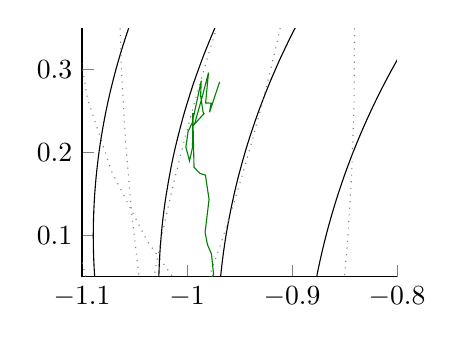
\begin{tikzpicture}

\begin{axis}[%
width=4cm,
height=3.15483870967742cm,
colormap={mymap}{[1pt] rgb(0pt)=(0,0,0); rgb(1pt)=(0,0,0)},
unbounded coords=jump,
scale only axis,
xmin=-1.1,
xmax=-0.8,
ymin=0.05,
ymax=0.35,
axis x line*=bottom,
axis y line*=left
]

\addplot[area legend,solid,draw=black,forget plot]
table[row sep=crcr]{
x y\\
-1.23 0.46490355595815 \\
-1.22960150659877 0.47 \\
-1.22869862032926 0.48 \\
-1.22767371065223 0.49 \\
-1.22652615959779 0.5 \\
-1.22525527442296 0.51 \\
-1.22386028691466 0.52 \\
-1.22234035261571 0.53 \\
-1.22069454997284 0.54 \\
-1.22 0.543925012252854 \\
-1.21892640279752 0.55 \\
-1.21703375996655 0.56 \\
-1.21501255351594 0.57 \\
-1.21286154858517 0.58 \\
-1.21057942808711 0.59 \\
-1.21 0.592406769213231 \\
-1.20817185045267 0.6 \\
-1.20563301512456 0.61 \\
-1.20295912720575 0.62 \\
-1.2001485327529 0.63 \\
-1.2 0.630505916752702 \\
-1.19720927177399 0.64 \\
-1.19413073501926 0.65 \\
-1.19091048235894 0.66 \\
-1.19 0.662717034143122 \\
-1.18755419286408 0.67 \\
-1.1840553713141 0.68 \\
-1.18040895669849 0.69 \\
-1.18 0.691082930921102 \\
-1.1766220430266 0.7 \\
-1.17268437715587 0.71 \\
-1.17 0.716574164360218 \\
-1.16859570678079 0.72 \\
-1.16435686868754 0.73 \\
-1.16 0.739906655398264 \\
-1.15995875610125 0.74 \\
-1.15540766506219 0.75 \\
-1.15069176174176 0.76 \\
-1.15 0.76142534514183 \\
-1.14581495754822 0.77 \\
-1.14076851906906 0.78 \\
-1.14 0.781481800290595 \\
-1.13555370431776 0.79 \\
-1.13016256518617 0.8 \\
-1.13 0.800294055571771 \\
-1.12459541368304 0.81 \\
-1.12 0.818003330802316 \\
-1.11884457213804 0.82 \\
-1.11290789864718 0.83 \\
-1.11 0.834766310779763 \\
-1.1067794262609 0.84 \\
-1.10045499989146 0.85 \\
-1.1 0.85070324293253 \\
-1.09392825155636 0.86 \\
-1.09 0.86585779537492 \\
-1.08719432959242 0.87 \\
-1.0802478170049 0.88 \\
-1.08 0.880349311626938 \\
-1.07307898957916 0.89 \\
-1.07 0.894191086141864 \\
-1.06568343026022 0.9 \\
-1.06 0.907472179329761 \\
-1.0580539964072 0.91 \\
-1.05018227493588 0.92 \\
-1.05 0.920227114822055 \\
-1.0420548844932 0.93 \\
-1.04 0.932474665837886 \\
-1.0336661072561 0.94 \\
-1.03 0.944267684379233 \\
-1.02500542583447 0.95 \\
-1.02 0.955632804221174 \\
-1.01606124067785 0.96 \\
-1.01 0.96659434215035 \\
-1.00682078403302 0.97 \\
-1 0.977174502586599 \\
-0.997270024404195 0.98 \\
-0.99 0.987393560386835 \\
-0.987393560386835 0.99 \\
-0.98 0.997270024404194 \\
-0.977174502586599 1 \\
-0.97 1.00682078403302 \\
-0.96659434215035 1.01 \\
-0.96 1.01606124067785 \\
-0.955632804221174 1.02 \\
-0.95 1.02500542583447 \\
-0.944267684379233 1.03 \\
-0.94 1.0336661072561 \\
-0.932474665837887 1.04 \\
-0.93 1.0420548844932 \\
-0.920227114822055 1.05 \\
-0.92 1.05018227493588 \\
-0.91 1.0580539964072 \\
-0.90747217932976 1.06 \\
-0.9 1.06568343026022 \\
-0.894191086141864 1.07 \\
-0.89 1.07307898957916 \\
-0.880349311626938 1.08 \\
-0.88 1.0802478170049 \\
-0.87 1.08719432959242 \\
-0.86585779537492 1.09 \\
-0.86 1.09392825155636 \\
-0.85070324293253 1.1 \\
-0.85 1.10045499989146 \\
-0.84 1.1067794262609 \\
-0.834766310779763 1.11 \\
-0.83 1.11290789864718 \\
-0.82 1.11884457213804 \\
-0.818003330802316 1.12 \\
-0.81 1.12459541368304 \\
-0.800294055571771 1.13 \\
-0.8 1.13016256518617 \\
-0.79 1.13555370431776 \\
-0.781481800290595 1.14 \\
-0.78 1.14076851906906 \\
-0.77 1.14581495754822 \\
-0.76142534514183 1.15 \\
-0.76 1.15069176174176 \\
-0.75 1.15540766506219 \\
-0.74 1.15995875610125 \\
-0.739906655398264 1.16 \\
-0.73 1.16435686868754 \\
-0.72 1.16859570678079 \\
-0.716574164360217 1.17 \\
-0.71 1.17268437715587 \\
-0.7 1.1766220430266 \\
-0.691082930921101 1.18 \\
-0.69 1.18040895669849 \\
-0.68 1.1840553713141 \\
-0.67 1.18755419286408 \\
-0.662717034143123 1.19 \\
-0.66 1.19091048235894 \\
-0.65 1.19413073501926 \\
-0.64 1.19720927177399 \\
-0.630505916752703 1.2 \\
-0.63 1.2001485327529 \\
-0.62 1.20295912720575 \\
-0.61 1.20563301512456 \\
-0.6 1.20817185045267 \\
-0.592406769213231 1.21 \\
-0.59 1.21057942808711 \\
-0.58 1.21286154858517 \\
-0.57 1.21501255351594 \\
-0.56 1.21703375996655 \\
-0.55 1.21892640279752 \\
-0.543925012252854 1.22 \\
-0.54 1.22069454997284 \\
-0.53 1.22234035261571 \\
-0.52 1.22386028691466 \\
-0.51 1.22525527442296 \\
-0.5 1.22652615959779 \\
-0.49 1.22767371065223 \\
-0.48 1.22869862032926 \\
-0.47 1.22960150659877 \\
-0.46490355595815 1.23 \\
-0.46 1.23038466003635 \\
-0.45 1.23104806991097 \\
-0.44 1.23159031728077 \\
-0.43 1.23201172796599 \\
-0.42 1.23231255504488 \\
-0.41 1.23249297910695 \\
-0.4 1.2325531084337 \\
-0.39 1.23249297910695 \\
-0.38 1.23231255504488 \\
-0.37 1.23201172796599 \\
-0.36 1.23159031728077 \\
-0.35 1.23104806991097 \\
-0.34 1.23038466003635 \\
-0.335096444041851 1.23 \\
-0.33 1.22960150659877 \\
-0.32 1.22869862032926 \\
-0.31 1.22767371065223 \\
-0.3 1.22652615959779 \\
-0.29 1.22525527442296 \\
-0.28 1.22386028691466 \\
-0.27 1.22234035261571 \\
-0.26 1.22069454997284 \\
-0.256074987747147 1.22 \\
-0.25 1.21892640279752 \\
-0.24 1.21703375996655 \\
-0.23 1.21501255351594 \\
-0.22 1.21286154858517 \\
-0.21 1.21057942808711 \\
-0.207593230786769 1.21 \\
-0.2 1.20817185045267 \\
-0.19 1.20563301512456 \\
-0.18 1.20295912720575 \\
-0.17 1.2001485327529 \\
-0.169494083247298 1.2 \\
-0.16 1.19720927177399 \\
-0.15 1.19413073501926 \\
-0.14 1.19091048235894 \\
-0.137282965856877 1.19 \\
-0.13 1.18755419286408 \\
-0.12 1.1840553713141 \\
-0.11 1.18040895669849 \\
-0.108917069078899 1.18 \\
-0.0999999999999999 1.1766220430266 \\
-0.0899999999999999 1.17268437715587 \\
-0.0834258356397825 1.17 \\
-0.0800000000000001 1.16859570678079 \\
-0.0700000000000001 1.16435686868754 \\
-0.0600933446017362 1.16 \\
-0.0600000000000001 1.15995875610125 \\
-0.05 1.15540766506219 \\
-0.04 1.15069176174176 \\
-0.0385746548581699 1.15 \\
-0.03 1.14581495754822 \\
-0.02 1.14076851906906 \\
-0.0185181997094054 1.14 \\
-0.01 1.13555370431776 \\
0 1.13016256518617 \\
0.000294055571771424 1.13 \\
0.01 1.12459541368304 \\
0.0180033308023158 1.12 \\
0.02 1.11884457213804 \\
0.03 1.11290789864718 \\
0.0347663107797624 1.11 \\
0.04 1.1067794262609 \\
0.05 1.10045499989146 \\
0.0507032429325301 1.1 \\
0.0600000000000001 1.09392825155636 \\
0.0658577953749194 1.09 \\
0.0700000000000001 1.08719432959242 \\
0.0800000000000001 1.0802478170049 \\
0.0803493116269377 1.08 \\
0.0899999999999999 1.07307898957916 \\
0.0941910861418636 1.07 \\
0.0999999999999999 1.06568343026022 \\
0.10747217932976 1.06 \\
0.11 1.0580539964072 \\
0.12 1.05018227493588 \\
0.120227114822055 1.05 \\
0.13 1.0420548844932 \\
0.132474665837886 1.04 \\
0.14 1.0336661072561 \\
0.144267684379233 1.03 \\
0.15 1.02500542583447 \\
0.155632804221174 1.02 \\
0.16 1.01606124067785 \\
0.16659434215035 1.01 \\
0.17 1.00682078403302 \\
0.1771745025866 1 \\
0.18 0.997270024404194 \\
0.187393560386835 0.99 \\
0.19 0.987393560386835 \\
0.197270024404195 0.98 \\
0.2 0.977174502586599 \\
0.206820784033018 0.97 \\
0.21 0.96659434215035 \\
0.216061240677853 0.96 \\
0.22 0.955632804221174 \\
0.225005425834474 0.95 \\
0.23 0.944267684379233 \\
0.233666107256098 0.94 \\
0.24 0.932474665837886 \\
0.242054884493204 0.93 \\
0.25 0.920227114822055 \\
0.250182274935881 0.92 \\
0.258053996407202 0.91 \\
0.26 0.907472179329761 \\
0.265683430260224 0.9 \\
0.27 0.894191086141863 \\
0.273078989579159 0.89 \\
0.28 0.880349311626938 \\
0.280247817004903 0.88 \\
0.287194329592418 0.87 \\
0.29 0.865857795374919 \\
0.293928251556358 0.86 \\
0.3 0.85070324293253 \\
0.300454999891464 0.85 \\
0.306779426260899 0.84 \\
0.31 0.834766310779762 \\
0.312907898647181 0.83 \\
0.318844572138043 0.82 \\
0.32 0.818003330802316 \\
0.324595413683044 0.81 \\
0.33 0.800294055571771 \\
0.330162565186173 0.8 \\
0.335553704317761 0.79 \\
0.34 0.781481800290595 \\
0.340768519069056 0.78 \\
0.345814957548218 0.77 \\
0.35 0.76142534514183 \\
0.350691761741762 0.76 \\
0.355407665062195 0.75 \\
0.359958756101252 0.74 \\
0.36 0.739906655398264 \\
0.364356868687543 0.73 \\
0.368595706780788 0.72 \\
0.37 0.716574164360218 \\
0.372684377155872 0.71 \\
0.376622043026596 0.7 \\
0.38 0.691082930921102 \\
0.380408956698492 0.69 \\
0.384055371314095 0.68 \\
0.387554192864077 0.67 \\
0.39 0.662717034143122 \\
0.390910482358941 0.66 \\
0.394130735019259 0.65 \\
0.397209271773994 0.64 \\
0.4 0.630505916752702 \\
0.400148532752897 0.63 \\
0.402959127205753 0.62 \\
0.405633015124562 0.61 \\
0.408171850452672 0.6 \\
0.41 0.592406769213231 \\
0.410579428087114 0.59 \\
0.41286154858517 0.58 \\
0.415012553515935 0.57 \\
0.417033759966547 0.56 \\
0.418926402797516 0.55 \\
0.42 0.543925012252854 \\
0.420694549972838 0.54 \\
0.422340352615714 0.53 \\
0.423860286914664 0.52 \\
0.425255274422965 0.51 \\
0.426526159597789 0.5 \\
0.427673710652226 0.49 \\
0.428698620329256 0.48 \\
0.429601506598767 0.47 \\
0.43 0.46490355595815 \\
0.430384660036347 0.46 \\
0.431048069910975 0.45 \\
0.431590317280767 0.44 \\
0.432011727965991 0.43 \\
0.432312555044877 0.42 \\
0.432492979106945 0.41 \\
0.432553108433699 0.4 \\
0.432492979106945 0.39 \\
0.432312555044877 0.38 \\
0.432011727965991 0.37 \\
0.431590317280767 0.36 \\
0.431048069910975 0.35 \\
0.430384660036347 0.34 \\
0.43 0.335096444041851 \\
0.429601506598767 0.33 \\
0.428698620329256 0.32 \\
0.427673710652226 0.31 \\
0.426526159597789 0.3 \\
0.425255274422965 0.29 \\
0.423860286914664 0.28 \\
0.422340352615714 0.27 \\
0.420694549972838 0.26 \\
0.42 0.256074987747147 \\
0.418926402797516 0.25 \\
0.417033759966547 0.24 \\
0.415012553515935 0.23 \\
0.41286154858517 0.22 \\
0.410579428087114 0.21 \\
0.41 0.207593230786769 \\
0.408171850452672 0.2 \\
0.405633015124562 0.19 \\
0.402959127205753 0.18 \\
0.400148532752897 0.17 \\
0.4 0.169494083247298 \\
0.397209271773994 0.16 \\
0.394130735019258 0.15 \\
0.390910482358941 0.14 \\
0.39 0.137282965856877 \\
0.387554192864077 0.13 \\
0.384055371314095 0.12 \\
0.380408956698492 0.11 \\
0.38 0.108917069078899 \\
0.376622043026596 0.0999999999999999 \\
0.372684377155872 0.0899999999999999 \\
0.37 0.0834258356397825 \\
0.368595706780788 0.0800000000000001 \\
0.364356868687543 0.0700000000000001 \\
0.36 0.0600933446017357 \\
0.359958756101252 0.0600000000000001 \\
0.355407665062195 0.05 \\
0.350691761741762 0.04 \\
0.35 0.0385746548581699 \\
0.345814957548218 0.03 \\
0.340768519069056 0.02 \\
0.34 0.0185181997094054 \\
0.335553704317761 0.01 \\
0.330162565186173 0 \\
0.33 -0.000294055571771139 \\
0.324595413683044 -0.01 \\
0.32 -0.0180033308023158 \\
0.318844572138043 -0.02 \\
0.312907898647181 -0.03 \\
0.31 -0.0347663107797621 \\
0.306779426260899 -0.04 \\
0.300454999891464 -0.05 \\
0.3 -0.0507032429325301 \\
0.293928251556357 -0.0600000000000001 \\
0.29 -0.0658577953749191 \\
0.287194329592418 -0.0700000000000001 \\
0.280247817004903 -0.0800000000000001 \\
0.28 -0.0803493116269377 \\
0.273078989579159 -0.0899999999999999 \\
0.27 -0.0941910861418633 \\
0.265683430260224 -0.0999999999999999 \\
0.26 -0.10747217932976 \\
0.258053996407202 -0.11 \\
0.250182274935881 -0.12 \\
0.25 -0.120227114822055 \\
0.242054884493204 -0.13 \\
0.24 -0.132474665837886 \\
0.233666107256098 -0.14 \\
0.23 -0.144267684379233 \\
0.225005425834474 -0.15 \\
0.22 -0.155632804221174 \\
0.216061240677853 -0.16 \\
0.21 -0.16659434215035 \\
0.206820784033018 -0.17 \\
0.2 -0.1771745025866 \\
0.197270024404195 -0.18 \\
0.19 -0.187393560386835 \\
0.187393560386835 -0.19 \\
0.18 -0.197270024404195 \\
0.1771745025866 -0.2 \\
0.17 -0.206820784033018 \\
0.16659434215035 -0.21 \\
0.16 -0.216061240677853 \\
0.155632804221174 -0.22 \\
0.15 -0.225005425834474 \\
0.144267684379233 -0.23 \\
0.14 -0.233666107256098 \\
0.132474665837886 -0.24 \\
0.13 -0.242054884493204 \\
0.120227114822055 -0.25 \\
0.12 -0.250182274935881 \\
0.11 -0.258053996407202 \\
0.10747217932976 -0.26 \\
0.0999999999999999 -0.265683430260224 \\
0.0941910861418633 -0.27 \\
0.0899999999999999 -0.273078989579159 \\
0.0803493116269377 -0.28 \\
0.0800000000000001 -0.280247817004903 \\
0.0700000000000001 -0.287194329592418 \\
0.0658577953749191 -0.29 \\
0.0600000000000001 -0.293928251556357 \\
0.0507032429325301 -0.3 \\
0.05 -0.300454999891464 \\
0.04 -0.306779426260899 \\
0.0347663107797621 -0.31 \\
0.03 -0.312907898647181 \\
0.02 -0.318844572138043 \\
0.0180033308023158 -0.32 \\
0.01 -0.324595413683044 \\
0.000294055571771139 -0.33 \\
0 -0.330162565186173 \\
-0.01 -0.335553704317761 \\
-0.0185181997094054 -0.34 \\
-0.02 -0.340768519069056 \\
-0.03 -0.345814957548218 \\
-0.0385746548581699 -0.35 \\
-0.04 -0.350691761741762 \\
-0.05 -0.355407665062195 \\
-0.0600000000000001 -0.359958756101252 \\
-0.0600933446017357 -0.36 \\
-0.0700000000000001 -0.364356868687543 \\
-0.0800000000000001 -0.368595706780788 \\
-0.0834258356397825 -0.37 \\
-0.0899999999999999 -0.372684377155872 \\
-0.0999999999999999 -0.376622043026596 \\
-0.108917069078899 -0.38 \\
-0.11 -0.380408956698492 \\
-0.12 -0.384055371314095 \\
-0.13 -0.387554192864077 \\
-0.137282965856877 -0.39 \\
-0.14 -0.390910482358941 \\
-0.15 -0.394130735019258 \\
-0.16 -0.397209271773994 \\
-0.169494083247298 -0.4 \\
-0.17 -0.400148532752897 \\
-0.18 -0.402959127205753 \\
-0.19 -0.405633015124562 \\
-0.2 -0.408171850452672 \\
-0.207593230786769 -0.41 \\
-0.21 -0.410579428087114 \\
-0.22 -0.41286154858517 \\
-0.23 -0.415012553515935 \\
-0.24 -0.417033759966547 \\
-0.25 -0.418926402797516 \\
-0.256074987747147 -0.42 \\
-0.26 -0.420694549972838 \\
-0.27 -0.422340352615714 \\
-0.28 -0.423860286914664 \\
-0.29 -0.425255274422965 \\
-0.3 -0.426526159597789 \\
-0.31 -0.427673710652226 \\
-0.32 -0.428698620329256 \\
-0.33 -0.429601506598767 \\
-0.335096444041851 -0.43 \\
-0.34 -0.430384660036347 \\
-0.35 -0.431048069910975 \\
-0.36 -0.431590317280767 \\
-0.37 -0.432011727965991 \\
-0.38 -0.432312555044877 \\
-0.39 -0.432492979106945 \\
-0.4 -0.432553108433699 \\
-0.41 -0.432492979106945 \\
-0.42 -0.432312555044877 \\
-0.43 -0.432011727965991 \\
-0.44 -0.431590317280767 \\
-0.45 -0.431048069910975 \\
-0.46 -0.430384660036347 \\
-0.46490355595815 -0.43 \\
-0.47 -0.429601506598767 \\
-0.48 -0.428698620329256 \\
-0.49 -0.427673710652226 \\
-0.5 -0.426526159597789 \\
-0.51 -0.425255274422965 \\
-0.52 -0.423860286914664 \\
-0.53 -0.422340352615714 \\
-0.54 -0.420694549972838 \\
-0.543925012252854 -0.42 \\
-0.55 -0.418926402797516 \\
-0.56 -0.417033759966547 \\
-0.57 -0.415012553515935 \\
-0.58 -0.41286154858517 \\
-0.59 -0.410579428087114 \\
-0.592406769213231 -0.41 \\
-0.6 -0.408171850452672 \\
-0.61 -0.405633015124562 \\
-0.62 -0.402959127205753 \\
-0.63 -0.400148532752897 \\
-0.630505916752703 -0.4 \\
-0.64 -0.397209271773994 \\
-0.65 -0.394130735019259 \\
-0.66 -0.390910482358941 \\
-0.662717034143123 -0.39 \\
-0.67 -0.387554192864077 \\
-0.68 -0.384055371314095 \\
-0.69 -0.380408956698492 \\
-0.691082930921101 -0.38 \\
-0.7 -0.376622043026596 \\
-0.71 -0.372684377155872 \\
-0.716574164360217 -0.37 \\
-0.72 -0.368595706780788 \\
-0.73 -0.364356868687543 \\
-0.739906655398264 -0.36 \\
-0.74 -0.359958756101252 \\
-0.75 -0.355407665062195 \\
-0.76 -0.350691761741762 \\
-0.76142534514183 -0.35 \\
-0.77 -0.345814957548218 \\
-0.78 -0.340768519069056 \\
-0.781481800290595 -0.34 \\
-0.79 -0.335553704317761 \\
-0.8 -0.330162565186173 \\
-0.800294055571771 -0.33 \\
-0.81 -0.324595413683044 \\
-0.818003330802316 -0.32 \\
-0.82 -0.318844572138043 \\
-0.83 -0.312907898647181 \\
-0.834766310779762 -0.31 \\
-0.84 -0.306779426260899 \\
-0.85 -0.300454999891464 \\
-0.85070324293253 -0.3 \\
-0.86 -0.293928251556358 \\
-0.865857795374919 -0.29 \\
-0.87 -0.287194329592418 \\
-0.88 -0.280247817004903 \\
-0.880349311626938 -0.28 \\
-0.89 -0.273078989579159 \\
-0.894191086141863 -0.27 \\
-0.9 -0.265683430260224 \\
-0.90747217932976 -0.26 \\
-0.91 -0.258053996407202 \\
-0.92 -0.250182274935881 \\
-0.920227114822055 -0.25 \\
-0.93 -0.242054884493204 \\
-0.932474665837887 -0.24 \\
-0.94 -0.233666107256098 \\
-0.944267684379233 -0.23 \\
-0.95 -0.225005425834474 \\
-0.955632804221174 -0.22 \\
-0.96 -0.216061240677853 \\
-0.96659434215035 -0.21 \\
-0.97 -0.206820784033018 \\
-0.977174502586599 -0.2 \\
-0.98 -0.197270024404195 \\
-0.987393560386835 -0.19 \\
-0.99 -0.187393560386835 \\
-0.997270024404195 -0.18 \\
-1 -0.1771745025866 \\
-1.00682078403302 -0.17 \\
-1.01 -0.16659434215035 \\
-1.01606124067785 -0.16 \\
-1.02 -0.155632804221174 \\
-1.02500542583447 -0.15 \\
-1.03 -0.144267684379233 \\
-1.0336661072561 -0.14 \\
-1.04 -0.132474665837886 \\
-1.0420548844932 -0.13 \\
-1.05 -0.120227114822055 \\
-1.05018227493588 -0.12 \\
-1.0580539964072 -0.11 \\
-1.06 -0.10747217932976 \\
-1.06568343026022 -0.0999999999999999 \\
-1.07 -0.0941910861418636 \\
-1.07307898957916 -0.0899999999999999 \\
-1.08 -0.0803493116269377 \\
-1.0802478170049 -0.0800000000000001 \\
-1.08719432959242 -0.0700000000000001 \\
-1.09 -0.0658577953749194 \\
-1.09392825155636 -0.0600000000000001 \\
-1.1 -0.0507032429325301 \\
-1.10045499989146 -0.05 \\
-1.1067794262609 -0.04 \\
-1.11 -0.0347663107797624 \\
-1.11290789864718 -0.03 \\
-1.11884457213804 -0.02 \\
-1.12 -0.0180033308023158 \\
-1.12459541368304 -0.01 \\
-1.13 -0.000294055571771424 \\
-1.13016256518617 0 \\
-1.13555370431776 0.01 \\
-1.14 0.0185181997094054 \\
-1.14076851906906 0.02 \\
-1.14581495754822 0.03 \\
-1.15 0.0385746548581699 \\
-1.15069176174176 0.04 \\
-1.15540766506219 0.05 \\
-1.15995875610125 0.0600000000000001 \\
-1.16 0.0600933446017362 \\
-1.16435686868754 0.0700000000000001 \\
-1.16859570678079 0.0800000000000001 \\
-1.17 0.0834258356397825 \\
-1.17268437715587 0.0899999999999999 \\
-1.1766220430266 0.0999999999999999 \\
-1.18 0.108917069078899 \\
-1.18040895669849 0.11 \\
-1.1840553713141 0.12 \\
-1.18755419286408 0.13 \\
-1.19 0.137282965856877 \\
-1.19091048235894 0.14 \\
-1.19413073501926 0.15 \\
-1.19720927177399 0.16 \\
-1.2 0.169494083247298 \\
-1.2001485327529 0.17 \\
-1.20295912720575 0.18 \\
-1.20563301512456 0.19 \\
-1.20817185045267 0.2 \\
-1.21 0.207593230786769 \\
-1.21057942808711 0.21 \\
-1.21286154858517 0.22 \\
-1.21501255351594 0.23 \\
-1.21703375996655 0.24 \\
-1.21892640279752 0.25 \\
-1.22 0.256074987747147 \\
-1.22069454997284 0.26 \\
-1.22234035261571 0.27 \\
-1.22386028691466 0.28 \\
-1.22525527442296 0.29 \\
-1.22652615959779 0.3 \\
-1.22767371065223 0.31 \\
-1.22869862032926 0.32 \\
-1.22960150659877 0.33 \\
-1.23 0.335096444041851 \\
-1.23038466003635 0.34 \\
-1.23104806991097 0.35 \\
-1.23159031728077 0.36 \\
-1.23201172796599 0.37 \\
-1.23231255504488 0.38 \\
-1.23249297910694 0.39 \\
-1.2325531084337 0.4 \\
-1.23249297910694 0.41 \\
-1.23231255504488 0.42 \\
-1.23201172796599 0.43 \\
-1.23159031728077 0.44 \\
-1.23104806991097 0.45 \\
-1.23038466003635 0.46 \\
-1.23 0.46490355595815 \\
NaN NaN \\
};

\addplot [
color=gray,
dotted,
forget plot
]
table[row sep=crcr]{
0.302858053669543 0.4\\
0.29706717591351 0.490422808186003\\
0.279789628698068 0.579360876361465\\
0.25130910887083 0.665353843905771\\
0.212093265779973 0.746989708669247\\
0.162786022484869 0.822928012009422\\
0.104197002557251 0.891921849084879\\
0.0372882360845491 0.952838342998275\\
-0.0368416368375469 1.00467724660368\\
-0.116975405745088 1.04658736653706\\
-0.201797276368028 1.07788053978777\\
-0.289914475935768 1.09804293331619\\
-0.379880122467536 1.10674348117799\\
-0.470216982534515 1.10383932061783\\
-0.559441727391902 1.08937813787181\\
-0.64608928919589 1.06359738516082\\
-0.72873691737716 1.02692038173164\\
-0.806027540165891 0.979949362966567\\
-0.876692047672707 0.923455591695151\\
-0.939570130637972 0.858366694079811\\
-0.993629332677755 0.785751428019912\\
-1.03798200318911 0.7068021341766\\
-1.07189987254844 0.622815157772112\\
-1.09482601027856 0.535169562637062\\
-1.10638396983179 0.445304487020476\\
-1.10638396983179 0.354695512979524\\
-1.09482601027856 0.264830437362938\\
-1.07189987254844 0.177184842227889\\
-1.03798200318911 0.0931978658233998\\
-0.993629332677756 0.0142485719800879\\
-0.939570130637972 -0.058366694079811\\
-0.876692047672707 -0.123455591695151\\
-0.806027540165891 -0.179949362966567\\
-0.72873691737716 -0.226920381731638\\
-0.64608928919589 -0.263597385160825\\
-0.559441727391902 -0.28937813787181\\
-0.470216982534514 -0.303839320617828\\
-0.379880122467536 -0.30674348117799\\
-0.289914475935769 -0.298042933316187\\
-0.201797276368029 -0.277880539787771\\
-0.116975405745088 -0.246587366537059\\
-0.0368416368375474 -0.204677246603681\\
0.037288236084549 -0.152838342998275\\
0.10419700255725 -0.0919218490848791\\
0.162786022484868 -0.0229280120094228\\
0.212093265779973 0.0530102913307532\\
0.25130910887083 0.134646156094229\\
0.279789628698068 0.220639123638535\\
0.29706717591351 0.309577191813997\\
0.302858053669543 0.4\\
};

\addplot[area legend,solid,draw=black,forget plot]
table[row sep=crcr]{
x y\\
-1.17 0.34824483234669 \\
-1.16974685063192 0.35 \\
-1.16819226362119 0.36 \\
-1.16652579083749 0.37 \\
-1.16474640465062 0.38 \\
-1.16285290186727 0.39 \\
-1.16084389340103 0.4 \\
-1.16 0.403972283004096 \\
-1.15872752024962 0.41 \\
-1.15650161857746 0.42 \\
-1.15415850992452 0.43 \\
-1.15169620345948 0.44 \\
-1.15 0.446570497508841 \\
-1.14911957270876 0.45 \\
-1.14643582378503 0.46 \\
-1.14362995065294 0.47 \\
-1.14069920346947 0.48 \\
-1.14 0.482292669864651 \\
-1.13766087050511 0.49 \\
-1.13450203673762 0.5 \\
-1.13121376409444 0.51 \\
-1.13 0.513558350248353 \\
-1.1278116203584 0.52 \\
-1.12428796612075 0.53 \\
-1.12062893201116 0.54 \\
-1.12 0.541663477723823 \\
-1.11685840800488 0.55 \\
-1.11295502020046 0.56 \\
-1.11 0.56731503463497 \\
-1.1089179667055 0.57 \\
-1.10476285025168 0.58 \\
-1.10046101620946 0.59 \\
-1.1 0.591041770839401 \\
-1.09604227319328 0.6 \\
-1.09147623443274 0.61 \\
-1.09 0.613142166756836 \\
-1.08678076273977 0.62 \\
-1.08194080954232 0.63 \\
-1.08 0.633899158806308 \\
-1.07696335112985 0.64 \\
-1.07183867003779 0.65 \\
-1.07 0.653493256137173 \\
-1.06657249843507 0.66 \\
-1.06115098587887 0.67 \\
-1.06 0.672071557680547 \\
-1.05558789116181 0.68 \\
-1.05 0.689751052742826 \\
-1.04985699636204 0.69 \\
-1.04398616547374 0.7 \\
-1.04 0.706603959589081 \\
-1.03794361838801 0.71 \\
-1.03174054970386 0.72 \\
-1.03 0.722741706044418 \\
-1.02537385112673 0.73 \\
-1.02 0.738216777058695 \\
-1.01882821800339 0.74 \\
-1.01211523648097 0.75 \\
-1.01 0.753080756290404 \\
-1.00522296955145 0.76 \\
-1 0.767388077842723 \\
-0.998141887321532 0.77 \\
-0.990874145928976 0.78 \\
-0.99 0.781179799014672 \\
-0.983418455088601 0.79 \\
-0.98 0.794483082457343 \\
-0.975760203119438 0.8 \\
-0.97 0.807340585135123 \\
-0.967895220180388 0.81 \\
-0.96 0.819777404251693 \\
-0.959818579796784 0.82 \\
-0.951530102936964 0.83 \\
-0.95 0.831812067722366 \\
-0.943015865809287 0.84 \\
-0.94 0.843472184497663 \\
-0.934268290314526 0.85 \\
-0.93 0.854777416654995 \\
-0.925279730157293 0.86 \\
-0.92 0.865745241610559 \\
-0.916041674018024 0.87 \\
-0.91 0.876391723329543 \\
-0.906544708951422 0.88 \\
-0.9 0.886731619659182 \\
-0.896778476336056 0.89 \\
-0.89 0.896778476336056 \\
-0.886731619659182 0.9 \\
-0.88 0.906544708951422 \\
-0.876391723329543 0.91 \\
-0.87 0.916041674018024 \\
-0.865745241610559 0.92 \\
-0.86 0.925279730157293 \\
-0.854777416654995 0.93 \\
-0.85 0.934268290314526 \\
-0.843472184497663 0.94 \\
-0.84 0.943015865809288 \\
-0.831812067722366 0.95 \\
-0.83 0.951530102936965 \\
-0.82 0.959818579796784 \\
-0.819777404251693 0.96 \\
-0.81 0.967895220180388 \\
-0.807340585135122 0.97 \\
-0.8 0.975760203119437 \\
-0.794483082457343 0.98 \\
-0.79 0.983418455088602 \\
-0.781179799014672 0.99 \\
-0.78 0.990874145928976 \\
-0.77 0.998141887321532 \\
-0.767388077842723 1 \\
-0.76 1.00522296955145 \\
-0.753080756290404 1.01 \\
-0.75 1.01211523648097 \\
-0.74 1.01882821800339 \\
-0.738216777058696 1.02 \\
-0.73 1.02537385112673 \\
-0.722741706044418 1.03 \\
-0.72 1.03174054970386 \\
-0.71 1.03794361838801 \\
-0.706603959589081 1.04 \\
-0.7 1.04398616547375 \\
-0.69 1.04985699636204 \\
-0.689751052742826 1.05 \\
-0.68 1.05558789116181 \\
-0.672071557680547 1.06 \\
-0.67 1.06115098587887 \\
-0.66 1.06657249843507 \\
-0.653493256137172 1.07 \\
-0.65 1.07183867003779 \\
-0.64 1.07696335112985 \\
-0.633899158806308 1.08 \\
-0.63 1.08194080954232 \\
-0.62 1.08678076273977 \\
-0.613142166756836 1.09 \\
-0.61 1.09147623443274 \\
-0.6 1.09604227319328 \\
-0.591041770839401 1.1 \\
-0.59 1.10046101620946 \\
-0.58 1.10476285025168 \\
-0.57 1.1089179667055 \\
-0.56731503463497 1.11 \\
-0.56 1.11295502020045 \\
-0.55 1.11685840800488 \\
-0.541663477723823 1.12 \\
-0.54 1.12062893201116 \\
-0.53 1.12428796612075 \\
-0.52 1.1278116203584 \\
-0.513558350248353 1.13 \\
-0.51 1.13121376409444 \\
-0.5 1.13450203673762 \\
-0.49 1.13766087050511 \\
-0.482292669864651 1.14 \\
-0.48 1.14069920346947 \\
-0.47 1.14362995065294 \\
-0.46 1.14643582378503 \\
-0.45 1.14911957270876 \\
-0.446570497508841 1.15 \\
-0.44 1.15169620345948 \\
-0.43 1.15415850992452 \\
-0.42 1.15650161857746 \\
-0.41 1.15872752024962 \\
-0.403972283004096 1.16 \\
-0.4 1.16084389340103 \\
-0.39 1.16285290186727 \\
-0.38 1.16474640465062 \\
-0.37 1.16652579083749 \\
-0.36 1.16819226362119 \\
-0.35 1.16974685063192 \\
-0.34824483234669 1.17 \\
-0.34 1.17119736332875 \\
-0.33 1.17253708306572 \\
-0.32 1.17376516554583 \\
-0.31 1.17488223536639 \\
-0.3 1.17588878364361 \\
-0.29 1.17678517647896 \\
-0.28 1.17757166314514 \\
-0.27 1.17824838400104 \\
-0.26 1.17881537814023 \\
-0.25 1.17927259077445 \\
-0.24 1.17961988034923 \\
-0.23 1.1798570253855 \\
-0.22 1.17998373103776 \\
-0.21 1.17999963535578 \\
-0.2 1.17990431523439 \\
-0.19 1.17969729203277 \\
-0.18 1.17937803684251 \\
-0.17 1.17894597538143 \\
-0.16 1.17840049248854 \\
-0.15 1.17774093619399 \\
-0.14 1.1769666213368 \\
-0.13 1.17607683270263 \\
-0.12 1.17507082765349 \\
-0.11 1.17394783822133 \\
-0.0999999999999999 1.17270707263833 \\
-0.0899999999999999 1.17134771627709 \\
-0.0808808221553111 1.17 \\
-0.0800000000000001 1.169868446055 \\
-0.0700000000000001 1.16826318492631 \\
-0.0600000000000001 1.1665358522753 \\
-0.05 1.16468558953898 \\
-0.04 1.16271152558355 \\
-0.03 1.16061277372685 \\
-0.0272297162274458 1.16 \\
-0.02 1.15837707043464 \\
-0.01 1.15600950424899 \\
0 1.15351353518583 \\
0.01 1.15088831903331 \\
0.0132417961451759 1.15 \\
0.02 1.1481144843506 \\
0.03 1.1451998014171 \\
0.04 1.14215236860539 \\
0.0467845809778874 1.14 \\
0.05 1.13895839590464 \\
0.0600000000000001 1.13560172760492 \\
0.0700000000000001 1.13210924568362 \\
0.0758326192762357 1.13 \\
0.0800000000000001 1.12845705211644 \\
0.0899999999999999 1.12463447377779 \\
0.0999999999999999 1.12067372352401 \\
0.101654875861228 1.12 \\
0.11 1.11651329321956 \\
0.12 1.11220142977958 \\
0.124965625555616 1.11 \\
0.13 1.10770379085866 \\
0.14 1.10302068977659 \\
0.146281627658991 1.1 \\
0.15 1.09815606221167 \\
0.16 1.09308122969512 \\
0.165927999060679 1.09 \\
0.17 1.08781244454026 \\
0.18 1.08232554760214 \\
0.18415237085094 1.08 \\
0.19 1.07660791404929 \\
0.2 1.07068940384791 \\
0.201145721652617 1.07 \\
0.21 1.06447069599288 \\
0.217032177449418 1.06 \\
0.22 1.05803665457619 \\
0.23 1.05132313374821 \\
0.231943882101265 1.05 \\
0.24 1.04428372571177 \\
0.245958520328016 1.04 \\
0.25 1.03696310983243 \\
0.259164215758356 1.03 \\
0.26 1.02933444169534 \\
0.27 1.02130039326315 \\
0.27160451321306 1.02 \\
0.28 1.01285817275248 \\
0.283336244087455 1.01 \\
0.29 1.0039916294524 \\
0.29440365869371 1 \\
0.3 0.994646303613179 \\
0.30483949801983 0.99 \\
0.31 0.984756110397065 \\
0.314671396184423 0.98 \\
0.32 0.974240900702571 \\
0.323922474439262 0.97 \\
0.33 0.963003381220004 \\
0.332611869145027 0.96 \\
0.34 0.950925197880764 \\
0.340755206485876 0.95 \\
0.348353919103909 0.94 \\
0.35 0.937660090845779 \\
0.355419004395882 0.93 \\
0.36 0.922984220900905 \\
0.361962087595305 0.92 \\
0.36797165252887 0.91 \\
0.37 0.906270424491979 \\
0.373443745141697 0.9 \\
0.378378429548447 0.89 \\
0.38 0.8862599122459 \\
0.382748545988888 0.88 \\
0.386543456781287 0.87 \\
0.389749012796172 0.86 \\
0.39 0.859001026024989 \\
0.392300698766757 0.85 \\
0.394180890645867 0.84 \\
0.395336251754202 0.83 \\
0.395697015250948 0.82 \\
0.395176614410703 0.81 \\
0.39366754926419 0.8 \\
0.391035889986567 0.79 \\
0.39 0.787258661419913 \\
0.38705697916176 0.78 \\
0.381513307702241 0.77 \\
0.38 0.76784594377993 \\
0.374007445086244 0.76 \\
0.37 0.7557514351253 \\
0.364054295499889 0.75 \\
0.36 0.746700822030463 \\
0.350894547332186 0.74 \\
0.35 0.739430738915723 \\
0.34 0.733546956944958 \\
0.333298499271874 0.73 \\
0.33 0.728449374871357 \\
0.32 0.724105387704512 \\
0.31 0.720189628818945 \\
0.30948537538196 0.72 \\
0.3 0.716820146879085 \\
0.29 0.713742733243921 \\
0.28 0.710905686344939 \\
0.276631981808553 0.71 \\
0.27 0.708348249786546 \\
0.26 0.705990225868927 \\
0.25 0.703765986162755 \\
0.24 0.701653387666864 \\
0.231856513506836 0.7 \\
0.23 0.699645189000129 \\
0.22 0.697762633450779 \\
0.21 0.695933040344062 \\
0.2 0.694143056983395 \\
0.19 0.692380555671002 \\
0.18 0.690634479159236 \\
0.176397789260313 0.69 \\
0.17 0.688922459583778 \\
0.16 0.687221648864136 \\
0.15 0.685507533384693 \\
0.14 0.683772550733038 \\
0.13 0.682009658682955 \\
0.12 0.680212272727076 \\
0.118859861177737 0.68 \\
0.11 0.678404402725216 \\
0.0999999999999999 0.676553533757192 \\
0.0899999999999999 0.674650364964621 \\
0.0800000000000001 0.672689883309064 \\
0.0700000000000001 0.670667299751165 \\
0.0668306100783585 0.67 \\
0.0600000000000001 0.668597853651372 \\
0.05 0.66646691237605 \\
0.04 0.664260949803104 \\
0.03 0.661976004677973 \\
0.0216673934388655 0.66 \\
0.02 0.659612293922447 \\
0.01 0.657183320094115 \\
0 0.65466475610035 \\
-0.01 0.652053104374175 \\
-0.017567454667616 0.65 \\
-0.02 0.649349850941758 \\
-0.03 0.646563140809441 \\
-0.04 0.643674188237087 \\
-0.05 0.640679674329226 \\
-0.052180207372021 0.64 \\
-0.0600000000000001 0.637589219183333 \\
-0.0700000000000001 0.63439166581964 \\
-0.0800000000000001 0.631080205491351 \\
-0.0831402257352855 0.63 \\
-0.0899999999999999 0.627659442913738 \\
-0.0999999999999999 0.624123550351529 \\
-0.11 0.620465748641229 \\
-0.111227012060718 0.62 \\
-0.12 0.616688410403288 \\
-0.13 0.612785488763925 \\
-0.136900064685736 0.61 \\
-0.14 0.60875277155352 \\
-0.15 0.604588741202766 \\
-0.16 0.600290571267089 \\
-0.16065351031315 0.6 \\
-0.17 0.595850011960966 \\
-0.18 0.591270707191558 \\
-0.182687213649655 0.59 \\
-0.19 0.586540695511637 \\
-0.2 0.581664556411378 \\
-0.203310270220351 0.58 \\
-0.21 0.576629475148341 \\
-0.22 0.571440830887073 \\
-0.222695730199283 0.57 \\
-0.23 0.566082636343688 \\
-0.24 0.56056576211472 \\
-0.240996536634055 0.56 \\
-0.25 0.554864283969042 \\
-0.25829823208705 0.55 \\
-0.26 0.548996397299665 \\
-0.27 0.542936451594461 \\
-0.274718974924906 0.54 \\
-0.28 0.53669018665601 \\
-0.29 0.530259090650918 \\
-0.290392682652562 0.53 \\
-0.3 0.523608996367508 \\
-0.305292522306472 0.52 \\
-0.31 0.516760031015857 \\
-0.31958736311537 0.51 \\
-0.32 0.509706038368183 \\
-0.33 0.502411592496721 \\
-0.333230504355639 0.5 \\
-0.34 0.494889881614602 \\
-0.346333666426978 0.49 \\
-0.35 0.487135070921797 \\
-0.358933405813462 0.48 \\
-0.36 0.479137028373567 \\
-0.37 0.470872491657892 \\
-0.371034071904004 0.47 \\
-0.38 0.462330832836047 \\
-0.382670783399685 0.46 \\
-0.39 0.45351036479971 \\
-0.393888241389502 0.45 \\
-0.4 0.444397399512695 \\
-0.404707850571412 0.44 \\
-0.41 0.434977128695799 \\
-0.415149914587216 0.43 \\
-0.42 0.425233637932722 \\
-0.425233637932722 0.42 \\
-0.43 0.415149914587216 \\
-0.434977128695799 0.41 \\
-0.44 0.404707850571412 \\
-0.444397399512695 0.4 \\
-0.45 0.393888241389502 \\
-0.45351036479971 0.39 \\
-0.46 0.382670783399685 \\
-0.462330832836047 0.38 \\
-0.47 0.371034071904004 \\
-0.470872491657892 0.37 \\
-0.479137028373567 0.36 \\
-0.48 0.358933405813462 \\
-0.487135070921797 0.35 \\
-0.49 0.346333666426978 \\
-0.494889881614602 0.34 \\
-0.5 0.333230504355639 \\
-0.502411592496721 0.33 \\
-0.509706038368183 0.32 \\
-0.51 0.31958736311537 \\
-0.516760031015857 0.31 \\
-0.52 0.305292522306472 \\
-0.523608996367508 0.3 \\
-0.53 0.290392682652562 \\
-0.530259090650918 0.29 \\
-0.53669018665601 0.28 \\
-0.54 0.274718974924906 \\
-0.542936451594461 0.27 \\
-0.548996397299665 0.26 \\
-0.55 0.25829823208705 \\
-0.554864283969042 0.25 \\
-0.56 0.240996536634055 \\
-0.560565762114719 0.24 \\
-0.566082636343688 0.23 \\
-0.57 0.222695730199283 \\
-0.571440830887073 0.22 \\
-0.576629475148341 0.21 \\
-0.58 0.203310270220351 \\
-0.581664556411378 0.2 \\
-0.586540695511637 0.19 \\
-0.59 0.182687213649655 \\
-0.591270707191558 0.18 \\
-0.595850011960966 0.17 \\
-0.6 0.16065351031315 \\
-0.600290571267089 0.16 \\
-0.604588741202766 0.15 \\
-0.60875277155352 0.14 \\
-0.61 0.136900064685736 \\
-0.612785488763925 0.13 \\
-0.616688410403289 0.12 \\
-0.62 0.111227012060718 \\
-0.620465748641228 0.11 \\
-0.624123550351529 0.0999999999999999 \\
-0.627659442913738 0.0899999999999999 \\
-0.63 0.0831402257352855 \\
-0.631080205491351 0.0800000000000001 \\
-0.63439166581964 0.0700000000000001 \\
-0.637589219183333 0.0600000000000001 \\
-0.64 0.052180207372021 \\
-0.640679674329226 0.05 \\
-0.643674188237087 0.04 \\
-0.64656314080944 0.03 \\
-0.649349850941758 0.02 \\
-0.65 0.017567454667616 \\
-0.652053104374176 0.01 \\
-0.654664756100351 0 \\
-0.657183320094115 -0.01 \\
-0.659612293922446 -0.02 \\
-0.66 -0.0216673934388655 \\
-0.661976004677973 -0.03 \\
-0.664260949803104 -0.04 \\
-0.66646691237605 -0.05 \\
-0.668597853651372 -0.0600000000000001 \\
-0.67 -0.0668306100783585 \\
-0.670667299751165 -0.0700000000000001 \\
-0.672689883309064 -0.0800000000000001 \\
-0.674650364964621 -0.0899999999999999 \\
-0.676553533757192 -0.0999999999999999 \\
-0.678404402725216 -0.11 \\
-0.68 -0.118859861177737 \\
-0.680212272727076 -0.12 \\
-0.682009658682955 -0.13 \\
-0.683772550733038 -0.14 \\
-0.685507533384693 -0.15 \\
-0.687221648864136 -0.16 \\
-0.688922459583777 -0.17 \\
-0.69 -0.176397789260313 \\
-0.690634479159236 -0.18 \\
-0.692380555671002 -0.19 \\
-0.694143056983395 -0.2 \\
-0.695933040344063 -0.21 \\
-0.697762633450779 -0.22 \\
-0.699645189000129 -0.23 \\
-0.7 -0.231856513506836 \\
-0.701653387666865 -0.24 \\
-0.703765986162755 -0.25 \\
-0.705990225868927 -0.26 \\
-0.708348249786546 -0.27 \\
-0.71 -0.276631981808553 \\
-0.71090568634494 -0.28 \\
-0.713742733243921 -0.29 \\
-0.716820146879085 -0.3 \\
-0.72 -0.30948537538196 \\
-0.720189628818945 -0.31 \\
-0.724105387704512 -0.32 \\
-0.728449374871357 -0.33 \\
-0.73 -0.333298499271874 \\
-0.733546956944958 -0.34 \\
-0.739430738915724 -0.35 \\
-0.74 -0.350894547332186 \\
-0.746700822030463 -0.36 \\
-0.75 -0.364054295499889 \\
-0.7557514351253 -0.37 \\
-0.76 -0.374007445086244 \\
-0.767845943779929 -0.38 \\
-0.77 -0.381513307702241 \\
-0.78 -0.38705697916176 \\
-0.787258661419913 -0.39 \\
-0.79 -0.391035889986567 \\
-0.8 -0.39366754926419 \\
-0.81 -0.395176614410703 \\
-0.82 -0.395697015250948 \\
-0.83 -0.395336251754202 \\
-0.84 -0.394180890645867 \\
-0.85 -0.392300698766757 \\
-0.859001026024989 -0.39 \\
-0.86 -0.389749012796172 \\
-0.87 -0.386543456781287 \\
-0.88 -0.382748545988888 \\
-0.8862599122459 -0.38 \\
-0.89 -0.378378429548447 \\
-0.9 -0.373443745141697 \\
-0.906270424491979 -0.37 \\
-0.91 -0.36797165252887 \\
-0.92 -0.361962087595305 \\
-0.922984220900905 -0.36 \\
-0.93 -0.355419004395882 \\
-0.93766009084578 -0.35 \\
-0.94 -0.348353919103909 \\
-0.95 -0.340755206485876 \\
-0.950925197880764 -0.34 \\
-0.96 -0.332611869145027 \\
-0.963003381220003 -0.33 \\
-0.97 -0.323922474439262 \\
-0.974240900702571 -0.32 \\
-0.98 -0.314671396184423 \\
-0.984756110397065 -0.31 \\
-0.99 -0.30483949801983 \\
-0.994646303613179 -0.3 \\
-1 -0.29440365869371 \\
-1.0039916294524 -0.29 \\
-1.01 -0.283336244087455 \\
-1.01285817275248 -0.28 \\
-1.02 -0.27160451321306 \\
-1.02130039326315 -0.27 \\
-1.02933444169534 -0.26 \\
-1.03 -0.259164215758356 \\
-1.03696310983243 -0.25 \\
-1.04 -0.245958520328016 \\
-1.04428372571177 -0.24 \\
-1.05 -0.231943882101265 \\
-1.05132313374821 -0.23 \\
-1.05803665457619 -0.22 \\
-1.06 -0.217032177449418 \\
-1.06447069599288 -0.21 \\
-1.07 -0.201145721652617 \\
-1.07068940384791 -0.2 \\
-1.07660791404929 -0.19 \\
-1.08 -0.18415237085094 \\
-1.08232554760214 -0.18 \\
-1.08781244454026 -0.17 \\
-1.09 -0.165927999060679 \\
-1.09308122969512 -0.16 \\
-1.09815606221167 -0.15 \\
-1.1 -0.146281627658991 \\
-1.10302068977659 -0.14 \\
-1.10770379085866 -0.13 \\
-1.11 -0.124965625555616 \\
-1.11220142977958 -0.12 \\
-1.11651329321956 -0.11 \\
-1.12 -0.101654875861228 \\
-1.12067372352401 -0.0999999999999999 \\
-1.12463447377779 -0.0899999999999999 \\
-1.12845705211644 -0.0800000000000001 \\
-1.13 -0.0758326192762357 \\
-1.13210924568362 -0.0700000000000001 \\
-1.13560172760492 -0.0600000000000001 \\
-1.13895839590464 -0.05 \\
-1.14 -0.0467845809778874 \\
-1.14215236860539 -0.04 \\
-1.1451998014171 -0.03 \\
-1.1481144843506 -0.02 \\
-1.15 -0.0132417961451759 \\
-1.15088831903331 -0.01 \\
-1.15351353518583 0 \\
-1.15600950424899 0.01 \\
-1.15837707043464 0.02 \\
-1.16 0.0272297162274458 \\
-1.16061277372685 0.03 \\
-1.16271152558355 0.04 \\
-1.16468558953898 0.05 \\
-1.1665358522753 0.0600000000000001 \\
-1.16826318492631 0.0700000000000001 \\
-1.169868446055 0.0800000000000001 \\
-1.17 0.0808808221553111 \\
-1.17134771627709 0.0899999999999999 \\
-1.17270707263833 0.0999999999999999 \\
-1.17394783822133 0.11 \\
-1.17507082765349 0.12 \\
-1.17607683270263 0.13 \\
-1.1769666213368 0.14 \\
-1.17774093619399 0.15 \\
-1.17840049248854 0.16 \\
-1.17894597538143 0.17 \\
-1.17937803684251 0.18 \\
-1.17969729203277 0.19 \\
-1.17990431523439 0.2 \\
-1.17999963535578 0.21 \\
-1.17998373103776 0.22 \\
-1.1798570253855 0.23 \\
-1.17961988034923 0.24 \\
-1.17927259077445 0.25 \\
-1.17881537814023 0.26 \\
-1.17824838400104 0.27 \\
-1.17757166314514 0.28 \\
-1.17678517647896 0.29 \\
-1.17588878364361 0.3 \\
-1.17488223536639 0.31 \\
-1.17376516554583 0.32 \\
-1.17253708306572 0.33 \\
-1.17119736332875 0.34 \\
-1.17 0.34824483234669 \\
NaN NaN \\
};

\addplot [
color=gray,
dotted,
forget plot
]
table[row sep=crcr]{
-1.1349030550874 0.38714381077785\\
-1.13409908547868 0.477498176882761\\
-1.12884958838637 0.566439293332431\\
-1.11924076040761 0.652506749453666\\
-1.10543037823215 0.734287319996418\\
-1.0876452079535 0.810438170253321\\
-1.06617728157594 0.879708905368462\\
-1.04137910185709 0.940962101786341\\
-1.01365785422233 0.993191983715215\\
-0.983468720791437 1.03554093793778\\
-0.951307406300726 1.06731359579651\\
-0.917701998644983 1.08798825112776\\
-0.883204297688844 1.09722542666258\\
-0.848380754728269 1.09487344823405\\
-0.813803171375922 1.08097093526295\\
-0.780039310594499 1.05574616662792\\
-0.747643574044579 1.01961333233256\\
-0.717147898824682 0.973165732517048\\
-0.689053023078823 0.917166035486253\\
-0.663820263890021 0.852533754717222\\
-0.641863942466562 0.780330150473325\\
-0.623544580999201 0.701740803940072\\
-0.609162982896768 0.618056150014819\\
-0.598955293602504 0.530650288401431\\
-0.593089123092413 0.440958420931134\\
-0.591660793724092 0.350453285588125\\
-0.594693758626281 0.260620974192587\\
-0.602138216599136 0.172936530814087\\
-0.613871929848558 0.0888397315887315\\
-0.629702231127385 0.00971144363482013\\
-0.649369187326272 -0.0631490487470637\\
-0.672549867568156 -0.128545378286347\\
-0.698863645724329 -0.185403739059972\\
-0.727878450284951 -0.232790518355973\\
-0.759117858961294 -0.269927626568386\\
-0.792068921526552 -0.296205273407073\\
-0.826190582444385 -0.31119198063743\\
-0.860922564985866 -0.314641666941062\\
-0.895694570957883 -0.306497688564237\\
-0.929935644983698 -0.28689376940675\\
-0.963083549574453 -0.256151805279185\\
-0.994593997053191 -0.214776578382612\\
-1.02394958674346 -0.163447468798791\\
-1.05066830067414 -0.10300729908802\\
-1.07431141830115 -0.0344484951659896\\
-1.09449072028671 0.0411032093023109\\
-1.11087486305011 0.12240725741825\\
-1.12319481942013 0.208128638959537\\
-1.13124829605379 0.296859811211159\\
-1.1349030550874 0.38714381077785\\
};

\addplot[area legend,solid,draw=black,forget plot]
table[row sep=crcr]{
x y\\
-1.08 0.231100501158994 \\
-1.07871196895865 0.24 \\
-1.07715886677485 0.25 \\
-1.07549877520187 0.26 \\
-1.073729226905 0.27 \\
-1.07184711715049 0.28 \\
-1.07 0.28924301708876 \\
-1.0698500519161 0.29 \\
-1.06775793738537 0.3 \\
-1.06555568832225 0.31 \\
-1.06323842644563 0.32 \\
-1.06080035677995 0.33 \\
-1.06 0.333127338095644 \\
-1.05826036304034 0.34 \\
-1.05561488001036 0.35 \\
-1.05284770266877 0.36 \\
-1.05 0.369828745506068 \\
-1.04995085831684 0.37 \\
-1.04696825367183 0.38 \\
-1.04386103713728 0.39 \\
-1.04061806973452 0.4 \\
-1.04 0.40183437771208 \\
-1.03727957536703 0.41 \\
-1.03381936150804 0.42 \\
-1.0302140006715 0.43 \\
-1.03 0.430573570296294 \\
-1.02652185472898 0.44 \\
-1.02269099497391 0.45 \\
-1.02 0.456764849853095 \\
-1.01872477090524 0.46 \\
-1.01465772283711 0.47 \\
-1.01043012432748 0.48 \\
-1.01 0.480986835601705 \\
-1.0061091515928 0.49 \\
-1.001633452438 0.5 \\
-1 0.503534272941972 \\
-0.997036250928217 0.51 \\
-0.992300523762823 0.52 \\
-0.99 0.524702421819395 \\
-0.987426657057749 0.53 \\
-0.98241805132332 0.54 \\
-0.98 0.544677085422287 \\
-0.97726492395677 0.55 \\
-0.971968814856949 0.56 \\
-0.97 0.563609163138297 \\
-0.966532331088546 0.57 \\
-0.96093124959039 0.58 \\
-0.96 0.581620338708095 \\
-0.95520622028468 0.59 \\
-0.95 0.598802014012256 \\
-0.949293091822093 0.6 \\
-0.943258836531548 0.61 \\
-0.94 0.615238610570856 \\
-0.937043596862247 0.62 \\
-0.930655644188156 0.63 \\
-0.93 0.631003486606561 \\
-0.924129990682321 0.64 \\
-0.92 0.646145788544833 \\
-0.917408840785191 0.65 \\
-0.910507261450283 0.66 \\
-0.91 0.660719880676243 \\
-0.903454781809262 0.67 \\
-0.9 0.674768258275351 \\
-0.896199953338119 0.68 \\
-0.89 0.688321971589354 \\
-0.888744907651233 0.69 \\
-0.881108320144735 0.7 \\
-0.88 0.701421472456822 \\
-0.873281237105897 0.71 \\
-0.87 0.714093916723676 \\
-0.865238705316014 0.72 \\
-0.86 0.726358323860261 \\
-0.85697830205961 0.73 \\
-0.85 0.738239009950063 \\
-0.848496131171515 0.74 \\
-0.84 0.749757599509426 \\
-0.839786954404004 0.75 \\
-0.830856571326686 0.76 \\
-0.83 0.760942459170614 \\
-0.821682771900772 0.77 \\
-0.82 0.771801653639525 \\
-0.812254601273068 0.78 \\
-0.81 0.78234886994885 \\
-0.802563202953863 0.79 \\
-0.8 0.792598441865324 \\
-0.792598441865324 0.8 \\
-0.79 0.802563202953863 \\
-0.782348869948849 0.81 \\
-0.78 0.812254601273068 \\
-0.771801653639525 0.82 \\
-0.77 0.821682771900772 \\
-0.760942459170614 0.83 \\
-0.76 0.830856571326686 \\
-0.75 0.839786954404004 \\
-0.749757599509426 0.84 \\
-0.74 0.848496131171515 \\
-0.738239009950063 0.85 \\
-0.73 0.85697830205961 \\
-0.726358323860261 0.86 \\
-0.72 0.865238705316014 \\
-0.714093916723676 0.87 \\
-0.71 0.873281237105897 \\
-0.701421472456823 0.88 \\
-0.7 0.881108320144735 \\
-0.69 0.888744907651233 \\
-0.688321971589354 0.89 \\
-0.68 0.896199953338119 \\
-0.674768258275351 0.9 \\
-0.67 0.903454781809262 \\
-0.660719880676243 0.91 \\
-0.66 0.910507261450283 \\
-0.65 0.917408840785191 \\
-0.646145788544833 0.92 \\
-0.64 0.924129990682321 \\
-0.631003486606561 0.93 \\
-0.63 0.930655644188156 \\
-0.62 0.937043596862247 \\
-0.615238610570855 0.94 \\
-0.61 0.943258836531547 \\
-0.6 0.949293091822093 \\
-0.598802014012256 0.95 \\
-0.59 0.95520622028468 \\
-0.581620338708095 0.96 \\
-0.58 0.96093124959039 \\
-0.57 0.966532331088546 \\
-0.563609163138297 0.97 \\
-0.56 0.971968814856949 \\
-0.55 0.97726492395677 \\
-0.544677085422287 0.98 \\
-0.54 0.98241805132332 \\
-0.53 0.987426657057749 \\
-0.524702421819395 0.99 \\
-0.52 0.992300523762823 \\
-0.51 0.997036250928216 \\
-0.503534272941972 1 \\
-0.5 1.001633452438 \\
-0.49 1.0061091515928 \\
-0.480986835601705 1.01 \\
-0.48 1.01043012432748 \\
-0.47 1.01465772283711 \\
-0.46 1.01872477090524 \\
-0.456764849853095 1.02 \\
-0.45 1.02269099497391 \\
-0.44 1.02652185472898 \\
-0.430573570296294 1.03 \\
-0.43 1.0302140006715 \\
-0.42 1.03381936150804 \\
-0.41 1.03727957536703 \\
-0.40183437771208 1.04 \\
-0.4 1.04061806973452 \\
-0.39 1.04386103713728 \\
-0.38 1.04696825367183 \\
-0.37 1.04995085831684 \\
-0.369828745506068 1.05 \\
-0.36 1.05284770266877 \\
-0.35 1.05561488001036 \\
-0.34 1.05826036304034 \\
-0.333127338095644 1.06 \\
-0.33 1.06080035677995 \\
-0.32 1.06323842644563 \\
-0.31 1.06555568832225 \\
-0.3 1.06775793738537 \\
-0.29 1.0698500519161 \\
-0.28924301708876 1.07 \\
-0.28 1.07184711715049 \\
-0.27 1.073729226905 \\
-0.26 1.07549877520187 \\
-0.25 1.07715886677485 \\
-0.24 1.07871196895865 \\
-0.231100501158994 1.08 \\
-0.23 1.08016060373913 \\
-0.22 1.08150600395464 \\
-0.21 1.08274140002999 \\
-0.2 1.0838683675727 \\
-0.19 1.08488807679557 \\
-0.18 1.08580134003942 \\
-0.17 1.08660865732347 \\
-0.16 1.08731026014377 \\
-0.15 1.08790615363971 \\
-0.14 1.0883961571525 \\
-0.13 1.08877994310866 \\
-0.12 1.08905707407818 \\
-0.11 1.08922703778153 \\
-0.0999999999999999 1.08928927975559 \\
-0.0899999999999999 1.08924323333672 \\
-0.0800000000000001 1.08908834658221 \\
-0.0700000000000001 1.0888241057304 \\
-0.0600000000000001 1.08845005479673 \\
-0.05 1.08796581091743 \\
-0.04 1.08737107508538 \\
-0.03 1.08666563797215 \\
-0.02 1.0858493805946 \\
-0.01 1.08492226966087 \\
0 1.08388434751616 \\
0.01 1.08273571669792 \\
0.02 1.08147651920039 \\
0.03 1.08010691063288 \\
0.0307276857574095 1.08 \\
0.04 1.07858201174444 \\
0.05 1.07694206720129 \\
0.0600000000000001 1.07519166749251 \\
0.0700000000000001 1.07333177564159 \\
0.0800000000000001 1.07136323983982 \\
0.0865798632628309 1.07 \\
0.0899999999999999 1.06925371115579 \\
0.0999999999999999 1.06697375704064 \\
0.11 1.0645904732933 \\
0.12 1.0621052628966 \\
0.128147354696822 1.06 \\
0.13 1.05949084294268 \\
0.14 1.05665526618276 \\
0.15 1.05372969264873 \\
0.16 1.05071522309294 \\
0.162308432284779 1.05 \\
0.17 1.04744832709888 \\
0.18 1.04405911555294 \\
0.19 1.04059969135822 \\
0.191697087992291 1.04 \\
0.2 1.03683425906385 \\
0.21 1.0329749083527 \\
0.217610406051705 1.03 \\
0.22 1.02898092520807 \\
0.23 1.02467775359008 \\
0.24 1.02036608407703 \\
0.240839207448693 1.02 \\
0.25 1.01562074388462 \\
0.26 1.01087471524753 \\
0.261833168653785 1.01 \\
0.27 1.00568962344203 \\
0.28 1.00049471410504 \\
0.280950766622242 1 \\
0.29 0.994746114652752 \\
0.298380617432425 0.99 \\
0.3 0.988957506470421 \\
0.31 0.982634292740129 \\
0.314270521655032 0.98 \\
0.32 0.975947213593388 \\
0.328752899792541 0.97 \\
0.33 0.969005047721411 \\
0.34 0.961327538476326 \\
0.341794399231137 0.96 \\
0.35 0.952810034420689 \\
0.353386004400784 0.95 \\
0.36 0.943286458036441 \\
0.363452163928866 0.94 \\
0.37 0.93202582122935 \\
0.371792406831813 0.93 \\
0.377953320715041 0.92 \\
0.38 0.913375479082374 \\
0.38116593234548 0.91 \\
0.38 0.902548887073039 \\
0.379435646911342 0.9 \\
0.37 0.892322576254617 \\
0.36510053780348 0.89 \\
0.36 0.888659096767959 \\
0.35 0.886921098375069 \\
0.34 0.885893362977098 \\
0.33 0.885343314814909 \\
0.32 0.885122344125088 \\
0.31 0.885131182994241 \\
0.3 0.88530105429508 \\
0.29 0.885582807823807 \\
0.28 0.885940360347682 \\
0.27 0.886346577232306 \\
0.26 0.886780600486731 \\
0.25 0.887226065991875 \\
0.24 0.887669885125762 \\
0.23 0.888101394776476 \\
0.22 0.888511753781863 \\
0.21 0.888893507826222 \\
0.2 0.889240271724396 \\
0.19 0.889546494900803 \\
0.18 0.889807286705906 \\
0.170885568293288 0.89 \\
0.17 0.890019630849657 \\
0.16 0.890187726005517 \\
0.15 0.890293550066543 \\
0.14 0.890334394317231 \\
0.13 0.890307733181963 \\
0.12 0.890211188794005 \\
0.11 0.890042502604192 \\
0.108275559465236 0.89 \\
0.0999999999999999 0.889809182899413 \\
0.0899999999999999 0.889504209749728 \\
0.0800000000000001 0.889123271762044 \\
0.0700000000000001 0.888664315277602 \\
0.0600000000000001 0.888125387410358 \\
0.05 0.887504619689706 \\
0.04 0.886800210345281 \\
0.03 0.886010404615147 \\
0.02 0.885133472505886 \\
0.01 0.88416768345981 \\
0 0.883111277391459 \\
-0.01 0.881962431542163 \\
-0.02 0.880719222565898 \\
-0.0253522944409747 0.88 \\
-0.03 0.879393264588734 \\
-0.04 0.877987935274297 \\
-0.05 0.876486204148372 \\
-0.0600000000000001 0.874886401785733 \\
-0.0700000000000001 0.873186618966573 \\
-0.0800000000000001 0.871384638790016 \\
-0.0872530695413777 0.87 \\
-0.0899999999999999 0.86948437345958 \\
-0.0999999999999999 0.867498963315115 \\
-0.11 0.865411160823111 \\
-0.12 0.863218501042108 \\
-0.13 0.860917921556042 \\
-0.133798061171009 0.86 \\
-0.14 0.858516209042918 \\
-0.15 0.856015165259509 \\
-0.16 0.853407042116975 \\
-0.17 0.850687631719005 \\
-0.172420262539036 0.85 \\
-0.18 0.84785823331026 \\
-0.19 0.844923567609797 \\
-0.2 0.841878384937672 \\
-0.205934056782075 0.84 \\
-0.21 0.838714281027752 \\
-0.22 0.835437728888576 \\
-0.23 0.832051110102252 \\
-0.235845730669139 0.83 \\
-0.24 0.828539695933917 \\
-0.25 0.824909418094436 \\
-0.26 0.821168010184014 \\
-0.263018246933328 0.82 \\
-0.27 0.817288961770428 \\
-0.28 0.813295087619737 \\
-0.288013137093527 0.81 \\
-0.29 0.809177609617848 \\
-0.3 0.804918029901843 \\
-0.31 0.800549512237306 \\
-0.311220165317026 0.8 \\
-0.32 0.796021120138474 \\
-0.33 0.791382546874732 \\
-0.332898048443387 0.79 \\
-0.34 0.786584877170496 \\
-0.35 0.781667486986992 \\
-0.353302858842512 0.78 \\
-0.36 0.776587951808929 \\
-0.37 0.771384583418183 \\
-0.37259415206925 0.77 \\
-0.38 0.766008383183035 \\
-0.39 0.760512666192364 \\
-0.390909546448445 0.76 \\
-0.4 0.754824203858405 \\
-0.408316847351266 0.75 \\
-0.41 0.749011331744172 \\
-0.42 0.743013354254727 \\
-0.424924876443613 0.74 \\
-0.43 0.73685647638296 \\
-0.44 0.730552851034899 \\
-0.440857575042382 0.73 \\
-0.45 0.724036610740097 \\
-0.456082864031417 0.72 \\
-0.46 0.717365836503548 \\
-0.47 0.710527934954821 \\
-0.470756112251481 0.71 \\
-0.48 0.703464692731714 \\
-0.484820023955895 0.7 \\
-0.49 0.696225752921387 \\
-0.498410865232533 0.69 \\
-0.5 0.688806651589942 \\
-0.51 0.681170647170178 \\
-0.51150579528578 0.68 \\
-0.52 0.673307153216941 \\
-0.52413148231521 0.67 \\
-0.53 0.66523616170411 \\
-0.536351937809481 0.66 \\
-0.54 0.656949059162205 \\
-0.548184706202455 0.65 \\
-0.55 0.648435911497382 \\
-0.559645977656083 0.64 \\
-0.56 0.639685742041906 \\
-0.57 0.630668638878126 \\
-0.570730034122072 0.63 \\
-0.58 0.621387890888826 \\
-0.581471649085517 0.62 \\
-0.59 0.61184011718157 \\
-0.591894847606257 0.61 \\
-0.6 0.602013297919568 \\
-0.602013297919568 0.6 \\
-0.61 0.591894847606257 \\
-0.61184011718157 0.59 \\
-0.62 0.581471649085517 \\
-0.621387890888826 0.58 \\
-0.63 0.570730034122072 \\
-0.630668638878126 0.57 \\
-0.639685742041906 0.56 \\
-0.64 0.559645977656083 \\
-0.648435911497383 0.55 \\
-0.65 0.548184706202455 \\
-0.656949059162205 0.54 \\
-0.66 0.536351937809481 \\
-0.66523616170411 0.53 \\
-0.67 0.52413148231521 \\
-0.673307153216941 0.52 \\
-0.68 0.51150579528578 \\
-0.681170647170178 0.51 \\
-0.688806651589942 0.5 \\
-0.69 0.498410865232533 \\
-0.696225752921387 0.49 \\
-0.7 0.484820023955895 \\
-0.703464692731714 0.48 \\
-0.71 0.470756112251481 \\
-0.710527934954821 0.47 \\
-0.717365836503548 0.46 \\
-0.72 0.456082864031417 \\
-0.724036610740097 0.45 \\
-0.73 0.440857575042382 \\
-0.7305528510349 0.44 \\
-0.73685647638296 0.43 \\
-0.74 0.424924876443613 \\
-0.743013354254727 0.42 \\
-0.749011331744172 0.41 \\
-0.75 0.408316847351266 \\
-0.754824203858405 0.4 \\
-0.76 0.390909546448445 \\
-0.760512666192364 0.39 \\
-0.766008383183035 0.38 \\
-0.77 0.37259415206925 \\
-0.771384583418183 0.37 \\
-0.776587951808929 0.36 \\
-0.78 0.353302858842512 \\
-0.781667486986992 0.35 \\
-0.786584877170496 0.34 \\
-0.79 0.332898048443387 \\
-0.791382546874732 0.33 \\
-0.796021120138474 0.32 \\
-0.8 0.311220165317026 \\
-0.800549512237306 0.31 \\
-0.804918029901843 0.3 \\
-0.809177609617848 0.29 \\
-0.81 0.288013137093527 \\
-0.813295087619736 0.28 \\
-0.817288961770428 0.27 \\
-0.82 0.263018246933328 \\
-0.821168010184014 0.26 \\
-0.824909418094436 0.25 \\
-0.828539695933916 0.24 \\
-0.83 0.235845730669139 \\
-0.832051110102253 0.23 \\
-0.835437728888577 0.22 \\
-0.838714281027752 0.21 \\
-0.84 0.205934056782075 \\
-0.841878384937673 0.2 \\
-0.844923567609797 0.19 \\
-0.84785823331026 0.18 \\
-0.85 0.172420262539036 \\
-0.850687631719005 0.17 \\
-0.853407042116975 0.16 \\
-0.85601516525951 0.15 \\
-0.858516209042918 0.14 \\
-0.86 0.133798061171009 \\
-0.860917921556042 0.13 \\
-0.863218501042108 0.12 \\
-0.865411160823111 0.11 \\
-0.867498963315115 0.0999999999999999 \\
-0.86948437345958 0.0899999999999999 \\
-0.87 0.0872530695413777 \\
-0.871384638790016 0.0800000000000001 \\
-0.873186618966573 0.0700000000000001 \\
-0.874886401785734 0.0600000000000001 \\
-0.876486204148371 0.05 \\
-0.877987935274297 0.04 \\
-0.879393264588734 0.03 \\
-0.88 0.0253522944409747 \\
-0.880719222565898 0.02 \\
-0.881962431542163 0.01 \\
-0.883111277391459 0 \\
-0.88416768345981 -0.01 \\
-0.885133472505886 -0.02 \\
-0.886010404615147 -0.03 \\
-0.886800210345281 -0.04 \\
-0.887504619689706 -0.05 \\
-0.888125387410358 -0.0600000000000001 \\
-0.888664315277602 -0.0700000000000001 \\
-0.889123271762044 -0.0800000000000001 \\
-0.889504209749728 -0.0899999999999999 \\
-0.889809182899413 -0.0999999999999999 \\
-0.89 -0.108275559465236 \\
-0.890042502604192 -0.11 \\
-0.890211188794006 -0.12 \\
-0.890307733181963 -0.13 \\
-0.89033439431723 -0.14 \\
-0.890293550066543 -0.15 \\
-0.890187726005517 -0.16 \\
-0.890019630849657 -0.17 \\
-0.89 -0.170885568293288 \\
-0.889807286705906 -0.18 \\
-0.889546494900803 -0.19 \\
-0.889240271724396 -0.2 \\
-0.888893507826222 -0.21 \\
-0.888511753781863 -0.22 \\
-0.888101394776476 -0.23 \\
-0.887669885125762 -0.24 \\
-0.887226065991875 -0.25 \\
-0.886780600486731 -0.26 \\
-0.886346577232306 -0.27 \\
-0.885940360347682 -0.28 \\
-0.885582807823807 -0.29 \\
-0.88530105429508 -0.3 \\
-0.885131182994241 -0.31 \\
-0.885122344125088 -0.32 \\
-0.885343314814909 -0.33 \\
-0.885893362977098 -0.34 \\
-0.88692109837507 -0.35 \\
-0.888659096767959 -0.36 \\
-0.89 -0.36510053780348 \\
-0.892322576254617 -0.37 \\
-0.9 -0.379435646911342 \\
-0.902548887073039 -0.38 \\
-0.91 -0.38116593234548 \\
-0.913375479082374 -0.38 \\
-0.92 -0.377953320715041 \\
-0.93 -0.371792406831813 \\
-0.93202582122935 -0.37 \\
-0.94 -0.363452163928866 \\
-0.943286458036441 -0.36 \\
-0.95 -0.353386004400784 \\
-0.952810034420689 -0.35 \\
-0.96 -0.341794399231137 \\
-0.961327538476325 -0.34 \\
-0.969005047721411 -0.33 \\
-0.97 -0.328752899792541 \\
-0.975947213593389 -0.32 \\
-0.98 -0.314270521655032 \\
-0.982634292740129 -0.31 \\
-0.98895750647042 -0.3 \\
-0.99 -0.298380617432425 \\
-0.994746114652752 -0.29 \\
-1 -0.280950766622242 \\
-1.00049471410504 -0.28 \\
-1.00568962344203 -0.27 \\
-1.01 -0.261833168653785 \\
-1.01087471524753 -0.26 \\
-1.01562074388462 -0.25 \\
-1.02 -0.240839207448693 \\
-1.02036608407703 -0.24 \\
-1.02467775359008 -0.23 \\
-1.02898092520807 -0.22 \\
-1.03 -0.217610406051705 \\
-1.0329749083527 -0.21 \\
-1.03683425906385 -0.2 \\
-1.04 -0.191697087992291 \\
-1.04059969135822 -0.19 \\
-1.04405911555294 -0.18 \\
-1.04744832709888 -0.17 \\
-1.05 -0.162308432284779 \\
-1.05071522309294 -0.16 \\
-1.05372969264873 -0.15 \\
-1.05665526618276 -0.14 \\
-1.05949084294268 -0.13 \\
-1.06 -0.128147354696822 \\
-1.0621052628966 -0.12 \\
-1.0645904732933 -0.11 \\
-1.06697375704064 -0.0999999999999999 \\
-1.06925371115579 -0.0899999999999999 \\
-1.07 -0.0865798632628309 \\
-1.07136323983982 -0.0800000000000001 \\
-1.07333177564159 -0.0700000000000001 \\
-1.07519166749251 -0.0600000000000001 \\
-1.07694206720129 -0.05 \\
-1.07858201174444 -0.04 \\
-1.08 -0.0307276857574095 \\
-1.08010691063288 -0.03 \\
-1.08147651920039 -0.02 \\
-1.08273571669792 -0.01 \\
-1.08388434751616 0 \\
-1.08492226966087 0.01 \\
-1.0858493805946 0.02 \\
-1.08666563797215 0.03 \\
-1.08737107508538 0.04 \\
-1.08796581091743 0.05 \\
-1.08845005479673 0.0600000000000001 \\
-1.0888241057304 0.0700000000000001 \\
-1.08908834658221 0.0800000000000001 \\
-1.08924323333672 0.0899999999999999 \\
-1.08928927975559 0.0999999999999999 \\
-1.08922703778153 0.11 \\
-1.08905707407818 0.12 \\
-1.08877994310866 0.13 \\
-1.0883961571525 0.14 \\
-1.08790615363971 0.15 \\
-1.08731026014377 0.16 \\
-1.08660865732347 0.17 \\
-1.08580134003942 0.18 \\
-1.08488807679557 0.19 \\
-1.0838683675727 0.2 \\
-1.08274140002999 0.21 \\
-1.08150600395464 0.22 \\
-1.08016060373913 0.23 \\
-1.08 0.231100501158994 \\
NaN NaN \\
};

\addplot [
color=gray,
dotted,
forget plot
]
table[row sep=crcr]{
-1.06474593370779 0.389836040246999\\
-1.06248479178622 0.299736478231051\\
-1.05842258173452 0.211143724526294\\
-1.05262600492944 0.125512469699283\\
-1.04519024100186 0.0442487765868724\\
-1.0362373849899 -0.0313130072166878\\
-1.02591444254177 -0.0999321593103613\\
-1.01439091608706 -0.160481955113849\\
-1.00185602161159 -0.211968168654047\\
-0.988515581736079 -0.253545397728038\\
-0.974588646114482 -0.284530945383892\\
-0.960303894644671 -0.304416029785742\\
-0.945895882550857 -0.312874138397462\\
-0.931601188993288 -0.309766389309485\\
-0.917654532444983 -0.295143811675917\\
-0.904284916620888 -0.269246507817237\\
-0.891711870243212 -0.232499710746837\\
-0.880141842385876 -0.185506801856691\\
-0.869764812586426 -0.129039403411588\\
-0.860751171387282 -0.0640247085328701\\
-0.853248922527737 0.00846974328698291\\
-0.847381252726654 0.0872535951533056\\
-0.843244508959946 0.17103321839655\\
-0.840906616445897 0.258432953919276\\
-0.840405963314953 0.348017700480494\\
-0.841750770277682 0.438316479018376\\
-0.844918955640936 0.527846586085772\\
-0.849858497888638 0.61513793979983\\
-0.856488289873644 0.698757218545864\\
-0.864699470594849 0.777331396078645\\
-0.874357212691823 0.849570286575384\\
-0.885302936306334 0.914287729451277\\
-0.897356912959244 0.970421066083512\\
-0.910321216687162 1.01704858863648\\
-0.923982973981293 1.05340467447894\\
-0.938117859164568 1.07889235768649\\
-0.952493777813057 1.0930931312055\\
-0.966874677739995 1.09577381872739\\
-0.981024424966163 1.08689040343716\\
-0.994710681033299 1.06658875076828\\
-1.00770871799516 1.03520221329631\\
-1.01980510844418 0.993246157098803\\
-1.0308012299836 0.941409499458592\\
-1.04051652660176 0.880543396861026\\
-1.04879147339678 0.811647269028021\\
-1.05549019597106 0.735852388473859\\
-1.06050270148513 0.654403305041777\\
-1.06374668473701 0.568637410429949\\
-1.06516887961141 0.479962978256774\\
-1.06474593370779 0.389836040246999\\
};

\addplot[area legend,solid,draw=black,forget plot]
table[row sep=crcr]{
x y\\
-1.02 0.14755918924672 \\
-1.01970062957614 0.15 \\
-1.01838307731108 0.16 \\
-1.01699047863097 0.17 \\
-1.01551283194511 0.18 \\
-1.01393622513793 0.19 \\
-1.01224226451811 0.2 \\
-1.01040727082665 0.21 \\
-1.01 0.21205692199292 \\
-1.00845331727653 0.22 \\
-1.00644108232613 0.23 \\
-1.00433846484406 0.24 \\
-1.00210618335128 0.25 \\
-1 0.258763518177516 \\
-0.999704836524284 0.26 \\
-0.99724703527667 0.27 \\
-0.994713189740226 0.28 \\
-0.992038407393629 0.29 \\
-0.99 0.29710927231001 \\
-0.989185921275777 0.3 \\
-0.986308081791391 0.31 \\
-0.983320204361811 0.32 \\
-0.980122791116227 0.33 \\
-0.98 0.330363934721412 \\
-0.976889631963748 0.34 \\
-0.973560789959073 0.35 \\
-0.97 0.359998160806209 \\
-0.969999353820787 0.36 \\
-0.966431807154835 0.37 \\
-0.96273154952828 0.38 \\
-0.96 0.386915334435363 \\
-0.958812318359577 0.39 \\
-0.954898486009438 0.4 \\
-0.9507551771809 0.41 \\
-0.95 0.41173041182146 \\
-0.946543794107179 0.42 \\
-0.942206044902763 0.43 \\
-0.94 0.434788450046519 \\
-0.937676620644901 0.44 \\
-0.933106203875306 0.45 \\
-0.93 0.456385097597214 \\
-0.928288016837838 0.46 \\
-0.923459219973677 0.47 \\
-0.92 0.4767328398229 \\
-0.918362331709927 0.48 \\
-0.913253590057176 0.49 \\
-0.91 0.495996405815997 \\
-0.907882770668161 0.5 \\
-0.90246488635776 0.51 \\
-0.9 0.514303235373764 \\
-0.896830170150973 0.52 \\
-0.891051379844843 0.53 \\
-0.89 0.53173997717109 \\
-0.88517467917021 0.54 \\
-0.88 0.548397737615277 \\
-0.879026196597864 0.55 \\
-0.87286048216777 0.56 \\
-0.87 0.564399814477977 \\
-0.866439255468405 0.57 \\
-0.86 0.579694496174818 \\
-0.859798495466364 0.58 \\
-0.853143839934967 0.59 \\
-0.85 0.594489392961915 \\
-0.84620664110753 0.6 \\
-0.84 0.608660877754899 \\
-0.83904607424349 0.61 \\
-0.831807343462472 0.62 \\
-0.83 0.622396405655752 \\
-0.82435405378511 0.63 \\
-0.82 0.635634725916127 \\
-0.816651917268189 0.64 \\
-0.81 0.648396648980263 \\
-0.808730750256785 0.65 \\
-0.800646641526317 0.66 \\
-0.8 0.660777752324408 \\
-0.79239445172812 0.67 \\
-0.79 0.672807834138415 \\
-0.783884126466318 0.68 \\
-0.78 0.684438684428004 \\
-0.775126147326692 0.69 \\
-0.77 0.695706609793648 \\
-0.766123709808474 0.7 \\
-0.76 0.706638740912526 \\
-0.756874639324438 0.71 \\
-0.75 0.717255949138561 \\
-0.747372929012496 0.72 \\
-0.74 0.727574980935669 \\
-0.73760990478892 0.73 \\
-0.73 0.73760990478892 \\
-0.727574980935669 0.74 \\
-0.72 0.747372929012496 \\
-0.717255949138561 0.75 \\
-0.71 0.756874639324438 \\
-0.706638740912525 0.76 \\
-0.7 0.766123709808474 \\
-0.695706609793648 0.77 \\
-0.69 0.775126147326692 \\
-0.684438684428004 0.78 \\
-0.68 0.783884126466318 \\
-0.672807834138415 0.79 \\
-0.67 0.792394451728119 \\
-0.660777752324408 0.8 \\
-0.66 0.800646641526317 \\
-0.65 0.808730750256785 \\
-0.648396648980263 0.81 \\
-0.64 0.816651917268189 \\
-0.635634725916128 0.82 \\
-0.63 0.82435405378511 \\
-0.622396405655752 0.83 \\
-0.62 0.831807343462472 \\
-0.61 0.83904607424349 \\
-0.608660877754899 0.84 \\
-0.6 0.84620664110753 \\
-0.594489392961915 0.85 \\
-0.59 0.853143839934967 \\
-0.58 0.859798495466364 \\
-0.579694496174818 0.86 \\
-0.57 0.866439255468405 \\
-0.564399814477977 0.87 \\
-0.56 0.87286048216777 \\
-0.55 0.879026196597864 \\
-0.548397737615277 0.88 \\
-0.54 0.88517467917021 \\
-0.53173997717109 0.89 \\
-0.53 0.891051379844843 \\
-0.52 0.896830170150973 \\
-0.514303235373764 0.9 \\
-0.51 0.90246488635776 \\
-0.5 0.907882770668161 \\
-0.495996405815997 0.91 \\
-0.49 0.913253590057176 \\
-0.48 0.918362331709927 \\
-0.4767328398229 0.92 \\
-0.47 0.923459219973677 \\
-0.46 0.928288016837838 \\
-0.456385097597214 0.93 \\
-0.45 0.933106203875306 \\
-0.44 0.937676620644901 \\
-0.434788450046519 0.94 \\
-0.43 0.942206044902763 \\
-0.42 0.946543794107179 \\
-0.41173041182146 0.95 \\
-0.41 0.9507551771809 \\
-0.4 0.954898486009439 \\
-0.39 0.958812318359577 \\
-0.386915334435363 0.96 \\
-0.38 0.962731549528281 \\
-0.37 0.966431807154835 \\
-0.36 0.969999353820787 \\
-0.359998160806209 0.97 \\
-0.35 0.973560789959073 \\
-0.34 0.976889631963748 \\
-0.330363934721412 0.98 \\
-0.33 0.980122791116227 \\
-0.32 0.983320204361811 \\
-0.31 0.986308081791391 \\
-0.3 0.989185921275777 \\
-0.29710927231001 0.99 \\
-0.29 0.992038407393629 \\
-0.28 0.994713189740225 \\
-0.27 0.99724703527667 \\
-0.26 0.999704836524284 \\
-0.258763518177516 1 \\
-0.25 1.00210618335128 \\
-0.24 1.00433846484406 \\
-0.23 1.00644108232613 \\
-0.22 1.00845331727653 \\
-0.21205692199292 1.01 \\
-0.21 1.01040727082665 \\
-0.2 1.01224226451811 \\
-0.19 1.01393622513793 \\
-0.18 1.01551283194511 \\
-0.17 1.01699047863097 \\
-0.16 1.01838307731108 \\
-0.15 1.01970062957614 \\
-0.14755918924672 1.02 \\
-0.14 1.02091022128828 \\
-0.13 1.02199091010107 \\
-0.12 1.02295672235703 \\
-0.11 1.02381444122063 \\
-0.0999999999999999 1.02456859813662 \\
-0.0899999999999999 1.02522189634409 \\
-0.0800000000000001 1.02577559344503 \\
-0.0700000000000001 1.02622985652358 \\
-0.0600000000000001 1.02658409669628 \\
-0.05 1.02683728383785 \\
-0.04 1.02698823676751 \\
-0.03 1.02703587980079 \\
-0.02 1.02697945376788 \\
-0.01 1.02681866881486 \\
0 1.02655378775537 \\
0.01 1.02618563229086 \\
0.02 1.02571550951746 \\
0.03 1.02514506189258 \\
0.04 1.024476049169 \\
0.05 1.02371007470122 \\
0.0600000000000001 1.02284827024592 \\
0.0700000000000001 1.02189095259276 \\
0.0800000000000001 1.02083726218628 \\
0.0872738092153846 1.02 \\
0.0899999999999999 1.01962716389809 \\
0.0999999999999999 1.01818452237758 \\
0.11 1.0166879387898 \\
0.12 1.01513763634716 \\
0.13 1.01353017956582 \\
0.14 1.01185838487782 \\
0.15 1.01011118761908 \\
0.150602719262658 1.01 \\
0.16 1.00788580575705 \\
0.17 1.00568619211232 \\
0.18 1.00351136695204 \\
0.19 1.0013279317073 \\
0.195911555732821 1 \\
0.2 0.998805423254191 \\
0.21 0.99599049040874 \\
0.22 0.993333162964336 \\
0.23 0.990746403933393 \\
0.232809144923679 0.99 \\
0.24 0.987461343274258 \\
0.25 0.984254647914138 \\
0.26 0.981287994994543 \\
0.26433413761277 0.98 \\
0.27 0.977632917880478 \\
0.28 0.973950849220506 \\
0.29 0.970687109988611 \\
0.292082553797754 0.97 \\
0.3 0.966224171054656 \\
0.31 0.962352153524284 \\
0.316673024878377 0.96 \\
0.32 0.958046997642995 \\
0.33 0.953301742292812 \\
0.338758760107018 0.95 \\
0.34 0.949048485251704 \\
0.35 0.943234762900698 \\
0.358000678597395 0.94 \\
0.36 0.937731188241127 \\
0.37 0.931547685272737 \\
0.373549569783289 0.93 \\
0.37 0.92590417238061 \\
0.36 0.926014774372348 \\
0.35 0.927433628727718 \\
0.34 0.929087395546929 \\
0.335296344556496 0.93 \\
0.33 0.931751945171512 \\
0.32 0.934459803750481 \\
0.31 0.936633988423144 \\
0.3 0.938597468864151 \\
0.292766312010264 0.94 \\
0.29 0.940798534083597 \\
0.28 0.943420572101871 \\
0.27 0.945565886223837 \\
0.26 0.947465132036725 \\
0.25 0.949226829571654 \\
0.245584309370475 0.95 \\
0.24 0.951298135799519 \\
0.23 0.953349740486469 \\
0.22 0.955119947566257 \\
0.21 0.956707858921035 \\
0.2 0.958169510265262 \\
0.19 0.959538258338327 \\
0.186526651891418 0.96 \\
0.18 0.961076529040474 \\
0.17 0.962537409120815 \\
0.16 0.963814881966997 \\
0.15 0.964948871461857 \\
0.14 0.965964365436626 \\
0.13 0.966877072544146 \\
0.12 0.967696659843189 \\
0.11 0.968428723791199 \\
0.0999999999999999 0.969076060995182 \\
0.0899999999999999 0.969639533306527 \\
0.08250435758392 0.97 \\
0.0800000000000001 0.970139786524216 \\
0.0700000000000001 0.970591971566713 \\
0.0600000000000001 0.970930869363449 \\
0.05 0.971162086053415 \\
0.04 0.971289193775423 \\
0.03 0.971314262868526 \\
0.02 0.971238203999555 \\
0.01 0.971060968830129 \\
0 0.970781636139031 \\
-0.01 0.970398396020533 \\
-0.0181242403698377 0.97 \\
-0.02 0.96991645904084 \\
-0.03 0.969371932254177 \\
-0.04 0.968731524055555 \\
-0.05 0.967995483938644 \\
-0.0600000000000001 0.96716362293418 \\
-0.0700000000000001 0.966234955865743 \\
-0.0800000000000001 0.965207253967614 \\
-0.0899999999999999 0.964076479820496 \\
-0.0999999999999999 0.962836059068974 \\
-0.11 0.961475915189021 \\
-0.119874969285356 0.96 \\
-0.12 0.959981782831166 \\
-0.13 0.958427445291411 \\
-0.14 0.956791110746096 \\
-0.15 0.955063444825229 \\
-0.16 0.953229209025145 \\
-0.17 0.951265224294165 \\
-0.175979152106759 0.95 \\
-0.18 0.949156577579589 \\
-0.19 0.946981870821992 \\
-0.2 0.944732151802402 \\
-0.21 0.942374183310072 \\
-0.219448489345274 0.94 \\
-0.22 0.939859162484961 \\
-0.23 0.937225887365629 \\
-0.24 0.934541532159736 \\
-0.25 0.931750594075865 \\
-0.255917373852917 0.93 \\
-0.26 0.928773467235168 \\
-0.27 0.925719739471731 \\
-0.28 0.92260110458949 \\
-0.287943147714988 0.92 \\
-0.29 0.919306574578067 \\
-0.3 0.915884393282043 \\
-0.31 0.912420446012407 \\
-0.316679460430597 0.91 \\
-0.32 0.908760324762218 \\
-0.33 0.904996999935072 \\
-0.34 0.901177369735418 \\
-0.342938235701457 0.9 \\
-0.35 0.897113276869397 \\
-0.36 0.89302875128681 \\
-0.367181858528521 0.89 \\
-0.37 0.888766029061808 \\
-0.38 0.88437232951325 \\
-0.389828606577766 0.88 \\
-0.39 0.879919995188851 \\
-0.4 0.875202863263915 \\
-0.41 0.87049678427856 \\
-0.411010902969959 0.87 \\
-0.42 0.865500059690607 \\
-0.43 0.860521676698212 \\
-0.431005517743451 0.86 \\
-0.44 0.855242071090322 \\
-0.449968728202597 0.85 \\
-0.45 0.849982724143182 \\
-0.46 0.844411394452151 \\
-0.467926595284003 0.84 \\
-0.47 0.83879598526351 \\
-0.48 0.832993344191345 \\
-0.4850821953647 0.83 \\
-0.49 0.827005573429674 \\
-0.5 0.820966413425064 \\
-0.501550781924906 0.82 \\
-0.51 0.814616711653142 \\
-0.51725834212013 0.81 \\
-0.52 0.808189108774379 \\
-0.53 0.801610629975585 \\
-0.532393390381072 0.8 \\
-0.54 0.794757922503879 \\
-0.546909104773811 0.79 \\
-0.55 0.787797530539543 \\
-0.56 0.780707285642437 \\
-0.560971655827691 0.78 \\
-0.57 0.773300804862504 \\
-0.574423876911498 0.77 \\
-0.58 0.765730051356495 \\
-0.587481995718896 0.76 \\
-0.59 0.758012095261676 \\
-0.6 0.750136093573186 \\
-0.600168488585009 0.75 \\
-0.61 0.74192829157792 \\
-0.612324537921668 0.74 \\
-0.62 0.733510036948803 \\
-0.62411666471005 0.73 \\
-0.63 0.724879760995039 \\
-0.635564337519429 0.72 \\
-0.64 0.716028628634581 \\
-0.646680181424324 0.71 \\
-0.65 0.70694335899622 \\
-0.657473493891969 0.7 \\
-0.66 0.697608474921384 \\
-0.667952743241237 0.69 \\
-0.67 0.688008089280374 \\
-0.678127240749404 0.68 \\
-0.68 0.678127240749404 \\
-0.688008089280373 0.67 \\
-0.69 0.667952743241237 \\
-0.697608474921384 0.66 \\
-0.7 0.657473493891969 \\
-0.706943358996221 0.65 \\
-0.71 0.646680181424323 \\
-0.716028628634581 0.64 \\
-0.72 0.635564337519429 \\
-0.724879760995039 0.63 \\
-0.73 0.62411666471005 \\
-0.733510036948803 0.62 \\
-0.74 0.612324537921668 \\
-0.74192829157792 0.61 \\
-0.75 0.600168488585009 \\
-0.750136093573185 0.6 \\
-0.758012095261676 0.59 \\
-0.76 0.587481995718895 \\
-0.765730051356494 0.58 \\
-0.77 0.574423876911498 \\
-0.773300804862505 0.57 \\
-0.78 0.560971655827691 \\
-0.780707285642437 0.56 \\
-0.787797530539543 0.55 \\
-0.79 0.546909104773811 \\
-0.794757922503879 0.54 \\
-0.8 0.532393390381072 \\
-0.801610629975585 0.53 \\
-0.808189108774379 0.52 \\
-0.81 0.51725834212013 \\
-0.814616711653142 0.51 \\
-0.82 0.501550781924906 \\
-0.820966413425064 0.5 \\
-0.827005573429674 0.49 \\
-0.83 0.4850821953647 \\
-0.832993344191345 0.48 \\
-0.83879598526351 0.47 \\
-0.84 0.467926595284003 \\
-0.844411394452151 0.46 \\
-0.849982724143182 0.45 \\
-0.85 0.449968728202597 \\
-0.855242071090322 0.44 \\
-0.86 0.431005517743451 \\
-0.860521676698212 0.43 \\
-0.865500059690607 0.42 \\
-0.87 0.411010902969959 \\
-0.87049678427856 0.41 \\
-0.875202863263915 0.4 \\
-0.879919995188851 0.39 \\
-0.88 0.389828606577766 \\
-0.88437232951325 0.38 \\
-0.888766029061808 0.37 \\
-0.89 0.367181858528521 \\
-0.893028751286809 0.36 \\
-0.897113276869397 0.35 \\
-0.9 0.342938235701457 \\
-0.901177369735418 0.34 \\
-0.904996999935072 0.33 \\
-0.908760324762218 0.32 \\
-0.91 0.316679460430597 \\
-0.912420446012407 0.31 \\
-0.915884393282043 0.3 \\
-0.919306574578066 0.29 \\
-0.92 0.287943147714988 \\
-0.92260110458949 0.28 \\
-0.925719739471731 0.27 \\
-0.928773467235168 0.26 \\
-0.93 0.255917373852917 \\
-0.931750594075866 0.25 \\
-0.934541532159736 0.24 \\
-0.937225887365629 0.23 \\
-0.939859162484961 0.22 \\
-0.94 0.219448489345274 \\
-0.942374183310072 0.21 \\
-0.944732151802402 0.2 \\
-0.946981870821992 0.19 \\
-0.949156577579589 0.18 \\
-0.95 0.175979152106759 \\
-0.951265224294165 0.17 \\
-0.953229209025145 0.16 \\
-0.95506344482523 0.15 \\
-0.956791110746096 0.14 \\
-0.958427445291411 0.13 \\
-0.959981782831166 0.12 \\
-0.96 0.119874969285356 \\
-0.961475915189021 0.11 \\
-0.962836059068974 0.0999999999999999 \\
-0.964076479820497 0.0899999999999999 \\
-0.965207253967613 0.0800000000000001 \\
-0.966234955865743 0.0700000000000001 \\
-0.96716362293418 0.0600000000000001 \\
-0.967995483938644 0.05 \\
-0.968731524055555 0.04 \\
-0.969371932254177 0.03 \\
-0.969916459040839 0.02 \\
-0.97 0.0181242403698377 \\
-0.970398396020533 0.01 \\
-0.970781636139032 0 \\
-0.971060968830129 -0.01 \\
-0.971238203999555 -0.02 \\
-0.971314262868525 -0.03 \\
-0.971289193775423 -0.04 \\
-0.971162086053415 -0.05 \\
-0.970930869363449 -0.0600000000000001 \\
-0.970591971566713 -0.0700000000000001 \\
-0.970139786524216 -0.0800000000000001 \\
-0.97 -0.08250435758392 \\
-0.969639533306527 -0.0899999999999999 \\
-0.969076060995181 -0.0999999999999999 \\
-0.968428723791199 -0.11 \\
-0.967696659843189 -0.12 \\
-0.966877072544146 -0.13 \\
-0.965964365436626 -0.14 \\
-0.964948871461857 -0.15 \\
-0.963814881966997 -0.16 \\
-0.962537409120815 -0.17 \\
-0.961076529040474 -0.18 \\
-0.96 -0.186526651891418 \\
-0.959538258338327 -0.19 \\
-0.958169510265262 -0.2 \\
-0.956707858921035 -0.21 \\
-0.955119947566257 -0.22 \\
-0.953349740486469 -0.23 \\
-0.951298135799519 -0.24 \\
-0.95 -0.245584309370475 \\
-0.949226829571653 -0.25 \\
-0.947465132036724 -0.26 \\
-0.945565886223837 -0.27 \\
-0.943420572101871 -0.28 \\
-0.940798534083597 -0.29 \\
-0.94 -0.292766312010264 \\
-0.938597468864151 -0.3 \\
-0.936633988423145 -0.31 \\
-0.934459803750481 -0.32 \\
-0.931751945171512 -0.33 \\
-0.93 -0.335296344556496 \\
-0.929087395546929 -0.34 \\
-0.927433628727718 -0.35 \\
-0.926014774372348 -0.36 \\
-0.92590417238061 -0.37 \\
-0.93 -0.373549569783289 \\
-0.931547685272737 -0.37 \\
-0.937731188241126 -0.36 \\
-0.94 -0.358000678597395 \\
-0.943234762900697 -0.35 \\
-0.949048485251704 -0.34 \\
-0.95 -0.338758760107018 \\
-0.953301742292812 -0.33 \\
-0.958046997642996 -0.32 \\
-0.96 -0.316673024878377 \\
-0.962352153524284 -0.31 \\
-0.966224171054656 -0.3 \\
-0.97 -0.292082553797754 \\
-0.970687109988611 -0.29 \\
-0.973950849220506 -0.28 \\
-0.977632917880478 -0.27 \\
-0.98 -0.26433413761277 \\
-0.981287994994543 -0.26 \\
-0.984254647914139 -0.25 \\
-0.987461343274258 -0.24 \\
-0.99 -0.232809144923679 \\
-0.990746403933393 -0.23 \\
-0.993333162964336 -0.22 \\
-0.99599049040874 -0.21 \\
-0.998805423254191 -0.2 \\
-1 -0.195911555732821 \\
-1.0013279317073 -0.19 \\
-1.00351136695204 -0.18 \\
-1.00568619211232 -0.17 \\
-1.00788580575705 -0.16 \\
-1.01 -0.150602719262658 \\
-1.01011118761908 -0.15 \\
-1.01185838487782 -0.14 \\
-1.01353017956582 -0.13 \\
-1.01513763634716 -0.12 \\
-1.0166879387898 -0.11 \\
-1.01818452237758 -0.0999999999999999 \\
-1.01962716389809 -0.0899999999999999 \\
-1.02 -0.0872738092153846 \\
-1.02083726218628 -0.0800000000000001 \\
-1.02189095259276 -0.0700000000000001 \\
-1.02284827024592 -0.0600000000000001 \\
-1.02371007470122 -0.05 \\
-1.024476049169 -0.04 \\
-1.02514506189258 -0.03 \\
-1.02571550951746 -0.02 \\
-1.02618563229086 -0.01 \\
-1.02655378775537 0 \\
-1.02681866881486 0.01 \\
-1.02697945376788 0.02 \\
-1.02703587980079 0.03 \\
-1.02698823676751 0.04 \\
-1.02683728383785 0.05 \\
-1.02658409669628 0.0600000000000001 \\
-1.02622985652358 0.0700000000000001 \\
-1.02577559344503 0.0800000000000001 \\
-1.02522189634409 0.0899999999999999 \\
-1.02456859813662 0.0999999999999999 \\
-1.02381444122063 0.11 \\
-1.02295672235703 0.12 \\
-1.02199091010107 0.13 \\
-1.02091022128828 0.14 \\
-1.02 0.14755918924672 \\
NaN NaN \\
};

\addplot [
color=gray,
dotted,
forget plot
]
table[row sep=crcr]{
-0.996660638692261 0.242777013709358\\
-0.987638033202756 0.283701974307819\\
-0.978254472068192 0.32384601856927\\
-0.968664033102976 0.362549982396779\\
-0.959024191049774 0.399178347774328\\
-0.949493231848593 0.433129677955064\\
-0.940227653586017 0.463846493036054\\
-0.931379596800959 0.490824423762879\\
-0.92309434634121 0.513620493258852\\
-0.915507945790262 0.531860390693079\\
-0.908744963635423 0.545244617453959\\
-0.902916447856705 0.553553404908106\\
-0.898118102522054 0.556650322995232\\
-0.89442871632921 0.554484520405964\\
-0.891908868897459 0.547091559558943\\
-0.890599936051966 0.534592832666885\\
-0.890523410433867 0.517193568479814\\
-0.891680548591694 0.495179462434652\\
-0.894052350348889 0.468911985544048\\
-0.897599870786168 0.438822449052342\\
-0.90226485971603 0.405404922316857\\
-0.907970718149215 0.369208120202713\\
-0.914623756047998 0.33082639319991\\
-0.922114730714014 0.290889968204714\\
-0.930320640550347 0.250054600211443\\
-0.939106744744348 0.208990804833592\\
-0.948328775708057 0.168372848455996\\
-0.957835307948007 0.128867676799431\\
-0.967470244467639 0.0911239636903187\\
-0.977075379875674 0.0557614598544287\\
-0.98649299811426 0.0233608166270975\\
-0.995568462152284 -0.00554594832564634\\
-1.00415275312115 -0.0304841867224494\\
-1.01210491720046 -0.0510444133782909\\
-1.0192943800759 -0.0668890299399003\\
-1.02560309096581 -0.0777578682413837\\
-1.03092746101179 -0.0834724622583161\\
-1.03518006420489 -0.0839389785149282\\
-1.03829107291824 -0.0791497568271837\\
-1.04020940447479 -0.0691834360827902\\
-1.0409035599234 -0.054203662992837\\
-1.04036214125081 -0.0344564050173229\\
-1.03859403853664 -0.0102659115862632\\
-1.03562828397859 0.017970610066986\\
-1.0315135751845 0.0497895170375193\\
-1.02631747555902 0.0846683437525622\\
-1.02012530491433 0.12203438084173\\
-1.01303873852125 0.161274079009059\\
-1.00517413760401 0.201743123495481\\
-0.996660638692261 0.242777013709358\\
};
\addplot [
color=green!50!black,
solid,
forget plot
]
table[row sep=crcr]{
-0.5 0\\
-0.502696224823825 0.000835410309121882\\
-0.503087888845931 0.000587684912983811\\
-0.503529936240882 0.000453691768041238\\
-0.503935167353292 0.000497834354341933\\
-0.504280375859227 0.000649439581473178\\
-0.504833563009453 0.000866425577210553\\
-0.505615248009812 0.0011156170194475\\
-0.506076814320434 0.00116616483171841\\
-0.507114822872253 0.000770744283554726\\
-0.507200820431911 0.00143581652578621\\
-0.507809876873509 0.00164460654258767\\
-0.507738211202161 0.00228524251412559\\
-0.509059077289812 0.00189111786148292\\
-0.509903239374736 0.00244917118342098\\
-0.511212026825919 0.00233131270057143\\
-0.511479889720675 0.00236392559180406\\
-0.512171803015862 0.0022209454036058\\
-0.512780436279802 0.00267051247854447\\
-0.514100672306368 0.0035797645739558\\
-0.514972473988658 0.00325301412177545\\
-0.515934613875088 0.00296544422187878\\
-0.51743491008729 0.00332881321240954\\
-0.519600561509906 0.00312875142962437\\
-0.522012702162962 0.00270172319586184\\
-0.523236773749532 0.00172010441776086\\
-0.5256151405098 0.00170675681751121\\
-0.528843488881192 0.00190434643041482\\
-0.532709850786712 0.00206699269824544\\
-0.534926450429052 0.0010489020079308\\
-0.538093363975491 0.00155879046552639\\
-0.541332941439826 -8.68103666798437e-005\\
-0.544543503937394 0.000176189782326274\\
-0.547999680492161 0.000601258976037929\\
-0.551389721062579 0.00194030280650512\\
-0.556568535133104 3.02656453152795e-005\\
-0.560109635523436 -0.00034147630261333\\
-0.566199241783621 0.000971590528601543\\
-0.571859111024532 0.00209756812851835\\
-0.576836693140323 0.00401330859389432\\
-0.582101366190042 0.00494296337900927\\
-0.589133180093359 0.00415001605082723\\
-0.593553339221876 0.00367891878226541\\
-0.600370831965907 0.00114610887560084\\
-0.606964281973901 0.000944232724481191\\
-0.614178090160463 0.000527215240288833\\
-0.624150376135807 0.00358642139441806\\
-0.632500603754167 -0.0003088926983794\\
-0.641130802339479 -0.00149353418777631\\
-0.650439283312342 0.00160185061561696\\
-0.660903218638645 0.00534006964788065\\
-0.670254804849261 0.0029197915264035\\
-0.67691141345467 0.00448719415072444\\
-0.686406679742151 0.000868620276858475\\
-0.695701568556747 0.00241553439107611\\
-0.708873303026997 0.00467830873490266\\
-0.719094755575412 0.00624076841140776\\
-0.729141880452804 0.00422012996899964\\
-0.743585121975863 0.00191523604362585\\
-0.758159967351672 0.000594385102216374\\
-0.76713337567081 0.00085711022688247\\
-0.777348904045915 0.00377127805926043\\
-0.790171650191088 0.00257784102876558\\
-0.799981944667417 0.00797180026618347\\
-0.810038191627331 -0.000877047958033604\\
-0.818296129727244 -0.00568713700144534\\
-0.825380481758612 -0.00748957776982083\\
-0.831277292390586 -0.00440473991640559\\
-0.840689161924494 -0.00955379262946531\\
-0.852132572848655 -0.0211806985442096\\
-0.866842685948018 -0.0315904217581922\\
-0.8765246001617 -0.0314670485663771\\
-0.882443969935535 -0.0377838442064348\\
-0.891416216660986 -0.0310824092075808\\
-0.896745368975523 -0.0348165058766284\\
-0.903473332277853 -0.0326156844999459\\
-0.913310951144781 -0.0317471665582602\\
-0.916285417422223 -0.0214541058149232\\
-0.922739521610901 -0.0217446613354816\\
-0.924953832894776 -0.0077983748667921\\
-0.93347207471384 -0.0231444052697201\\
-0.938269137262984 -0.0239614206714415\\
-0.940110302536126 -0.0222950713019261\\
-0.945074984327024 -0.0143073725573537\\
-0.947623063889442 -0.0182109477043497\\
-0.950317512248787 -0.00338406354977818\\
-0.951898641310566 -0.00731571074141211\\
-0.960089820322463 -0.00972138564139044\\
-0.961506631866069 -0.0151426262206299\\
-0.961739611843925 -0.030935124033398\\
-0.964288886647336 -0.0238178965671066\\
-0.970738137038213 -0.0165429030987504\\
-0.971796385929842 0.00794374416122186\\
-0.974927405146994 -0.0191497195178591\\
-0.973559954906033 2.87594179703421e-005\\
-0.973193651942538 0.0318311349349903\\
-0.979639563121189 0.0167856020642433\\
-0.979713907454518 0.0442197750532774\\
-0.974672154831982 0.0523060514911514\\
-0.976708539673044 0.0773735299524877\\
-0.980512972396435 0.0885336262910616\\
-0.982793510442798 0.10347933660978\\
-0.979021749660556 0.143170836039754\\
-0.982486551541822 0.172723936520111\\
-0.987623777260495 0.174551078676852\\
-0.993329070358474 0.182169857944476\\
-0.994504346694722 0.247461300253806\\
-0.994769383982483 0.205989847017241\\
-0.997589428228501 0.189729036160902\\
-1.00109598070079 0.20624749652336\\
-0.998991951972852 0.225189853701892\\
-0.995003515988431 0.235819813331392\\
-0.986448562629503 0.286560130395108\\
-0.987046743161117 0.268509831074084\\
-0.984738395148352 0.248638391905538\\
-0.983768927207325 0.246905656256391\\
-0.992864354321373 0.234176603067092\\
-0.986137735574916 0.264288982820886\\
-0.979509319599435 0.296418480659904\\
-0.982303095189101 0.259742954745043\\
-0.977038731071183 0.259550275126923\\
-0.978581435837142 0.248550304671038\\
-0.968890497460445 0.285149497219116\\
};
\end{axis}
\end{tikzpicture}% }
\caption{An illustration of a Gaussian flow approximation for a nonlinear Gaussian model. Solid contours represent the evolution of the true density sequence, and dotted contours those of the Gaussian approximations at the same times. The resulting path of a particle using $\dsf=0.1$ is also shown (green). The second panel shows a detailed view of the final stage of the trajectory.}
\label{approx_gaussian_flow_example}
\end{figure}



\subsubsection{How Optimal is this Flow?}

A reasonable question to ask is how close is the Gaussian flow approximation to the exact flow. This can be addressed by considering the continuous time behaviour.

\begin{theorem} \label{theo:flow_governing_equation}
Suppose that the a particle state $\ls{\pt}$ is moved according to the exact flow using the SDE,
%
\begin{IEEEeqnarray}{rCl}
 d\ls{\pt} & = & \flowdrift{\pt}(\ls{\pt}) d\pt + \flowdiffuse{\pt} d\flowbm{\pt} \label{eq:optimal_flow_sde}     ,
\end{IEEEeqnarray}
%
such that the state is distributed according to the density, $\ls{\pt}\sim\seqden{\pt}(\ls{\pt})$. The density and flow are related by the following governing equation,
%
\begin{IEEEeqnarray}{rCl}
 \loglhood(\ls{\pt}) - \expect{\seqden{\pt}}\left[ \loglhood \right] & = & -\trace\left[ \pdv{\flowdrift{\pt}}{\ls{\pt}} \right] - \flowdrift{\pt}(\ls{\pt})^T \pdv{\logseqden{\pt}}{\ls{\pt}} \nonumber \\
 & & \qquad + \: \trace\left[ \flowcov{\pt} \ppdv{\logseqden{\pt}}{\ls{\pt}} \right] + \pdv{\logseqden{\pt}}{\ls{\pt}}^T \flowcov{\pt} \pdv{\logseqden{\pt}}{\ls{\pt}} \label{eq:optimal_flow_pde}        .
\end{IEEEeqnarray}
%
in which
%
\begin{IEEEeqnarray}{rCl}
 \logseqden{\pt}(\ls{\pt}) & = & \log(\seqden{\pt}(\ls{\pt})) \nonumber \\
 \loglhood(\ls{\pt})  & = & \log(\lhood(\ls{\pt}))  \nonumber \\
 \flowcov{\pt}             & = & \half \flowdiffuse{\pt} \flowdiffuse{\pt}^T \nonumber \\
 \expect{\seqden{\pt}}\left[ \loglhood \right] & = & \int \seqden{\pt}(\ls{}) \loglhood(\ls{}) d\ls{} \nonumber      .
\end{IEEEeqnarray}
\end{theorem}

\begin{proof}
The proof follows closely the lines taken by \cite{Daum2008}. First, the log-density is,
%
\begin{IEEEeqnarray}{rCl}
 \logseqden{\pt}(\ls{\pt}) & = & \logprior(\ls{\pt}) + \pt \loglhood(\ls{\pt}) - \log\left(\nconst{\pt}\right) \nonumber     ,
\end{IEEEeqnarray}
%
where
%
\begin{IEEEeqnarray}{rCl}
 \logprior(\ls{}) & = & \log\left(\priorden(\ls{})\right) \nonumber      ,
\end{IEEEeqnarray}
%
and recall that the normalising constant is,
%
\begin{IEEEeqnarray}{rCl}
 \nconst{\pt} & = & \int \priorden(\ls{}) \lhood(\ls{})^{\pt} d\ls{}      .
\end{IEEEeqnarray}
%
Differentiating leads to,
%
\begin{IEEEeqnarray}{rCl}
 \pdv{\logseqden{\pt}}{\pt} & = & \loglhood(\ls{\pt}) - \frac{d}{d\pt}\log\left(\nconst{\pt}\right) \nonumber      .
\end{IEEEeqnarray}
%
Now since,
%
\begin{IEEEeqnarray}{rCl}
 \frac{d}{d\pt}\log\left(\nconst{\pt}\right) & = & \frac{1}{\nconst{\pt}} \frac{d\nconst{\pt}}{d\pt} \nonumber \\
                                               & = & \frac{ \int \priorden(\ls{}) \lhood(\ls{})^\pt \loglhood(\ls{}) d\ls{} }{ \int \priorden(\ls{}) \lhood(\ls{})^\pt d\ls{} } \nonumber \\
                                               & = & \int \seqden{\pt}(\ls{}) \loglhood(\ls{}) d\ls{} \nonumber \\
                                               & = & \expect{\seqden{\pt}}\left[ \loglhood \right] \nonumber     ,
\end{IEEEeqnarray}
%
we have,
%
\begin{IEEEeqnarray}{rCl}
 \pdv{\logseqden{\pt}}{\pt} & = & \loglhood(\ls{\pt}) - \expect{\seqden{\pt}}\left[ \loglhood \right] \label{eq:sequence_logdensity}      .
\end{IEEEeqnarray}

Second, the Fokker-Planck equation relates the motion of a particle with the evolution of the density for its position. For a particle moving according to \eqref{eq:optimal_flow_sde} it states,
%
\begin{IEEEeqnarray}{rCl}
 \pdv{\seqden{\pt}}{\pt} & = & - \nabla \cdot \left[ \flowdrift{\pt}(\ls{\pt}) \seqden{\pt}(\ls{\pt}) \right] + \nabla \cdot \left[ \flowcov{\pt} \nabla \seqden{\pt}(\ls{\pt}) \right] \nonumber \\
 & = & - \trace\left[ \pdv{}{\ls{\pt}}\left( \flowdrift{\pt}(\ls{\pt}) \seqden{\pt}(\ls{\pt}) \right) \right] + \trace\left[ \pdv{}{\ls{\pt}}\left( \flowcov{\pt} \pdv{\seqden{\pt}}{\ls{\pt}} \right) \right] \nonumber      .
\end{IEEEeqnarray}

This may be recast using log-densities instead of densities using the following identities,
%
\begin{IEEEeqnarray}{rCl}
 \pdv{\logseqden{\pt}}{\pt} & = & \frac{ 1 }{ \seqden{\pt}(\ls{\pt}) } \pdv{\seqden{\pt}}{\pt} \nonumber \\
 \pdv{\logseqden{\pt}}{\ls{\pt}} & = & \frac{ 1 }{ \seqden{\pt}(\ls{\pt}) } \pdv{\seqden{\pt}}{\ls{\pt}} \nonumber \\
 \npdv{2}{\logseqden{\pt}}{\ls{\pt}} & = & \frac{ \seqden{\pt}(\ls{\pt}) \npdv{2}{\seqden{\pt}}{\ls{\pt}} - \pdv{\seqden{\pt}}{\ls{\pt}} \pdv{\seqden{\pt}}{\ls{\pt}}^T }{ \seqden{\pt}(\ls{\pt})^2 } \nonumber \\
 & = & \frac{ 1 }{ \seqden{\pt}(\ls{\pt}) } \npdv{2}{\seqden{\pt}}{\ls{\pt}} - \pdv{\logseqden{\pt}}{\ls{\pt}}\pdv{\logseqden{\pt}}{\ls{\pt}}^T \nonumber     ,
\end{IEEEeqnarray}
%
leading to,
%
\begin{IEEEeqnarray}{rCl}
 \pdv{\logseqden{\pt}}{\pt} & = & \frac{1}{\seqden{\pt}(\ls{\pt})} \left\{ - \trace\left[ \pdv{}{\ls{\pt}}\left( \flowdrift{\pt}(\ls{\pt}) \seqden{\pt}(\ls{\pt}) \right) \right] + \trace\left[ \pdv{}{\ls{\pt}}\left( \flowcov{\pt} \pdv{\seqden{\pt}}{\ls{\pt}} \right) \right] \right\} \nonumber \\
 & = & \frac{1}{\seqden{\pt}(\ls{\pt})} \left\{  -\trace\left[ \seqden{\pt}(\ls{\pt}) \pdv{\flowdrift{\pt}}{\ls{\pt}} + \flowdrift{\pt}(\ls{\pt})^T \pdv{\seqden{\pt}}{\ls{\pt}} \right] + \trace\left[ \flowcov{\pt} \npdv{2}{\seqden{\pt}}{\ls{\pt}} \right]  \right\} \nonumber \\
 & = & \frac{1}{\seqden{\pt}(\ls{\pt})} \Bigg\{  -\trace\left[ \seqden{\pt}(\ls{\pt}) \pdv{\flowdrift{\pt}}{\ls{\pt}} + \seqden{\pt}(\ls{\pt}) \flowdrift{\pt}(\ls{\pt})^T \pdv{\logseqden{\pt}}{\ls{\pt}} \right]  \nonumber \\
 & & \qquad + \:  \trace\left[ \flowcov{\pt} \seqden{\pt}(\ls{\pt}) \left( \npdv{2}{\logseqden{\pt}}{\ls{\pt}} + \pdv{\logseqden{\pt}}{\ls{\pt}} \pdv{\logseqden{\pt}}{\ls{\pt}}^T \right)\right]  \Bigg\} \nonumber \\
 & = & -\trace\left[ \pdv{\flowdrift{\pt}}{\ls{\pt}} \right] - \flowdrift{\pt}(\ls{\pt})^T \pdv{\logseqden{\pt}}{\ls{\pt}} + \trace\left[ \flowcov{\pt} \npdv{2}{\logseqden{\pt}}{\ls{\pt}} \right] + \pdv{\logseqden{\pt}}{\ls{\pt}}^T \flowcov{\pt} \pdv{\logseqden{\pt}}{\ls{\pt}} \label{eq:log_fp}       .
\end{IEEEeqnarray}
%
Dividing through by $\seqden{\pt}$ in the first step requires that this density be nowhere vanishing. Combining the equations for the log-density \eqref{eq:sequence_logdensity} with the partial differential equation for the log-density evolution \eqref{eq:log_fp}, the governing equation for the optimal particle dynamics is reached,
%
\begin{IEEEeqnarray}{rCl}
 \loglhood(\ls{\pt}) - \expect{\seqden{\pt}}\left[ \loglhood \right] & = & -\trace\left[ \pdv{\flowdrift{\pt}}{\ls{\pt}} \right] - \flowdrift{\pt}(\ls{\pt})^T \pdv{\logseqden{\pt}}{\ls{\pt}} \nonumber \\
 & & \qquad + \: \trace\left[ \flowcov{\pt} \ppdv{\logseqden{\pt}}{\ls{\pt}} \right] + \pdv{\logseqden{\pt}}{\ls{\pt}}^T \flowcov{\pt} \pdv{\logseqden{\pt}}{\ls{\pt}} \nonumber         . \qed
\end{IEEEeqnarray}
\end{proof}

The governing equation relates the SDE drift and diffusion to three quantities: the gradient $\pdv{\logseqden{\pt}}{\ls{\pt}}$ and Hessian $\ppdv{\logseqden{\pt}}{\ls{\pt}}$ of the log-density at the current location, and the expected value of the log-likelihood over the current sequence density $\expect{\seqden{\pt}}\left[ \loglhood \right]$. Intuitively, the first two terms may be seen as controlling the particle motion due to changes in the local shape of the sequence density, while the expectation controls motion due to shifts in the bulk of the probability mass.

It is clear from theorem~\ref{theo:flow_governing_equation} that our Gaussian flow approximation does not satisfy the governing equation, and therefore that the density sequence of the resulting particle will not be equal to the desired sequence. However, the two are related in the following way.

\begin{theorem} \label{theo:log_density_theorem}
Write the log-density for desired sequence as $\logseqden{\pt}$ and the log-density of the actual sequence as $\logseqdenapprox{\pt}$. Use the nonlinear Gaussian model~\ref{mod:nonlinear_gaussian}, for which we have $\logseqdenapprox{0}=\logseqden{0}$. If the Gaussian approximation is continuously updated, then on the path of the particle and for $\pt \in \left[0,1\right]$,
%
\begin{IEEEeqnarray}{rCl}
 \logseqdenapprox{\pt}(\ls{\pt}) & = &  \logseqden{\pt}(\ls{\pt}) + \errconst{\pt} \label{eq:log_density_theorem}       ,
\end{IEEEeqnarray}
%
where $\errconst{\pt}$ is a constant which depends on the path taken by the particle (and thus is different for each one). Hence also,
%
\begin{IEEEeqnarray}{rCl}
 \pdv{\logseqdenapprox{\pt}}{\ls{\pt}}  & = & \pdv{\logseqden{\pt}}{\ls{\pt}} \nonumber \\
 \ppdv{\logseqdenapprox{\pt}}{\ls{\pt}} & = & \ppdv{\logseqden{\pt}}{\ls{\pt}} \nonumber     ,
\end{IEEEeqnarray}
%
along the particle path.
\end{theorem}

\begin{proof}
The proof is by induction. \eqref{eq:log_density_theorem} is clearly satisfied at $\pt=0$ with $\errconst{0}=0$ for the nonlinear Gaussian model. If $\logseqdenapprox{\pt}$ and $\logseqden{\pt}$ are well behaved (differentiable, no singularities, etc.), then \eqref{eq:log_density_theorem} is equivalent to,
%
\begin{IEEEeqnarray}{rCl}
 \npdv{k}{\logseqdenapprox{\pt}}{\ls{\pt}} & = &  \npdv{k}{\logseqden{\pt}}{\ls{\pt}} , \: k = 1,2,\dots \nonumber      .
\end{IEEEeqnarray}

The variation of the first derivative of the desired log-density along the particle path is governed by,
%
\begin{IEEEeqnarray}{rCl}
 d\left[\pdv{\logseqden{\pt}}{\ls{\pt}} \right] & = & \mpdv{\logseqden{\pt}}{\ls{\pt}}{\pt} d\pt + \ppdv{\logseqden{\pt}}{\ls{\pt}} d\ls{\pt} \nonumber      ,
\end{IEEEeqnarray}
%
and there is in an equivalent formula for $\logseqdenapprox{\pt}$. If these differentials are equal then the first derivatives of the two log-densities must be equal at all points on the path. We know that,
%
\begin{IEEEeqnarray}{rCl}
 \ppdv{\logseqdenapprox{\pt}}{\ls{\pt}} & = & \ppdv{\logseqden{\pt}}{\ls{\pt}} \nonumber      ,
\end{IEEEeqnarray}
%
from the induction hypothesis. It only remains to check that the mixed partial derivative terms are equal.

For the desired density sequence, from \eqref{eq:sequence_logdensity},
%
\begin{IEEEeqnarray}{rCl}
 \pdv{\logseqden{\pt}}{\pt} & = & \loglhood(\ls{\pt}) - \expect{\seqden{\pt}}\left[ \loglhood \right] \nonumber      ,
\end{IEEEeqnarray}
%
with
%
\begin{IEEEeqnarray}{rCl}
 \loglhood(\ls{}) & = & \log\left(\lhood(\ls{})\right) \nonumber \\
 & = & -\half \log\left(\determ{2\pi\lgmov}\right) - \half\left[ \left(\ob{\ti}-\obsfun(\ls{\pt})\right)^T \lgmov^{-1} \left(\ob{\ti}-\obsfun(\ls{\pt})\right) \right] \nonumber      .
\end{IEEEeqnarray}
%
and so,
%
\begin{IEEEeqnarray}{rCl}
 \mpdv{\logseqden{\pt}}{\ls{\pt}}{\pt} & = & \pdv{\loglhood}{\ls{\pt}} \nonumber \\
 & = & \pdv{\obsfun}{\ls{\pt}}^T \lgmov^{-1} \ob{\ti} - \pdv{\obsfun}{\ls{\pt}}^T \lgmov^{-1} \obsfun(\ls{\pt}) \nonumber \\
 & = & \lgmomapprox{\pt}^T \lgmov^{-1} \left( \ob{\ti} - \obsfun(\ls{\pt}) \right) \nonumber       .
\end{IEEEeqnarray}

For the actual density sequence, we can find this mixed partial derivative by substituting the particle dynamics \eqref{eq:approx_state_sde} into \eqref{eq:optimal_flow_pde} and differentiating,
%
\begin{IEEEeqnarray}{rCl}
 \mpdv{\logseqdenapprox{\pt}}{\ls{\pt}}{\pt} & = & \pdv{}{\ls{\pt}} \left\{ -\trace\left[ \pdv{\flowdrift{\pt}}{\ls{\pt}} \right] - \flowdrift{\pt}(\ls{\pt})^T \pdv{\logseqdenapprox{\pt}}{\ls{\pt}} + \trace\left[ \flowcov{\pt} \npdv{2}{\logseqdenapprox{\pt}}{\ls{\pt}} \right] + \pdv{\logseqdenapprox{\pt}}{\ls{\pt}}^T \flowcov{\pt} \pdv{\logseqdenapprox{\pt}}{\ls{\pt}} \right\} \nonumber      ,
\end{IEEEeqnarray}
%
where, if the Gaussian approximation and linearisation are updated continuously,
%
\begin{IEEEeqnarray}{rCl}
 \flowdrift{\pt}(\ls{\pt}) & = & \lsvrapprox{\pt} \lgmomapprox{\pt}^T \lgmov^{-1} \left( \left(\ob{\ti} - \obsfun(\ls{\pt}) \right) + \half \lgmomapprox{\pt} (\ls{\pt}-\lsmnapprox{\pt}) \right) - \half \lgexpsf (\ls{\pt}-\lsmnapprox{\pt}) \nonumber
\end{IEEEeqnarray}
\begin{IEEEeqnarray}{rCl}
 \flowcov{\pt} & = & \half \lgexpsf \lsvrapprox{\pt} \nonumber
\end{IEEEeqnarray}
\begin{IEEEeqnarray}{rCl}
 \logseqdenapprox{\pt} & = & -\half \log\left(\determ{2\pi\lsvrapprox{\pt}}\right) - \half\left[ \left(\ls{\pt}-\lsmnapprox{\pt}\right)^T \lsvrapprox{\pt}^{-1} \left(\ls{\pt}-\lsmnapprox{\pt}\right) \right] \nonumber \\
 \pdv{\logseqdenapprox{\pt}}{\ls{\pt}} & = & - \lsvrapprox{\pt}^{-1} \left(\ls{\pt}-\lsmnapprox{\pt}\right) \nonumber \\
 \npdv{2}{\logseqdenapprox{\pt}}{\ls{\pt}} & = & - \lsvrapprox{\pt}^{-1}\nonumber      .
\end{IEEEeqnarray}
%
Substituting in these terms, we find that,
%
\begin{IEEEeqnarray}{rCl}
 \mpdv{\logseqdenapprox{\pt}}{\pt}{\pt} & = & \lgmomapprox{\ls{\pt}}^T \lgmov^{-1} \left( \ob{\ti} - \obsfun(\ls{\pt}) \right) \nonumber       .
\end{IEEEeqnarray}
%
Thus,
%
\begin{IEEEeqnarray}{rCl}
 \pdv{\logseqdenapprox{\pt}}{\ls{\pt}}  & = & \pdv{\logseqden{\pt}}{\ls{\pt}} \nonumber      .
\end{IEEEeqnarray}
%
This procedure is repeated trivially for the remaining derivatives, and the result follows.\qed
\end{proof}

The implication of this theorem is that with small step sizes, the particle motion should accurately reflect local changes in the sequence density. Unfortunately, the expected log-likelihood is crudely approximated, and however small the step sizes are made this term will not be correct; this limits the performance of the algorithm. We can now reason about when Gaussian flow approximations will work well and when they are likely to fail. If the likelihood leads to the introduction of a large peak in the posterior far out in the tail of the prior, then the expected log-likelihood estimates will be poor, the particles will not ``know'' about it, and thus will not gravitate towards it.

Clearly in practice it is not possible to recalculate the Jacobian $\lgmomapprox{\pt}$ continuously, nor to update the moments of the Gaussian approximation ($\lsmnapprox{\pt}$ and $\lsvrapprox{\pt}$). However, from theorem~\ref{theo:log_density_theorem}, it is clear that using smaller step sizes between these updates will reduce the discrepancy in the derivatives of the desired and actual log-densities, and therefore is expected to improve the approximation.



\subsection{Gaussian Flow Approximations for Arbitrary Models} \label{sec:non_gaussian_models}

It is possible to use a Gaussian flow approximation for arbitrary models.
%
\begin{model} \label{mod:arbitrary}
$\priorden(\ls{})$ and $\lhood(\ls{})$ are nowhere vanishing and twice differentiable.
\end{model}

As before, suppose we have a sample distributed approximately according to $\seqden{\pt_0}$. The density sequence for a short time after is,
%
\begin{IEEEeqnarray}{rCl}
 \seqden{\pt}(\ls{}) & \propto & \seqden{\pt_0}(\ls{}) \lhood(\ls{})^{\pt-\pt_0}      ,
\end{IEEEeqnarray}
%
and the sampled density is approximated as Gaussian,
%
\begin{IEEEeqnarray}{rCl}
 \seqden{\pt_0}(\ls{}) & \approx & \seqdenapprox{\pt_0}(\ls{}) \nonumber \\
 & = & \normalden{\ls{}}{\lsmnapprox{\pt_0}}{\lsvrapprox{\pt_0}}     .
\end{IEEEeqnarray}
%
A more drastic approximation is required for the likelihood. In addition, an initial Gaussian approximation is needed for the prior (i.e. to select $\lsmnapprox{0}$ and $\lsvrapprox{0}$). We could, for example, use a Laplace approximation for each,
%
\begin{IEEEeqnarray}{rCl}
 \priorden(\ls{}) & \approx & \normalden{\ls{}}{\lsmnapprox{0}}{\lsvrapprox{0}} \\
 \lhood(\ls{})    & \approx & \normalden{\obapprox{\pt}}{\lgmomapprox{\pt} \ls{}}{\lgmovapprox{\pt}}     ,
\end{IEEEeqnarray}
%
with
%

\begin{IEEEeqnarray}{rCl}
 \lsvrapprox{0} & = & - \left[ \npd{2}{\logprior}{\ls{}}{\ls{0}}\right]^{-1} \nonumber \\
 \lsmnapprox{0} & = & \ls{0} + \lsvrapprox{0} \pd{\logprior}{\ls{}}{\ls{0}}  \nonumber
\end{IEEEeqnarray}
\begin{IEEEeqnarray}{rCl}
 \logprior(\ls{}) & = & \log\left(\priorden(\ls{})\right) \nonumber      ,
\end{IEEEeqnarray}
%
and
%
\begin{IEEEeqnarray}{rCl}
 \lgmovapprox{\pt} & = & - \left[ \npd{2}{\loglhood}{\ls{}}{\ls{\pt}} \right]^{-1}    \nonumber \\
 \obapprox{\pt}    & = & \ls{\pt} + \lgmovapprox{\pt} \pd{\loglhood}{\ls{}}{\ls{\pt}} \nonumber
\end{IEEEeqnarray}
\begin{IEEEeqnarray}{rCl}
 \loglhood(\ls{}) & = & \log\left(\lhood(\ls{})\right) \nonumber      .
\end{IEEEeqnarray}
%
This Laplace method has been used in, for example, \citep{Doucet2000a,Pitt1999} for selecting a single Gaussian importance density.

Using these approximations, a Gaussian flow may be used to perform incremental state updates as before, using \eqref{eq:approx_mean_update}, \eqref{eq:approx_variance_update} and \eqref{eq:approx_state_update}.

Although this procedure is widely applicable, no claims of optimality or effectiveness can be made --- the effects of multiple interacting approximations are hard to characterise.

A particular problem with this method is that the procedure will not work if the log-likelihood at $\ls{\pt}$ or the prior log-density at $\ls{0}$ does not have a negative curvature (i.e. a negative-definite Hessian), since the resulting covariance matrix of the Gaussian approximation is not positive definite. Furthermore, if the curvature in any direction is close to zero then the approximation can be very poor (since the expected log-likelihood term is poorly approximated). If such a failure occurs then various heuristics may be used to enforce the correct curvature. For example, one option is to perform an eigendecomposition of the Hessian matrices and replace any positive (or small negative) eigenvalues with a negative constant (e.g. the prior variance in that direction).



\subsection{Weight Updates}

The particles sampled using a Gaussian flow are treated as draws from a proposal density in an importance sampler. Thus, the final task remaining is to derive appropriate weight formulas. The initial particle states are sampled exactly from the prior, and so the initial weight is set as $\pw{0} = \frac{1}{\numpart}$ for every particle. The weight at each instant in pseudo-time is equal to the ratio of the current sequence density to the actual density of the particles,
%
\begin{IEEEeqnarray}{rCl}
 \pw{\pt} & = & \frac{ \seqden{\pt}(\ls{\pt}) }{ \partden{\pt}(\ls{\pt}) }      ,
\end{IEEEeqnarray}
%
in which $\partden{\pt}(\ls{\pt})$ is the actual density of the particles (and of course, $\partden{0}(\ls{}) = \priorden(\ls{})$). For the interval $\left[\pt_0,\pt_1\right]$, over which the state is moved according to the Gaussian flow, the weights may be updated as follows,
%
\begin{IEEEeqnarray}{rCl}
 \pw{\pt_1} & = & \frac{ \seqden{\pt_1}(\ls{\pt_1}) }{ \partden{\pt_1}(\ls{\pt_1}) } \nonumber \\
 & = & \frac{ \seqden{\pt_1}(\ls{\pt_1}) }{ \seqden{\pt_0}(\ls{\pt_0}) } \times \frac{ \partden{\pt_0}(\ls{\pt_0}) }{ \partden{\pt_1}(\ls{\pt_1}) } \times \frac{ \seqden{\pt_0}(\ls{\pt_0}) }{ \partden{\pt_0}(\ls{\pt_0}) } \nonumber \\
 & = & \pw{\pt_0} \times \frac{ \priorden(\ls{\pt_1}) \lhood(\ls{\pt_1})^{\pt_1} }{ \priorden(\ls{\pt_0}) \lhood(\ls{\pt_0})^{\pt_0} } \times \frac{ \partden{\pt_0}(\ls{\pt_0}) }{ \partden{\pt_1}(\ls{\pt_1}) }     .
\end{IEEEeqnarray}
%
The first ratio is easily calculated, requiring only pointwise evaluations of the unnormalised posterior. For the second ratio, we consider two cases separately, $\dsf = 0$ and $\dsf > 0$.

\subsubsection{Deterministic Updates}

When $\dsf=0$, $\ls{\pt_1}$ is a deterministic function of $\ls{\pt_0}$. Therefore, by a simple change of variables,
%
\begin{IEEEeqnarray}{rCl}
 \partden{\pt_1}(\ls{\pt_1}) & = & \partden{\pt_0}(\ls{\pt_0}) \times \determ{ \pdv{\ls{\pt_0}}{\ls{\pt_1}} } \nonumber      .
\end{IEEEeqnarray}
%
The Jacobian for the state update \eqref{eq:state_update} is,
%
\begin{IEEEeqnarray}{rCl}
 \determ{ \pdv{\ls{\pt_1}}{\ls{\pt_0}} } & = & \determ{ \lgupdmeanmat{\pt_0,\pt_1} } \nonumber \\
 & = & \sqrt{\frac{\determ{\lsvrapprox{\pt_1}}}{\determ{\lsvrapprox{\pt_0}}}} \nonumber      .
\end{IEEEeqnarray}
%
Hence, the weight update is,
%
\begin{IEEEeqnarray}{rCl}
 \pw{\pt_1} & = & \pw{\pt_0} \times \frac{ \priorden(\ls{\pt_1}) \lhood(\ls{\pt_1})^{\pt_1} }{ \priorden(\ls{\pt_0}) \lhood(\ls{\pt_0})^{\pt_0} } \times \sqrt{\frac{\determ{\lsvrapprox{\pt_1}}}{\determ{\lsvrapprox{\pt_0}}}} \label{eq:deterministic_weight_update}.
\end{IEEEeqnarray}

\subsubsection{Stochastic Updates}

When $\dsf>0$, particles are advanced through pseudo-time using a stochastic mechanism. Over a finite interval, $[\pt_0,\pt_1]$, simulating a new state using \eqref{eq:state_update} is equivalent to sampling from an incremental importance density,
%
\begin{IEEEeqnarray}{rCl}
 \incimpden{\pt_1}(\ls{\pt_1} | \ls{\pt_0}) & = & \normal{\ls{\pt_1}}{\lsmnapprox{\pt_1} + \lgupdmeanmat{\pt_0,\pt_1}(\ls{\pt_0}-\lsmnapprox{\pt_0})}{ \lgupdcov{\pt_0,\pt_1}} \label{eq:incremental_importance_density}     .
\end{IEEEeqnarray}
%
Hence the new density of the particle is,
%
\begin{IEEEeqnarray}{rCl}
 \partden{\pt_1}(\ls{\pt_1}) & = & \int \partden{\pt_0}(\ls{\pt_0}) \incimpden{\pt_1}(\ls{\pt_1} | \ls{\pt_0}) d\ls{\pt_0}     .
\end{IEEEeqnarray}
%
This is not analytically tractable, because the elements of the Gaussian approximation ($\lsmnapprox{\pt_1}$, $\lsvrapprox{\pt_1}$, $\lgmomapprox{\pt_0}$ and $\obapprox{\pt_0}$) depend on $\ls{\pt_0}$. To circumvent this intractability, the importance sampler may be modified to target an extended distribution over $\ls{\pt_0}$ and $\ls{\pt_1}$, in the style used in SMC samplers by \cite{DelMoral2006}. Retaining the old state, the actual joint density is,
%
\begin{IEEEeqnarray}{rCl}
 \partden{\pt_0}(\ls{\pt_0}) \incimpden{\pt_1}(\ls{\pt_1} | \ls{\pt_0})      .
\end{IEEEeqnarray}
%
The extended target density is defined by introducing a new artificial conditional density,
%
\begin{IEEEeqnarray}{rCl}
 \seqden{\pt_1}(\ls{\pt_1}) \artden{\pt_0}(\ls{\pt_0} | \ls{\pt_1})      .
\end{IEEEeqnarray}
%
In \citep{DelMoral2006}, the optimal form for the artificial density is shown to be,
%
\begin{IEEEeqnarray}{rCl}
 \artden{\text{opt}}(\ls{\pt_0} | \ls{\pt_1}) & = & \frac{ \seqden{\pt_0}(\ls{\pt_0}) \incimpden{\pt_1}(\ls{\pt_1} | \ls{\pt_0}) }{ \int \seqden{\pt_0}(\ls{\pt_0}) \incimpden{\pt_1}(\ls{\pt_1} | \ls{\pt_0}) d\ls{\pt_0} } \label{eq:optimal_artificial_density}     .
\end{IEEEeqnarray}
%
This is generally intractable, but using the existing Gaussian approximation \eqref{eq:gaussian_oid_approximation} for $\seqden{\pt_0}$,
%
\begin{IEEEeqnarray}{rCl}
 \artden{\pt_0}(\ls{\pt_0} | \ls{\pt_1}) & = & \frac{ \seqdenapprox{\pt_0}(\ls{\pt_0}) \incimpden{\pt_1}(\ls{\pt_1} | \ls{\pt_0}) }{ \int \seqdenapprox{\pt_0}(\ls{\pt_0}) \incimpden{\pt_1}(\ls{\pt_1} | \ls{\pt_0}) d\ls{\pt_0} } \nonumber \\
 & = & \incimpden{\pt_1}(\ls{\pt_1} | \ls{\pt_0}) \frac{ \normal{\ls{\pt_0}}{\lsmnapprox{\pt_0}}{\lsvrapprox{\pt_0}} }{ \normal{\ls{\pt_1}}{\lsmnapprox{\pt_1}}{\lsvrapprox{\pt_1}} } \nonumber      .
\end{IEEEeqnarray}
%
Hence the appropriate weight update is,
%
\begin{IEEEeqnarray}{rCl}
 \pw{\pt_1} & = & \pw{\pt_0} \times \frac{ \priorden(\ls{\pt_1}) \lhood(\ls{\pt_1})^{\pt_1} }{ \priorden(\ls{\pt_0}) \lhood(\ls{\pt_0})^{\pt_0} } \times \frac{ \normal{\ls{\pt_0}}{\lsmnapprox{\pt_0}}{\lsvrapprox{\pt_0}} }{ \normal{\ls{\pt_1}}{\lsmnapprox{\pt_1}}{\lsvrapprox{\pt_1}} } \label{eq:stochastic_weight_update}     .
\end{IEEEeqnarray}
%
It may easily be shown that as $\dsf\rightarrow0$, \eqref{eq:stochastic_weight_update} is equal to \eqref{eq:deterministic_weight_update}.



\subsection{Resample-Move with Particle Flow Proposals}

If an importance sampler generates a set of particles which is dominated by a small number with large weights, then the resulting posterior estimates will have a high variance. When this happens, a post-processing stage known as resample-move \citep{Gilks2001} may improve the situation. The weighted particle set is first resampled to produce an unweighted set. Low-weight particles are discarded and high-weight particles copied to replace them, with the number of replicates chosen randomly in an appropriate manner as to ensure unbiasedness \citep{Hol2006}. These replicated particles are then perturbed by sampling from a Markov chain Monte Carlo (MCMC) kernel so as to spread them around and further explore the promising areas of the state space. Resampling reduces the weight variance of a particle set at the cost of introducing dependence between the particles. The MCMC steps are used to reduce this dependence.

Implementing resample-move effectively requires some additional algorithm parameters to be selected, such as the number of MCMC steps and an appropriate proposal distribution for Metropolis-Hastings (MH). When particle flow sampling is used, there is an obvious choice for this proposal. Simply return to the original state for each particle which was sampled from the prior, $\ls{0}$, and re-simulate a new path through pseudo-time. The choice of proposal distribution is thus reduced to setting a value of $\dsf$, the volatility scale factor, which will control the size of the proposed moves. Clearly with $\dsf=0$ the motion is deterministic and no move would be taken.

In order to formulate a correct MH acceptance probability for a particle flow proposal, we must consider an extended target distribution similar to that used in the weight formulation. Specifically, consider the distribution over both the final state $\ls{1}=\ls{\pt_K}$ produced by the sampler and all the intermediate states visited along the way $\{\ls{\pt_k}\}_{k=0}^{K-1}$,
%
\begin{IEEEeqnarray}{rCl}
 \postden(\ls{K}) \prod_{k=0}^{K-1} \artden{\pt_k}(\ls{\pt_k}|\ls{\pt_{k+1}})     .
\end{IEEEeqnarray}
%
If the old state has weight $\pw{}$ (unnormalised, before resampling), and new state for the MH proposal has unnormalised weight $\pw{}\fixed$, then the MH acceptance probability is,
%
\begin{IEEEeqnarray}{rCl}
 \min\left\{1, \frac{\pw{}\fixed}{\pw{}} \right\}     .
\end{IEEEeqnarray}

This approach is introduced primarily with particle filtering in mind, as introduced in the following section, where the iterative use of importance sampling leads to an accumulation in the weight variance which makes the use of resampling inevitable. However it could be used on static problems as well.

An example is shown in figure~\ref{fig:drone_rm_example}.
%
\begin{figure}
\centering
\subfloat[]{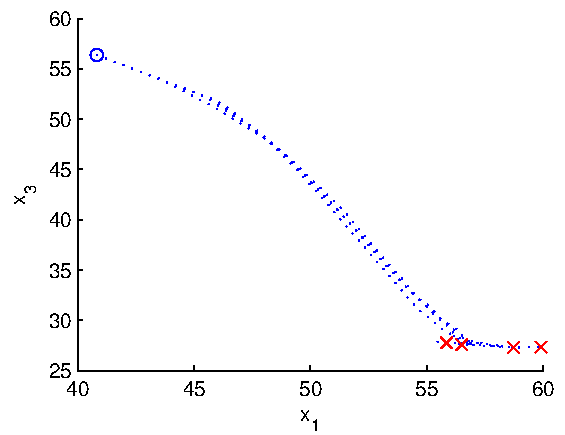
\includegraphics[width=0.45\columnwidth]{drone_example_rm.pdf}}
\subfloat[]{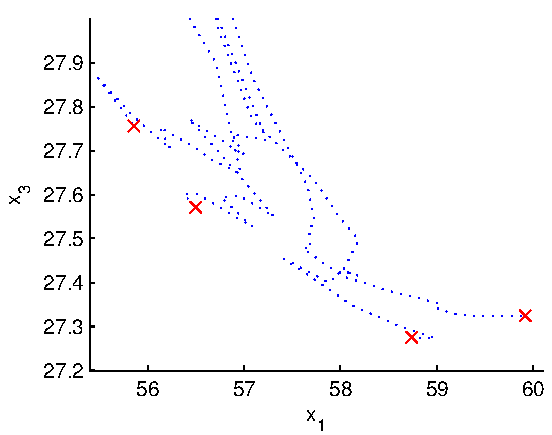
\includegraphics[width=0.45\columnwidth]{drone_example_rm_zoom.pdf}}
\caption{Four particle trajectories simulated from the same starting point using $\lgexpsf=0.3$, as used in the resample-move proposal stage. The second panel shows a close-up of the final states. This example uses the terrain tracking model from section~\ref{sec:numsim:tracking}, showing one horizontal and the vertical state component. Prior states are shown with circles and posterior states with crosses.}
\label{fig:drone_rm_example}
\end{figure}



\subsection{Step Size Selection}

An important practical consideration for implementing Gaussian flow sampling is how the sizes of the pseudo-time steps are chosen. State updates are calculated using local Gaussian approximations of the sequence density, with a best-case achieved with infinitesimally small steps between these approximations. In practice, the number of steps needs to be kept fairly low, to minimise the computational burden. In some instances, it may be sufficient to use a fixed step size, or a predetermined time grid chosen with a tuning run. However, an adaptive scheme is preferable for greatest efficiency.

Step size adaptation may be carried out separately for each particle. It is straightforward to see from \eqref{eq:approx_state_update}, \eqref{eq:deterministic_weight_update} and \eqref{eq:stochastic_weight_update} that two consecutive updates using the same values for $\lgmomapprox{\pt}$ and $\obapprox{\pt}$ are equivalent to a single update spanning both intervals. Thus, a large interval between update steps is equivalent to a number of shorter intervals with hypothetical intermediate update times aligned with those of the other particles.


\subsection{Local Error Estimates}

For adaptive step size control, a measure is required which estimates the local ``error'' introduced by using finite rather than infinitesimal step sizes. We consider the state update for the interval $[\pt_0,\pt_1]$, and distinguish between the ``ideal'' dynamics $\{\flowdriftapprox{\pt|\pt},\flowdiffuseapprox{\pt|\pt}\}$ which use a continuously updated approximation, and the actual dynamics $\{\flowdriftapprox{\pt|\pt_0},\flowdiffuseapprox{\pt|\pt_0}\}$ which use the approximation formed at $\pt_0$. Integrating the different between the two resulting SDEs, we find that the error introduced by using finite step sizes is,
%
\begin{IEEEeqnarray}{rCl}
 \lserror{\pt_1}{\pt_0} & = & \int_{\pt_0}^{\pt_1} \left[ \flowdriftapprox{l|\pt_0}(\ls{l}) - \flowdriftapprox{l|l}(\ls{l}) \right] dl + \int_{\pt_0}^{\pt_1} \left[ \flowdiffuseapprox{l|\pt_0} - \flowdiffuseapprox{l|l} \right] d\flowbm{l} \nonumber      .
\end{IEEEeqnarray}
%
The integrands are both equal to $0$ at $\pt_0$. Hence, approximating each over the interval by half its final value, we arrive at the following rough estimate for the error introduced by the update,
%
\begin{IEEEeqnarray}{rCl}
 \widehat{\lserror{\pt_1}{\pt_0}} & = & \half \left( \flowdriftapprox{\pt_1|\pt_0}(\ls{\pt_1}) - \flowdriftapprox{\pt_1|\pt_1}(\ls{\pt_1}) \right) (\pt_1-\pt_0) + \half \left( \flowdiffuseapprox{\pt_1|\pt_0} - \flowdiffuseapprox{\pt_1|\pt_1} \right) \int_{\pt_0}^{\pt_1} d\flowbm{l} \nonumber \\
 & \approx & \half (\pt_1-\pt_0) \left( \flowdriftapprox{\pt_1|\pt_0}(\ls{\pt_1}) - \flowdriftapprox{\pt_1|\pt_1}(\ls{\pt_1}) \right) + \half (\pt_1-\pt_0)^{\half} \left( \flowdiffuseapprox{\pt_1|\pt_0} - \flowdiffuseapprox{\pt_1|\pt_1} \right) \snchange{\pt_0,\pt_1} \nonumber       .
\end{IEEEeqnarray}
%
The last line follows from the definition of $\snchange{\pt_0,\pt_1}$ using approximations for small $(\pt_1-\pt_0)$,
%
\begin{IEEEeqnarray}{rCl}
 \snchange{\pt_0,\pt_1} & = & \frac{ \int_{\pt_0}^{\pt_1} \dsf^{\half}\exp\left\{ -\half \dsf (\pt_1-\pt_0) \right\} d\flowbm{\pt} }{ 1-\exp\left\{-\dsf(\pt_1-\pt_0)\right\} } \nonumber \\
 & \approx & \frac{ \dsf^{\half} \int_{\pt_0}^{\pt_1}d\flowbm{\pt} }{ \left[\dsf(\pt_1-\pt_0)\right]^{\half} } \nonumber \\
 \int_{\pt_0}^{\pt_1}d\flowbm{\pt} & \approx & (\pt_1-\pt_0)^{\half} \snchange{\pt_0,\pt_1} \nonumber      .
\end{IEEEeqnarray}

This formula also indicates that for small steps, the stochastic term is likely to dominate, and thus that the discretisation error can be reduced by setting $\dsf=0$.



\subsection{Step Size Control}

Pseudo-time step sizes may now be adjusted so that the magnitude of the local error estimate is kept below a threshold. For this purpose, step size control mechanisms may be borrowed directly from well-established numerical integration algorithms for solving differential equations.

One method found to be effective, inspired by \citep{Shampine1997}, is to increment pseudo-time by,
%
\begin{IEEEeqnarray}{rCl}
 \pt_1 & = & \pt_0 + \Delta\pt \label{eq:pseudo_time_update}     ,
\end{IEEEeqnarray}
%
and having calculated the new state, then update the step size $\Delta\pt$ according to,
%
\begin{IEEEeqnarray}{rCl}
 \Delta\pt & \leftarrow & \Delta\pt \times a \left(\frac{\magdet{ \widehat{\lserror{\pt_1}{\pt_0}} }}{ e_{\text{tol}} } \right)^b \nonumber      .
\end{IEEEeqnarray}
%
The parameters $a$, $b$ and $e_{\text{tol}}$ are constant: $e_{\text{tol}}$ is the tolerance for the local error whereas $a$ and $b$ determine the response in the step size to deviations of the error estimate away from $e_{\text{tol}}$. Enforcing a maximum and minimum step size is also judicious.



\section{Applications in Particle Filtering}

Our motivating purpose for studying particle flows is for use in filtering. We consider a standard discrete-time Markovian state space model in which the transition, observation and prior models have closed-form densities,
%
\begin{IEEEeqnarray}{rCl}
 \ls{\ti} & \sim & \transden(\ls{\ti} | \ls{\ti-1}) \label{eq:td} \\
 \ob{\ti} & \sim & \obsden(\ob{\ti} | \ls{\ti})   \label{eq:od} \\
 \ls{1} & \sim & \priorden(\ls{1})                  \label{eq:pd}      ,
\end{IEEEeqnarray}
%
where the random variable $\ls{\ti}$ is the hidden state of a system at time $\ti$, and $\ob{\ti}$ is an incomplete, noisy observation.

\subsection{Existing Approaches}

The approach taken by \cite{Daum2008,Daum2011d,Daum2013,Reich2011,Reich2012a} is to apply particle flow sampling directly to the filtering density. Assume that a set of unweighted particles exists approximating $\den(\ls{\ti-1}|\ob{1:\ti-1})$. The predictive density at the next step is related by,
%
\begin{IEEEeqnarray}{rCl}
 \den(\ls{\ti}|\ob{1:\ti-1}) & = & \int \den(\ls{\ti}|\ls{\ti-1}) \transden(\ls{\ti-1}|\ob{1:\ti-1}) d\ls{\ti-1}     ,
\end{IEEEeqnarray}
%
which can thus be sampled by simply drawing $\ls{\ti}\pss{i} \sim \transden(\ls{\ti}|\ls{\ti-1}\pss{i})$ for each particle and then marginalising (i.e. discarding) the old states. Defining this predictive density as the prior and the filtering density as the posterior, a particle flow is used to sample from,
%
\begin{IEEEeqnarray}{rCl}
 \den(\ls{\ti}|\ob{1:\ti}) & = & \frac{\den(\ls{\ti}|\ob{1:\ti-1}) \obsden(\ob{\ti}|\ls{\ti})}{\nconst{\ti}}      .
\end{IEEEeqnarray}
%
The difficulty with this approach is that finding an appropriate flow generally requires at least the prior and often also its gradient and Hessian to be calculable pointwise. This is not the case for the predictive density, $\den(\ls{\ti}|\ob{1:\ti-1})$. (Note that we could use a Monte Carlo approximation of this density, but the resulting algorithm has a complexity of $\bigo{\numpart^2}$ in the number of particles.) \cite{Reich2011,Reich2012a} address this by making analytical approximations of this density as a Gaussian or Gaussian mixture, in the spirit of an ensemble or mixture Kalman filter. \cite{Daum2008,Daum2011d,Daum2013} use a number of methods, including Gaussian approximations and various numerical approximations \citep{Daum2009c}. These approximations alter the distribution of the particles. The filter is no longer \emph{exact}, in the sense of returning a correctly weighted set of particles representing the posterior and providing asymptotically consistent estimates of posterior expectations.

In addition, the existing particle flow algorithms do not fall within the framework of ordinary particle filters. They only provide us with an estimate of the marginal filtering density $\den(\ls{\ti}|\ob{1:\ti})$, rather than the more conventional path filtering density $\den(\ls{1:\ti}|\ob{1:\ti})$. This may sometimes be all that is needed, but on other occasions samples of the entire path are essential, for example for smoothing or parameter estimation schemes \cite{Kitagawa1996,Andrieu2010}.

In this work, we use particle flow sampling within the standard particle filtering framework, thus restoring path sampling and voiding the need for additional layers of approximations. This is achieved by applying the particle flow sampling to the optimal importance density instead of the filtering density directly.

\subsection{A Generic Particle Filter}

A conventional particle filter \citep{Cappe2007,Doucet2009} uses importance sampling to estimate distributions recursively over the path of the state variables, $\ls{1:\ti}=\{\ls{1}, \dots, \ls{\ti}\}$, such that,
%
\begin{IEEEeqnarray}{rCl}
 \sum_{i=1}^{\numpart} \npw{\ti}\pss{i} \phi(\ls{1:\ti}\pss{i}) & \rightasconverge & \int \postden(\ls{1:\ti}) \phi(\ls{1:\ti}) d\ls{1:\ti}      \nonumber       .
\end{IEEEeqnarray}
%
Each step begins by selecting a set of ancestors $\{\anc{\ti}{i}\}$ from amongst the ($\ti-1$)th step particles according to the corresponding weights. Next, a new state is proposed for each particle from an importance density,
%
\begin{IEEEeqnarray}{rCl}
 \ls{\ti}\pss{i} \sim \impden(\ls{\ti} | \ls{\ti-1}\pss{\anc{\ti}{i}}, \ob{\ti})
\end{IEEEeqnarray}
%
and this is concatenated to the ancestral path to form the new particle,
%
\begin{IEEEeqnarray}{rCl}
 \ls{1:\ti}\pss{i} \leftarrow \left\{ \ls{1:\ti-1}\pss{\anc{\ti}{i}},  \ls{\ti}\pss{i} \right\}     .
\end{IEEEeqnarray}
%
An importance weight is then assigned to the particle to account for the discrepancy between importance and target distributions,
%
\begin{IEEEeqnarray}{rCl}
 \pw{\ti}\pss{i} & = & \frac{ \den(\ls{1:\ti}\pss{i} | \ob{1:\ti}) }{ \den(\ls{1:\ti}\pss{\anc{\ti}{i}} | \ob{1:\ti}) \impden(\ls{\ti}\pss{i} | \ls{\ti}\pss{\anc{\ti}{i}}, \ob{\ti}) } \nonumber \\
 & \propto & \frac{ \transden(\ls{\ti}\pss{i} | \ls{\ti-1}\pss{\anc{\ti}{i}}) \obsden(\ob{\ti}|\ls{\ti}\pss{i}) }{ \impden(\ls{\ti}\pss{i} | \ls{\ti-1}\pss{\anc{\ti}{i}}, \ob{\ti}) }     .
\end{IEEEeqnarray}

As in the case of any importance sampling, the simplest choice for the importance density is to use the prior, in this case the transition density,
%
\begin{IEEEeqnarray}{rCl}
 \impden(\ls{\ti} | \ls{\ti-1}\pss{\anc{\ti}{j}}, \ob{\ti}) = \transden(\ls{\ti} | \ls{\ti-1}\pss{\anc{\ti}{j}})     .
\end{IEEEeqnarray}
%
This is the bootstrap filter of \cite{Gordon1993}. It is often inefficient, especially when the variance of the transition density is much greater than that of the observation density. In this situation, the samples are widely spread over the state space, and only a few fall in the region of high likelihood. This results in a high variance of the weights and posterior estimates, and poor filter performance.

It was shown in \citep{Doucet2000a}, and references therein, that the weight variance is minimised by using the conditional posterior as the importance distribution,
%
\begin{IEEEeqnarray}{rCl}
 \impden(\ls{\ti} | \ls{\ti-1}\pss{\anc{\ti}{j}}, \ob{\ti}) & = & \den(\ls{\ti} | \ls{\ti-1}\pss{\anc{\ti}{j}}, \ob{\ti})      ,
\end{IEEEeqnarray}
%
resulting in the following weight formula,
%
\begin{IEEEeqnarray}{rCl}
 \pw{\ti}\pss{j} & \propto & \den(\ob{\ti} | \ls{\ti-1}\pss{\anc{\ti}{j}}) \nonumber \\
           & \propto & \int \obsden(\ob{\ti} | \ls{\ti}) \transden(\ls{\ti} | \ls{\ti-1}\pss{\anc{\ti}{j}}) d\ls{\ti}      .
\end{IEEEeqnarray}
%
This choice is therefore known as the optimal importance density (OID). It may be sampled and the weights calculated analytically when the observation density is linearly dependent on the state and both transition and observation densities are Gaussian. (The state need not be linearly dependent on the previous state.) However, for most models this density can neither be calculated, nor efficiently sampled. Thus, it is common to use methods such as linearisation and the unscented transform to approximate the OID with a Gaussian density, in an equivalent manner to extended and unscented Kalman filters \citep{Doucet2000a,Merwe2000}. These approximations may work well when the OID is unimodal, and the observation nonlinearity is weak, but can otherwise perform worse even than the bootstrap filter.

Particle filter performance is often characterised by the effective sample size (ESS) at each time step. This is defined as,
%
\begin{IEEEeqnarray}{rCl}
 \ess{\ti} & = & \frac{ 1 }{ \sum_i \npw{\ti}\pss{i}{}^2 }     ,
\end{IEEEeqnarray}
%
Intuitively, this is an estimate of the number of particles which would be present in an equivalent set comprised of independent, unweighted samples. It takes a value between $1$ (which is bad) and the number of filtering particles, $\numpart$ (which is good).



\subsection{Gaussian Flow Approximations to the Optimal Importance Density}

Note, in this section we omit for clarity subscript $\ti$ on variables which vary with $\pt$. Applying the Gaussian flow sampling to the OID is straightforward, setting the prior to be the transition density and the likelihood the observation density,
%
\begin{IEEEeqnarray}{rCl}
 \den(\ls{\ti}|\ls{\ti-1}\pss{i},\ob{\ti}) & = & \frac{ \transden(\ls{\ti}|\ls{\ti-1}\pss{i}) \obsden(\ob{\ti}|\ls{\ti}) }{ \nconst{}(\ls{\ti-1}\pss{i}) }     .
\end{IEEEeqnarray}
%
The only modification required to the standard process is in the weight formulas. Although the particle flow is calculated based on the OID sequence, the target density for the importance sampler is now replaced by the filtering density. With this simple change, the required weight formulas become,
%
\begin{IEEEeqnarray}{rCl}
 \pw{\pt_1} & \propto & \pw{\pt_0} \times \frac{ \obsden(\ob{\ti} | \ls{\pt_1})^{\pt_1} \transden(\ls{\pt_1} | \ls{\ti-1}) }{ \obsden(\ob{\ti} | \ls{\pt_0})^{\pt_0} \transden(\ls{\pt_0} | \ls{\ti-1}) } \times \frac{ \normal{\ls{\pt_0}}{\lsmnapprox{\pt_0}}{\lsvrapprox{\pt_0}} }{ \normal{\ls{\pt_1}}{\lsmnapprox{\pt_1}}{\lsvrapprox{\pt_1}} } \label{eq:PPPF_stochastic_weight_update}       ,
\end{IEEEeqnarray}
%
for the stochastic case, and,
%
\begin{IEEEeqnarray}{rCl}
 \pw{\pt_1} & \propto & \pw{\pt_0} \times \frac{ \obsden(\ob{\ti} | \ls{\pt_1})^{\pt_1} \transden(\ls{\pt_1} | \ls{\ti-1}) }{ \obsden(\ob{\ti} | \ls{\pt_0})^{\pt_0} \transden(\ls{\pt_0} | \ls{\ti-1}) } \times \sqrt{\frac{\determ{\lsvrapprox{\pt_1}}}{\determ{\lsvrapprox{\pt_0}}}} \label{eq:PPPF_deterministic_weight_update}       ,
\end{IEEEeqnarray}
%
for the deterministic case.

\section{Comparisons with Other Work}

The Gaussian flow importance sampling method shares a number of features with existing algorithms. Here we summarise and highlight some of the similarities and differences.

The concept of introducing intermediate distributions between the predictive and filtering densities has been employed in numerous ways, under the names ``annealing'' \citep{Neal2001,Deutscher2000,Gall2007}, ``tempering'' \citep{DelMoral2006}, ``bridging distributions'' \citep{Godsill2001b} and ``progressive corrections'' \citep{Oudjane2000}. These all use a discrete set of intermediate times, and do not consider the continuous evolution of the states. Furthermore they rely on importance sampling, Metropolis-Hastings and kernel sampling, all stochastic mechanisms, to advance between these pseudo-times. None of them include a deterministic component for updating the state. Moreover, these methods all rely on moving the particles through pseudo-time on the same fixed grid, and make use of intermediate resampling and interaction steps. In this work, each particle is moved entirely independently and with adaptive step sizes.

There is no reason why a particle flow could not be used in combination with an annealing scheme. The particles would be moved independently through pseudo-time, but periodically they are stopped and an intermediate resampling or resample-move step is performed. Particle flow and annealing should be seen as complementary rather than competing algorithms.

The particle flow and optimal transport methods of \citep{Daum2008,Daum2011d,Reich2011,Reich2012a} use similar particle flow ideas to address the task of filtering as we do here. The essential differences in this work are:
%
\begin{itemize}
  \item We target the optimal importance density rather than the filtering density directly. The OID is known pointwise up to a normalising constant, and thus we avoid the need for one layer of approximation.
  \item In \citep{Daum2008,Daum2011d,Reich2011,Reich2012a}, particle flow samples are used directly to form an approximation of the posterior, with a consequent result that asymptotic properties are lost. We use the particle flow samples as the input to an importance sampler, and correct for the difference between the implied importance density and the posterior density with an appropriate importance weight. This was suggested by \cite{Reich2012}.
  \item Rather than relying on numerical integration, we use the Gaussian flow exclusively, as this has an analytical solution.
\end{itemize}



\section{Simulations}

Numerical testing using simulated data is presented to demonstrate the efficacy of Gaussian flow sampling for particle filtering. The aim in developing this method is to provide a more efficient particle filter for challenging nonlinear models. In such cases, simple Gaussian approximations often work poorly, because the posterior filtering distributions of such models can assume complex and irregular shapes.

Our primary indicator of performance will be the average effective sample size, measured before resampling. RMSE values using the empirical particle mean as a point estimate are also included. However, they should be treated with caution, since when a distribution is irregular the particle mean may be distant from the true value even if the particles are drawn from it perfectly (see figure~\ref{fig:rmse_fail} for an illustration of this effect). All comparisons are conducted by adjusting the number of filter particles such that the running times for the various algorithms are roughly equal.
%
\begin{figure}
\centering
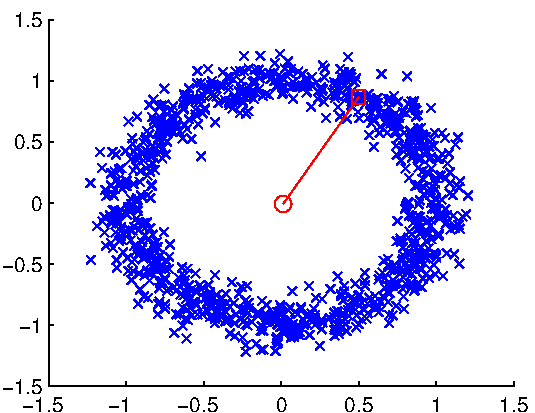
\includegraphics[width=0.7\columnwidth]{rmse_fail.pdf}
\caption{An illustration of how RMSE can be a misleading performance measure. A large number of samples (crosses) are drawn from the same distribution as the true value (square). The resulting sample mean (circle) is a very poor estimate of the true value, and the RMSE is large.}
\label{fig:rmse_fail}
\end{figure}

The following particle filters (and their respective importance densities) are used in testing:
\begin{itemize}
        \item A bootstrap filter (BF), using the transition density.
        \item An extended particle filter (EPF), using a Gaussian density chosen by linearisation about the predictive mean, in the style of an extended Kalman filter.
        \item An unscented particle filter (UPF), using a Gaussian density chosen using the unscented transform, in the style of an unscented Kalman filter.
        \item A Laplace approximation particle filter (LAPF), using a Gaussian density chosen by truncation of the Taylor series of the log of the unnormalised OID around a local maximum \citep{Doucet2000a}. Gradient ascent is used to locate the maximum.
        \item A Gaussian flow particle filter (GFPF), using the the Gaussian flow importance sampling method.
\end{itemize}



\subsection{A Illustrative Problem}

\subsubsection{The Model}

First we study a modified form of the model used by \citet{Mihaylova2011}, which is a multivariate extension of the nonlinear benchmark model of \citep{Kitagawa1991}. The transition and observation functions are,
%
\begin{IEEEeqnarray}{rCl}
 \transfun(\ls{\ti-1}) & = & \half \ls{\ti-1} + 25 \frac{ \sum_d \ls{\ti-1,d} }{ 1 + \left(\sum_d \ls{\ti-1,d}\right)^2 } + 8 \cos(1.2 \ti) \nonumber \\
 \obsfun(\ls{\ti})_d   & = & \alpha \left( \ls{\ti,2d-1}^2 + \ls{\ti,2d}^2 \right) \nonumber      ,
\end{IEEEeqnarray}
%
where $\ls{\ti,d}$ and $\obsfun(\ls{\ti})_d$ are the $d$th components of the state vector and observation function respectively. A $10$-dimensional state and a $5$-dimensional observation were used. The transition and observation densities are Gaussian with $\lgmtv = 100 \times I$ and $\lgmov = I$.

This model is particularly challenging because the observations give us information only about the magnitudes of a set of sub-vectors of the state. Information about the corresponding bearing is only available via the transition model. Consequently, the region of high posterior probability corresponds to a ``thin'' section of the space bounding a hyper-sphere. A Gaussian density is a very poor approximation of this region. (See figure~\ref{fig:nlng_example_frame}.)

\subsubsection{Algorithms and Results}

Particle filters using extended or unscented Kalman-type importance densities fail immediately on this model; all the particles suffer numerical underflow of their weight due to states being sampled only in highly improbable regions. Tests were conducted on a BF, LAPF, and a GFPF. The GFPF used $\dsf=0$ and employed the adaptive step size method, typically requiring in the region of $10$ to $20$ state updates at each time step. Figure~\ref{fig:nlng_example_frame} shows the motion of the particles from the GFPF on a typical frame, and the awkward shape of the posterior mode. Table~\ref{tab:nlng_results} shows the average ESSs and RMSEs for each algorithm over 100 simulated data sets, each of 100 time steps.
%
\begin{table}
\centering
\begin{tabular}{l||c|c|c}
Algorithm                                & $N_F$ & ESS  & RMSE \\
\hline
Bootstrap                                & 18500 &  1.7 & 43.6 \\
Laplace Approximation                    &    70 &  1.7 & 42.8 \\
Gaussian Flow                            &   540 & 81.1 & 32.6 \\
\end{tabular}
\caption{Algorithm performance results on the multivariate benchmark model, showing number of filter particle ($N_F$), effective sample size (ESS), and root mean square error (RMSE).}
\label{tab:nlng_results}
\end{table}
%
\begin{figure}
\centering
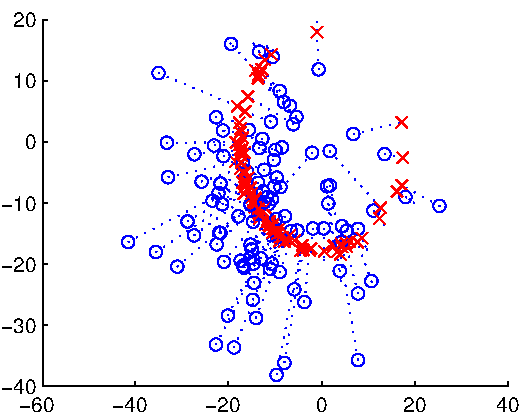
\includegraphics[width=0.7\columnwidth]{nlng_example_frame_deter.pdf}
\caption{An example of the GFPF particle motion running on the multivariate benchmark model, showing $2$ of the $10$ state dimensions. Prior states are shown with circles and posterior states with crosses.}
\label{fig:nlng_example_frame}
\end{figure}



\subsection{A Difficult Tracking Problem} \label{sec:numsim:tracking}

\subsubsection{The Model}

Next we consider tracking a small aircraft over a mapped landscape, an example inspired by \cite{Schon2005}. Time of flight and Doppler measurements from a radio transmitter on the aircraft provide accurate measurements of range $\rng{\ti}$, and range rate $\rngrt{\ti}$, but only a low resolution measurement of bearing $\bng{\ti}$. In addition, accurate measurements are made of the height above the ground $\hei{\ti}$. The profile of the terrain (i.e. the height of the ground above a datum at each point) has been mapped.

At $\ti$, the latent state for our model is,
%
\begin{IEEEeqnarray}{rCl}
 \ls{\ti} & = & \begin{bmatrix} \pos{\ti} \\ \vel{\ti} \end{bmatrix} \nonumber      ,
\end{IEEEeqnarray}
%
where $\pos{\ti}$ and $\vel{\ti}$ are the $3$-dimensional position and velocity of the aircraft respectively, and the observation is,
%
\begin{IEEEeqnarray}{rCl}
 \ob{\ti} & = & \begin{bmatrix} \bng{\ti} \\ \rng{\ti} \\ \hei{\ti} \\ \rngrt{\ti} \end{bmatrix}       .
\end{IEEEeqnarray}
%
The observation function is described by the following equations,
%
\begin{IEEEeqnarray}{rCl}
 \bng{\ti}   & = & \arctan\left(\frac{\pos{\ti,1}}{\pos{\ti,2}}\right) \nonumber \\
 \rng{\ti}   & = & \sqrt{ \pos{\ti,1}^2 + \pos{\ti,3}^2 + \pos{\ti,3}^2 } \nonumber \\
 \hei{\ti}   & = & \pos{\ti,3} - \terrain( \pos{\ti,1}, \pos{\ti,2} ) \nonumber \\
 \rngrt{\ti} & = & \frac{ \pos{\ti}\cdot\vel{\ti} }{ \rng{\ti} } \nonumber      ,
\end{IEEEeqnarray}
%
where $\terrain( \pos{\ti,1}, \pos{\ti,2} )$ is the terrain height at the corresponding horizontal coordinates. The four measurements are independent and the respective variances are $\left(\frac{\pi}{9}\right)^2$, $0.1^2$, $0.1^2$, $0.1^2$.

A linear Gaussian near-constant velocity transition model is used,
%
\begin{IEEEeqnarray}{rCl}
 \transden(\ls{\ti} | \ls{\ti-1}) & = & \normal{\ls{\ti}}{\lgmtm\ls{\ti-1}}{\lgmtv} \nonumber \\
\end{IEEEeqnarray}
%
\begin{IEEEeqnarray}{rCl}
 \lgmtm & = & \begin{bmatrix} I & I \\ 0 & I \end{bmatrix} \nonumber \\
 \lgmtv & = & 10 \begin{bmatrix} \frac{1}{3} I & \frac{1}{2} I \\ \frac{1}{2} I &\ I \end{bmatrix} \nonumber      .
\end{IEEEeqnarray}
%
For the simulations presented here, the terrain profile was modelled as a mixture of randomly-generated Gaussian blobs. An example is shown in figure~\ref{fig:drone_terrain_map}.

The accurate measurements of range, range rate and height constrain the region of high posterior probability to lie on a $3$ dimensional subspace, which can take some very irregular shapes (see figure~\ref{fig:drone_example_frame_deterministic}).
%
\begin{figure}
\centering
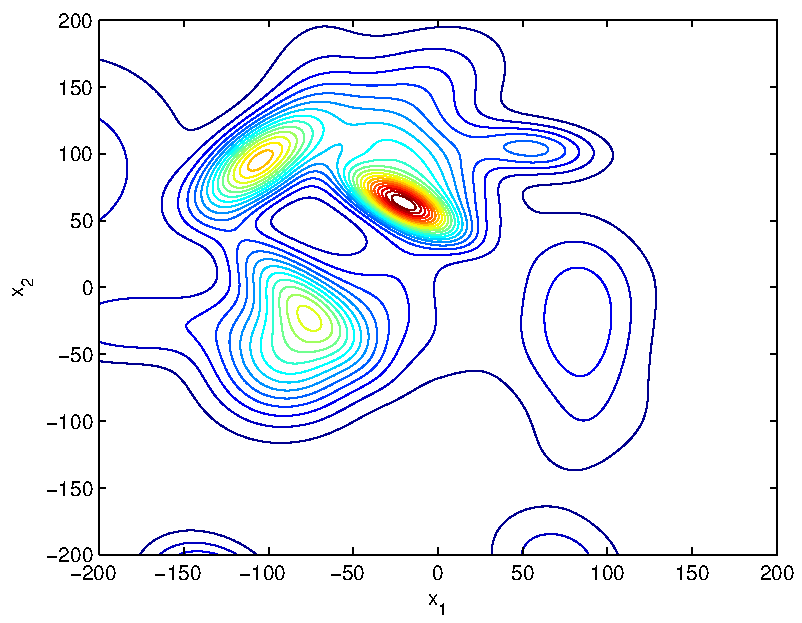
\includegraphics[width=0.7\columnwidth]{drone_terrain_map.pdf}
\caption{Contour plot of an example simulated terrain map.}
\label{fig:drone_terrain_map}
\end{figure}

\subsubsection{Algorithms and Results}

Particle filters using extended or unscented Kalman-type importance densities again did not perform well, with the EPF losing track immediately. Furthermore, the LAPF also performed particularly poorly as maximisation procedures struggle with the narrow mode. Tests were conducted on a BF, UPF, LAPF, and GFPF. The GFPF used $\dsf=0$ and employed the adaptive step size method, using in the region of $5$ to $10$ state updates at each time step.

Figure~\ref{fig:drone_example_frame_deterministic} shows the motion of the particles from the GFPF on a typical frame, and the awkward shape of the posterior mode.
%
\begin{figure}
\centering
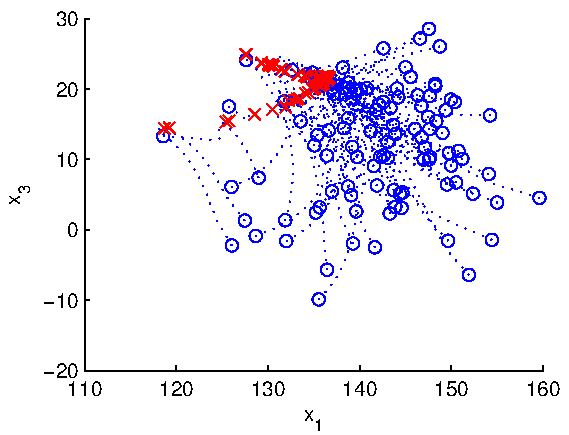
\includegraphics[width=0.7\columnwidth]{drone_example_frame_deter.pdf}
\caption{An example of the GFPF particle motion running on the terrain tracking model, showing one horizontal and the vertical state component. Prior states are shown with circles and posterior states with crosses.}
\label{fig:drone_example_frame_deterministic}
\end{figure}

Particle flow resample-move was also tested on this problem. Figure~\ref{fig:drone_example_frame_stochastic} shows the resulting stochastic motion of the particles. Using $\dsf=0.3$, roughly $25$--$50\%$ of the MH steps were accepted, giving us a richer particle set with which to approximate the filtering density. The RMSE performance was not significantly improved.
%
\begin{figure}
\centering
\subfloat[]{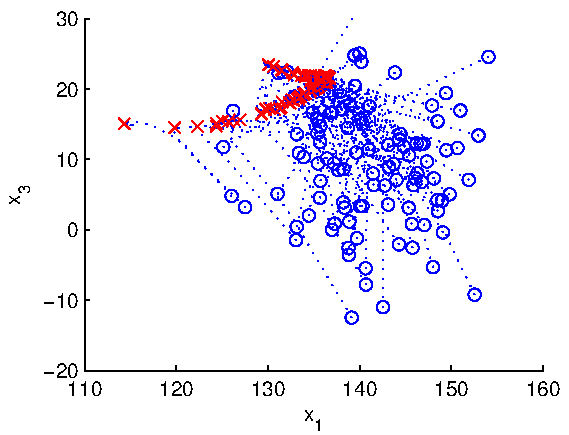
\includegraphics[width=0.45\columnwidth]{drone_example_frame.pdf}}
\subfloat[]{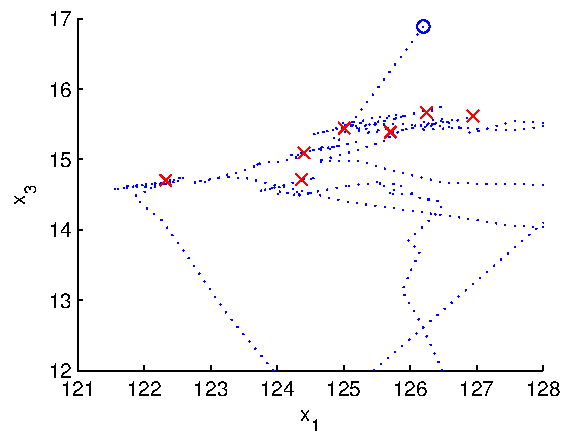
\includegraphics[width=0.45\columnwidth]{drone_example_frame_zoom.pdf}}
\caption{An example of the stochastic GFPF ($\dsf=0.3$) particle motion running on the terrain tracking model, showing one horizontal and the vertical state component. Prior states are shown with circles and posterior states with crosses. The second panel is a close-up showing the stochastic motion of the particles.}
\label{fig:drone_example_frame_stochastic}
\end{figure}

Table~\ref{tab:drone_results_gaussian} shows the average ESSs and RMSEs for each algorithm over 100 simulated data sets, each of 100 time steps using the Gaussian transition density.
%
\begin{table}
\centering
\begin{tabular}{l||c|c|c}
Algorithm                                & $N_F$ & ESS  & RMSE \\
\hline
Bootstrap                                &  6000 &  1.0 & 78.6 \\
Unscented Kalman                         &   460 &  2.4 & 70.2 \\
Laplace Approximation                    &    10 &  3.1 & 62.9 \\
Gaussian Flow                            &   180 & 56.4 & 22.3 \\
\end{tabular}
\caption{Algorithm performance results on the multivariate benchmark model, showing number of filter particle ($N_F$), effective sample size (ESS), and root mean square error (RMSE).}
\label{tab:drone_results_gaussian}
\end{table}



\subsection{A Heartbeat Inference Problem}

\subsubsection{The Model}

As a final example, we consider the problem of detecting heartbeats in a vibration signal for ballistocardiography. Measurements from an accelerometer are first partitioned into segments believed to contain a heartbeat, and a particle filter is then used to infer its properties. The ($\ti$)th heartbeat is modelled parametrically as the product of a squared-exponential envelope with amplitude $\amp{\ti}$ and width $\wid{\ti}$, and a sine wave carrier with frequency $\freq{\ti}$ and relative phase $\pha{\ti}$. The time shift of the centre of the heartbeat within the measurement window is $\del{\ti}$, and the sensor exhibits a D.C. bias $\bias{\ti}$ which varies slowly over time. The resulting observation function is highly nonlinear, with the ($d$)th component given by,
%
\begin{IEEEeqnarray}{rCl}
 \obsfun(\ls{\ti})_d & = & \amp{\ti} \exp\left\{ -\frac{ (T\,d - \del{\ti})^2 }{ 2\wid{\ti}^2 } \right\} \sin\left( \freq{\ti}(T\,d - \del{\ti}) + \pha{\ti} \right) + \bias{\ti} \nonumber      ,
\end{IEEEeqnarray}
%
where $T$ is the sampling period of the sensor. Each observation consists of $50$ time samples and the observation density is modelled as a Gaussian with a covariance matrix $0.2^2 I$. An example heartbeat simulated from this model is shown in figure~\ref{fig:sineha_example_beat}.
%
\begin{figure}
\centering
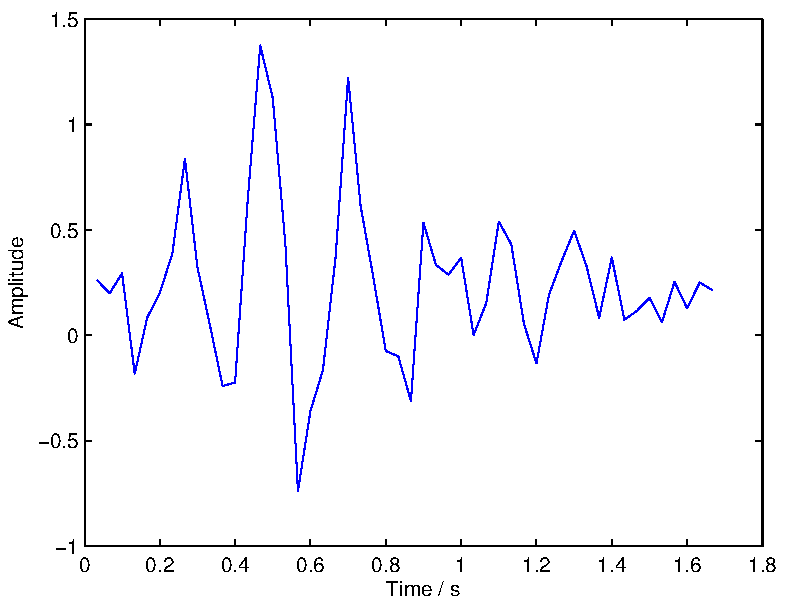
\includegraphics[width=0.7\columnwidth]{sineha_example_beat.pdf}
\caption{An example heartbeat simulated from the model.}
\label{fig:sineha_example_beat}
\end{figure}

The latent state is,
%
\begin{IEEEeqnarray}{rCl}
 \ls{\ti} & = & \begin{bmatrix} \amp{\ti} & \wid{\ti} & \del{\ti} & \freq{\ti} & \pha{\ti} & \bias{\ti} \end{bmatrix}^T      .
\end{IEEEeqnarray}
%
The transition density is factorised into independent terms, with $\freq{\ti}$, $\pha{\ti}$ and $\bias{\ti}$ evolving according to a Gaussian random walk, and $\wid{\ti}$ according to a geometric random walk (i.e. with a log-normal density), while $\del{\ti}$ and $\amp{\ti}$ are gamma distributed with no dependence on their past values. The resulting likelihood and filtering densities are highly multi-modal.

\subsubsection{Algorithms and Results}

Particle filters using extended or unscented Kalman-type importance densities fail immediately on this model due to the highly multi-modal filtering distribution. Tests were conducted on a BF, LAPF, and GFPF. For the GFPF, $\dsf=0$ and the transition density is approximated by a Gaussian using the method described in section~\ref{sec:non_gaussian_models}. The GFPF uses the adaptive step size method and made in the region of $5$ to $15$ state updates per time step, with the exception of a few particles which tended to ``get stuck'' in low probability regions and which were discarded after 50 steps.

Figure~\ref{fig:sineha_example_frame} shows the motion of the particles from the GFPF on a typical frame. Table~\ref{tab:sineha_results} shows the average ESSs and RMSEs for each algorithm over 100 simulated data sets, each of 100 time steps.
%
\begin{table}
\centering
\begin{tabular}{l||c|c|c}
Algorithm                                & $N_F$ & ESS  & RMSE \\
\hline
Bootstrap                                & 15000 &  7.6 &  2.0 \\
Laplace Approximation                    &   200 &  8.8 &  2.0 \\
Gaussian Flow                            &   800 & 72.8 &  1.4 \\
\end{tabular}
\caption{Algorithm performance results on the multivariate benchmark model, showing number of filter particle ($N_F$), effective sample size (ESS), and root mean square error (RMSE).}
\label{tab:sineha_results}
\end{table}
%
\begin{figure}
\centering
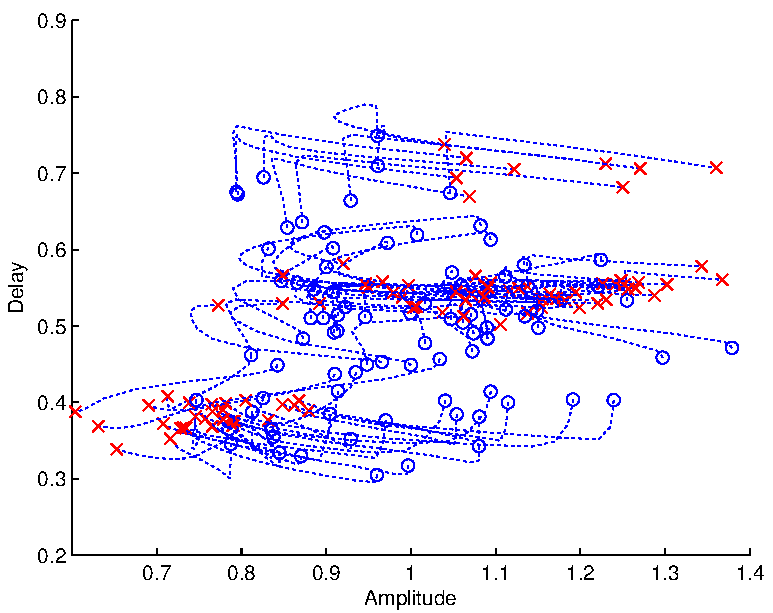
\includegraphics[width=0.7\columnwidth]{sineha_example_frame.pdf}
\caption{An example of the GFPF particle motion running on the heartbeat inference model, showing amplitude and delay state components. Prior states are shown with circles and posterior states with crosses.}
\label{fig:sineha_example_frame}
\end{figure}



\section{Extensions and Future Work}

Particle flow sampling is only suitable for continuous variables. It should be noted that when the latent state is mixed, with both discrete and continuous components, it is straightforward to sample the discrete component first and then use a particle flow for the continuous part. Furthermore, the Gaussian flows used in this work perform best when the prior and likelihood are Gaussian. A number of heavy tailed distributions, including student-t and alpha-stable, can be written as a scale mixture of normals, such that they are Gaussian conditional on an auxiliary scale variable. If this scale variable is sampled first, then a Gaussian flow may be then be used to sample the state.

In this work we have used the Gaussian flow exclusively, due to its desirable analytical solution. This has proven very effective on a number of examples, in particular when the prior and likelihood have a Gaussian form but the observation function is highly nonlinear. However, on non-Gaussian models it is harder to apply and generally yields less improvement over standard methods. Future research will focus on the use of other choices of particle flow, and in finding methods to weight the particles correctly when numerical integration is required.




\section{Summary and Conclusions}

We have detailed the use of Gaussian particle flows for sampling approximately from a distribution, and applied them to draw from the optimal importance density of a particle filter. The simulations presented in the previous section demonstrate that this procedure is capable of achieving better particle approximations (i.e. higher effective sample sizes) than simpler particle filters (which use a simple Gaussian importance density) on a class of challenging state space models.

The algorithm exploits the fact that the Gaussian flow may be integrated analytically to avoid numerical integration, and uses an importance sampling framework to correct for the necessary approximations. By applying particle flow sampling to the OID in a particle filter, we avoid the need to make additional approximations of the filtering density.

The models for which the method is most effective are those with Gaussian prior and likelihood but highly nonlinear dependence between the observations and latent state. For this class, the performance improvement relative to the simpler algorithms with an equal processing time is very great. Moreover, the requisite Gaussian approximation is ``obvious'', simply a linearisation of the observation function, meaning that the algorithm requires almost no tuning (the tolerance for the adaptive step-size selection process is the only critical parameter). With non-Gaussian model densities, the performance gains from the Gaussian flow method are more modest, and when more drastic approximations are required a greater degree of algorithm tuning is required, such as limiting the variance of the approximation to prevent instability.



\bibliographystyle{chicago}
\bibliography{D:/pb404/Dropbox/PhD/thesisbib}
%\bibliography{/home/pete/Dropbox/PhD/OTbib}

\end{document}
